% !TeX encoding = UTF-8
% 此文件从2022.8开始

\chapter{李群与李代数初步}\label{chlg}

李群是由挪威数学家Sophus Lie最早研究的;
它是一类重要的微分流形,其线性化后便是李代数.
李群内容十分丰富,我们不可能详细叙述整个理论,
只能介绍一些基本概念、重要定理.
详尽论述可本章末参考文献;
所有忽略的定理证明可在上述文献中查到.
由于抽象指标记号对于有较多缩并、求导的运算较为合适,
而李群中较少用到这类运算;所以本章不用抽象指标,而采用\S \ref{chmla:sec_tensor}记号.

\index[physwords]{李群}
\index[physwords]{李代数}

\section{李群与李代数定义}\label{chlg:sec_definition}

\begin{definition}\label{chlg:def_lg}
    设$G$是一个非空集合,如果
    {\bfseries (1)} $G$是一个群;{\bfseries (2)} $G$是$m$维$C^\infty$实流形;
    {\bfseries (3)} 群乘法和求逆是$C^\infty$可微的,
    即:映射$gh$和$g^{-1}$是$G$上的$C^\infty$映射,其中$\forall g,h\in G$.
    则称$G$是一个$m$维实{\heiti 李群}.
    李群{\heiti 维数}是指它作为流形的维数.

    若李群的拓扑结构是紧致的(见定义\ref{chtop:def_compact}),则称$G$为{\heiti 紧致李群}.
    
    若上述条件只在$G$的包含幺元局部连通开集$U$成立,则称$U$是{\heiti 局部李群}.
       
    若将上述定义中$C^\infty$改为$C^0$,则称$G$为{\heiti 拓扑群}.
    
    若将上述定义中$C^\infty$改为\uwave{复解析},把底流形改为\uwave{复流形},
    则称$G$为{\heiti 复李群}.
\end{definition}

我们知道任一$m$维复流形(见\S\ref{chcx:sec_cxmanifold}),
都有自然方式看成$2m$维实流形;
$g\cdot h^{-1}$是复解析映射,自然也是实解析映射,那自然是$C^\infty$的,
因此$G$是$2m$维实李群.反之未必.


\begin{definition}\label{chlg:def_la}
    设$\mathscr{G}$是数域$\mathbb{F}$ 
    上的$m$维线性空间,$\forall X,Y \in \mathscr{G}$,有$\mathscr{G}$中
    唯一一个元素$[X,Y]$与之对应({\heiti 封闭性}),$[X,Y]$称为
    换位子或{\heiti 李积},且满足如下性质:
    
    {\bfseries (1)} 反对称性:$[X,Y]=-[Y,X]$;
    
    {\bfseries (2)} 双$\mathbb{F}$-线性:$[ X + k Y, Z]= [X, Z]+ k[Y, Z]$,常常省略前缀“$\mathbb{F}$-”;
    
    {\bfseries (3)} Jacobi恒等式:$\bigl[X,[Y,Z]\bigr]+\bigl[Y,[Z,X]\bigr]+\bigl[Z,[X,Y]\bigr]=0$.
    
\noindent    其中$\forall X, Y, Z \in \mathscr{G}$,$\forall k \in \mathbb{F}$,
    则称$\mathscr{G}$是一个$m$维{\heiti 李代数}.
    李代数维数是指它作为线性空间的维数.
    若$\mathbb{F}$是实数域,则称$G$为{\heiti 实李代数};
    若$\mathbb{F}$是复数域,则称$G$为{\heiti 复李代数};
    我们不考虑其它数域情形.
    
    紧致李群的李群李代数(定义见第\pageref{chlg:eqn_LgXY}页,
    及定理\ref{chlg:thm_Lie3inv})称为{\heiti 紧致李代数}.
\end{definition}


由(1)和(2)可知,李积对第二个因子也是线性的,即李积是双线性的.
\begin{equation*}
    [Z,  X + k Y]= -[ X + k Y, Z]= -[X, Z]- k[Y, Z] = [Z,X]+ k[Z, Y].
\end{equation*}

%李群与李代数最基本的关系可见\S \ref{chlg:sec_Lie3thm}的几个定理.


\begin{definition}
    设有两个李群$G$和$H$,且$H\subset G$.如果 {\bfseries (1)} $H$是$G$的子群;
    {\bfseries (2)} 恒等映射${\rm id}:H\to G$是嵌入子流形.则称$H$为$G$的{\heiti 李子群}.
    
    如果映射${\rm id}:H\to G$是正则嵌入子流形,则称$H$为$G$的{\heiti 拓扑李子群}.
\end{definition}

\begin{definition}
    设李群$H$是李群$G$的李子群,如果$H$还是$G$的闭子集(见定义\ref{chtop:def_closedset}),
    则称$H$为$G$的{\heiti 闭子群}.
\end{definition}

\begin{definition}
    设有李代数$\mathscr{G}$,$\mathscr{H}$是它的子集;
    如果$\forall \mathfrak{h}_1,\mathfrak{h}_2\in \mathscr{H}$有
    $[\mathfrak{h}_1,\mathfrak{h}_2]\in \mathscr{H}$,
    那么称$\mathscr{H}$是$\mathscr{G}$的{\heiti 李子代数}.
\end{definition}

\begin{definition}
    设有李代数$\mathscr{G}$及其子代数$\mathscr{H}$,如果
    $   [\mathfrak{g},\mathfrak{h}]\in  \mathscr{H},\ 
    \forall \mathfrak{g}\in \mathscr{G}, \ \forall\mathfrak{h}\in\mathscr{H}$;
    则称$\mathscr{H}$是$\mathscr{G}$的{\heiti 理想}(ideal).
\end{definition}
因李代数具有反对称性($[X,Y]=-[Y,X]$),故理想不分左、右,全部是双边理想.
李代数中理想的概念与群理论中正规子群(见定义\ref{chtop:def_normal-subgroup})概念相当.



\index[physwords]{李代数!单纯}
\index[physwords]{李代数!半单纯}
\index[physwords]{李代数!理想}

\begin{definition}
    设有李群$G$及其李代数$\mathscr{G}$.
    若$G$不含有正规李子群(除群$G$本身和单位元$e$构成的子群之外),
    则称$G$是{\heiti 单李群}(英文是simple,也译为“单纯”).
    若$G$不含有{\kaishu 可对易}正规李子群(除单位元$e$构成的子群之外),
    则称$G$是{\heiti 半单李群}(semi-simple).
\end{definition}

\begin{definition}    
    如果$\mathscr{G}$不含有理想(除$\mathscr{G}$本身和零元$\{0\}$构成的理想之外),
    则称$\mathscr{G}$是{\heiti 单李代数}.
    如果$\mathscr{G}$不含\uwave{非零}\uwave{可对易}理想,
    则称$\mathscr{G}$是{\heiti 半单李代数}.
\end{definition}


设有李代数$\mathscr{G}$,$\mathscr{H}$是它的李子代数.
我们用\uwave{记号$[\mathscr{G},\mathscr{H}]$}表示由所有$[X,Y]$
($\forall X\in \mathscr{G}$,$\forall Y\in\mathscr{H}$)
生成的$\mathscr{G}$的线性子空间.

\subsection{一维李代数}
一维李代数$\mathscr{G}$非常简单,可任选一个非零矢量$\mathfrak{g}\in \mathscr{G}$作为
此李代数的基矢(读者请注意,李代数本身是一个线性空间);那么$\forall \mathfrak{h}\in \mathscr{G}$都可以
表示成它的倍数,即$\mathfrak{h} = c \mathfrak{g}$.
根据李代数定义\ref{chlg:def_la}可知:
$[\mathfrak{h},\mathfrak{g}]= [c\mathfrak{g},\mathfrak{g}] = c[\mathfrak{g},\mathfrak{g}] =0 $.
即它们是可对易的,这说明所有的一维李代数都是可对易代数(Abel代数).
任何形式的一维李代数都是同构的(定义见\S\ref{chlg:sec_lieiso});
换句话说,在同构意义下只有一个一维李代数.

依照定义,一维李代数是单纯李代数;而维数大于1的对易李代数一定不是
单纯李代数.因此,除了一维李代数外,单纯李代数都是不可对易的.

一维李代数是单纯的,并且它不是半单纯的;这是唯一的不是半单却是单李代数的例子.
除了一维李代数之外,所有单李代数都是半单的.

今后,我们谈及{\kaishu 单纯}或{\kaishu 半单纯}时总假定李代数的维数大于1,即从2维谈起.


\subsection{二维李代数}\label{chlg:sec_2DLA}

对于任意有限维的线性空间,选定一组基矢量,我们人为规定任意两个基矢的李积为零;
这种规定满足李代数定义.这段描述是在说任意有限维度的李代数中一定存在可对易李代数,
二维李代数自然不能例外,并且在同构意义下这个李代数是唯一的.
二维可对易李代数十分简单,不再赘述;它的一个矩阵实现:
\begin{equation}
A=\left(
\begin{array}{cc}
    1 & 0 \\
    0 & 0 \\
\end{array}\right);\qquad
B=\left(
\begin{array}{cc}
    0 & 0 \\
    0 & 1 \\
\end{array}
\right).
\end{equation}
$A$、$B$是这个李代数的两个基,不难验证它们是对易的.


下面考虑二维不可对易李代数$\mathscr{G}$.设它的基矢为$x_1$、$x_2$,并且$[x_1,x_2]\neq 0$.
令$[x_1,x_2]= a_1 x_1+ a_2 x_2$,其中$a_1,a_2\in \mathbb{F}$;
不失一般性假设$a_2\neq 0$.令
\begin{equation}
    x = x_1 / a_2,\qquad
    y = [x_1,x_2]= a_1 x_1+ a_2 x_2.
\end{equation}
不难验证$[x,y]=y$,并且$x$、$y$仍是线性无关的,故$\{x,y\}$也可以看作李代数$\mathscr{G}$的基矢.
上面这段描述说明:在同构意义下,二维非对易李代数也只有一个.
它的一个矩阵实现为:
\begin{equation}
    x=\left(
    \begin{array}{cc}
        1 & 0 \\
        0 & 0 \\
    \end{array}\right);\qquad
    y=\left(
    \begin{array}{cc}
        0 & 1 \\
        0 & 0 \\
    \end{array}
    \right).
\end{equation}
总之,数域上的二维李代数在同构意义下只有两个;一个是可对易的;
另一个是不可对易的,且存在一组基矢$\{x,y\}$使得$[x,y]=y$.

容易看出$\{0, y\}$是二维非对易李代数的理想;故它不是半单的.




\section{李群与李代数例子}\label{chlg:sec_example}
%我们讨论复数域上的李群时,仍假设底流形是实数的,把复数运算看作额外引入
%的附加运算(见例\ref{chmla:exm_rc1}和\ref{chmla:exm_rc2}).
%我们不去研究建立在复流形(比如Hermite流形)上的复李群,这远超出了此课的范畴.
%一个$m$维复流形肯定可以看成一个$2m$维实流形;反之却未必.


\subsection{李群例子}
%先叙述一个极为简单的例子.
\begin{example}\label{chlg:exam_Rplus}
    验证实数域$\mathbb{R}$关于加法构成一维李群.
    
    首先,$\mathbb{R}$是一维光滑流形.其次,
    对于群乘法(已选为实数加法),$\mathbb{R}$中元素具有封闭性、可结合性;
    数字$0$是单位元;任意实数$r$的相反数$-r$是其逆元.综上$\mathbb{R}$是群.
    很明显对于实数加法(群乘法)和取负(群元求逆)运算是$C^\infty$运算,
    即无穷多次可微.因加法可交换,故实数群是可对易李群.
    
    同理,$\mathbb{R}^m$关于加法构成$m$维李群;一般记作$(\mathbb{R}^m,+)$. 
    可以证明,任意$m \geqslant 1$维李群$(\mathbb{R}^m,+)$都是{\kaishu 单连通}的. \qed
\end{example}
\index[physwords]{加法群}


我们用一个具体的例子来再次解释一下什么叫作群运算$C^\infty$可微性.
\begin{example}\label{chlg:exam_1loopT}
    一维环群$T^1$可以看作$\mathbb{R}^2$中的一个圆周$S^1=\{e^{2\pi \mathbbm{i}t} \}$,
    在$S^1$上的乘法和求逆运算分别是
    \begin{align*}
        e^{2\pi \mathbbm{i}t} \cdot e^{2\pi \mathbbm{i}s} = e^{2\pi \mathbbm{i}(t+s)}; \qquad
        (e^{2\pi \mathbbm{i}t})^{-1} = e^{-2\pi \mathbbm{i}t} .
    \end{align*}
    很明显上述两个运算的函数都是$C^\infty$可微的,这便是定义\ref{chlg:def_lg}中
    $C^\infty$可微的具体示例.由此可见$T^1$是个一维交换李群.
    一维环群$T^1$同构于商群$\mathbb{R}/\mathbb{Z}$. %,商群$\mathbb{R}/\mathbb{Z}$是$[0,1)$.
    高维环群可以看作一维环群的直积$T^m=T^1\times \cdots \times T^1 \cong \mathbb{R}^m/\mathbb{Z}^m$.
    \qed
\end{example}

从例\ref{chlg:exam_Rplus}和\ref{chlg:exam_1loopT}可知:李代数相同(一维李代数皆同构),
它们的李群未必微分同胚.
两者李代数相同,但例\ref{chlg:exam_Rplus}中李群是非紧致的,
例\ref{chlg:exam_1loopT}中李群是紧致的,两者不可能同胚.
\uwave{其实$(\mathbb{R},+)$是$T^1$的无穷度通用覆盖群.}

\index[physwords]{左移动}  \index[physwords]{右移动}
\begin{example}
设有任意$g\in G$,但$g$固定不变;令
\begin{align}
    L_g(x)=& g\cdot x, \qquad \forall x \in G. \qquad {\text{\heiti 左移动}} \\
    R_g(x)=& x\cdot g, \qquad \forall x \in G. \qquad {\text{\heiti 右移动}}
\end{align}
这两个映射都是光滑双射,它们逆映射分别是
\begin{align}
    L_g \circ L_{g^{-1}} = & L_{g^{-1}} \circ L_g = {\rm id} = L_g \circ L_{g}^{-1} = L_{g}^{-1} \circ L_g ,  \\
    R_g \circ R_{g^{-1}} = & R_{g^{-1}} \circ R_g = {\rm id} = R_g \circ R_{g}^{-1} = R_{g}^{-1} \circ R_g .
\end{align}

除非 $g=e$,否则 $L_g$、$R_g$都没有不动点,这也是群乘法可逆的结果: 
$L_g h = gh = h \ \Rightarrow \ g=e$.
而且,从单位元$e$出发,令$g$变动通过左作用可以抵达群$G$的任何一点,
因为有 $L_g e = g,\ \forall g$.右作用也类似.\qed
\end{example}

\index[physwords]{李群直积}
\begin{example}\label{chlg:exam_dir-prod}
    {\heiti 李群直积}.设有李群$G$、$H$,在积流形$G\times H$
    (见\S\ref{chdm:sec_cartensian-product})上定义
    \begin{equation}
        (g_1,h_1)\cdot(g_2,h_2)\overset{def}{=}(g_1 g_2, h_1h_2), \qquad
        (g,h)^{-1}\overset{def}{=}(g^{-1},h^{-1}).
    \end{equation}
    其中$\forall g,g_1,g_2\in G;\ \forall h,h_1,h_2\in H$.
    这样定义的群乘法与求逆运算都是无穷阶可微的,故$G\times H$是李群,称为李群$G$和$H$的直积.
    并且${\rm dim}(G\times H)={\rm dim}G+{\rm dim}H$. \qed
\end{example}


\index[physwords]{一般线性群}

\begin{example}\label{chlg:exm_GL}
    一般线性群$GL(m,\mathbb{F})$ (General Linear Group).
\end{example}
{\heiti 矩阵形式}:
全体可逆、$\mathbb{F}$数值、$m$维矩阵构成一个集合,并取矩阵的乘法为群乘法,
则此集合构成一个群,称为$\mathbb{F}$值{\heiti 一般线性群},记为$GL(m,\mathbb{F})$.
先验证,它是一个群.首先,多个可逆矩阵相乘后还是可逆矩阵,乘法具有封闭性、结合性.
其次,取单位矩阵为$GL(m,\mathbb{F})$的单位元.最后,可逆矩阵$T$的逆矩阵一定是存在的,取群元$T$的
逆元是逆矩阵$T^{-1}$,很明显$T^{-1}\in GL(m,\mathbb{F})$.这便验证了$GL(m,\mathbb{F})$是一个群.

$GL(m,\mathbb{F})$的矩阵元可以排成一个$m^2$的列矢量,它同构于$\mathbb{F}^{m^2}$,因而
它有流形$\mathbb{F}^{m^2}$的光滑结构;进而它也是光滑流形.

设有$GL(m,\mathbb{F})$中两个元素$A=(a^j_{\cdot i}), B=(b^j_{\cdot i})$,它们的乘积是
$(A\cdot B)^{j}_{\cdot i} = \sum_{k} a^j_{\cdot k} b^k_{\cdot i}$,这个运算只涉及
数的乘法和加法,自然是$C^\infty$可微的.矩阵$A$的逆是$(A^{-1})^{j}_{\cdot i}=\tilde{A}^{j}_{\cdot i}/{\det A}$,
其中$\tilde{A}^{j}_{\cdot i}$是矩阵$A$中元素$a^{j}_{\cdot i}$的代数余子式,$\det A$是其行列式;
代数余子式和行列式运算只涉及数的乘法和加法,然后是两者相除,
自然也是$C^\infty$可微的.这便说明了群$GL(m,\mathbb{F})$中的
群元乘法和群元逆运算都是$C^\infty$可微的,所以群$GL(m,\mathbb{F})$是$m^2$维{\kaishu 李群}.


{\heiti 线性变换形式}:
设有数域$\mathbb{F}$上$m$维线性空间$V$,其上全体可逆线性变换构成集合$GL(V)$,群乘法
定义为两个可逆线性变换的相继作用.多个可逆线性变换的相继作用仍是可逆线性变换,同时
这种相继作用满足结合律.恒等线性变换自然属于$GL(V)$.因此,$GL(V)$构成一个群.

取$V$的一个基底$e_i$,则可逆线性变换在此基底下双射于一个可逆矩阵,
那么$GL(V)$同构于$GL(m,\mathbb{F})$.两个可逆线性变换的相继作用也双射于
可逆矩阵乘法,恒等线性变换双射于单位矩阵.可见$GL(V)$群与群$GL(m,\mathbb{F})$是同构,
也是一个李群.当作基底变换时,可逆矩阵之间相差一个合同变换,合同变换不影响光滑性;
因此微分结构与基底选择无关.

这是一般线性群的两种表述方式.\qed

%一般线性群自身及其子群称为{\heiti 线性李群}. 


\subsection{李代数例子}

\begin{proposition}
    定义\ref{chlg:def_la}中性质(1)等价于$[X,X]=0$.
\end{proposition}
证明过程并不难,留给读者当练习.

设李代数$\mathfrak{g}$的一组基为$X_1, \cdots ,X_m$,由于李积满足封闭性,
所以李积一定可以用这个基矢展开,即有
\begin{equation}
    [X_i, X_j] =c_{ij}^k X_k, \qquad 1 \leqslant i,j,k \leqslant m .
\end{equation}
其中$c_{ij}^k$称为李代数$\mathfrak{g}$的{\heiti 结构常数}.
很明显,定义\ref{chlg:def_la}中性质(1)和(3)变为
\begin{align}
    c_{ij}^k +c_{ji}^k &= 0, \label{chlg:eqn_Cij=Cji} \\
    c_{ij}^s c_{sl}^k + c_{jl}^s c_{si}^k + c_{li}^s c_{sj}^k &=0. \label{chlg:eqn_CCC}
\end{align}
不同李代数的结构常数一般是不同的.同一个李代数在不同基矢下,结构常数也可能不同.
设一李代数$\mathfrak{g}$,它还有另一组基$Y_1, \cdots ,Y_m$,基矢间变换关系为
$    Y_i = X_s a_{\hphantom{s} i}^s  $;
其中矩阵$(a_{\hphantom{s} i}^s)$可逆,其逆记为$b_{\hphantom{s} s}^i$.若有
$    [Y_i, Y_j] =\tilde{c}^{k}_{ij} Y_k $,则有
\begin{equation}
    \tilde{c}^{k}_{ij} Y_k= [Y_i, Y_j] = [a_{\hphantom{s} i}^s X_s, a_{\hphantom{s} j}^t X_t]
    =a_{\hphantom{s} i}^s a_{\hphantom{s} j}^t c_{st}^r X_r
    =a_{\hphantom{s} i}^s a_{\hphantom{s} j}^t b^k_{\hphantom{s} r} c_{st}^r Y_k .
\end{equation}
由此可以得到不同基矢下,结构常数的变换关系是
\begin{equation}\label{chlg:eqn_LAC-trans}
    \tilde{c}^{k}_{ij}  =a_{\hphantom{s} i}^s a_{\hphantom{s} j}^t b^k_{\hphantom{s} r} c_{st}^r 
    =a_{\hphantom{s} i}^s a_{\hphantom{s} j}^t (b^{\hphantom{s} k}_{r})^T c_{st}^r  .
\end{equation}
由上式可以看出,结构常数$c^k_{ij}$服从$\binom{1}{2}$型张量的变换规则.
%因为对下指标“$ij$”不是$C^\infty(G)-$线性的,所以$c^k_{ij}$不是张量\uwave{场}.

\begin{example}
    $\mathbb{R}^3$中的叉乘构成李代数.设有$\mathbb{R}^3$中三个矢量$\boldsymbol{u},\boldsymbol{v},\boldsymbol{w}$,
    定义李积为$[\boldsymbol{u},\boldsymbol{v}]\overset{def}{=}\boldsymbol{u} \times \boldsymbol{v}$.
    显然,叉乘符合定义\ref{chlg:def_la}中性质(1)和(2).对于性质(3),有
    \begin{align*}
        &\bigl[\boldsymbol{u},[\boldsymbol{v},\boldsymbol{w}]\bigr]
        +\bigl[\boldsymbol{v},[\boldsymbol{w},\boldsymbol{u}]\bigr]+\bigl[\boldsymbol{w},
        [\boldsymbol{u},\boldsymbol{v}]\bigr] \\
      =& \boldsymbol{u} \times (\boldsymbol{v}\times \boldsymbol{w})+\boldsymbol{v} \times 
      (\boldsymbol{w}\times \boldsymbol{u})+\boldsymbol{w} \times (\boldsymbol{u}\times \boldsymbol{v}) \\
      =& (\boldsymbol{u}\cdot\boldsymbol{w}) \boldsymbol{v}  - (\boldsymbol{u}\cdot\boldsymbol{v}) \boldsymbol{w}
        +(\boldsymbol{v}\cdot\boldsymbol{u}) \boldsymbol{w}  - (\boldsymbol{v}\cdot\boldsymbol{w}) \boldsymbol{u}
        +(\boldsymbol{w}\cdot\boldsymbol{v}) \boldsymbol{u}  - (\boldsymbol{w}\cdot\boldsymbol{u}) \boldsymbol{v} = 0 .
    \end{align*}
    这说明由叉乘定义的李积满足Jacobi恒等式,所以它是一个(实)李代数. \qed
\end{example}

\begin{example}\label{chlg:exm_GL-a}
    设$\mathfrak{gl}(m,\mathbb{C})$是\uwave{复}数域上$m\times m$矩阵全体构成的集合,显然
    这是一个$m^2$维的线性空间.$\forall X,Y\in \mathfrak{gl}(m,\mathbb{C})$,
    定义李积为$[X,Y]\overset{def}{=}XY-YX$,即两矩阵相乘之差.
    容易验证此定义满足李代数定义\ref{chlg:def_la}中的三条性质,
    因此$\mathfrak{gl}(m,\mathbb{C})$是$m^2$维\uwave{复}李代数.
    
    设$\mathfrak{gl}(m,\mathbb{R})$是$m$维实矩阵全体构成的集合;
    同理,它是$m^2$维\uwave{实}李代数.
    
    $\mathfrak{gl}(m)$是李群$GL(m)$的李代数,见例题\ref{chlg:exam_GL-la}. \qed
    %在\S\ref{chlg:sec_GL}中会清晰描述它们之间的关系.
\end{example}


\index[physwords]{线性李群} \index[physwords]{线性李代数}
\begin{definition}
    $GL(V)$的子群称为{\heiti 线性李群}.
    $\mathfrak{gl}(V)$的子代数称为{\heiti 线性李代数}.
\end{definition}

\begin{example}\label{chlg:exm_LAXM}
    实光滑流形$M$上所有光滑切矢量场构成线性空间$\mathfrak{X}(M)$,在$\mathfrak{X}(M)$上定义
    李积为Poisson括号(见式\eqref{chdm:def_poisson-bracket}).
    下面验证$\mathfrak{X}(M)$是李代数,首先,Poisson括号运算是封闭的;
    其次,定理\ref{chdm:thm_poisson-Lie-bracket}保证了Poisson括号满足李代数定义\ref{chlg:def_la};
    故它是一个李代数.
    作为线性空间的$\mathfrak{X}(M)$一般情形下是无穷维的(见第\pageref{chdm:eqn_rnumtimesv}页),
    故此李代数也是无穷维的.\qed
\end{example}






\begin{proposition}\label{chlg:thm_quotient-algebra}
    设$\mathfrak{h}$是李代数$\mathfrak{g}$的理想.在{\kaishu 商空间}$\mathfrak{g}/\mathfrak{h}=
    \{\bar{x}=x+\mathfrak{h} \ |\ x\in \mathfrak{g} \}$中定义括号积
    为$[\bar{x},\bar{y}]=\overline{[x,y]}$,$\forall x,y \in \mathfrak{g}$;
    则$\mathfrak{g}/\mathfrak{h}$也是李代数,称为$\mathfrak{g}$对$\mathfrak{h}$的
    {\heiti 商代数}.  \index[physwords]{商代数}
\end{proposition}
\begin{proof}
    线性空间的商空间概念见\S\ref{chmla:sec_quotient}.首先,证明商空间中括号积定义的合理性.
    设$\overline{x_1}=\bar{x},\ \overline{y_1}=\bar{y}$,即
    $x-x_1=u\in \mathfrak{h}$,$y-y_1=v\in \mathfrak{h}$.
    于是$[x,y]-[x_1,y_1]=[x_1+u,\  y_1+v]-[x_1,y_1]=[x_1,v]+[u,y_1]+[u,v]\in \mathfrak{h}$.
    故有$\overline{[x_1,y_1]}=\overline{[x,y]}$.
    
    其次,证明所定义的括号积满足李代数定义要求.
    $[\bar{x},\bar{x}]=\overline{[x,x]}=0$;
    $[\overline{x+z},\bar{y}]=\overline{[x+z,y]}=\overline{[x,y]+[z,y]}
    =[\bar{x},\bar{y}]+[\bar{z},\bar{y}]$;
    $[\overline{\lambda x},\bar{y}]=\overline{[\lambda x,y]}=\lambda[\bar{x},\bar{y}]$.
    最后验证Jacobi恒等式:
    $\bigl[\bar{x},[\bar{y},\bar{z}]\bigr]+\bigl[\bar{y},[\bar{z},\bar{x}]\bigr]+\bigl[\bar{z},[\bar{x},\bar{y}]\bigr]
    =\overline{\bigl[x,[y,z]\bigr]+\bigl[y,[z,x]\bigr]+\bigl[z,[x,y]\bigr]}=0$.
    故$\mathfrak{g}/\mathfrak{h}$是李代数.
\end{proof}


\index[physwords]{Bianchi分类}
\begin{example}
	三维实李代数的Bianchi分类.
\end{example}

只需要李代数定义(无需其它知识)便可对一维、二维李代数进行分类(见\S\ref{chlg:sec_definition}).
下面将通过结构常数来阐述三维实李代数的分类\cite[\S 116]{landau_2-classical-fields},故写在此处.


设有三维实李代数$\mathfrak{g}$,它有三个线性无关的基矢$\{e_1,e_2,e_3\}$;
这三个基矢的结构常数为$C^k_{ij}$,由于下标反对称,故$C^k_{ij}$共有$9$个独立数值.
由此可设
\begin{equation}\label{chlg:eqn_Cna}
	C^k_{ij} = \sum\nolimits_{l=1}^{3}\epsilon_{ijl} n^{lk} + \delta^k_i a_j - \delta^k_j a_i ; 
	\quad \epsilon_{123} =1.	
\end{equation}
为避免不必要的歧义,本例题显示写出求和号.
其中$n^{lk}$是三维实对称矩阵,共有六个独立数值;$a_j$是三维列矢量,共有三个独立数值;
加起来与$C^k_{ij}$的$9$个独立数值相同.
容易看出式\eqref{chlg:eqn_Cna}等号两端关于下标$\{ij\}$反对称.
将式\eqref{chlg:eqn_Cna}代入$C^k_{ij}$满足的Jacobi恒等式\eqref{chlg:eqn_CCC},有
\begin{equation}\label{chlg:eqn_Jacobi-na}
	\sum\nolimits_{k=1}^{3}n^{lk} a_k =0;\qquad l=1,2,3.
\end{equation}
%\begin{small}
%\begin{align*}
%	0=& c_{ij}^s c_{sl}^k + c_{jl}^s c_{si}^k + c_{li}^s c_{sj}^k \\
%	=&+ (\epsilon_{ijt} n^{ts} + \delta^s_i a_j - \delta^s_j a_i)(\epsilon_{slu} n^{uk} + \delta^k_s a_l - \delta^k_l a_s)\\
%	&+(\epsilon_{jlt} n^{ts} + \delta^s_j a_l - \delta^s_l a_j)(\epsilon_{siu} n^{uk} + \delta^k_s a_i - \delta^k_i a_s)\\
%	&+(\epsilon_{lit} n^{ts} + \delta^s_l a_i - \delta^s_i a_l)(\epsilon_{sju} n^{uk} + \delta^k_s a_j - \delta^k_j a_s) \\
%	=&\epsilon_{ijt} n^{ts} \epsilon_{slu} n^{uk} + \delta^s_i a_j \epsilon_{slu} n^{uk}- \delta^s_j a_i\epsilon_{slu} n^{uk}
%	+\epsilon_{ijt} n^{ts}\delta^k_s a_l + \delta^s_i a_j \delta^k_s a_l- \delta^s_j a_i \delta^k_s a_l \\
%	&\quad -\epsilon_{ijt} n^{ts}\delta^k_l a_s - \delta^s_i a_j \delta^k_l a_s + \delta^s_j a_i \delta^k_l a_s \\
%	&+\epsilon_{jlt} n^{ts} \epsilon_{siu} n^{uk} + \delta^s_j a_l \epsilon_{siu} n^{uk} - \delta^s_l a_j \epsilon_{siu} n^{uk}
%	+\epsilon_{jlt} n^{ts} \delta^k_s a_i + \delta^s_j a_l \delta^k_s a_i - \delta^s_l a_j \delta^k_s a_i \\
%	&\quad -\epsilon_{jlt} n^{ts} \delta^k_i a_s - \delta^s_j a_l \delta^k_i a_s + \delta^s_l a_j \delta^k_i a_s\\
%	&+\epsilon_{lit} n^{ts}\epsilon_{sju} n^{uk} + \delta^s_l a_i \epsilon_{sju} n^{uk}- \delta^s_i a_l\epsilon_{sju} n^{uk}
%	+\epsilon_{lit} n^{ts} \delta^k_s a_j + \delta^s_l a_i\delta^k_s a_j - \delta^s_i a_l \delta^k_s a_j \\
%	&\quad -\epsilon_{lit} n^{ts} \delta^k_j a_s - \delta^s_l a_i \delta^k_j a_s + \delta^s_i a_l \delta^k_j a_s\\
%	=&\epsilon_{ijt} n^{ts} \epsilon_{slu} n^{uk} + a_j \epsilon_{ilu}   n^{uk}- {\color{red} a_i\epsilon_{jlu} n^{uk} }
%	+{\color{green}\epsilon_{ijt} n^{tk} a_l} + {\color{blue}a_j \delta^k_i a_l} -  {\color{yellow} a_i \delta^k_j a_l}
%	-\epsilon_{ijt} n^{ts} \delta^k_l a_s - {\color{pink}a_j \delta^k_l a_i} + {\color{pink} a_i \delta^k_l a_j} \\
%	&+\epsilon_{jlt} n^{ts} \epsilon_{siu} n^{uk} + {\color{green}a_l \epsilon_{jiu} n^{uk}} -  {\color{cyan}a_j \epsilon_{liu} n^{uk}}
%	+{\color{red}\epsilon_{jlt} n^{tk} a_i} + {\color{yellow}a_l \delta^k_j a_i} - {\color{purple} a_j \delta^k_l a_i}
%	-\epsilon_{jlt} n^{ts} \delta^k_i a_s - {\color{blue}a_l \delta^k_i a_j} + {\color{brown} a_j \delta^k_i a_l} \\
%	&+\epsilon_{lit} n^{ts}\epsilon_{sju} n^{uk} + a_i \epsilon_{lju} n^{uk}-  a_l\epsilon_{iju} n^{uk}
%	+{\color{cyan}\epsilon_{lit} n^{tk} a_j} + {\color{purple} a_i \delta^k_l a_j }-  {\color{brown} a_l \delta^k_i a_j}
%	-\epsilon_{lit} n^{ts} \delta^k_j a_s -  {\color{teal} a_i \delta^k_j a_l +  a_l \delta^k_j a_i }\\
%	=&(\epsilon_{ijt} \epsilon_{slu} +\epsilon_{jlt} \epsilon_{siu}  +\epsilon_{lit} \epsilon_{sju})n^{ts} n^{uk} 
%	 + (a_j \epsilon_{ilu} + a_i \epsilon_{lju}  + a_l\epsilon_{jiu}) n^{uk}	
%	 -(\epsilon_{ijt}  \delta^k_l  +\epsilon_{jlt}  \delta^k_i +\epsilon_{lit} \delta^k_j  )a_s n^{ts} 
%\end{align*}
%用$\epsilon_{ijl}$缩并上式,有
%\begin{align*}
%	0=&\epsilon_{ijl}(\epsilon_{ijt} \epsilon_{slu} +\epsilon_{jlt} \epsilon_{siu}  +\epsilon_{lit} \epsilon_{sju})n^{ts} n^{uk} 
%	+ \epsilon_{ijl}(a_j \epsilon_{ilu} + a_i \epsilon_{lju}  + a_l\epsilon_{jiu}) n^{uk}	
%	-\epsilon_{ijl} (\epsilon_{ijt}  \delta^k_l  +\epsilon_{jlt}  \delta^k_i +\epsilon_{lit} \delta^k_j  )a_s n^{ts} \\
%	=&2(\delta_{lt} \epsilon_{slu} +\delta_{it} \epsilon_{siu} +\delta_{jt}\epsilon_{sju})n^{ts} n^{uk} \\
%	&-2 (a_j \delta_{ju}	+ a_i \delta_{iu}	+ a_l\delta_{lu}) n^{uk}	\\
%	&-2(\delta^k_t    +\delta^k_t +\delta^k_t  )a_s n^{ts} \\
%	=&6 \epsilon_{stu}n^{ts} n^{uk} -6 a_u n^{uk}	-6 a_s n^{ks} \\
%	=& -12 a_s n^{ks} .
%\end{align*}
%\end{small}

一定存在{\kaishu 正交矩阵}$X$使得实对称矩阵$n^{lk}$对角化\cite[p.289]{qiuws-2018-v1},即
\begin{equation}\label{chlg:eqn_XnXn}
	\sum\nolimits_{l k}X^{-1}_{\bar{l} l} n^{lk} X_{k \bar{k}}= n^{\bar{l}} \delta_{\bar{l}\, \bar{k}},
	\qquad \text{重复角标}\,\bar{l}\,\text{不求和}
\end{equation}
用$X^{-1}$左乘式\eqref{chlg:eqn_Jacobi-na},有
\begin{align*}
	0= \sum\nolimits_{kk'l} X^{-1}_{\bar{l} l} n^{lk} \delta_{k k'} a_{k'}
	=\sum\nolimits_{kk'l\bar{k}} X^{-1}_{\bar{l} l} n^{lk} X_{k \bar{k}}  X^{-1}_{\bar{k} k'} a_{k'} .
\end{align*}
令$\bar{a}_{\bar{k}} \equiv \sum_{k'}X^{-1}_{\bar{k} k'} a_{k'}$,利用式\eqref{chlg:eqn_XnXn}继续上式计算,有
\begin{equation}\label{chlg:eqn_Dnakb}
	0=\sum\nolimits_{\bar{k}} n^{\bar{l}} \delta_{\bar{l}\, \bar{k}}  \bar{a}_{\bar{k}}
	= n^{\bar{l}} \bar{a}_{\bar{l}}. 	\qquad \text{重复角标}\,\bar{l}\,\text{不求和}
\end{equation}
即:$n^1 \bar{a}_1 = 0$且$n^2 \bar{a}_2 = 0$且$n^3 \bar{a}_3 = 0$.

用$X$右乘式\eqref{chlg:eqn_Cna},有
\begin{align*}
	&\sum\nolimits_{k} C^k_{ij} X_{k \bar{k}}
	= \sum\nolimits_{kl l'\bar{l}} \epsilon_{ijl'} X_{l' \bar{l}} X^{-1}_{\bar{l}l} n^{lk} X_{k \bar{k}} 
	+\sum\nolimits_{k} (\delta^k_i a_j - \delta^k_j a_i ) X_{k \bar{k}} \\
	\Rightarrow & \sum\nolimits_{k} C^k_{ij} X_{k \bar{k}}
	= n^{\bar{k}}  \sum\nolimits_{ l'}  \epsilon_{ijl'}  X_{l' \bar{k}} 
	+\sum\nolimits_{k} (\delta^k_i a_j - \delta^k_j a_i ) X_{k \bar{k}} .
\end{align*}
用$X^{-1}_{\bar{i}i}X^{-1}_{\bar{j}j}$左乘上式并对$i,j,k$求和
(参考式\eqref{chlg:eqn_LAC-trans},相当于基矢变换):
\begin{equation}\label{chlg:eqn_Cijkna}
		\bar{C}^{\bar{k}}_{\bar{i}\,\bar{j}} = \bar{\epsilon}_{\bar{i}\,\bar{j}\,\bar{k}} n^{\bar{k}} 
		+\delta^{\bar{k}}_{\bar{i}} \bar{a}_{\bar{j}} - \delta^{\bar{k}}_{\bar{j}} \bar{a}_{\bar{i}}  .
		\qquad \text{重复角标}\,\bar{k}\,\text{不求和}
\end{equation}
现在我们有六个参数:$n^1$、$n^2$、$n^3$,$\bar{a}_1$、$\bar{a}_2$、$\bar{a}_3$.
由式\eqref{chlg:eqn_Dnakb},我们知道它们还需满足三个约束,也就是独立的参数只有三个.
不失一般性,我们令$\bar{a}_2=0=\bar{a}_3$、$\bar{a}_1=a$;此时约束也只剩下一个:$n^1 a =0$.
这种选择相当于有四个参数:$n^1$、$n^2$、$n^3$、$a$,和一个约束$n^1 a =0$;独立参数个数没有变化.
由\eqref{chlg:eqn_Cijkna}可以得到基矢对易关系(为简单起见,去掉上面的横线):
\begin{equation}\label{chlg:eqn_G3-bc}
	[e_1,e_2]=-a e_2 + n^3 e_3,\quad
	[e_2,e_3]= n^1 e_1,\quad
	[e_3,e_1]=n^2 e_2 + a e_3 .
\end{equation}
由第\pageref{chmla:thm_pm1num}页推论\ref{chmla:thm_pm1num}可知:
一定可以通过基矢的归一化,使得$n^1$、$n^2$、$n^3$只取:$-1$、$0$、$+1$.
实参数$a$是任意的;若$a=0$,称为{\bfseries\heiti A 类},否则称为{\bfseries\heiti B 类}.
通过四个实参数$(a,n^1,n^2,n^3)$的不同取值将三维实李代数分为$11$类(同构意义下);
这个分类最早是由Luigi Bianchi于1898年给出的.幂零、可解的概念见\S\ref{chlg:sec_sn}.

{I 型}:$(0,0,0,0)$.可对易李代数,幂零.

{II 型}:$(0,1,0,0)$.幂零.同构于Heisenberg代数.

{III 型}:$(1,0,1,-1)$.可解.

{IV 型}:$(1,0,0,1)$.可解.

{V 型}:$(1,0,0,0)$.可解.

{VI 型}:$(a,0,1,-1)$.可解.

{$\rm VI_0$ 型}:$(0,1,-1,0)$.可解.同构于$\mathfrak{iso}(2)$.

{VII 型}:$(a,0,1,1)$.可解.

{$\rm VII_0$ 型}:$(0,1,1,0)$.可解.

{VIII 型}:$(0,1,1,-1)$.半单.同构于$\mathfrak{sl}(2,\mathbb{R})$.

{IX 型}:$(0,1,1,1)$.半单.同构于$\mathfrak{so}(3)$.


%各种宇宙模型中的三维均匀空间的Killing矢量场可用三维实李代数来描述.
更详尽讨论以及其它低维李代数分类可参考\parencite{Popovych_2003}.\qed

\begin{exercise}
	验证式\eqref{chlg:eqn_Jacobi-na}成立.
\end{exercise}


\section{李群同态与表示}\label{chlg:sec_liesg}
%先叙述有关李群、李子群同态概念;然后描述覆盖群和半直积群概念.

\index[physwords]{李群!同态}

\subsection{同态、表示定义}\label{chlg:sec_lieiso}
%\S\ref{chmla:sec_group}中概念大都适用于本节,有的需要略作调整;我们从新叙述几个定义.
\begin{definition}\label{chlg:def_homomorphism-LG}
    若从李群$G$到李群$H$存在一个{\kaishu 光滑映射}$\phi:G\to H$(流形角度),
    它是群$G$到群$H$的群同态映射(见\pageref{chtop:def_tttg}页定义\ref{chtop:def_tttg},群角度);
    那么称$\phi$是李群$G$到$H$的{\heiti 同态映射}.
    
    若$\phi$是群同构(群角度)且微分同胚(流形角度),
    则称之为李群间的{\heiti 同构映射},记为$G \cong H$.
    李群$G$到它自身的同构称为李群$G$的{\heiti 自同构}.
\end{definition}

\index[physwords]{李代数!同态}

\begin{definition}\label{chlg:def_homomorphism-LA}
    设$\mathscr{G},\mathscr{H}$是两个李代数.设$\psi:\mathscr{G}\to \mathscr{H}$是
    保持李积不变的线性映射,即
       $ \psi\bigl([X, Y]\bigr) = \bigl[\psi(X),\ \psi(Y)\bigr],
        \quad \forall X, Y \in \mathscr{G} $.
    则称$\psi$是从李代数$\mathscr{G}$到$\mathscr{H}$的{\heiti 同态}.
    如果同态$\psi$是线性空间中的线性同构映射,则称之为李代数{\heiti 同构}.
\end{definition}

我们将李群$G$的全体自同构映射(双射)所组成的集合记为${\rm Aut}(G)$,这些双射构成一个群,
称为李群$G$的{\heiti 自同构群}.验证${\rm Aut}(G)$是群的工作留给读者.


\index[physwords]{李群!线性表示}

%\subsection{线性表示}
李群、李代数表示理论是一个非常专门且深入的学科,任何具体群的实际应用
绝大多数都是用它的表示.
第\pageref{chtop:def_group_representation}页所叙述的群表示
定义\ref{chtop:def_group_representation}适用于李群;
但我们还是再次叙述一次:
\begin{definition}
    如果存在从李群$G$到一般线性群$GL(m,V)$的李群同态映射$\phi:G\to GL(V)$,
    则称$(\phi,V)$为李群$G$的一个$m$维{\heiti 线性表示},简称{\heiti 表示}.
    如果$\phi$是李群同构映射,则称为{\heiti  忠实表示}.
    $V$是表示空间,${\rm dim}V$是表示{\heiti 维数}.
\end{definition}

\begin{definition}
    设$\mathfrak{g}$为李代数,$V$是数域$\mathbb{F}$上有限维线性空间.
    若存在从$\mathfrak{g}$到$\mathfrak{gl}(V)$的同态映射$\rho : \mathfrak{g}\to \mathfrak{gl}(V)$,
    则称$\rho$是$\mathfrak{g}$的一个{\heiti 线性表示},$V$是表示空间,${\rm dim}V$是表示{\heiti 维数}.
\end{definition}


寻找群$G$表示的大体步骤是:首先,选一个线性空间$V$;
其次,找到可逆线性变换构成的群(即$GL(V)$),它也称为$V$上
全体可逆线性自同构群;
最后,寻找到$G$到$GL(V)$某个子群的同态映射$\phi$,$\phi$便是群表示.
如果$V$是实数域上空间,则群表示为{\heiti 实表示};
如果是复数域上空间,则为{\heiti 复表示}.




%\subsection{覆盖群}
下面介绍覆盖群概念,省略的定理证明可在文献\parencite[p.231--240]{xuyc-2001}查到.
\begin{definition}
    李代数$\mathfrak{g}$的{\heiti 中心}定义为:
    $C(\mathfrak{g})=\{x\in \mathfrak{g}\ |\ [x,y]=0,\forall y\in\mathfrak{g}\}$.
\end{definition}

\index[physwords]{李群!覆盖群} \index[physwords]{李群!通用覆盖群}

\begin{definition}
    设 $G, F$ 是连通李群,$\phi: G \rightarrow F$ 是连续同态映射.
    若$F$中存在一个单位元$e_F$的邻域$U$,使得$\phi^{-1}(U)$的每个连通分支
    都是$G$中的开集,且在$\phi$下与$U$同胚,
    则称$G$为$F$的{\heiti 覆盖群}.${\rm ker} \phi=\phi^{-1}(e)=\Gamma$ 为覆盖
    群$(G, \phi)$关于 $F$ 的{\heiti\bfseries Poincar\'e 群},Poincar\'e 群中元素个数称为{\heiti 覆盖叶数}.
\end{definition}

% 定理3.2.7
\begin{theorem}
    设$(G, \phi)$是李群$F$的覆盖群,则其 Poincar\'e群 $\Gamma=\phi^{-1}(e)$ 为 $G$的{\heiti 离散正规子群},
    因而 $\Gamma$是李群$G$中心$C (G)$的子集,且 $\phi^{-1}(f)=\left\{g \in G \mid \phi(g)=f\right\}=g \Gamma$,
    其中 $g$ 是 $\phi^{-1}(f)$ 中任一元素,$G / \Gamma$ 与 $F$ 是同构的拓扑群.
\end{theorem}

% 定理3.2.11 Schreier
\begin{theorem}
    设 $F$ 是任意一个连通李群,则在同构意义下存在唯一的\uwave{单连通}李群$G$,
    以及覆盖映射$\phi$使得$(G,\phi)$是$F$的覆盖群.    
    称$G$是$F$的{\heiti 通用覆盖群}.
\end{theorem}


注意“单连通”和“连通”是两个不同的概念;连通是点集拓扑中概念;
单连通是代数拓扑中概念,在单连通定义中事先要求拓扑是连通的.


\index[physwords]{半直积群}

\subsection{半直积群}\label{chlg:sec_semi-dir-prod}
介绍到这里,我们稍微偏离一下主题.例\ref{chlg:exam_dir-prod}中引入了{\kaishu 直积}的概念,
现在借助自同构映射来引入{\kaishu 半直积}定义.
设有两个群$G=\{g\}$和$H=\{h\}$,$G$的自同构群是${\rm Aug}(G)$,
其元素$\nu \in {\rm Aug}(G)$.
如果\uwave{存在}一个把群$H$映射为${\rm Aug}(G)$的
同态映射$\Phi:H\to {\rm Aug}(G)$,其具体表达式为
\begin{equation}
    \Phi : h \to \nu_h ,\qquad h\in H,\quad \nu \in {\rm Aug}(G).
\end{equation}
那么,便可定义$G$和$H$的{\heiti 半直积群}$K=G  \rtimes H$,
其元素可唯一地记为$k\equiv (g,h)$; %,注意两者(即$g$和$h$)顺序\uwave{不能}改变;
半直积群$K$中元素的群乘法为:
\begin{equation}\label{chlg:eqn_semi-dir-prod}
    k_1 k_2 \equiv (g_1, h_1) (g_2, h_2)
    \overset{def}{=} \bigl(g_1 \nu_{h_1}(g_2),\ h_1 h_2 \bigr) .
\end{equation}
下面,我们验证在上述群乘法定义下$K$确实是一个群.

首先,群乘法的封闭性是显然的.

其次,设群$G$、$H$的幺元分别是$I_g$、$I_h$,则由自同构$\nu_h\in {\rm Aug}(G)$可得
\begin{equation}
    \nu_h (I_g)   =I_g, \quad  \forall h\in H ; \qquad
    \nu_{I_h} (g) = g,  \quad  \forall g\in G .
\end{equation}
利用上式可以证明,$\forall g'\in G,\ \forall h'\in H$有
\begin{align}
    &( I_g, I_h ) (g', h') = \bigl( I_g \nu_{I_h}(g'), I_h h' \bigr)
    = ( I_g g', I_h h') =( g' ,h'). \\
    & ( g' ,h' )( I_g, I_h ) = \bigl(g'  \nu_{h'}( I_g), h' I_h \bigr)
    =(g' I_g,  h' I_h) =( g', h').
\end{align}
上两式说明$( I_g, I_h) $是$K$的{\kaishu 单位元}.

第三,证明群乘法满足结合律.根据自同构映射$\nu_h\in {\rm Aug}(G)$的属性可知
\begin{equation}
    \nu_{h} (g_1 g_2) = \nu_{h}(g_1) \nu_{h}(g_2); \qquad
    \nu_{h_1 h_2} (g) = \nu_{h_1}\bigl(\nu_{h_2}(g)\bigr) .
\end{equation}
利用此式可证半直积乘法满足结合律:
\setlength{\mathindent}{0em}
\begin{align*}
    &\bigl[(g_1, h_1)(g_2, h_2)\bigr] (g_3 ,h_3)
    =\bigl(g_1 \nu_{h_1}(g_2), h_1 h_2\bigr) (g_3, h_3)
    =\bigl( g_1 \nu_{h_1}(g_2) \nu_{h_1 h_2}(g_3) ,\  h_1 h_2 h_3 \bigr) \\
    =&\Bigl( g_1 \nu_{h_1}(g_2) \nu_{h_1}\bigl(\nu_{h_2} (g_3)\bigr) ,\  h_1 h_2 h_3 \Bigr)
    =\Bigl( g_1 \nu_{h_1} \bigl(g_2 \nu_{h_2} (g_3)\bigr)   ,\ h_1 h_2 h_3 \Bigr)\\
    =&( g_1, h_1) \bigl( g_2 \nu_{h_2} (g_3), h_2 h_3 \bigr)
    =( g_1, h_1) \bigl[( g_2, h_2) (g_3, h_3)\bigr].
\end{align*}\setlength{\mathindent}{2em}


最后,半直积$(g,h)$的逆元是:$\bigl(\nu_{h^{-1}}(g^{-1}),\ h^{-1}\bigr)$;验证之
\setlength{\mathindent}{0em}
\begin{align*}
    &(g,h) \bigl(\nu_{h^{-1}}(g^{-1}), h^{-1}\bigr) 
    = \Bigl(g \nu_{h}\bigl(\nu_{h^{-1}}(g^{-1})\bigr) , \ h h^{-1}\Bigr)
    =\bigl(g \nu_{I_h}(g^{-1}), \ I_h \bigr) = (I_g, I_h) . \\
    &\bigl(\nu_{h^{-1}}(g^{-1}), h^{-1}\bigr)  (g,h)
    =\bigl(\nu_{h^{-1}}(g^{-1}) \nu_{h^{-1}}(g), \ h^{-1} h\bigr) 
    =\bigl(\nu_{h^{-1}}(g^{-1} g) ,\ I_h\bigr) 
    =(I_g , I_h ) .
\end{align*} \setlength{\mathindent}{2em}
综合上述四条可知$K$是群.

从群$K=G \rtimes H$构造来看,$G$是$K$的不变子群;验证如下,$\forall g'\in G$有
\begin{align*}
    &(g,h) g' (g,h)^{-1} =
    (g,h) (g' , I_{h'}) \bigl(\nu_{h^{-1}}(g^{-1}), h^{-1} \bigr) =
    \bigl( g \nu_h (g'), h I_{h'}\bigr) \bigl(\nu_{h^{-1}}(g^{-1}), h^{-1}\bigr)  \\
    =& \Bigl(g \nu_h (g') \nu_h \bigl(\nu_{h^{-1}}(g^{-1})\bigr),\  h h^{-1}\Bigr) 
    = \bigl(g \nu_h (g') g^{-1},\ I_h\bigr)  \quad \in G.
\end{align*}
上式最后一步中的元素$g \nu_h (g') g^{-1}$仍是群$G$中的元素,
故上式说明$G$是$K$的不变子群.

但是一般说来$H$不是$K$的不变子群.当$G$、$H$都是$K$的不变子群时,半直积就退化为直积了.
由此也可看出半直积比直积条件弱一些.

介绍一下半直积的另一种记号.
认识到$G$是$K$的不变子群后,我们也可将$G$和$H$的{\kaishu  半直积群}记号
拓展一下,记$K=G  \rtimes H =H \ltimes G$,即“乘号”的开口指向不变子群;
此时$K$中元素也要作相应改变,记为$k\equiv (h,g)$.
增加这种记号后,容易造成误解;为了避免不必要的麻烦,
我们约定:本书只用记号“$\rtimes$”;$g$和$h$顺序\uwave{不能}改变,
不变子群的在前面,即$k\equiv (g,h)$.



我们也可以将上述构造过程反过来,将一个大群分解为两个群的半直积,
这需要原来的大群有不变子群才可以.
%具体例子见\S\ref{chlg:sec_Orthogonal}.








\section{左不变切矢量场}\label{chlg:sec_Left-Invariant-Vector-Fields}
李群集几何与代数性质于一身,难于研究,把李群线性化得到一个有限维线性空间来
代替它,通过对这个线性空间的研究便可了解诸多李群知识;
这个线性空间就是李代数.

左移动$L_{g}$是光滑同胚,它诱导出单位元$e$附近的线性同构映射$(L_{g*})_e:T_eG\to T_g G$,
其中$(L_{g*})_e$下标中星号后面的$e$表示被作用对象是单位元的切空间;
而元素$e$还可以换成其它群元,比如$h$,$(L_{g*})_h$代表映射从$T_hG$到$T_{gh} G$的线性映射.
%这样写可能会令人误解为$g$与$e$(或$h$)的群乘法,所以我们将其简记为$L_{g*}$,然后根据它所作用对象来判断是哪个空间.

\index[physwords]{李群!左不变切矢量场}

\subsection{两点间矢量变换}
$\forall X_e \in T_e G$,借助左移动$L_g$在$G$上产生一个切矢量场$\widetilde{X}$如下
\begin{equation}
    \widetilde{X}(g) = (L_{g*})_e X_e , \qquad \forall g\in G.
\end{equation}
因$L_g$是双射,当$g$遍历整个李群$G$时,$\widetilde{X}$便是微分流形$G$上的一个切矢量场.
当一组$X_i\in T_eG$构成线性空间$T_eG$的基底时,左移动后的相应全体$\widetilde{X}_i$也构成
微分流形$G$切丛$TG$的基底.

我们将李群$G$上的群乘法记为
\begin{equation}
    \varphi(g_1,g_2)=g_1\cdot g_2 , \qquad \forall g_1 , g_2 \in G.
\end{equation}
取单位元$e$附近的线性空间$T_eG$局部坐标为$(U;x^i)$,再取$g$附近的线性空间$T_gG$局部坐标为$(V;z^\alpha)$.
$\varphi$是光滑映射,利用它的连续性,适当缩小$U$,存在$g$的小邻域$V_1\subset V$,
使得$\varphi(V_1\times U)\subset V$,并记$y^\alpha=z^\alpha|_{V_1}$.
这样,群乘法$\varphi$可用局部坐标表示为(其中$ 1\leqslant \alpha,j \leqslant m$)
\begin{equation}\label{chlg:eqn_z=xy}
    z^\alpha=\varphi^\alpha(y^1,\cdots,y^m, x^1,\cdots,x^m),\qquad
    \{y^j\}\subset V_1,\  \{x^j\}\subset U. 
\end{equation}
很明显,$\varphi^\alpha$是自变量$y^j,x^j$的$C^\infty$函数.

$\forall X_e \in T_eG$,在$U$中都存在一条光滑曲线$\gamma(t),-\epsilon < t < \epsilon$使得
\begin{equation}
    \gamma(0)=e,\quad \gamma'(0)=X_e .
\end{equation}
读者需要注意满足上述条件的曲线不止一条,它们都过$e$点且在此点相切,并且切矢量都相等;
在$e$点局部此条曲线是唯一的,但远离$e$后可能不同.
左移动可以把整条曲线$\gamma(t),-\epsilon < t < \epsilon$移动到$g$点,并且在$g$的切矢量是
\begin{equation}\label{chlg:eqn_tmpl10}
    \left. \frac{\rm d}{{\rm d}t} \right|_{t=0} \bigl(g\cdot \gamma(t) \bigr)
    \xlongequal{\ref{chdm:eqn_phiD=Dphi}} (L_{g*})_e \gamma'(0) = (L_{g*})_e X_e  = \widetilde{X}(g) .
\end{equation}
设$\gamma(t)$的坐标是$x^i(t)$,于是
\begin{equation}
    X_e =\gamma'(0)= \frac{{\rm d} x^i(0)}{{\rm d}t} \frac{\partial }{\partial x^i}
    \quad {\color{red}\Leftrightarrow} \quad
    X^a_e = \frac{{\rm d} x^i(0)}{{\rm d}t} \left(\frac{\partial }{\partial x^i}\right)^a .
\end{equation}
那么,$\widetilde{X}(g)$的坐标表达式为
\begin{align*}
    \widetilde{X}(g)=& \left. \frac{\rm d}{{\rm d}t} \right|_{t=0} \bigl(g\cdot \gamma(t) \bigr)
      =\left. \frac{\rm d}{{\rm d}t} \right|_{t=0} \left( \varphi^\alpha \bigl(y^1,\cdots,y^m, 
      x^1(t),\cdots,x^m(t) \bigr)  \frac{\partial}{\partial y^\alpha} \right) \\
    =& \frac{\partial \varphi^\alpha (y,x)}{\partial x^j} \frac{{\rm d} x^j(0)}{{\rm d}t} 
      \frac{\partial}{\partial y^\alpha} .
\end{align*}
从上式可以说明两件事:第一,可以看出$\widetilde{X}(g)$在$g$点是$C^\infty$可微的;
第二,可以得到点$e$和$g$间基矢的变换公式.
\begin{equation}\label{chlg:eqn_lve}
    (L_{g*})_e\left. \frac{\partial }{\partial x^i }\right|_{e}
    = \left. \frac{\partial \varphi^\alpha (y,x)}{\partial x^i} 
    \right|_{\substack{x=e\\y=g}}   \left. \frac{\partial}{\partial y^\alpha}\right|_{g} .
\end{equation}
其中系数称为李群$G$的{\heiti 辅助函数},后面会多次用到这个函数,为此单列出来:
\begin{equation}\label{chlg:eqn_auxiliaryfun}
    l^\alpha_i(y)\equiv \left. \frac{\partial \varphi^\alpha (y,x)}
     {\partial x^i}\right|_{\substack{x=e\\y=g}}.
\end{equation} 
上式与切映射公式(见\eqref{chdm:eqn_push-bases})本质相同.
与此对偶,可导出右移动的公式: % \parencite[6.1.12]{cc2001-zh}
\begin{equation}\label{chlg:eqn_rve}
    (R_{g*})_e \left. \frac{\partial }{\partial x^i }\right|_{e}
     = \left. \frac{\partial \varphi^\alpha (x,y)}{\partial x^i} 
    \right|_{\substack{x=e\\y=g}}   \left. \frac{\partial}{\partial y^\alpha}\right|_{g} .
\end{equation}


\subsection{切矢量场}
前面只是两不同点间的矢量变换,下面进入切矢量场的内容.
\begin{definition}\label{chlg:def_left-vector}
    设切矢量场$X\in \mathfrak{X}(G)$,如果$\forall g\in G$都有$L_{g*}X=X$,
    那么称切矢量场$X$是李群$G$的{\heiti 左不变切矢量场}.
\end{definition}
因$X$是切矢量场,故$X$在微分流形$G$上每一点都有定义;
比如$X$定义在点$h$,定义\ref{chlg:def_left-vector}中
利用左移动将其移动到$gh$处,即$(L_{g*})_h X(h)$;当$g$和$h$遍历整个李群$G$时,
都有此式($(L_{g*})_h X(h)=X(gh)$)成立,那么$X$便是左不变切矢量场.



\begin{theorem}\label{chlg:thm_lfv}
设$G$是$m$维光滑李群,幺元$e$中的切矢量$X_e\in T_eG$经过左移动$L_g$($g$遍历整个李群$G$)变换
产生一个矢量场$\widetilde{X}$,它是李群$G$左移动不变矢量场.反之,李群$G$上任意左不变矢量场
都可由$T_eG$中某切矢量经左移动生成.
\end{theorem}
\begin{proof}
    设$\forall h\in G$,$\forall X_e\in T_eG$,由式\eqref{chlg:eqn_tmpl10}可知
    \begin{equation}
       (L_{h*})_g  \circ (L_{g*})_e  X_e = 
        (L_{h*})_g \widetilde{X}(g\cdot e) =\widetilde{X}(h \cdot g) .
    \end{equation}
    因$h,g$都是任意群元,由上式可以看出:$\widetilde{X}(g)$是左移动不变矢量场.
    
    反之,任选$G$上左移动不变矢量场${Y}$,即有
    \begin{equation}
       (L_{h*})_g {Y}(g) ={Y}(h \cdot g),\qquad \forall h,g\in G .
    \end{equation}
    令$g=e$得$(L_{h*})_e {Y}(e) ={Y}(h)$,即满足定理要求.
\end{proof}

\begin{theorem}\label{chlg:thm_lfvls}
    将$m$维李群$G$上全体左不变矢量场的集合记为$\mathscr{G}$,则$\mathscr{G}$是
    $m$维线性空间,它与切空间$T_eG$同构.
    %Poisson括号在$\mathscr{G}$上是封闭的,因而$\mathscr{G}$是$m$维李代数.
\end{theorem}
\begin{proof}
    若$X,Y$是$G$上左不变切矢量场,则$X+\lambda\cdot Y(\forall \lambda \in \mathbb{R})$也是
    李群$G$上的左不变切矢量场,满足封闭性.不难验证$\mathscr{G}$满足定义\ref{chmla:def_linear-space},
    故$\mathscr{G}$是线性空间.
    
    由定理\ref{chlg:thm_lfv}可知,任意一左不变矢量场$X$都可由单位元处的线性空间$T_eG$中矢量生成,
    我们定义一个映射$\sigma$,它将$X$对应为$T_eG$中生成它的矢量:
    \begin{equation}
        \sigma (X) = X(e).
    \end{equation}
    定理\ref{chlg:thm_lfv}已表明$\sigma$是双射;同时$\sigma (X+\lambda \cdot Y)
    = X(e)+\lambda\cdot Y(e)=\sigma(X)+\lambda\cdot\sigma(Y)$,
    这便验证了$\sigma$是$\mathbb{R}$-线性的.故$\sigma$是同构映射.我们已知$T_eG$是$m$维的,
    那么自然可以得到线性空间$\mathscr{G}$也是$m$维的.
    
    此外,$\forall X,Y\in \mathscr{G}$及$\forall g\in G$都有$L_{g*}X=X,\ L_{g*}Y=Y$,
    即切矢量场$X,Y$分别与它们自身是$L_g$-相关的.
    由定理\ref{chdm:thm_push-Poisson-related}可知  %以及\S\ref{chdm:sec_poisson-lie}
    \begin{equation}\label{chlg:eqn_LgXY}
        L_{g*}[X,Y]=[L_{g*}X, L_{g*}Y]=[X,Y], \qquad \forall X,Y \in \mathscr{G}.
    \end{equation}
    上式说明矢量场$[X,Y]$也是左移动不变的,即$[X,Y]\in \mathscr{G}$;所以Poisson括号在$\mathscr{G}$上是封闭的;
    因此$\mathscr{G}$是一个李代数,称之为{\heiti \bfseries 李群$G$的李代数}.
    
    需要注意李群$G$的李代数$\mathscr{G}$是有限维的;而例\ref{chlg:exm_LAXM}中
    的李代数$\mathfrak{X}(G)$是无穷维的;并且$\mathscr{G}$是$\mathfrak{X}(G)$的子代数.
\end{proof}


因$\mathscr{G}$与$T_eG$同构,故在$T_eG$中可以引入如下李积:$\forall A, B \in T_eG$有
\begin{equation}\label{chlg:eqn_LA-TeG}
    [A, B] \overset{def}{=} [X,Y](e), \quad 
    X,Y \text{是由}A,B \text{得到的左不变矢量场}.
\end{equation}
即切矢量场$X,Y$在单位元$e$处的对易关系决定了$A, B$的对易关系.
在这样的对易关系下,$T_eG$也构成了李代数;
很多时候,也称\uwave{$T_eG$是李群$G$的李代数}.
通常我们将$T_eG$上的李代数记为$\mathfrak{g}$;之后我们不再严格区分$\mathfrak{g}$和$\mathscr{G}$.
需要强调的是:式\eqref{chlg:eqn_LA-TeG}中对易关系是以最自然的方式给定的,
在这之前$T_eG$中矢量的对易关系是没有定义的.

\index[physwords]{李群$G$的李代数}

\index[physwords]{李代数!结构常数}

\subsection{李群李代数结构常数}\label{chlg:sec_structure-constants}
本小节进一步阐述上面定义的李群$G$的李代数$\mathscr{G}$(或$T_eG$).
下面来导出$T_eG$中的结构常数,我们选取$\{\frac{\partial}{\partial x^i}|_{e}\}$为$T_eG$的基底;
由式\eqref{chlg:eqn_lve}可以导出上述$m$个基底生成的左不变切矢量场.
\begin{equation}
    X_i(g)=(L_{g*})_e \left.\frac{\partial }{\partial x^i}\right|_e 
    = \left. \frac{\partial \varphi^\alpha (y,x)}{\partial x^i} 
    \right|_{\substack{x=e\\y=g}}  \left. \frac{\partial}{\partial y^\alpha}\right|_{g} .
\end{equation}
则
\setlength{\mathindent}{0em}
\begin{align*}
    [X_i, X_j](g)= \left[ \left. \frac{\partial \varphi^\beta (y,x)}{\partial x^i} \right| _{\substack{x=e\\y=g}}
    \left. \frac{\partial^2 \varphi^\alpha (y,x)}{\partial y^\beta \partial x^j} \right|_{\substack{x=e\\y=g}} 
    -\left. \frac{\partial \varphi^\beta (y,x)}{\partial x^j} \right| _{\substack{x=e\\y=g}}
    \left. \frac{\partial^2 \varphi^\alpha (y,x)}{\partial y^\beta \partial x^i} \right|_{\substack{x=e\\y=g}} 
    \right] \left. \frac{\partial}{\partial y^\alpha}\right|_{g} .
\end{align*}\setlength{\mathindent}{2em}
令上式中的$g\to e$,则$\varphi^\beta(y,x) \to x^\beta$,
即$\frac{\partial \varphi^\beta (y,x)}{\partial x^i}\to \delta^\beta_i$;
那么可得到$T_eG$中基底$\{\frac{\partial}{\partial x^i}|_{e}\}$间的结构常数
\begin{align}
    [X_i, X_j](e)=& \left[ \left. \frac{\partial^2 \varphi^\alpha (y,x)}{\partial y^i \partial x^j} \right|_{\substack{x=e\\y=e}} 
    -\left. \frac{\partial^2 \varphi^\alpha (y,x)}{\partial y^j \partial x^i} \right|_{\substack{x=e\\y=e}} 
    \right] \left. \frac{\partial}{\partial y^\alpha}\right|_{e} . \\
    \text{记}\quad 
    c^\alpha_{ij}=&\left. \frac{\partial^2 \varphi^\alpha (y,x)}{\partial y^i \partial x^j} \right|_{\substack{x=e\\y=e}} -\left. 
    \frac{\partial^2 \varphi^\alpha (y,x)}{\partial y^j \partial x^i} \right|_{\substack{x=e\\y=e}} . \label{chlg:eqn_struc-const}
\end{align}


\subsection{例题}
\begin{example}
%可对易群结构常数.
可对易群意味着群乘法是可交换的,即$\varphi(x,y)=\varphi(y,x)$.
由式\eqref{chlg:eqn_struc-const}可知结构常数恒为零,即$c^\alpha_{ij}=0$.\qed
\end{example}

\begin{example}\label{chlg:exam_Ftimes}
    验证数域$\mathbb{F}^*\equiv\mathbb{F}\backslash\{0\}$关于乘法构成一维李群.
    
    首先,$\mathbb{F}^*$是一维光滑流形.其次,
    对于群乘法(已选为$\mathbb{F}$数乘法),$\mathbb{F}^*$中元素具有封闭性、可结合性;
    数字$1$是单位元;任意数$r$的倒数$1/r$是其逆元.综上$\mathbb{F}^*$是群.
    很明显对于数乘法(群乘法)和取倒数(群元求逆)运算是$C^\infty$运算,
    即无穷多次可微.因乘法可交换,故称法群是可对易李群.
    一般记作$(\mathbb{F}^*,\times)$.
    很明显,$(\mathbb{F}^*,\times)$有两个互相不连通的连通分支.\qed
\end{example}

\begin{example}\label{chlg:exam_complex}
    设$C^*$是非零复数全体构成的集合.(1) 额外引入复数乘法,证明$C^*$是
    二维实李群.(2) 求出李代数的基矢和结构常数.
\end{example}
先证(1).我们是在实数域$\mathbb{R}$上讨论问题,是把$C^*$看成一个有序二维数对;
即将$z=x+\mathbbm{i} y$映射为$(x,y)$,这是个双射.可以看出$C^*$是二维光滑流形.
设有复数$z_1=x_1+\mathbbm{i} y_1$和$z_2=x_2+\mathbbm{i} y_2$,则复数乘法为
\begin{equation}\label{chlg:eqn_z1z2}
    z_1\cdot z_2 = \varphi(z_1,z_2)=(x_1 x_2-y_1 y_2,\ x_2 y_1+x_1 y_2).
\end{equation}
由于已将零($(0,0)$)排除,所以复数乘法可逆(即除法),是
\begin{equation}\label{chlg:eqn_z-inv}
    \varphi^{-1}(z)=\left(\frac{x}{x^2+y^2},\ \frac{-y}{x^2+y^2}\right) .
\end{equation}
由上两式可见复数乘法、求逆都是$C^\infty$函数运算.

下面再说明$C^*$对复数乘法构成群.首先,$C^*$对群乘法具有封闭性;
其次,群乘法满足结合律;再者,存在逆元和单位元(复数$e=(1,0)$);
故$C^*$构成群.

因此,$C^*$是个二维李群.

再解(2).利用上面复数乘法公式\eqref{chlg:eqn_z1z2},先求四个辅助函数
\begin{equation}
    \left. \frac{\partial \varphi^\alpha (z_1,z_2)}{\partial x_2} \right|_{z_2=e} = (x_1,\ y_1) ,\qquad
    \left. \frac{\partial \varphi^\alpha (z_1,z_2)}{\partial y_2} \right|_{z_2=e} = (-y_1,\ x_1) .
\end{equation}
在由式\eqref{chlg:eqn_lve}可得$z_1=x_1+\mathbbm{i} y_1$处的基矢
\begin{align}
    X_1=&L_{g*} \left.\frac{\partial }{\partial x_2}\right|_{e} = 
    \left. \frac{\partial \varphi^1 (z_1,z_2)}{\partial x_2} 
    \right|_{z_2=e}   \left. \frac{\partial}{\partial x_1}\right|_{z_1} +
    \left. \frac{\partial \varphi^2 (z_1,z_2)}{\partial x_2} 
    \right|_{z_2=e}   \left. \frac{\partial}{\partial y_1}\right|_{z_1} \notag \\
    =& x_1\left. \frac{\partial}{\partial x_1}\right|_{z_1}+ y_1\left. \frac{\partial}{\partial y_1}\right|_{z_1}, \\
    X_2=&L_{g*} \left.\frac{\partial }{\partial y_2} \right|_{e}= 
       -y_1\left. \frac{\partial}{\partial x_1}\right|_{z_1}+ x_1\left. \frac{\partial}{\partial y_1}\right|_{z_1} .
\end{align}
由于复数乘法构成的李群是可对易群,所以结构常数都是零.
这也可以直接由$[X_1,X_2]$直接计算得到(留给读者当练习).

例题\ref{chlg:exam_Ftimes}和本例是群$GL(1,\mathbb{F})$,
它在李群一维表示中有重要作用;尤其复数域上的乘法群特别重要,故我们单独
拿出来再叙述一遍.\qed

\begin{example}\label{chlg:exam_GL-la}
    一般线性群$GL(m,\mathbb{R})$的李代数$\mathfrak{gl}(m,\mathbb{R})$.
\end{example}
取$GL(m,\mathbb{R})$中两个元素$A=(a^j_{\cdot i}), B=(b^j_{\cdot i})$,它们的群乘积
是$(A\cdot B)^{j}_{\cdot i} = \sum_{k} a^j_{\cdot k} b^k_{\cdot i}$.
仿照上个例题,先求辅助函数
\begin{equation}
    \left. \frac{\partial \varphi^{j}_{\cdot i} (A,B)}{\partial b_{s}^t}\right|_{b=I} = 
    a^j_{\cdot k} \delta^k_{\cdot t} \delta^s_{\cdot i}=a^j_{\cdot t} \delta^s_{\cdot i}.
\end{equation}
由式\eqref{chlg:eqn_lve}可得李代数$\mathfrak{gl}(m,\mathbb{R})$的基矢
\begin{equation}
    X_{\cdot t}^s=L_{g*} \left.\frac{\partial }{\partial a_{s}^t}\right|_{e} 
    =a^j_{\cdot t} \delta^s_{\cdot i} \left.\frac{\partial }{\partial a_{i}^j}\right|_{g}
    =a^j_{\cdot t} \left.\frac{\partial }{\partial a_{s}^j}\right|_{g} .
\end{equation}
基矢间的对易关系是
\begin{equation}
\begin{aligned}
    [X_{\cdot t}^s, X_{\cdot k}^l]=&a^j_{\cdot t} \left.\frac{\partial }{\partial a_{s}^j}\right|_{g}
      a^i_{\cdot k} \left.\frac{\partial }{\partial a_{l}^i}\right|_{g}
    - a^i_{\cdot k} \left.\frac{\partial }{\partial a_{l}^i}\right|_{g}
      a^j_{\cdot t} \left.\frac{\partial }{\partial a_{s}^j}\right|_{g} \\
    =&a^i_{\cdot t} \delta^s_{\cdot k} \left.\frac{\partial }{\partial a_{l}^i}\right|_{g}
    - a^j_{\cdot k} \delta^l_{\cdot t} \left.\frac{\partial }{\partial a_{s}^j}\right|_{g} 
    =\delta^s_{\cdot k} X^l_{\cdot t} -\delta^l_{\cdot t} X^s_{\cdot k} .
\end{aligned}\end{equation}
由上式易得李代数$\mathfrak{gl}(m,\mathbb{R})$的结构常数是
\begin{equation}\label{chlg:eqn_gl-sc}
    C^{(pq)}_{(st)(lk)}= \delta^s_{\cdot k} \delta^q_{\cdot t} \delta^l_{\cdot p}
      -\delta^l_{\cdot t} \delta^q_{\cdot k} \delta^s_{\cdot p} .
\end{equation}



李群$GL(m,\mathbb{R})$的李代数$\mathfrak{gl}(m,\mathbb{R})$可以表示为
\begin{equation}\label{chlg:eqn_GLA-bases}
    \mathfrak{gl}(m,\mathbb{R}) = {\rm Span}_{\mathbb{R}}  \left\{ 
    a^j_{\cdot t} \left.\frac{\partial }{\partial a_{s}^j}\right|_{g} \right\}.
\end{equation}
除了按照上述微分几何的方式求解基矢之外,还可按照矩阵形式来求解.
在例\ref{chlg:exm_GL-a}中,已经说明$\mathfrak{gl}(m)$是李代数,
它的基矢是矩阵$E^i_{\cdot j}(1\leqslant i,j \leqslant m)$;其中$E^i_{\cdot j}$表示
的第$i$行、第$j$列元素为$1$,其余矩阵元是零.按照矩阵乘法,有
\begin{equation}\label{chlg:eqn_GLA-bases-matrix}
    [E_{\cdot t}^s, E_{\cdot k}^l]=E_{\cdot t}^s E_{\cdot k}^l-E_{\cdot k}^lE_{\cdot t}^s
    =\delta^l_{\cdot t} E^s_{\cdot k} -\delta^s_{\cdot k} E^l_{\cdot t}.
\end{equation}
李代数是一种特殊的线性空间;一般说来,我们并不关心线性空间基矢长啥模样,只需关心
线性变换(以及李积等)在基矢上的作用;如果作用相同,并且基矢间有线性同构关系,那么
两组不同的基矢就没有差别了.
只要我们找到两组不同基矢间的同构关系(见\ref{chlg:def_homomorphism-LA}),
那么就可以不再严格区分它们了.
依照这样的认知,我们在
微分形式$X_{\cdot t}^s$基矢和矩阵形式$E^i_{\cdot j}$基矢间建立线性双射$\pi$如下:
\begin{equation}
    \pi(X_{\cdot j}^i) = -E^i_{\cdot j} ; \qquad 1\leqslant i,j \leqslant m.
\end{equation}
因已约定双射$\pi$是线性的,故有
\begin{equation}
    \pi(c\cdot X_{\cdot j}^i+X_{\cdot s}^t) =- c\cdot E^i_{\cdot j} - E_{\cdot s}^t
    = c\cdot \pi (X^i_{\cdot j}) + \pi(X_{\cdot s}^t) ;    \qquad \forall c\in \mathbb{R}.
\end{equation}
所以双射$\pi$是线性同构映射.又由于
\begin{equation*}
    \pi\left([X_{\cdot t}^s, X_{\cdot k}^l]\right)
    = \pi\left(\delta^s_{\cdot k} X^l_{\cdot t} -\delta^l_{\cdot t} X^s_{\cdot k} \right)
    =\delta^l_{\cdot t} E^s_{\cdot k}-\delta^s_{\cdot k} E^l_{\cdot t}
    =[E_{\cdot t}^s, E_{\cdot k}^l] 
    =\left[\pi(X_{\cdot t}^s), \pi(X_{\cdot k}^l)\right] .
\end{equation*}
上式说明映射$\pi$保李积不变.上面讨论表明:
从纯粹的代数角度来看,基矢是微分形式的李代数完全同构于矩阵形式的李代数;两者没有区别.


这也就说明了:一般线性群$GL(m,\mathbb{R})$的李代数就是
例题\ref{chlg:exm_GL-a}中的$\mathfrak{gl}(m,\mathbb{R})$.
这一结论对于$GL(m,\mathbb{C})$和$\mathfrak{gl}(m,\mathbb{C})$也成立.
\qed

%\index[physwords]{左不变仿射联络}
%
%\subsection{左不变仿射联络}\label{chlg:sec_lic}
%%因李群是微分流形,故我们可以假设其上存在仿射联络$\nabla$.
%
%\begin{definition}\label{chlg:def_lic}
%    设有$m$维李群$G$.$\forall g\in G$,$\forall X,Y\in \mathfrak{X}(G)$,
%    若$L_{g*}(\nabla_X Y) = \nabla_{L_{g*}X}(L_{g*}Y)$,则称
%    仿射联络$\nabla$是李群$G$的{\heiti 左不变仿射联络}.
%\end{definition}
%
%\begin{theorem}\label{chlg:thm_lic}
%    设$\mathfrak{g}$、$\nabla$是李群$G$的李代数和仿射联络;
%    则$\nabla$是左不变的充分必要条件是:$\forall X,Y \in \mathfrak{g}$都
%    有$\nabla_X Y\in \mathfrak{g}$.
%\end{theorem}
%\begin{proof}
%    先证“$\Rightarrow$”.$\forall X,Y \in \mathfrak{g}$,
%    $\forall g\in G$,$L_{g*} X = X$,$L_{g*} Y = Y$.
%    因$\nabla$是左不变的,故
%    $    L_{g*}(\nabla_X Y) = \nabla_{L_{g*}X}(L_{g*}Y) = \nabla_{X}Y $.
%    此式说明$\nabla_X Y$也是左不变矢量场,故$\nabla_X Y\in \mathfrak{g}$.
%    
%    再证“$\Leftarrow$”.已知$\forall X,Y \in \mathfrak{g}$都
%    有$\nabla_X Y\in \mathfrak{g}$.在$\mathfrak{g}$中取定一组
%    基底$\{\boldsymbol{e}_1,\cdots,\boldsymbol{e}_m\}$,则$\forall Z,W\in \mathfrak{X}(G)$都
%    存在$z^i,w^j\in C^\infty(G)$使得$Z=z^i \boldsymbol{e}_i$、$W=w^j \boldsymbol{e}_j$成立.    于是有
%    $L_{g*}Z = (z^i L_{g^{-1}}) L_{g*} \boldsymbol{e}_i$,
%    $L_{g*}W = (w^j L_{g^{-1}}) L_{g*} \boldsymbol{e}_j$,
%    $L_{g*}\boldsymbol{e}_i = \boldsymbol{e}_i$,
%    $\nabla_{\boldsymbol{e}_i} \boldsymbol{e}_j = L_{g*}(\nabla_{\boldsymbol{e}_i} \boldsymbol{e}_j)$;
%    由此得 \setlength{\mathindent}{0em}
%    \begin{align*}
%        \nabla_{L_{g*}Z} (L_{g*}W)= & \nabla_{(z^i L_{g^{-1}}) L_{g*} \boldsymbol{e}_i }
%        \bigl( (w^j L_{g^{-1}}) L_{g*} \boldsymbol{e}_j \bigr)
%        =(z^i L_{g^{-1}}) \nabla_{ L_{g*} \boldsymbol{e}_i }\bigl( (w^j L_{g^{-1}}) L_{g*} \boldsymbol{e}_j \bigr) \\
%        =&(z^i L_{g^{-1}}) (L_{g*} \boldsymbol{e}_j) L_{g*} \boldsymbol{e}_i \bigl( (w^j L_{g^{-1}})  \bigr)
%        + (z^i L_{g^{-1}}) (w^j L_{g^{-1}})  \nabla_{ L_{g*} \boldsymbol{e}_i }\bigl( L_{g*} \boldsymbol{e}_j \bigr) \\
%        =& \Bigl( \bigl(z^i \boldsymbol{e}_i(w^j) \bigr)L_{g^{-1}}\Bigr) (L_{g*} \boldsymbol{e}_j)
%        + (z^i w^j L_{g^{-1}}) \nabla_{ L_{g*} \boldsymbol{e}_i }\bigl( L_{g*} \boldsymbol{e}_j \bigr)  \\
%        =& L_{g*}\Bigl( \bigl(z^i \boldsymbol{e}_i(w^j) \bigr) \boldsymbol{e}_j \Bigr)
%        +L_{g*}\Bigl( (z^i w^j ) \nabla_{\boldsymbol{e}_i} \boldsymbol{e}_j\Bigr)
%        =L_{g*} (\nabla_Z W ) .
%    \end{align*}\setlength{\mathindent}{2em}
%    故$\nabla$是$G$的左不变联络.
%\end{proof}
%
%
%设$\nabla$是$G$的左不变联络,在$\mathfrak{g}$中取定一组
%基底$\{\boldsymbol{e}_1,\cdots,\boldsymbol{e}_m\}$.
%因$\nabla_{\boldsymbol{e}_i} \boldsymbol{e}_j \in \mathfrak{g}$,
%故存在{\kaishu 常数}$\{\Gamma^k_{ij}\}$使得$\nabla_{\boldsymbol{e}_i} \boldsymbol{e}_j= \Gamma^k_{ij} \boldsymbol{e}_k$.
%对一般的联络而言$\{\Gamma^k_{ij}\}$是标量函数场,此处它们是{\kaishu 常数}.
%
%有关更多左不变仿射联络知识可参考\parencite[\S 2.1.3]{helgason-2001}.





\index[physwords]{李群!右不变切矢量场}

\subsection{右不变切矢量场}
也存在通过右不变切矢量场来阐述本节理论的方式,具体可参见\parencite[\S 6.1]{cc2001-zh};
我们不打算全面介绍这种描述方式,只给出两者李积的关系.
先阐述右不变切矢量场的李代数的结构常数;
选取$\{\frac{\partial}{\partial x^i}|_{e}\}$为$T_eG$的基底,
它对应的$m$个右不变切矢量场是(参见式\eqref{chlg:eqn_rve}):
\begin{equation}
    Y_i(g)=(R_{g*})_e \left. \frac{\partial }{\partial x^i }\right|_{e}
    = \left. \frac{\partial \varphi^\alpha (x,y)}{\partial x^i} 
    \right|_{\substack{x=e\\y=g}}   \left. \frac{\partial}{\partial y^\alpha}\right|_{g} .
\end{equation}
则 \setlength{\mathindent}{0em}
\begin{align*}
    [Y_i, Y_j](g)= \left[ \left. \frac{\partial \varphi^\beta (x,y)}{\partial x^i} \right|_{\substack{x=e\\y=g}}
    \left. \frac{\partial^2 \varphi^\alpha (x,y)}{\partial y^\beta \partial x^j} \right|_{\substack{x=e\\y=g}} 
    - \left. \frac{\partial \varphi^\beta (x,y)}{\partial x^j} \right|_{\substack{x=e\\y=g}}
    \left. \frac{\partial^2 \varphi^\alpha (x,y)}{\partial y^\beta \partial x^i} \right|_{\substack{x=e\\y=g}} 
    \right] \left. \frac{\partial}{\partial y^\alpha}\right|_{g} .
\end{align*}\setlength{\mathindent}{2em}
令上式中的$g\to e$,则$\varphi^\beta(x,y) \to x^\beta$,
即$\frac{\partial \varphi^\beta (x,y)}{\partial x^i}\to \delta^\beta_i$;
那么可得到$T_eG$中基底$\{\frac{\partial}{\partial x^i}|_{e}\}$间的(右)结构常数
\begin{align}
    [Y_i, Y_j](e)=& \left[ \left. \frac{\partial^2 \varphi^\alpha (x,y)}{\partial y^i \partial x^j} \right|_{\substack{x=e\\y=e}} 
    -\left. \frac{\partial^2 \varphi^\alpha (x,y)}{\partial y^j \partial x^i} \right|_{\substack{x=e\\y=e}} 
    \right] \left. \frac{\partial}{\partial y^\alpha}\right|_{e} . \\
    \text{记}\quad 
    \tilde{c}^\alpha_{ij}=&\left. \frac{\partial^2 \varphi^\alpha (x,y)}{\partial y^i \partial x^j} \right|_{\substack{x=e\\y=e}} -\left. 
    \frac{\partial^2 \varphi^\alpha (x,y)}{\partial y^j \partial x^i} \right|_{\substack{x=e\\y=e}} . \label{chlg:eqn_struc-const-R}
\end{align}
对比左不变切矢量场的结构常数$c^\alpha_{ij}$(见式\eqref{chlg:eqn_struc-const})可知:
右不变切矢量场的结构常数$\tilde{c}^\alpha_{ij}$与$c^\alpha_{ij}$互为相反数,即
\begin{equation}\label{chlg:eqn_SC-lr}
    \tilde{c}^\alpha_{ij} = -c^\alpha_{ij} .
\end{equation}



设$\xi_i \in T_e G$.令$X_i$表示由$\xi_i$左移动产生的左不变切矢量场,
令$Y_i$表示由$\xi_i$右移动产生的右不变切矢量场.
利用左不变切矢量场$X_i$,我们定义了$T_e G$中矢量的对易关系,
即式\eqref{chlg:eqn_LA-TeG}.
与之类似,用右不变矢量场$Y_i$也可以定义$T_e G$中矢量的对易关系如下:
\begin{align}
    [\xi_i, \xi_j]_{r} \overset{def}{=} & [Y_i, Y_j](e). \qquad \text{右不变矢量场} \label{chlg:eqn_LA-TeG-r} \\
    [\xi_i, \xi_j]_{l} = & [X_i, X_j](e). \qquad \text{左不变矢量场} \tag{\ref{chlg:eqn_LA-TeG}}
\end{align}
由式\eqref{chlg:eqn_SC-lr}不难得到:
\begin{equation}\label{chlg:eqn_LR-XY}
    [\xi_i, \xi_j]_{l} = - [\xi_i, \xi_j]_{r}.
\end{equation}
在实际使用中要注意这个“负号”的存在.


\begin{exercise}
	直接计算例题\ref{chlg:exam_complex}中的$[X_1,X_2]$.
\end{exercise}



\index[physwords]{Maurer--Cartan型式场}

\section{Maurer--Cartan型式场}
前面叙述了李群$G$的左不变矢量场,这节来叙述它的对偶——左不变1次型式场,
通常称为李群$G$的Maurer--Cartan型式场,简称MC场.

\begin{definition}\label{chlg:def_left-covvector}
    设李群$G$是$m$维的,$\omega\in \mathfrak{X}^*(G)$.如果$\forall g\in G$都有
    $  L_g^* \omega = \omega $
    成立,那么称$\omega$是李群$G$上的{\heiti 左不变1次型式场},
    也称为{\heiti \bfseries Maurer--Cartan型式场}.
\end{definition}
此定义与定义\ref{chlg:def_left-vector}是相互对偶的.
已知左移动$L_g$是光滑同胚,它所诱导的拉回映射$L_g^*:T^*_{gh}G \to T^*_hG$自然是线性同构.
定义\eqref{chlg:def_left-covvector}中的式子$  L_g^* \omega = \omega $可具体理解为
\begin{equation}\label{chlg:eqn_Lg-omega-1}
    L_g^* \omega(g\cdot h)= \omega(h) \quad \Leftrightarrow\quad
    L_g^* \omega(h)= \omega(g^{-1}\cdot h).
\end{equation}
由此容易得到(其中$X\in T_h G$)
\begin{equation}\label{chlg:eqn_Lg-omega-2}
    \omega(h) (X)=\bigl(L_g^* \omega(g\cdot h)\bigr) (X)
    =\bigl(\omega(g\cdot h)\bigr)(L_{g*}X) .
\end{equation}
连续两次拉回映射是
\begin{equation}\label{chlg:eqn_Lg-omega-3}
    L_f^* L_g^* \omega(h)=L_f^* \omega(g^{-1}\cdot h)=\omega(f^{-1}\cdot g^{-1}\cdot h)
    =L_{gf}^* \omega(h).
\end{equation}




\begin{theorem}\label{chlg:thm_left-1form}
    有李群$G$上的$\omega\in \mathfrak{X}^*(G)$是MC型式场的充要条件
    是:对于任意左不变切矢量场$X$,$\omega(X)$是常数.
\end{theorem}
\begin{proof}
    先证“$\Rightarrow$”.如果$\omega$是MC型式场,
    令式\eqref{chlg:eqn_Lg-omega-2}中的$h=e$,那么有
    \begin{equation}
        \bigl(\omega(g)\bigr)(L_{g*}X_e)=\omega_e (X_e)=\text{常数}.
    \end{equation}
    再证“$\Leftarrow$”.如果$\omega_g (X_g)=\text{常数},\ \forall g\in G$,那么有
    \begin{equation}
        \omega_e (X_e) = \omega_g (X_g) =\omega_g (L_{g*}X_e) = L_g^* (\omega_g) X_e. 
    \end{equation}
    因$X_e\in T_e(G)$是任取的,故有$\omega_e=L_g^* (\omega_g)$,所以它是MC型式场.
\end{proof}



\begin{theorem}\label{chlg:thm_lfspace}
    全体MC型式场构成线性空间(维数同李群$G$的维数),记为$\mathscr{G}^*$.
\end{theorem}
\begin{proof}
    设李群$G$维数是$m$.
    $\mathscr{G}^*$(MC场就是全体左不变余切矢量场的集合,也就是1型式场的集合)是
    李代数$\mathscr{G}$(全体左不变切矢量场的集合)的对偶空间;
    为此我们先叙述$\mathscr{G}$的基矢量.
    李群$G$单位元$e$处有局部坐标系$(U;x^i)$,$e$对应坐标原点$\{0\}$.
    设由自然基矢$\frac{\partial }{\partial x^i}|_{e}$生成的
    左不变切矢量场是(参见式\eqref{chlg:eqn_lve},辅助函数)
    \begin{equation}
        E_i = L_{g*} \left.\frac{\partial }{\partial x^i}\right|_{e} =
        l^k_i(x) \left.\frac{\partial }{\partial x^k}\right|_{g}; \quad
        l^k_i(x) \in C^\infty(U) , \quad l^k_i(0)=\delta^k_i .
    \end{equation}
    $\frac{\partial }{\partial x^i}|_{e}$是$T_eG$上的基矢量组,
    $\{E_i\}$是李代数$\mathscr{G}$上的基矢量组,两者同构.
    我们需要寻找$\{E_i\}$的对偶矢量组;从$T^*_eG$的对偶
    基矢${\rm d}x^j |_{e}$出发,令
    \begin{equation}
        E^{*j}= L^*_{g^{-1}} {\rm d}x^j |_{e} = \tilde{l}^j_l {\rm d}x^l |_{g}.
    \end{equation}
    余切空间$T_e^*G$是$m$维的,那么由$\{E^{*j}\}$张成的空间自然也是$m$维的.
    我们已知在单位元$e$处有${\rm d}x^j |_{e} (\frac{\partial }{\partial x^i}|_{e})=\delta^j_i$,
    即两者是相互对偶的;我们也要求$E^{*j},\ E_i$相互对偶,则有
    \begin{equation}\label{chlg:eqn_tmpinv}
        \delta^j_i = E^{*j}( E_i ) = \tilde{l}^j_l {\rm d}x^l |_{g}
        \left(l^k_i \left.\frac{\partial }{\partial x^k}\right|_{g}\right)
        =\tilde{l}^j_l l^k_i \delta^l_k 
        =\tilde{l}^j_l l^l_i .
    \end{equation}
    上式说明系数矩阵$\tilde{l}^j_l$和$ l^l_i$是互逆关系.
    我需要证明$\{E^{*j}\}$是左不变1形式场.
    \begin{equation}
        L^*_{h^{-1}}E^{*j}= L^*_{h^{-1}} L^*_{g^{-1}} {\rm d}x^j |_{e}
        = L^*_{g^{-1}h^{-1}} {\rm d}x^j |_{e}
        =\tilde{l}^j_k {\rm d}x^k |_{hg}
    \end{equation}
    上式符合式\eqref{chlg:eqn_Lg-omega-1},也就验证了$\{E^{*j}\}$是左不变1形式场,即MC场;
    我们猜测由它张成的空间就是$\mathscr{G}^*$,即$\mathscr{G}^*={\rm Span}_{\mathbb{R}}\{E^{*j}\}$;
    只需最后一步证明.
    
    我们任取一个MC场$\omega(g)$,它满足式\eqref{chlg:eqn_Lg-omega-1}
    ($L_{g^{-1}}^* \omega(h)= \omega(g \cdot h)$);
    令$h=e$有$\omega(g)=L_{g^{-1}}^* \omega(e) $.
    在$T_e^*(G)$中,$\omega(e)$一定可以用${\rm d}x^i|_{e}$来展开的,
    即$\omega(e)= a(x)_i{\rm d}x^i|_{e}$.
    由此不难看到任选的MC场$\omega(g)$可以表示为
    $\omega(g)=L_{g^{-1}}^* \omega(e)=\omega(g)=L_{g^{-1}}^* a(x)_i{\rm d}x^i|_{e}
    = a_i(x) \tilde{l}^i_k {\rm d}x^k |_{g}= a_i(x) E^{*i}$;
    这说明任意MC场都是由$\{E^{*j}\}$张成的,
    也就证明了$\mathscr{G}^*={\rm Span}_{\mathbb{R}}\{E^{*j}\}$.
    
    由于$\mathscr{G}^*$是线性同构于$T_e^*(G)$的,这完全类似于$\mathscr{G}$线性同构$T_e(G)$,
    故$\mathscr{G}^*$也是$m$维线性空间.
\end{proof}





\section{可解、幂零李代数}\label{chlg:sec_sn}

本节省略的定理证明可在\parencite[\S 4.1-\S 4.2]{huangxg-2024}中查到;或查阅任意一本李代数书籍.

\begin{proposition}
    设$\mathfrak{g}$ 是数域 $\mathbb{F}$ 上的李代数.$\mathfrak{g}$ 中序列 
    \begin{align*}
    &\mathfrak{g}^{(0)}=\mathfrak{g}, \ 
    \mathfrak{g}^{(1)}=\left[\mathfrak{g}^{(0)}, \mathfrak{g}^{(0)}\right],\cdots,
    \mathfrak{g}^{(k+1)}=\left[\mathfrak{g}^{(k)}, \mathfrak{g}^{(k)}\right],\cdots \\
    &\mathfrak{g}^0=\mathfrak{g}, \quad
    \mathfrak{g}^{1}=\left[\mathfrak{g}, \mathfrak{g}^{0}\right],  \qquad  \cdots,
    \mathfrak{g}^{k+1}=\left[\mathfrak{g}, \mathfrak{g}^k\right], \cdots    
    \end{align*}
    的每一项都是 $\mathfrak{g}$ 的理想,
    它们分别称为 $\mathfrak{g}$ 的{\heiti 导代数序列}、{\heiti 降中心序列}.
\end{proposition}
\begin{proof}
    很明显$\mathfrak{g}^{1}=\left[\mathfrak{g}, \mathfrak{g}\right]=\mathfrak{g}^{(1)}$;
    当$k\geqslant 2$时,两个序列一般不等.
    
    
    对 $k$ 作归纳证明,$\mathfrak{g}^{(0)}=\mathfrak{g}$ 自然是 $\mathfrak{g}$ 的理想.
    设 $\mathfrak{g}^{(k)}$是 $\mathfrak{g}$ 的理想,于是 
    \begin{align*}
        \left[\mathfrak{g}, \mathfrak{g}^{(k+1)}\right]=\left[\mathfrak{g},\left[\mathfrak{g}^{(k)}, \mathfrak{g}^{(k)}\right]\right]=\left[\left[\mathfrak{g}, \mathfrak{g}^{(k)}\right], \mathfrak{g}^{(k)}\right] \subseteq\left[\mathfrak{g}^{(k)}, \mathfrak{g}^{(k)}\right]=\mathfrak{g}^{(k+1)} .
    \end{align*}
    上式说明导代数序列是理想.降中心序列证明类似,请读者补齐.
\end{proof}

\index[physwords]{导代数序列}
\index[physwords]{降中心序列}
\index[physwords]{幂零李代数}
\index[physwords]{可解李代数}

\begin{definition}
设 $\mathfrak{g}$ 是李代数.
若有 $k$ 使得 $\mathfrak{g}^k=0$,则称 $\mathfrak{g}$ 为{\heiti 幂零李代数}(nilpotent).
若有 $k$ 使得 $\mathfrak{g}^{(k)}=0$,则称 $\mathfrak{g}$ 为{\heiti 可解李代数}(solvable).
\end{definition}

由于可解(幂零)李代数必定包含非零可对易理想,故它一定不是半单的.

\begin{example}
显然,可对易李代数(Abel李代数)是幂零李代数.\qed
\end{example}

\begin{example}
    所有 $m$ 阶上三角方阵集 $\mathfrak{t}(m, \mathbb{F})$ 构成可解李代数.
\end{example}

$\mathfrak{g}$是由$\mathfrak{gl}(m,\mathbb{F})$中所有上三角方阵全体组成的李代数.令
\begin{align*}
A=\left(\begin{array}{lll}
    a_{11} & & * \\
    & \ddots & \\
    & & a_{m m}
\end{array}\right), \quad
B=\left(\begin{array}{lll}
    b_{11} & & * \\
    & \ddots & \\
    & & b_{mm}
\end{array}\right)
\end{align*}
上面方阵中的空白部分全为零,下同.由于
\begin{align*}
[A, B]=A B-B A=\left(\begin{array}{cccc}
    0 & c_{12} & \cdots & c_{1 m} \\
    & \ddots & \ddots & \vdots \\
    & & \ddots & c_{m-1\, m} \\
    & & & 0
\end{array}\right),
\end{align*}
当然,这里的 $c_{i j}(i<j)$ 依赖于 $a_{kl}$ 、 $b_{kl}(k \leqslant l)$;因此有
\begin{align*}
\mathfrak{g}^{(1)}=[\mathfrak{g}, \mathfrak{g}]
=\left\{\left(\begin{array}{cccc}
    0 & c_{12} & \cdots & c_{1 m} \\
    & \ddots & \ddots & \vdots \\
    & & \ddots & c_{m-1\, m} \\
    & & & 0
\end{array}\right),
\quad c_{i j} \in \mathbb{F}, \quad i<j\right\} .
\end{align*}
由直接计算可得:
\begin{align*}
\mathfrak{g}^{(2)}=\left[\mathfrak{g}^{(1)}, \mathfrak{g}^{(1)}\right]
=\left\{\left(\begin{array}{ccccc}
    0 & 0 & c_{13} & \cdots & c_{1 m} \\
    & \ddots & \ddots & & \vdots \\
    & & \ddots & \ddots & c_{m-2\, m} \\
    & & & \ddots & 0 \\
    & & & & 0
\end{array}\right),
\quad c_{ij} \in \mathbb{F},\quad i<j-1\right\} .
\end{align*}
用归纳法容易得到 $\mathfrak{g}^{(m)}=0$ (零矩阵),所以 $\mathfrak{t}$是可解的.\qed

\begin{example}
    所有 $m$ 阶严格上三角方阵集 $\mathfrak{n}(m, \mathbb{F})$ 构成幂零李代数.
\end{example}
严格上三角方阵是指对角元全部为零的上三角方阵.
重复上一例题的过程,可以验证$\mathfrak{n}(m, \mathbb{F})$ 是幂零李代数.\qed

\begin{example}
    由于 $\mathfrak{g}^{(k)} \subseteq \mathfrak{g}^k$,所以幂零李代数是可解李代数.反之未必.\qed   
\end{example}

\begin{example}
    设$\mathfrak{g}=\mathfrak{sl}(2, \mathbb{C}) \cap \mathfrak{t}(2, \mathbb{C})$,
    则 $\mathfrak{g}^1=\mathfrak{g}^{(1)}=\mathfrak{n}(2, \mathbb{C}) \neq\{0\}$.
    继续计算易得 $\mathfrak{g}^{(2)}=\{0\}$;
    $k \geqslant 1$ 时,$\mathfrak{g}^k=\mathfrak{g}^1 \neq\{0\}$. 
    因此 $\mathfrak{g}$ 是可解的,但不是幂零的. \qed    
\end{example}

\begin{example}
    易证一维、二维李代数(见\S\ref{chlg:sec_definition})都是可解李代数;
    一维李代数和二维可对易李代数还是幂零李代数.
    不难验证二维非对易李代数不是幂零的.\qed   
\end{example}


\begin{example}
    令$\mathfrak{g}$是$\mathfrak{iso}(2)$或$\mathfrak{so}(3)$
    (见\S\ref{chlg:sec_rotation}、\S\ref{chlg:sec_e2}).
\end{example}
三维李代数$\mathfrak{iso}(2)$的基$X_1, X_2, X_3$ 满足:
\begin{equation*}
    \left[X_1, X_2\right]=X_3,\quad \left[X_1, X_3\right]=-X_2,\quad \left[X_2, X_3\right]=0.
\end{equation*}
则$\mathfrak{g}^{(1)}=[\mathfrak{g}, \mathfrak{g}]$是由 $X_2, X_3$张成的
$\mathfrak{g}$的一个理想子代数;
继续计算,易得$\left[\mathfrak{g}^{(1)}, \mathfrak{g}^{(1)}\right]=0$.
故$\mathfrak{iso}(2)$是一个可解李代数.
易证$\mathfrak{iso}(2)$不是幂零李代数.

另一个三维李代数$\mathfrak{so}(3)$基矢的对易关系是
\begin{equation*}
    \left[X_1, X_2\right]=X_3,\quad \left[X_2, X_3\right]=X_1,\quad \left[X_3, X_1\right]=X_2 .
\end{equation*}
经过简单计算不难发现$\mathfrak{g}^{(1)}=\mathfrak{g}$,故它不是可解的. \qed


\begin{example}
    由幂零李代数定义可知:$\mathfrak{g}$是幂零的充要条件是存在正整数$k$使得
    $\forall x_i\in \mathfrak{g}$($i=1,2,\cdots,k$),有
    \begin{align*}
        [x_1,[x_2,\cdots, [{x_k},y]\cdots ]]
        ={\rm ad}_{x_1} {\rm ad}_{x_2}\cdots {\rm ad}_{x_k} (y) =0 ,
        \qquad \forall y\in \mathfrak{g} .
    \end{align*}
    其中${\rm ad}_{x}$定义见\S \ref{chlg:sec_adjoint}. \qed
\end{example}


下面定理是可解(幂零)李代数中极其基本的定理.

\index[physwords]{李定理}
\index[physwords]{Engel定理}

\begin{theorem}\label{chlg:thm_Lie}
    (李定理)设 $(\rho, V)$ 是复数域$\mathbb{C}$上有限维可解李代数$\mathfrak{g}$的有限维表示.
    则在$V$中存在基矢,使得 $\forall x \in \mathfrak{g}, \rho(x)$在此基下的矩阵为上三角方阵.
\end{theorem}


\begin{theorem}\label{chlg:thm_Engel}
    (Engel定理)设$V$是数域$\mathbb{F}$ 上的线性空间,$\mathfrak{g}$是$\mathfrak{gl}(V)$的子代数,
    其中任何元素均是 $V$ 的幂零线性变换,则 $\mathfrak{g}$ 是幂零李代数.
\end{theorem}


\begin{theorem}
    如果$\mathfrak{g}$是作用在$m$维实(或复)线性空间$V$上的幂零李代数,
    那么$V$中存在一组基使得$\mathfrak{g}$中任意线性变换$A$关于这组基矢所对应的
    矩阵是严格上三角方阵$\mathfrak{n}(m,\mathbb{F})$.
\end{theorem}

上述三个定理表明:在复数域(不能是实数域)上研究可解李代数,在同构意义下就是研究全体复上三角方阵及其子代数.
在实(或复)数域上研究幂零李代数,在同构意义下就是研究全体严格上三角方阵及其子代数.




\begin{proposition}
    可解(幂零)李代数的子代数(商代数)是可解(幂零)的.
\end{proposition}

\begin{proposition}
    若李代数$\mathfrak{g}$ 可解(幂零),则 $g$ 的任何子代数以及到另一李代数内的同态像都是可解(幂零)的;
    特别$\mathfrak{g}$的任一商代数都是可解(幂零)的.
\end{proposition}

\begin{proposition}\label{chlg:thm_isnosn}
    设有数域$\mathbb{F}$上的李代数$\mathfrak{g}$;如果$\mathfrak{g}$的两个理想$\mathfrak{h}$、$\mathfrak{k}$是
    可解(幂零)的,则$\mathfrak{h}+\mathfrak{k}$(它俩的和)仍是可解(幂零)的.
\end{proposition}





\index[physwords]{可解李群} \index[physwords]{幂零李群}

下面讨论可解李群、幂零李群.

设$G$是一个 $m$维$(m \geqslant 1)$李群,$A, B$ 是 $G$ 的两个子群.
记 $(A, B)$ 是由所有的 $\left\{x y x^{-1} y^{-1} \mid x \in A, y \in B\right\}$ 生成的 $G$ 的子群.
如果 $A, B$ 是 $G$ 的不变子群,则 $(A, B)$ 也是 $G$ 的一个不变子群.
用 $(\overline{A, B})$ 表示$(A, B)$ 的闭包.

令 $G^{(0)}=G$;用归纳法定义 $G^{(k+1)}=\left(\overline{G^{(k)}, G^{(k)}}\right)$,其中$k$是自然数.
如果存在正整数$k$,使得$G^{(k)}=e$,则称{\heiti 李群 $G$ 是可解的}.这里,每个 $G^{(k)}$ 都是 $G$ 的闭的不变子群.

令$G^{0}=G$;用归纳法定义 $G^{k+1}=\left(\overline{G, G^{k}}\right)$,其中$k$是自然数.
如果存在正整数$k$,使得$G^{k}=e$,则称{\heiti 李群 $G$ 是幂零的}.
幂零李群自然是可解的.

\begin{theorem}
    设$G$是一个$m$维连通李群;则$G$是可解的(幂零的)充分必要条件
    是$G$的李群李代数$\mathfrak{g}$是可解的(幂零的).
\end{theorem}


我们给出两个例子.第一个:任一个 Abel 李群都是可解李群.

\begin{example}
    $ISO(2)$群(见\S\ref{chlg:sec_e2})是一个可解群.
\end{example}
$ISO(2)$群的矩阵表示为:
\begin{align*}
    G=\left\{\left.\left(\begin{array}{ccc}
        \cos \theta & -\sin \theta & a \\
        \sin \theta & \cos \theta & b \\
        0 & 0 & 1
    \end{array}\right) \right\rvert\,(\theta, a, b) \in \mathbb{R}^3\right\} .
\end{align*}
由计算可知
\begin{align*}
G^{(1)}=\left\{\left.\left(\begin{array}{ccc}
    1 & 0 & z_1 \\
    0 & 1 & z_2 \\
    0 & 0 & 1
\end{array}\right) \right\rvert\, z_1, z_2 \in \mathbb{R}\right\},
\end{align*}
进而$G^{(2)}=\left(\overline{G^{(1)}, G^{(1)}}\right)=I_3$ ($I_3$是单位矩阵);
故 $G$ 是一个可解李群.\qed










\section{李群、李代数基本定理}\label{chlg:sec_Lie3thm}

\index[physwords]{李群基本定理}

\begin{theorem}
    设$(U, \varphi),(V, \varphi)$为李群$G$包含幺元$e$的标架,
    使得 $V^{-1}=V, V^3 \subset U, \bar{V} \subset U$.
    设李群$G$的幺元$e$坐标为$0$,记乘法函数为 $\varphi(x, y)$(见式\eqref{chlg:eqn_z=xy}),
    辅助函数构成的方阵为$L(x)=\left(l_j^i\right), {\rm det} L(x)>0,
    \forall x \in \varphi(V)$.则有
    
    \noindent  
    {\bfseries (1)} (李氏第一定理)$\varphi(x, 0)=x$,且乘法函数$\varphi$适合偏微分方程
    \begin{equation}
        \frac{\partial \varphi(x, y)}{\partial y}=L\bigl(\varphi(x, y)\bigr) L(y)^{-1} .
    \end{equation}
    
    \noindent  
    {\bfseries (2)} (李氏第二定理)辅助函数(定义见\eqref{chlg:eqn_auxiliaryfun})
    \begin{equation}
        l_i^j(x)=\left.\frac{\partial \varphi^j(x, y)}{\partial y_i}\right|_{y=0},
        \quad \text{及初值}\ l_i^j(0)=\delta_i^j,
        \quad 1 \leqslant i, j \leqslant n
    \end{equation}
    满足偏微分方程组
    \begin{equation}
        l_i^k(x) \frac{\partial l_j^p(x)}{\partial x_k}-l_j^k(x)
        \frac{\partial l_i^p(x)}{\partial x_k}= C_{i j}^k l_k^p(x),
        \quad 1 \leqslant i, j,k, p \leqslant n .
    \end{equation}
    
    \noindent  
    {\bfseries (3)} (李氏第三定理)结构常数$C_{i j}^k,\ 1 \leqslant i, j, k \leqslant n$满足如下关系
    \begin{equation}\label{chlg:eqn_LC-Jacobi}
        C_{i j}^k+C_{j i}^k=0; \qquad
        C_{i j}^p C_{p k}^q +C_{j k}^p C_{p i}^q +C_{k i}^p C_{p j}^q=0 .
    \end{equation}
    
\end{theorem}

上述定理证明见\parencite[\S 3.7]{huangxg-2024}定理19.
下面叙述李氏三个定理的逆定理(证明见\parencite[\S 3.7]{huangxg-2024}定理20).

\begin{theorem}\label{chlg:thm_Lie3inv}
    设有李代数$\mathfrak{g}$;则存在局部李群$G$,
    $G$的李代数与$\mathfrak{g}$同构.
\end{theorem}

不同李群可能有相同的李代数,
确切地说(证明见\parencite[\S 3.7]{huangxg-2024}定理21):
\begin{theorem}\label{chlg:thm_g2G}
    若局部李群$G$和$H$的李代数同构,则$G$和$H$局部微分同胚.
\end{theorem}


关于李群和李代数同态有如下重要定理;定理证明可参阅\parencite[\S 6.1]{cc2001-zh}定理1.5. %\parencite[\S 6.3]{chenwh2001}定理3.1.
\begin{theorem}\label{chlg:thm_tglie}
    设有两个李群$G,H$,它们的李代数是$\mathscr{G},\mathscr{H}$.
    假设有同态映射$\phi:G\to H$,那么
    %    {\bfseries (1)} 对于$G$上任意左不变矢量场$X\in \mathscr{G}$,在$H$上必有唯一一个
    %    左不变矢量场$Y\in \mathscr{H}$,使得$Y$和$X$是$\phi$-相关的(定义见\ref{chdm:def_related});    
    {\bfseries (1)} $\phi$在它们的李代数间诱导出同态映射$\psi=\phi_{*}:\mathscr{G}\to \mathscr{H}$是李代数同态;    
    {\bfseries (2)} 如果$\phi$是李群同构,那么$\psi=\phi_{*}$也是李代数的同构.    
\end{theorem}

李群同态(同构)可以诱导出李代数同态(同构). %,见定理\ref{chlg:thm_tglie}
反之则未必,具体情形可参考\parencite[p.226--231]{xuyc-2001},以及定理3.2.13至3.2.21.
我们摘录定理如下: % 
\begin{theorem}\label{chlg:thm_LA2LG}
    设有连通李群$H$及其李代数$\mathfrak{h}$,再设有单连通李群$G$及其李代数$\mathfrak{g}$.
    设$\rho$是从李代数$\mathfrak{g}$到$\mathfrak{h}$的同态映射,
    则存在唯一的从单连通李群$G$到李群$H$的李群同态映射$\sigma$使得$\sigma_{*}=\rho$成立. 
    (证明见\parencite[p.235]{xuyc-2001}定理3.2.14)
\end{theorem}

%在单连通前提下,李代数也可以决定李群,详见下面定理. % 定理
\begin{theorem}\label{chlg:thm_LA2LG-all}
    任给李代数$\mathfrak{L}$.在李群同构的意义下唯一存在连通且单连通李群 $\widehat{G}$,
    它的李代数 $\widehat{\mathfrak{g}}$和$\mathfrak{L}$ 同构
    (这是在说在同构意义下李代数$\mathfrak{L}$和单连通李群$\widehat{G}$相互唯一确定)   .
    若存在其它连通李群 $G$ 的李代数 $\mathfrak{g}$ 和 $\mathfrak{L}$ 同构,
    这等价于,在李群 $\widehat{G}$ 中存在离散正规子群 $\Gamma$,
    使得商李群$\widehat{G} / \Gamma$ 和 $G$ 同构.
    确切地说$(\widehat{G}, \phi)$ 为李群 $G$ 的通用覆盖群,
    $\pi: \widehat{G} \rightarrow \widehat{G} / \Gamma $ 为自然映射,
    $\sigma: \widehat{G} / \Gamma \rightarrow G$ 为满同构,
    则有覆盖映射 $\phi=\sigma \circ \pi$. 
    (证明见\parencite[p.238]{xuyc-2001}定理3.2.20)
\end{theorem}



%\begin{theorem}
%    任给一李代数$\mathfrak{g}$,在$\mathfrak{g}$中取定一组基底$e_1,\cdots,e_n$,
%    其对易关系是
%    \begin{equation}
    %        [e_i,e_j] = C^k_{ij}e_k ,\quad 1 \leqslant i, j, k \leqslant n .
    %    \end{equation}
%    并且结构常数 $C_{i j}^k, 1 \leqslant i, j, k \leqslant n$ 满足条件
%    \begin{equation}
    %        C_{i j}^k+C_{j i}^k=0, \quad
    %        C_{i j}^p C_{p k}^q+C_{k i}^p C_{p j}^q+C_{j k}^p C_{p i}^q =0 .
    %    \end{equation}
%    这时偏微分方程组
%    \begin{equation}
    %      l_i^k(x) \frac{\partial l_j^p(x)}{\partial x_k}-l_j^k(x) \frac{\partial l_i^p(x)}{\partial x_k}
    %       = C_{i j}^k l_k^p(x), \quad 1 \leqslant i, j, p \leqslant n .
    %    \end{equation}
%    有适合初值
%    $ l_i^j(0)=\delta_{i}^j, \ 1 \leqslant i, j \leqslant n$,
%    及条件$ x^p l_p^j(x)=x^j, \ 1 \leqslant j \leqslant n$的唯一解析解
%    \begin{equation}
    %    L(x)=\left(l_i^j(x)\right)=\left(\int_0^1 \exp t A(x) \mathrm{d} t\right)^{-1} .
    %    \end{equation}
%    其中
%    \begin{equation}
    %        A(x)=  \begin{pmatrix}
        %           A_1^1(x) & \cdots & A_n^1(x) \\
        %            \vdots & \ddots & \vdots \\
        %            A_1^n(x) & \cdots & A_n^n(x)
        %        \end{pmatrix} ,
    %        \quad A_i^j(x)= x_p C_{i p}^j, \quad
    %        {\rm det} A(x)>0,|x|<\varepsilon .
    %    \end{equation}
%
%    又偏微分方程组
%    \begin{equation}
    %    \frac{\partial \varphi(x, y)}{\partial y}=L\bigl(\varphi(x, y)\bigr) L(y)^{-1} .
    %    \end{equation}
%    有适合初值 $\varphi(x, 0)=0 $的唯一解析解 $\varphi(x, y)$;
%    其中 $|y|<\varepsilon$,且在 $|x|<\varepsilon,|y|<\varepsilon$ 时,
%    函数$\varphi(x, y)$是解析的;并且在$|x|<\varepsilon,|y|<\varepsilon,|z|<\varepsilon,
%    |\varphi(x, y)|<\varepsilon,|\varphi(y, z)|<\varepsilon$时,它还满足
%    \begin{equation}
    %    \varphi(x, 0)=\varphi(0, x)=x, \quad \varphi\bigl(x, \varphi(y, z)\bigr)=\varphi\bigl(\varphi(x, y), z\bigr)  .
    %    \end{equation}
%    且唯一存在解析函数 $g(x),|x|<\varepsilon$,使得 $|g(x)|<\varepsilon$,且
%    \begin{equation}
    %    \varphi\bigl(x, g(x)\bigr)=\varphi\bigl(g(x), x\bigr)=0 .
    %    \end{equation}
%\end{theorem}


%我们不加证明地再叙述几个在大多数李群教科书中能查到的定理.

\begin{theorem}\label{chlg:thm_suglieg}  %%可参考\parencite[\S 3.8]{huangxg-2024}定理22.
    设李群$H$为李群$G$的李子群,$H$的李代数是$\mathscr{H}$,$G$的李代数是$\mathscr{G}$.
    则必有:{\bfseries (1)} $\mathscr{H}$是$\mathscr{G}$的子代数.
    {\bfseries (2)} $\mathscr{G}$每个子代数恰好是$G$内唯一一个连通李子群的李代数.
    (证明见\parencite[\S 3.8]{huangxg-2024}定理22)
\end{theorem}

\begin{theorem}\label{chlg:thm_subg-cartan}  %% \parencite[\S 3.8]{huangxg-2024}定理23.
    若李群$H$为李群$G$的闭子群,则$H$是$G$的拓扑李子群. (证明见\parencite[\S 3.8]{huangxg-2024}定理23) 
\end{theorem}

%上面两个定理证明可参考\parencite[\S 3.8]{huangxg-2024}定理22、定理23.

%\begin{theorem}
%    李群的开子群是闭的.李群子群的闭包也是子群. %%田畴著《李群及其在微分方程中的应用》\S 2.1
%\end{theorem}

%\begin{theorem}
%    李群$G$的包含单位元$e$的连通分支是$G$的正规闭子群. %%田畴著《李群及其在微分方程中的应用》\S 2.1
%\end{theorem}


\begin{theorem}\label{chlg:thm_Ado}
    (Ado定理)数域上的$m$维李代数必定同构于一个矩阵李代数$\mathfrak{gl}(m,\mathbb{F})$的李子代数.
    (证明参见\parencite[\S 7.4]{Hilgert-2012})
\end{theorem}

\index[physwords]{Ado定理}


\index[physwords]{半直和李代数}  \index[physwords]{直和李代数}

李群有直积、半直积概念;与之对应,李代数有直和、半直和的概念.

\begin{definition}
    如果李代数$\mathfrak{g}$有两个理想$\mathfrak{h}$、$\mathfrak{k}$,并且满足
    $\mathfrak{g}=\mathfrak{h}+\mathfrak{k}$、$\mathfrak{h}\cap\mathfrak{k}=\{0\}$;
    那么称$\mathfrak{g}$是$\mathfrak{h}$、$\mathfrak{k}$的{\heiti 直和},
    记为$\mathfrak{g}=\mathfrak{h}\oplus\mathfrak{k}$.
\end{definition}

\begin{definition}
    如果李代数$\mathfrak{g}$有理想$\mathfrak{h}$和子代数$\mathfrak{k}$(不是理想,只是子代数),
    并且满足$\mathfrak{g}=\mathfrak{h}+\mathfrak{k}$、$\mathfrak{h}\cap\mathfrak{k}=\{0\}$;
    那么称$\mathfrak{g}$是$\mathfrak{h}$、$\mathfrak{k}$的{\heiti 半直和},
    记为$\mathfrak{g}=\mathfrak{h}\oplus_{\rm S}\mathfrak{k}$.
\end{definition}


\index[physwords]{Levi--Malcev定理}

\begin{theorem}\label{chlg:thm_Levi-Malcev}
    (Levi--Malcev定理)数域上的任意有限维李代数$\mathfrak{g}$必定可以
    分解为可解李代数$\mathfrak{s}$与半单李代数$\mathfrak{k}$的半直和,
    即$\mathfrak{g}=\mathfrak{s}\oplus_{\rm S}\mathfrak{k}$.
    (证明参见\parencite[\S 5.6]{Hilgert-2012})
\end{theorem}

复半单李代数分类已由Cartan完成.可解李代数分类仍未彻底解决.







\index[physwords]{单参数子群}

\section{单参数子群与指数映射}
\subsection{单参数子群}\label{chlg:sec_1psg}
单参数子群是最简单的李子群之一,容易研究清楚.
单参数子群理论与单参数微分变换群(见\S\ref{chdm:sec_One-Parameter-Transformations-Groups})内容有密切关系.
我们已经知道实数域$\mathbb{R}$关于加法构成一维、单连通、可对易李群(见例\ref{chlg:exam_Rplus}),
用它可以定义单参数子群.
\begin{definition}
    设$G$是李群,其维数不小于$1$.如果映射$\sigma:\mathbb{R}\to G$是浸入的(微分流形角度),
    并且又是群$(\mathbb{R},+)$到群$G$内的一个同态(群的角度);
    则称$\sigma$是$G$的{\heiti 单参数子群}.
\end{definition}


\begin{theorem}\label{chlg:thm_comlv}
    $m$维李群$G$的任一左不变切矢量场$X$都是完备的.
\end{theorem}
\begin{proof}
    完备的定义见\ref{chdm:def_vector-complete}.
    我们不考虑$X$的积分曲线有人为奇点的情形;若有,通过延拓消除即可.
    根据\S \ref{chdm:sec_One-Parameter-Transformations-Groups}理论(李群$G$也是光滑流形,自然可用该节理论)
    可知在$\mathbb{R}$的局部开区间$(-\epsilon,+\epsilon)$($\epsilon>0$)上$X$一定
    存在积分曲线$\sigma(t)$满足:$\sigma:(-\epsilon,+\epsilon) \to G$,
    $\sigma(0)=e$,$\sigma'(0)=X$;其中$e$是$G$的单位元.
    取$\sigma(t)$线上一点$h\equiv \sigma(\epsilon/2)$,
    再定义$\nu(t)\equiv h\cdot \sigma(t-\epsilon/2)$;$h$和$\sigma(t-\epsilon/2)$都是
    李群$G$中的群元,$\nu(t)$是通过两者的群乘法来定义的;
    由这个定义不难看出$\nu(t)$的定义域是$(-\epsilon/2,\, 3\epsilon/2) $.
    
    为了进一步讨论,我们先证明一个公式.
    设$f$是$\sigma(\mathbb{R})$上任意的$C^\infty$函数场,
    \begin{align*}
        L_{\sigma_{t_2}*}\circ \sigma_{t_1*}\left(\frac{{\rm d}}{{\rm d}t}\right)f 
        &\xlongequal{\ref{chdm:thm_map-chain-rule}(2)}
        (L_{\sigma_{t_2}}\circ \sigma_{t_1})_{*}\left(\frac{{\rm d}}{{\rm d}t}\right)f 
        \xlongequal{\ref{chdm:eqn_phiD=Dphi}}
        \frac{{\rm d}}{{\rm d}t}f\left(L_{\sigma_{t_2}}\circ \sigma_{t_1}\right) \\
        &=\frac{{\rm d}}{{\rm d}t}f\left(\sigma_{t_2}\circ \sigma_{t_1}\right)
        =\frac{{\rm d}}{{\rm d}t}f\bigl(\sigma({t_2+t_1})\bigr)
        =\sigma_{(t_1+t_2)*}\left(\frac{{\rm d}}{{\rm d}t}\right)f.
    \end{align*}
    其中$t_1,t_2$是任意固定实数,且$t$的取值不超出定义域范围.上式说明,有
    \begin{equation}\label{chlg:eqn_lst}
        L_{\sigma_{t_2}*}\circ\sigma_{t_1*}\left(\frac{{\rm d}}{{\rm d}t}\right)
        =\sigma_{(t_1+t_2)*}\left(\frac{{\rm d}}{{\rm d}t}\right)
        =\left. \frac{{\rm d}}{{\rm d}t}\right|_{\sigma(t_1+t_2)}.
    \end{equation}
    利用上式,我们可以求取曲线$\nu(t)$的导数了,
    \begin{equation}
        \left. \frac{{\rm d}}{{\rm d}t}\right|_{\nu(0)} = 
        (L_{h}\circ \sigma_{t-\epsilon/2})_{*}
        \left(\left. \frac{{\rm d}}{{\rm d}t}\right|_{t=0}\right)
        =\left. \frac{{\rm d}}{{\rm d}t}\right|_{\sigma(0)} .
    \end{equation}
    这说明$\nu(t)$和$\sigma(t)$在它们定义域重合的区域中,它们各自诱导的切矢量场
    是相同的;由积分曲线局部唯一性定理(常微分方程解唯一性)可知
    定义域重合区域里($(-\epsilon/2,\, \epsilon)$)积分曲线也是重合的,
    即$\nu = \sigma$.由此可见原始积分曲线$\sigma(t)$的定义域$(-\epsilon,\, \epsilon) $
    已被延拓至$(-\epsilon,\, 3\epsilon/2) $;重复上述操作
    便可得到左不变切矢量场$X$的一条定义在全实数轴$\mathbb{R}$上的积分曲线,
    也就说明了$X$是完备的.
\end{proof}


%根据定义\ref{chdm:def_1PTG-local}可知:在局部,$X(t)$必然在$G$上生成一个单参数可微变换群,
%记为$\phi:\mathbb{R}\times G\to G$;
%即有$X(e)=\left.\frac{{\rm d}\phi(t,p)}{{\rm d}t}\right|_{t=0}$.


%关于单参数子群,有以下定理.
\begin{theorem}\label{chlg:thm_oglsv}
    设$G$是$m(>0)$维李群,任意给定$T_e G$内一个非零矢量$X_e$,
    由$X_e$生成的左不变切矢量场是$X(t)$;那么一定存在唯一单参数子群$\sigma(t)$满足
     $X(t)=\sigma_{t*}\left(\frac{{\rm d}}{{\rm d}t}\right)$.
    并且,切矢量场$X(t)$在$G$上生成的单参数变换群$\phi_t$恰好是$\sigma(t)$在$G$上
    的右移动,即$\phi_t(g)=R_{\sigma(t)}(g)=g\cdot \sigma(t),\ \forall g\in G$.
\end{theorem}
\begin{proof}
    由定理\ref{chlg:thm_comlv}可知$X(t)$是完备矢量场;
根据\S\ref{chdm:sec_One-Parameter-Transformations-Groups}理论可知,
在单位元$e$附近存在邻域$U$,$X(t)$在$U$上的限制$X|_U$可
诱导唯一一个(局部)单参数变换群$\phi:(-\epsilon,\epsilon)\times U\to G$.

任取李群$G$中的元素$g$,那么$\tilde{U}=g\cdot U=L_g(U)$是$g$的一个邻域.则
\begin{equation}
    \tilde{\phi}(t,h)=g\cdot \phi(t,g^{-1}\cdot h),\qquad
    \forall (t,h)\in (-\epsilon,\epsilon)\times \tilde{U},
\end{equation}
是从$(-\epsilon,\epsilon)\times \tilde{U}$到$G$的局部单参数变换群.
容易求得$\tilde{\phi}(t,h)$诱导的切矢量场
\begin{equation}
    \left. \frac{{\rm d}}{{\rm d}t}\right|_{t=0}\tilde{\phi}(t,h)
    \xlongequal{\ref{chdm:eqn_phiD=Dphi}}
    L_{g*}\left. \frac{{\rm d}}{{\rm d}t}\right|_{t=0} \phi(t,g^{-1}h)
    =L_{g*} \bigl(X(g^{-1}h)\bigr) = X(h).
\end{equation}
这说明$\tilde{\phi}(t,h)$诱导的切矢量场仍是$X(t)$(注意$X(t)$是左不变的).
令
\begin{equation}\label{chlg:eqn_opsi}
    \sigma(t) \overset{def}{=} \phi(t,e),\qquad \forall t\in \mathbb{R}.
\end{equation}
映射$\sigma(t)$显然是和$X$相关的,为了简洁起见,没有把它记成$\sigma_X(t)$.
由$\phi(t)$的性质可知
\begin{equation}
    \sigma(t+s)=\phi(t+s,e)=\phi_s \circ \phi_t(e) = \phi_s\bigl(\sigma(t)\bigr)
    = \phi_s\circ L_{\sigma(t)}(e) .
\end{equation}
因为$X(t)$是左移动$L_{\sigma(t)}$不变的矢量场,由命题\ref{chdm:thm_ivf}可知:
$\phi_s$与$L_{\sigma(t)}$是可交换的.继续上式的计算,有
\begin{equation}
    \sigma(t+s)=L_{\sigma(t)} \circ  \phi_s (e) =L_{\sigma(t)} \circ \sigma(s)
    =\sigma(t) \cdot \sigma(s) .
\end{equation}
这说明$\sigma(t)$是群$(\mathbb{R},+)$,同时它也是李群$G$的同态映射;
因此$\sigma:\mathbb{R}\to G$是李群$G$的单参数子群.

对于任意$g\in G$,由于$X(t)$是左不变矢量场,由命题\ref{chdm:thm_ivf}可
知$\phi_t\circ L_g = L_g\circ \phi_t$;将此式作用在单位元$e$上便有
\begin{equation}
    \phi_t\circ L_g (e)= L_g\circ \phi_t (e) {\ \color{red}\Rightarrow \ }
    \phi_t\circ g= L_g\circ \sigma(t) = g\cdot \sigma(t) = R_{\sigma(t)}(g).
\end{equation}
注意到$\phi_t\circ g$是$\phi_t(g)$,便可知上式满足定理要求.

    注意到$X(e)=\sigma'(0)=\sigma_{0*}\left(\frac{{\rm d}}{{\rm d}t}\right)$.
令式\eqref{chlg:eqn_lst}中$t_1=0,\ t_2=t$,有
\begin{equation}
    \sigma_{t*}\left( \frac{{\rm d}}{{\rm d}t}\right) 
    =L_{\sigma_{t}*}\circ\sigma_{0*}\left(\frac{{\rm d}}{{\rm d}t}\right)
    =L_{\sigma_{t}*}\bigl(X(e)\bigr) = X\bigl(\sigma(t)\bigr).
\end{equation}
上式说明由式\eqref{chlg:eqn_opsi}定义的单参数子群符合定理中要求.
$\sigma(t)$的唯一性可由常微分方程组解唯一性定理得到.
\end{proof}

通过上述分析可知(严紧证明见\parencite[\S 2.1]{xiang-hou-meng-2014}定理1):
\begin{theorem}\label{chlg:thm_la4}
    如下四种表述等价:
    {\bfseries (1)} 李群$G$的李代数$\mathfrak{g}$;
    {\bfseries (2)} 左不变切矢量场;
    {\bfseries (3)} (左)单参数微分同胚群的切矢量场;
    {\bfseries (4)} 单参数子群的切矢量场.
\end{theorem}


\index[physwords]{指数映射}  \index[physwords]{李群!指数映射}

\subsection{指数映射}\label{chlg:sec_exp-map}

\begin{definition}\label{chlg:def_exp-map}
    设有李群$G$,$\forall X_e \in T_eG$,用$\sigma_X:\mathbb{R}\to G$表示
    李群$G$中由$X_e$确定的单参数子群(见\eqref{chlg:eqn_opsi}).定义{\heiti 指数映射}为
    $\exp : T_e G \to G$,具体表示为
    \begin{equation}\label{chlg:eqn_exp-map}
        \exp(X) \overset{def}{=} \sigma_X(1); \qquad \forall X \in T_eG . 
    \end{equation}
\end{definition}


\begin{theorem}\label{chlg:thm_exp-sigma-id}
    设有$m$维李群$G$,指数映射$\exp : T_e G \to G$是光滑的,且有
    \begin{equation}
        (1): \exp(t X)= \sigma_X(t) ; \qquad
        (2): (\exp)_{*0} = {\rm id} .
    \end{equation}
    其中$\exp(t X)$中的$X$也称为李群$G$的{\heiti 生成元}.
    第(2)条是说指数映射在零矢量处是$G$切空间的恒等映射.
\end{theorem}
李群$G$的李代数$\mathscr{G}$是其左不变切矢量场;
有些时候,把$\mathscr{G}$(或$T_eG$)中的一组基矢量称为
李群$G$的(无穷小){\heiti 生成元}(generator);        \index[physwords]{生成元}
这是因为可以用指数映射将李代数$T_eG$中元素映射到李群$G$中.
但是根据命题\ref{chlg:thm_exp-compact}可知,并不是每一个群元都在指数映射的像集内;
故{\kaishu 生成元}这个称呼并不是那么贴切.

\begin{proof}
    单位元$e$处有局部坐标系$(U;x^i)$,$e$对应坐标原点$\{0\}$.
    设由自然基矢$\frac{\partial }{\partial x^i}|_{e}$生成的
    左不变切矢量场是(参见式\eqref{chlg:eqn_lve},辅助函数)
    \begin{equation}\label{chlg:eqn_LA-bases}
        E_i = (L_{g*})_e \left.\frac{\partial }{\partial x^i}\right|_{e} =
        l^j_i(x) \left.\frac{\partial }{\partial x^j}\right|_{g}; \quad
        l^j_i(x) \in C^\infty(U) , \quad l^j_i(0)=\delta^j_i .
%        \quad 1\leqslant i,j \leqslant m .
    \end{equation}
    $\frac{\partial }{\partial x^i}|_{e}$是$T_eG$上的基矢组,
    $\{E_i\}$是李代数$\mathscr{G}$上的基矢组,两者同构.
    $\forall (a^1,\cdots,a^m)\in \mathbb{R}^m$,
    那么$X=a^i\frac{\partial }{\partial x^i}|_{e}$所
    生成的左不变切矢量场是
    \begin{equation}
        \widetilde{X} = a^i E_i = 
         a^i l^j_i(x) \frac{\partial }{\partial x^j} .
    \end{equation}
    由$\widetilde{X}$构建一个常微分方程组
    \begin{equation}\label{chlg:eqn_tmp88}
       \frac{{\rm d} x^j(t)}{{\rm d} t} = a^i l^j_i(x);\qquad
            \text{初条件}\  x^j(0)=0.
    \end{equation}
    那么,上述方程组的解便是左不变切矢量场$\widetilde{X}$过单位元$e$的积分曲线,
    此积分曲线显然为由式\eqref{chlg:eqn_opsi}定义的$\sigma_X(t)$;现在
    我们将这个解记为$\exp(t X)\equiv \sigma_X(t)$;
    也就是说式\eqref{chlg:eqn_tmp88}中的$x^j(t)$是$\exp(t X)\equiv \sigma_X(t)$的
    局部坐标表达.
    当$t=0$时,自然得到单位元$e$(它的局部坐标是$\{0\}$);
    当$t=1$时,此解便是指数映射\eqref{chlg:eqn_exp-map};由此可见第(1)条是成立的.
    根据常微分方程解存在唯一性依赖定理可知
    $\exp(t X)$是参数$t,a^1,\cdots,a^m$的光滑函数.
    
    
    采用直接求导的方式证明第(2)条;
    因$\exp(t X)$是左不变切矢量场$\widetilde{X}$过单位元$e$的积分曲线,故
    \begin{equation}
        X= \left. \frac{{\rm d}}{{\rm d}t}\right|_{t=0} \exp(t \cdot X)
         = (\exp)_{*0} \left( \left. \frac{{\rm d}}{{\rm d}t}\right|_{t=0} (t \cdot X) \right)
         = (\exp)_{*0} (X) .
    \end{equation}
    定理第(2)条得证.    
\end{proof}

指数映射是通过单参数子群来定义的,那么明显有
\begin{equation}
    \exp(t+s)X = \sigma_X(s+t) = \sigma_X(t)\cdot \sigma_X(s) = \exp(tX) \cdot \exp(sX) .
\end{equation}



由定理\ref{chdm:thm_inv-in-M}可以得到如下命题:
\begin{proposition}\label{chlg:thm_exp-sigma-id-cor1}
    指数映射$\exp : T_e G \to G$在单位元$e$的小邻域内是局部微分同胚的.
\end{proposition}

%一般说来$\exp(\mathscr{G})\neq G$,但
%如果$G$是单连通的,那么$\exp(\mathscr{G}) = G$.
%不那么严谨的的证明:$\exp(\mathscr{G})$在$G$的单位元$e$附近生成了
%一个单连通局部李群;很明显$\exp(\mathscr{G})$和$G$的李代数是相同的;
%如果$G$本身也是单连通的,那么由定理\ref{chlg:thm_g2G}可
%知$\exp(\mathscr{G})$和$G$是微分同胚的;证毕.


\begin{theorem}\label{chlg:thm_feef}
    设$F$是从$m$维李群$M$到$n$维李群$N$的$C^\infty$同态映射.
    对于$M$内任意单参数子群$\exp (tX)$,
    有$F\bigl(\exp (tX)\bigr) = \exp \bigl(t (F_{*} X)\bigr)$.
\end{theorem}
\begin{proof}
    因$F$是同态映射,那么有(其中$X\in T_eM$)
    \begin{equation*}
        F\bigl(\exp (t+s)X\bigr)=F\bigl(\exp (tX) \cdot \exp (sX) \bigr)
        =F\bigl(\exp (tX) \bigr)\cdot F\bigl( \exp (sX) \bigr) .
    \end{equation*}
    上式说明$F\bigl(\exp (tX)\bigr)$是李群$N$内的单参数子群;
    故存在$Y\in T_eN$使得$F\bigl(\exp (tX)\bigr)= \exp(tY)$.
    我们要证明的是$Y_{e_N} = F_* X_{e_M}$.
    我们来求取单位元处的切矢量.
    \setlength{\mathindent}{0em}
    \begin{equation*}
        Y_{e_N}=
        \left.\frac{{\rm d}}{{\rm d} t}F\bigl(\exp (tX)\bigr)\right|_{t=0}
        \xlongequal{\ref{chdm:eqn_phiD=Dphi}}
        F_{*} \left(\left.\frac{{\rm d}\exp (tX)}{{\rm d} t}\right|_{t=0} \right)
        =F_{*} \bigl(\exp_{*0}(X) \bigr)   
        \xlongequal{\ref{chlg:thm_exp-sigma-id}}F_{*} (X_{e_M}) .
    \end{equation*} \setlength{\mathindent}{2em}
    证毕.
%    我们在$M$的单位元$e_M$附近取坐标卡$(U,\phi;x^i)$,
%    在$N$的单位元$e_N$附近取坐标卡$(V,\psi;y^\alpha)$; 并且有$F(e_M) = e_N$和$F(U)\subset V$.
\end{proof}


\begin{example}
    指数映射$\exp(t X)\equiv \sigma(t)$在原点$\{0\}$(单位元$e$)处的展开.
\end{example}
设$m$维李群$G$上有$C^\infty$函数场$f$.
左不变矢量场$X(t)$诱导出来的积分曲线是单参数子群$\sigma(t)$;%它的控制方程是\eqref{chlg:eqn_tmp88}.
$X(t)$作用在$f$上,有
\begin{equation}
    X(f) = \left.\frac{{\rm d} x^j}{{\rm d} t}\right|_{\sigma(t)}
     \frac{\partial f}{\partial x^j}
     = \left.\frac{{\rm d} f}{{\rm d} t}\right|_{\sigma(t)} .
\end{equation}
继续对上式求导数,有
\begin{equation}
    X^k(f) = \left.\frac{{\rm d}^k f}{{\rm d} t^k}\right|_{\sigma(t)} 
      = \frac{{\rm d}^k f\bigl(\sigma(t)\bigr)}{{\rm d} t^k}.
\end{equation}
流形$G$单位元$e$附近是可以用一个坐标域(比如用$U$表示)覆盖住的;
在$U$内,$f$就是$\mathbb{R}^m$上的普通多元函数,Taylor展开自然适用于它.
沿曲线$\sigma(t)$标量函数场$f$有展开式
\begin{equation}
    f\bigl(\sigma(t)\bigr) = \sum_{k=0}^{\infty}  \frac{t^k}{k!}
    \frac{{\rm d}^k f\bigl(\sigma(0)\bigr)}{{\rm d} t^k}
    =\sum_{k=0}^{\infty}  \frac{t^k}{k!}   X^k \Bigl(f\bigl(\sigma(0)\bigr)\Bigr).
\end{equation}
在流形论中$\sigma(t)$的分量就是局部坐标,如果
我们选$f$是恒等映射,即$f$把坐标映射为坐标;那么从上式可得
\begin{equation}
    \sigma(t) = \sum_{k=0}^{\infty} \frac{t^k}{k!} \left. X^k\right|_{\sigma(0)},
    \qquad -\epsilon < t <\epsilon .
\end{equation}
而$\sigma(t)$是由$X$生成的单参数子群,有$\sigma(t)\equiv \exp(tX)$,故可得
\begin{equation}\label{chlg:eqn_exp-pand}
    \exp(t X) = \sum_{k=0}^{\infty} \frac{t^k}{k!} X^k = e + t\cdot X 
      + \frac{t^2}{2!} X^2 + \cdots, \qquad \forall X\in T_e G
\end{equation}
这就是指数映射在单位元$e$处的展开式.\qed

%\index[physwords]{Baker--Campbell--Hausdorff公式} %\cite[\S 2.1.4]{helgason-2001} %\cite[\S 5.3]{hall-2015}
\index[physwords]{BCH公式}

不加证明地给出Baker--Campbell--Hausdorff公式\cite[\S 3.8]{huangxg-2024}的几个近似表达. 
\begin{align}
    &\exp(tX) \exp(tY) = \exp\bigl(t(X+Y)+\frac{t^2}{2} [X,Y]+o(t^3)\bigr), \label{chlg:eqn_BCH-xy} \\
    &\exp(tX) \exp(tY) \exp(-tX) \exp(-tY) =  \exp\bigl(t^2[X,Y]+o(t^3)\bigr), \label{chlg:eqn_BCH-xy-x-y} \\
    &\exp(tX) \exp(tY) \exp(-tX) =  \exp\bigl(tY+t^2[X,Y]+o(t^3)\bigr) . \label{chlg:eqn_BCH-xy-x}
\end{align}
其中$X,Y$是李群$G$的李代数$\mathscr{G}$中的元素,也就是切矢量场;
$t$是实参数;$o(t^3)$表示它是$t$的3阶小量.
上述三个公式表征了指数映射将李群$G$单位元$e$处切空间的切矢量映入李群$G$的性状.



读者应能发现李群中通过单参数子群定义的指数映射和由黎曼测地线定义的指数映射(见\S\ref{chgd:sec_exp})有
很多相似之处;其实在满足一定条件下两者是相同的,见推论\ref{chlg:thm_expiso}.


\index[physwords]{指数映射!矩阵群}

\subsection{矩阵群的指数映射}\label{chlg:sec_GL-exp}

%本节我们会求出$GL(m,\mathbb{C})$的所有单参数子群;为此先叙述一些矩阵级数的知识.
在例\ref{chlg:exam_GL-la}中,已经指出$GL(m,\mathbb{C})$(所有$m$维\uwave{可逆}矩阵)的
李代数是$\mathfrak{gl}(m,\mathbb{C})$(任意$m$维矩阵).
已知任意固定的$m$维复数矩阵$X$,考虑如下矩阵级数:
\begin{equation}\label{chlg:eqn_exp-X}
    \exp X \equiv I_m+\sum_{k=1}^{\infty} \frac{1}{k!}X^k \equiv 
    I_m + X + \frac{1}{2!} X^2 + \cdots +\frac{1}{k!} X^k + \cdots 
\end{equation}
其中$I_m$是$m$维单位矩阵,注意上式中的$X$未必是可逆矩阵.
式\eqref{chlg:eqn_exp-X}为矩阵的指数级数,我们将它记为$\exp X$;
因为它和实数或复数的指数函数$e^x$展开式形式几乎完全相同.
后面会看到这正是把式\eqref{chlg:eqn_exp-map}称为“{\heiti 指数映射}”的原因.


令$\rho$是$X$矩阵元最大模数值,即$\rho= \max\limits_{i,j} |x_{ij}|$.
级数\eqref{chlg:eqn_exp-X}矩阵元为
\begin{align*}
    (\exp X )_{ij} =& \delta_{ij} + x_{ij} + \frac{1}{2!} \sum_{l=1}^{m} x_{il} x_{lj}
     + \cdots + \frac{1}{k!} \sum_{l_1\cdots l_{k-1}}^{m} x_{il_1} x_{l_1 l_2} \cdots x_{l_{k-1} j}
     + \cdots \\
    \leqslant & 1 +\rho +  \frac{1}{2!} m \rho ^2+\cdots + \frac{1}{k!} m^{k-1} \rho^k + \cdots
\end{align*}
上式中第二行的级数是绝对收敛的,故矩阵级数\eqref{chlg:eqn_exp-X}是有意义的.


若两个矩阵的乘法可对易,即$XY=YX$,则经计算可得 %(可参考\parencite[3.35(9)]{warner-1983-FDMLG})
\begin{equation}\label{chlg:eqn_tmp34}
    \exp(X+Y) = \exp X \cdot \exp Y . 
\end{equation}
令上式中的$Y=-X$,则上式变为$\exp X \cdot \exp (-X) = \exp(X-X) = \exp (0) = I_m$.
这说明矩阵级数$\exp X$是非退化的,故有$\exp X \in GL(m,\mathbb{C})$(其中$X$是
任意$m$维矩阵,即$X \in \mathfrak{gl}(m,\mathbb{C})$).

定义映射$F:\mathbb{R}\to GL(m,\mathbb{C})$,
它的具体表达式为($\exp$是\eqref{chlg:eqn_exp-X})
\begin{equation}\label{chlg:eqn_exp-tX}
   F(t) \overset{def}{=} \exp(t X),\qquad \text{非零矩阵}\ 
      X \in \mathfrak{gl}(m,\mathbb{C}),\quad \forall t\in \mathbb{R} .
\end{equation}
由式\eqref{chlg:eqn_tmp34}容易看出:$\forall t,s \in \mathbb{R}$,有
\begin{equation*}
    F(t)F(s) = \exp(t X) \cdot \exp(s X) = \exp(t X + s X)
    =\exp\bigl((t+s) X\bigr) = F(t+s) .
\end{equation*}
上式说明映射$F$对实参数构成加法群,并且满足同态映射定义.
从微分流形角度来看,在坐标卡$\bigl(GL(m,\mathbb{C}),\varphi \bigr)$下,
$\varphi(\exp tX)$的第$ij$项是
\begin{equation*}
    (\exp tX )_{ij} = \delta_{ij} + t x_{ij} + \frac{t^2}{2!} \sum_{l=1}^{m} x_{il} x_{lj}
    + \cdots + \frac{t^k}{k!} \sum_{l_1\cdots l_{k-1}}^{m} x_{il_1} \cdots x_{l_{k-1} j}
    + \cdots 
\end{equation*}
上式中只有数的乘法和加法,故$F$是$C^\infty$的.
映射$F:\mathbb{R}\to GL(m,\mathbb{C})$在$t=0$点的Jacobi矩阵是
一个$1\times m^2$的矩阵
\begin{equation}
    (x_{11},x_{12},\cdots,x_{1m};\quad\cdots\quad;x_{m1},x_{m2},\cdots,x_{mm}) .
\end{equation}
由于我们已经约定$X=(x_{ij})$不是零矩阵,故上述Jacobi矩阵的秩为$1$;
这说明映射$F$是浸入同态映射.
最终得到$F$(式\eqref{chlg:eqn_exp-tX})是$GL(m,\mathbb{C})$的单参数子群.


既然是单参数子群,那么式\eqref{chlg:eqn_exp-tX}也可看成(其实就是)$\mathbb{R}^{2m^2}$中
的一条光滑曲线,不难求出单参数子群$F$的切矢量
\setlength{\mathindent}{0em}
\begin{equation}\label{chlg:eqn_Dexp-all}
    \frac{{\rm d}}{{\rm d}t} F(t)
    = \frac{{\rm d}}{{\rm d}t} \left(I_m + t X 
    +\frac{1}{2}t^2 X^2 +\cdots \right)
    = X \cdot \exp tX = (\exp tX) X .
\end{equation}\setlength{\mathindent}{2em}
尤其在$t=0$处的切矢量是
\begin{equation}\label{chlg:eqn_Dexp}
    \left. \frac{{\rm d}}{{\rm d}t} F(t)\right|_{t=0}    = X .  
\end{equation}

当$t=1$时$GL(m,\mathbb{C})$的单参数子群\eqref{chlg:eqn_exp-tX}便是它
的{\kaishu 指数映射}(\eqref{chlg:eqn_exp-map}),表达式为式\eqref{chlg:eqn_exp-X}.
这便解释了式\eqref{chlg:eqn_exp-map}为何被称为“{\heiti 指数映射}”.


需要指出的是:对数(实数或复数)的指数函数成立的结果可能适用于
指数矩阵,也可能不适用;
比如,当$[X,Y]\neq 0$时,$\exp(X+tY)$的导数就不是$Y\exp(X+tY)$.


\begin{proposition}\label{chlg:thm_GL-expA}
    $GL(m,\mathbb{C})$的任意单参数子群都具有式\eqref{chlg:eqn_exp-tX}的形式.
\end{proposition}
\begin{proof}
设有$GL(m,\mathbb{C})$的任意单参数子群$\widetilde{F}(t)$,
自然是通过求解方程式\eqref{chlg:eqn_tmp88}来决定$\widetilde{F}(t)$的表达式.
$GL(m,\mathbb{C})$单位元处的切矢量$X_e$(也就是李代数)自然是$\mathfrak{gl}(m,\mathbb{C})$中矩阵.

式\eqref{chlg:eqn_Dexp}说明单参数子群$F(t)=\exp tX$在单位元处的切矢量$X$也是
$\mathfrak{gl}(m,\mathbb{C})$中矩阵;而$F(t)$自然也可通过求解式\eqref{chlg:eqn_tmp88}来得到.
式\eqref{chlg:eqn_Dexp}中的$X$可以取遍$\mathfrak{gl}(m,\mathbb{C})$中所有矩阵,
故$GL(m,\mathbb{C})$的任意单参数子群$\widetilde{F}(t)$具有$F(t)=\exp tX$的形式.
\end{proof}


\paragraph{矩阵级数的计算}
再给出一个关于$GL(m,\mathbb{C})$指数映射的表达式,更能体现“指数”这个名称了.
对于任意复数矩阵$X$相似于一个Jordan标准型,即存在可逆矩阵$B\in GL(m,\mathbb{C})$使得
$B\cdot X \cdot B^{-1}$成为上三角矩阵;此结论可查阅任意线性代数教材.
Jordan矩阵对角线上的数是$X$的特征值(也称为本征值),即有
\begin{equation}
    B\cdot X \cdot B^{-1} = 
    \begin{pmatrix}
        \lambda_1 & \cdots &*\\
        \vdots & \ddots &\vdots \\
        0 &\cdots & \lambda_m
    \end{pmatrix}.
\end{equation}
上式左下角矩阵元都是零,右上角可能非零可能是零;对角线是$X$的特征值,
特征值重根按重数计算,比如$\lambda_1$是三重根,则对角元上有三个$\lambda_1$.
由上式可得
\begin{equation*}
    B\cdot X^k \cdot B^{-1} = 
    (B\cdot X \cdot B^{-1})\cdots (B\cdot X \cdot B^{-1})=
    \begin{pmatrix}
        \lambda_1^k & \cdots &*\\
        \vdots & \ddots &\vdots \\
        0 &\cdots & \lambda_m^k
    \end{pmatrix} .
\end{equation*}
有限个上三角矩阵乘积仍是上三角矩阵.故有
\begin{equation}\label{chlg:eqn_BexpXB}
    B\cdot (\exp X) \cdot B^{-1} = \exp(B\cdot X B^{-1})=
    \begin{pmatrix}
        e^{\lambda_1} & \cdots &*\\
        \vdots & \ddots &\vdots \\
        0 &\cdots & e^{\lambda_m}
    \end{pmatrix}.
\end{equation}
上式中对指数映射$\exp X$进行相似变换,得到一个上三角矩阵;
对角元是本征值$\lambda_i$的指数函数$e^{\lambda_i}$.
由此可得$GL(m,\mathbb{C})$指数映射$\exp X$的行列式为
\begin{equation}\label{chlg:eqn_detexpX}
    \det (\exp X) = (\det B) (\det \exp X) (\det B^{-1})
    = \prod_{i=1}^m e^{\lambda_i} = e^{\sum_i {\lambda_i}} .
\end{equation}
由上式更加明显地看出$\det (\exp X) \neq 0$.

%\paragraph{微分方程}
%下面我们从常微分方程角度再次讨论上述问题.
%已知$\mathfrak{gl}(m,\mathbb{C})$的基矢\eqref{chlg:eqn_GLA-bases},
%结合指数映射(也是单参数子群)控制方程式\eqref{chlg:eqn_tmp88},有
%\begin{equation}
%    \frac{{\rm d} x^{ij}(t)}{{\rm d} t} = x^{il} a_{l}^j ;\qquad
%    \text{初条件}\  x^{ij}(0)=\delta^{ij}.
%\end{equation}
%把上式写成矩阵形式,有(把$x^{ij}$换成$\sigma$, )
%\begin{equation}
%    \frac{{\rm d} \sigma(t)}{{\rm d} t} = \sigma(t) A;\qquad
%    \text{初条件}\  \sigma(0)=I.
%\end{equation}
%适合上述方程的唯一解析解是
%\begin{equation}
%    \sigma(t) = \exp tA  = I + t A  + \frac{t^2}{2!} A^2
%    + \cdots + \frac{t^k}{k!} A^k    + \cdots 
%\end{equation}
%很明显,这正是本小节开头所定义矩阵级数.





\index[physwords]{伴随表示}

\section{伴随表示与Killing型}
\subsection{伴随表示}\label{chlg:sec_adjoint}
在这里,我们只讨论李群、李代数的一种自然且重要的表示——伴随表示(Adjoint Representation),
其表示空间就是李群、李代数空间自身.

%\subsection{自同构映射}
对于李群$G$中任意元素$g$,定义映射$F(g):G\to G$如下:
\begin{equation}\label{chlg:eqn_Fghg}
    \bigl(F(g)\bigr) (h) \overset{def}{=} g h g^{-1},\quad \forall h\in G;
    \ \Leftrightarrow \
    F(g) = L_g \circ R_{g^{-1}} = R_{g^{-1}}\circ L_g .
\end{equation}
可见$F(g)$是李群$G$到自身的光滑同胚,显然它将单位元映射为单位元.
在一般文献中,常常使用${\rm ad}(g)$来代替式\eqref{chlg:eqn_Fghg}中的$F(g)$;
但这样容易与后面的记号混淆,故我们作了上述符号的替换,即${\rm ad}(g) \to F(g)$.
$\forall h,k\in G$,有
\begin{align}
    &F(g) (h\cdot k) = g(h\cdot k)g^{-1}=g(h\cdot g^{-1} \cdot g\cdot k)g^{-1}
    =F(g) (h) \cdot F(g) (k) . \\
    &F(g)(h^{-1}) = gh^{-1}g^{-1} = (ghg^{-1})^{-1} = \bigl(F(g) (h)\bigr)^{-1} .
\end{align}
以上两式说明$F(g)$保持群乘法和求逆运算不变;
$F(g)$由左右移动构成,故它是双射;
综上,可以看出$F(g)$是李群$G$的同构映射,称之为{\heiti 内自同构}.
当$g$遍历李群$G$时,全体$F(g)$构成一个群,称为{\heiti 内自同构群},记为$F(G)$;
下面,我们验证这一点.
首先,当$g=e$时$F(e)$是恒等映射,可作为$F(G)$的单位元.
其次,它满足封闭性,验证如下:$\forall k\in G$有
\begin{equation}\label{chlg:eqn_tmpffkk}
    F(g)\circ F(h) (k) = g(hkh^{-1})g^{-1}
    =(gh) k (gh)^{-1} = F(gh)(k) .
\end{equation}
此式说明$F(g)\circ F(h)$仍是自同构映射,
也就是说集合$F(G)$中的任意两个元素$F(g)$、$ F(h)$之积
仍在集合$F(G)$中.
第三,$\bigl(F(g)\circ F(h)\bigr)\circ F(k)
=F(g)\circ\bigl( F(h)\circ F(k)\bigr)$的成立几乎一望而知,
这说明群乘法具有结合性.
最后,它的逆元也在集合$F(G)$中,
\begin{equation*}
    F(g^{-1})\circ F(g) (h)=F(g^{-1})(g h g^{-1} ) = g^{-1} g h g^{-1} g = h
    \ \Rightarrow \  F(g^{-1}) = \bigl( F(g)\bigr)^{-1} .
\end{equation*}
上式说明$F(g)$逆元也在$F(G)$中.验证完毕.

\uwave{内}自同构群$F(G)$是自同构群${\rm Aut}(G)$(见\S\ref{chlg:sec_lieiso})的一个真子群.

由定理\ref{chlg:thm_tglie}可知,自同构映射$F(g)$会诱导出李代数$\mathscr{G}$上的自同构映射
\begin{equation}
  {\rm Ad}_{g} \equiv \bigl(F(g)\bigr)_{*e} : \mathscr{G}  \to \mathscr{G} .
\end{equation}
因$F(g)$是同构映射,故$\forall X, Y \in \mathscr{G}$可以得到一个常用公式:
\begin{equation}\label{chlg:eqn_AdXY}
    \begin{aligned}        
    {\rm Ad}_{g}[X, Y] =& \bigl(F(g)\bigr)_{*e} [X,Y]  \xlongequal{\ref{chdm:eqn_push-Poisson}}
    \left[ \bigl(F(g)\bigr)_{*e} X,\  \bigl(F(g)\bigr)_{*e} Y\right] \\
    =&\left[ {\rm Ad}_{g} X,\  {\rm Ad}_{g} Y\right] .
    \end{aligned}
\end{equation}
而$\mathscr{G}$还可以看作是线性空间,则它上的自同构${\rm Ad}_{g}$还可以看成线性
空间$\mathscr{G}$中的线性变换,故有${\rm Ad}_{g}\in GL(\mathscr{G})$;
而$GL(\mathscr{G})$本身是一个群.
$\forall g,h \in G$,有
\begin{equation}
    {\rm Ad}_{g\cdot h}    \xlongequal{\ref{chlg:thm_tglie}}
    \bigl(F(g\cdot h)\bigr)_{*e} 
    \xlongequal[\ref{chdm:thm_map-chain-rule}(2)]{\ref{chlg:eqn_tmpffkk}}
    \bigl(F(g)\bigr)_{*e}\circ \bigl(F(h)\bigr)_{*e}
    ={\rm Ad}_{g} \circ {\rm Ad}_{h} .
\end{equation}
上式说明${\rm Ad}$是从群$G$到群$GL(\mathscr{G})$(注意它是李代数$\mathscr{G}$作为
线性空间时的一般线性群)的同态映射;因映射$F$是由$C^\infty$映射$L_g$和$R_g$构成,
故可证${\rm Ad}$也是$C^\infty$的(省略不证).
称$C^\infty$同态映射${\rm Ad}:{G}\to GL(\mathscr{G})$为李群$G$的{\heiti 伴随表示}.
由定理\ref{chlg:thm_tglie}可知同态映射${\rm Ad}:G\to GL(\mathscr{G})$还会
诱导出李代数间的同态
\begin{equation}
    {\rm ad}:\mathscr{G}\to \mathfrak{gl}(\mathscr{G}),\quad \text{具体形式为}\quad
    {\rm ad}_{X} \equiv {\rm Ad}_{*e} X, \quad \forall X \in T_e G.
\end{equation}
称其为李代数$\mathscr{G}$的{\heiti 伴随表示}.
因空间$\mathscr{G}$是$m$维的,故伴随表示也是$m$维.

从伴随表示的定义可以看到
\begin{align}
    {\rm Ad}_{g} =& (L_{g*})_{g^{-1}} \circ (R_{g^{-1}*})_{e}
     = (R_{g^{-1}*})_{g}\circ (L_{g*})_{e}, \label{chlg:eqn_Adg-1}\\
    {\rm Ad}_{g}X =& \bigl(F(g)\bigr)_{*e} \left( \left.\frac{{\rm d}}{{\rm d} t}\right|_{t=0} \exp(t X)\right)
\xlongequal{\ref{chdm:eqn_phiD=Dphi}}\left.\frac{{\rm d}}{{\rm d} t}\right|_{t=0}
\bigl(g \cdot e^{tX} \cdot g^{-1}\bigr),  \label{chlg:eqn_Adg-2} \\
    {\rm ad}_{X}Y =& \frac{{\rm d}}{{\rm d} t}\left.\bigl({\rm Ad}_{\exp(t X)} Y
      \bigr)\right|_{t=0}. \label{chlg:eqn_Adg-3}
\end{align}
由定理\ref{chlg:thm_feef}中公式$F\bigl(\exp (tX)\bigr) = \exp \bigl(t (F_{*} X)\bigr)$,
结合式\eqref{chlg:eqn_Adg-2}可得:
\begin{equation}\label{chlg:eqn_gegAd}
    g \cdot \exp(tX) \cdot g^{-1} =  \exp (t {\rm Ad}_g X) .
\end{equation}
$\forall A\in GL(m)$、$\forall X\in \mathfrak{gl}(m)$,利用式\eqref{chlg:eqn_exp-pand},有
\begin{align*}
    A \exp(t X) A^{-1} =& A\left( I + t\cdot X + \frac{t^2}{2!} X^2 + \cdots\right) A^{-1}\\
    =& I + t\cdot A X A^{-1} + \frac{t^2}{2!} (A X A^{-1})^2 + \cdots
    =\exp(t A X A^{-1}) .
\end{align*}
由上式以及式\eqref{chlg:eqn_gegAd},$\forall A\in GL(m)$、$\forall X\in \mathfrak{gl}(m)$,有
\begin{equation}\label{chlg:eqn_AeAi=eax}
    {\rm Ad}_A X = A X A^{-1}. \qquad \text{注意}\, A \, \text{必须为矩阵群元素}
\end{equation}

\begin{theorem}\label{chlg:thm_adxy1}
    $\forall X,Y \in \mathscr{G}$,${\rm ad}_{X}(Y)=[X,Y]$.
\end{theorem}
\begin{proof}
    由定理\ref{chlg:thm_feef}可得($F$定义见式\eqref{chlg:eqn_Fghg})
    \begin{equation}\label{chlg:eqn_tmp98}
        F(\exp tX)\bigl(\exp (t Y)\bigr) = \exp \bigl(t (F_{*\exp (tX)} Y)\bigr)
        =\exp \bigl(t \cdot {\rm Ad}_{\exp (tX)} Y\bigr) .
    \end{equation}
    依照定义\eqref{chlg:eqn_Fghg},并利用式\eqref{chlg:eqn_BCH-xy-x},有
    \begin{equation*}
        F(\exp tX) (\exp tY) = (\exp tX)\cdot  (\exp tY) \cdot (\exp tX)^{-1}
        =\exp\bigl(tY+t^2[X,Y]+o(t^3)\bigr) .
    \end{equation*}
    再利用定理\ref{chlg:thm_exp-sigma-id}和命题\ref{chlg:thm_exp-sigma-id-cor1}可知
    在包含0的一个小开集内,指数映射$\exp$是局部微分同胚的;并且当$t\to 0$时是恒等映射;
    故从上式和式\eqref{chlg:eqn_tmp98}可以得到
    \begin{equation}
        {\rm Ad}_{\exp (tX)} Y = Y+t[X,Y]+o(t^2).
    \end{equation}
    再次利用定理\ref{chlg:thm_feef}可得
    \begin{equation}
        {\rm Ad}_{\exp (tX)} Y = \bigl(\exp (t\cdot {\rm ad}_X)\bigr) Y
        \xlongequal{\ref{chlg:eqn_exp-pand}}
        \bigl(e + t \cdot {\rm ad}_X + o(t^2)\bigr) Y .
    \end{equation}
    结合上两式可得(令$t\to 0$)
    \begin{equation}
        {\rm ad}_X  Y = [X,Y].
    \end{equation}
    一般称${\rm ad}_X $为由$X$导出的{\heiti 内导子}.
    为清晰起见可将${\rm ad}_X  Y$记为${\rm ad}_X  (Y)$.
\end{proof}

\begin{theorem}\label{chlg:thm_adxy2}
    ${\rm ad}_{[X,Y]} = \left[{\rm ad}_X,\  {\rm ad}_Y \right]$ .
\end{theorem}
\begin{proof}
    $\forall Z \in \mathscr{G}$,并利用李代数的Jacobi恒等式,有
    \begin{align*}
        &{\rm ad}_{[X,Y]}(Z) = \bigl[[X,Y],\ Z\bigr]
        = - \bigl[[Y,Z],\ X\bigr] - \bigl[[Z,X],\ Y\bigr] \\
        =& - \left[{\rm ad}_Y Z, X\right] + \left[{\rm ad}_X Z, Y\right] 
        = {\rm ad}_X\bigl( {\rm ad}_Y Z \bigr) - {\rm ad}_Y\bigl( {\rm ad}_X Z\bigr) 
        = \left[{\rm ad}_X,{\rm ad}_Y \right](Z) .
    \end{align*}
    因$Z$的任意性,命题得证.
\end{proof}

我们可以从多个角度来看问题,比如$GL(V)$是从矢量空间$V$到矢量空间$V$的全体可逆线性变换的集合;
$\forall g\in GL(V)$它将$V$中矢量映射为另一矢量,故从多重映射角度(见例\ref{chmla:exm_T11TR})来看,
$g$可以看成$\binom{1}{1}$型张量,也就是说$GL(V)$是$V$上全体$\binom{1}{1}$型张量构成的空间$\mathcal{T}^1_1(V)$.
我们用$\binom{1}{1}$型张量观点再次审视一下${\rm Ad}_g$和${\rm ad}_X$.
${\rm Ad}_g\in GL(\mathscr{G})$是$\mathscr{G}$上的线性变换,故它是李代数$\mathscr{G}$上的$\binom{1}{1}$型张量.
${\rm ad}_X \in \mathfrak{gl}(\mathscr{G})$是$\mathscr{G}$上的线性变换,故它也是李代数$\mathscr{G}$上的$\binom{1}{1}$型张量.


\begin{definition}\label{chlg:def_AdGinvariant}
    定义在李群$G$的李代数$\mathscr{G}$上的某个对象(或操作)
    称为{\heiti \bfseries ${\rm Ad}(G)$-不变的}是指:
    此对象在变换${\rm Ad}_g:\mathscr{G}\to \mathscr{G}$
    ($\forall g\in G$)下保持不变.
\end{definition}


\index[physwords]{Killing型}

\subsection{李代数Killing型}\label{chlg:sec_KillingForm}

\begin{definition}\label{chlg:def_Killing-Form}
    设有$m$维李代数$\mathscr{G}$,定义$\mathscr{G}$上的{\heiti \bfseries Killing 型}为
    \begin{equation}
        (X,Y)\equiv {\rm Tr}({\rm ad}_X  {\rm ad}_Y );\quad
        {\rm ad}\text{是内导子,} {\rm Tr} \text{是迹算符,} X,Y\in \mathscr{G} .
    \end{equation}
    Killing型有很多称呼,如Killing度规场,Cartan 内积,Cartan--Killing度规.
\end{definition}

我们先看一下Killing型的具体表达.
设$m$维李代数$\mathscr{G}$基矢为$\{X_\mu \mid \mu=1,\cdots,m\}$,
基矢间的李积关系是$[X_\mu, X_\nu]=C^\tau_{\mu\nu} X_\tau$,
其中$C^\tau_{\mu\nu}$是结构常数.
李代数的Killing型是(我们通常把它记为$g_{\mu\nu}$)
\begin{equation}\label{chlg:eqn_Killing-Form}
    g_{\mu\nu} = (X_\mu, X_\nu )= {\rm Tr}({\rm ad}_{X_\mu}  {\rm ad}_{X_\nu} )
    = C^\tau_{\mu\rho} C^\rho_{\nu\tau} .
\end{equation}
计算过程并不难.设$\mathscr{G}$中两矢量$Y,Z$可表示
成$Y=y^\alpha X_\alpha,\  Z= z^\beta X_\beta$.
根据内导子关系式(见定理\ref{chlg:thm_adxy1}),有
\begin{equation}
    {\rm ad}_Y(Z)=[Y,Z]=[y^\alpha X_\alpha,\  z^\beta X_\beta]
    = y^\alpha z^\beta[ X_\alpha,\, X_\beta]
    = y^\alpha z^\beta C^\sigma_{\alpha\beta} X_\sigma .
\end{equation}
由上式可知${\rm ad}_Y$(即定义\ref{chlg:def_Killing-Form}中
的${\rm ad}_Y$)可看成一个矩阵,它的表达式为
\begin{equation}
    ({\rm ad}_Y)^\sigma _\beta = y^\alpha C^\sigma_{\alpha\beta} .
\end{equation}
由此,容易求得李代数$\mathscr{G}$的Killing型是
\begin{equation}
    (Y,Z)={\rm Tr}({\rm ad}_Y  {\rm ad}_Z ) 
    = {\rm Tr}\bigl(({\rm ad}_Y)^\sigma _\beta ({\rm ad}_Z)^\beta _\rho \bigr)
%    =  y^\alpha z^\nu {\rm Tr} ( C^\sigma_{\alpha\beta}  C^\beta_{\nu\rho} )
    =  y^\alpha z^\nu C^\sigma_{\alpha\beta}  C^\beta_{\nu\sigma} .
\end{equation}
经过比对可得式\eqref{chlg:eqn_Killing-Form}.

\begin{example}
	二维非对易李代数的Killing型(见\S\ref{chlg:sec_2DLA}).
\end{example}

其非零结构常数为:$C^2_{12}=1=-C^2_{21}$.
由式\eqref{chlg:eqn_Killing-Form}可得
$g_{\mu\nu}=\left(\begin{smallmatrix} 1 & 0 \\ 0 & 0\end{smallmatrix}\right)$.\qed


\begin{example}
    一般线性李代数$\mathfrak{gl}(m,\mathbb{F})$的Killing型.
\end{example}
李代数$\mathfrak{gl}(m,\mathbb{F})$结构常数是\eqref{chlg:eqn_gl-sc},由此得它的Killing型
\begin{equation}\label{chlg:eqn_KillingF-gl}
\begin{aligned}
    g_{(st)(ij)} =& C^{(pq)}_{(st)(lk)} C^{(lk)}_{(ij)(pq)}
    = \left(\delta^s_{\cdot k} \delta^q_{\cdot t} \delta^l_{\cdot p}
    -\delta^l_{\cdot t} \delta^q_{\cdot k} \delta^s_{\cdot p} \right)
    \left(\delta^i_{\cdot q} \delta^k_{\cdot j} \delta^p_{\cdot l}
    -\delta^p_{\cdot j} \delta^k_{\cdot q} \delta^i_{\cdot l} \right) \\
%    =&  \delta^s_{\cdot k} \delta^q_{\cdot t} \delta^l_{\cdot p}\delta^i_{\cdot q} \delta^k_{\cdot j} \delta^p_{\cdot l}
%    -\delta^l_{\cdot t} \delta^q_{\cdot k} \delta^s_{\cdot p} \delta^i_{\cdot q} \delta^k_{\cdot j} \delta^p_{\cdot l}
%    -\delta^s_{\cdot k} \delta^q_{\cdot t} \delta^l_{\cdot p}\delta^p_{\cdot j} \delta^k_{\cdot q} \delta^i_{\cdot l}
%    +\delta^l_{\cdot t} \delta^q_{\cdot k} \delta^s_{\cdot p} \delta^p_{\cdot j} \delta^k_{\cdot q} \delta^i_{\cdot l}    \\
    =& 2m\, \delta_{it} \delta_{sj} - 2\delta_{st} \delta_{ij}.
\end{aligned}
\end{equation}
由于是矩阵,故为双指标;且指标在前表示行、指标在后表示列,无论在上还是在下;
所有重复指标都需求和,无需一上一下.\qed


\begin{example}\label{chlg:exm_Tr-gl}
    证明$\forall x\in \mathfrak{gl}(m,\mathbb{F})$,有${\rm Tr}({\rm ad}_{x})=0$.
\end{example}
参考例题\ref{chlg:exam_GL-la},我们取$\mathfrak{gl}(m,\mathbb{F})$的基矢为
矩阵$E^s_{\cdot t}(1\leqslant s,t \leqslant m)$,其中$E^s_{\cdot t}$表示
的第$s$行、第$t$列元素为$1$,其余矩阵元是零.那么
\begin{align*}
    {\rm ad}_{E^s_{\cdot t}}=C^{(pq)}_{(st)(lk)} 
    = \delta^l_{\cdot t} \delta^q_{\cdot k} \delta^s_{\cdot p}
    -\delta^s_{\cdot k} \delta^q_{\cdot t} \delta^l_{\cdot p}.
\end{align*}
其中指标$(st)$固定不变,指标$(pq)$表示行,指标$(lk)$表示列.
当$l=p$、$k=q$时,代表对角元素;故上述矩阵的迹为
\begin{align*}
    {\rm Tr}\left( {\rm ad}_{E^s_{\cdot t}} \right)=
    \sum_{p,q=1}^{m}\left(\delta^p_{\cdot t} \delta^q_{\cdot q} \delta^s_{\cdot p}
    -\delta^s_{\cdot q} \delta^q_{\cdot t} \delta^p_{\cdot p} \right)
    = m \delta^s_{\cdot t}- m \delta^s_{\cdot t}=0.
\end{align*}    
上式说明:$\forall x\in \mathfrak{gl}(m,\mathbb{F})$,
有${\rm Tr}({\rm ad}_{x})=0$.\qed




\begin{theorem}\label{chlg:thm_Killing-sym}
    李代数$\mathscr{G}$的Killing型有如下性质:
    
    {\bfseries (1)} 对称性:$(X,Y)=(Y,X)$.
    
    {\bfseries (2)} 双线性性:$\forall X,Y,Z\in \mathscr{G}$,$\forall \lambda \in \mathbb{R}$或$\mathbb{C}$,有
    \begin{equation*}
        (X+ \lambda Y ,Z)= (X,Z)+ \lambda (Y,Z); \qquad
        (X, \lambda Y +Z ) =  \lambda (X,Y)+ (X,Z).
    \end{equation*}

    {\bfseries (3)} $\bigl([X,Y], Z\bigr)+ \bigl(Y, [X,Z]\bigr)=0$,
    即$({\rm ad}_X Y, Z)+ (Y, {\rm ad}_X Z)=0$.
\end{theorem}
\begin{proof}
    前两条的证明极为简单.下面给出第(3)条的证明;    依定义,有
    \begin{align*}
        &\bigl([X,Y], Z\bigr) + \bigl(Y, [X,Z]\bigr) 
        =  {\rm Tr} ({\rm ad}_{[X,Y]}  {\rm ad}_Z) + {\rm Tr} (Y, {\rm ad}_{[X,Z]}) \\
        =& {\rm Tr} ([{\rm ad}_{X}, {\rm ad}_{Y}]  {\rm ad}_Z)
          +{\rm Tr} ({\rm ad}_Y [{\rm ad}_{X}, {\rm ad}_{Z}]  ) \\
        =& {\rm Tr} ({\rm ad}_{X} {\rm ad}_{Y}  {\rm ad}_Z) -{\rm Tr} ( {\rm ad}_{Y} {\rm ad}_{X}  {\rm ad}_Z)
          +{\rm Tr} ({\rm ad}_Y {\rm ad}_{X} {\rm ad}_{Z} ) -{\rm Tr} ({\rm ad}_Y {\rm ad}_{Z} {\rm ad}_{X}  )
    \end{align*}
    有限维矩阵乘积之迹有如下关系:${\rm Tr}(ABC)={\rm Tr}(CAB)$.继续上式计算,有
    \begin{equation*}\label{chlg:eqn_LA-compact}
        \bigl([X,Y], Z\bigr) + \bigl(Y, [X,Z]\bigr) 
        ={\rm Tr} ({\rm ad}_{X} {\rm ad}_{Y}  {\rm ad}_Z)  -{\rm Tr} ({\rm ad}_Y {\rm ad}_{Z} {\rm ad}_{X}  )
%        ={\rm Tr} ({\rm ad}_{X} {\rm ad}_{Y}  {\rm ad}_Z)  -{\rm Tr} ({\rm ad}_{X} {\rm ad}_Y {\rm ad}_{Z}  )
        =0 .
    \end{equation*}
    证毕.
%    满足这一关系式的李代数常被称作{\heiti 紧致李代数}.
\end{proof}

 %


%我们用一个具体例子来解释一下定义\ref{chlg:def_AdGinvariant}中的“ ${\rm Ad}(G)$-不变”.

\begin{proposition}
    李群$G$的Killing型是${\rm Ad}(G)$-不变的,即$\forall X,Y \in \mathscr{G}$及$\forall g\in G$
    有$(X,Y)=({\rm Ad}_g X, {\rm Ad}_g Y )$.
\end{proposition}
\begin{proof}
    设$\phi:\mathscr{G}\to \mathscr{G}$是李代数的自同构映射,
    即有${\rm ad}_{\phi(X)} \phi(Y)= \phi\circ {\rm ad}_X Y$;
    因此有${\rm ad}_{\phi(X)} = \phi\circ {\rm ad}_X \circ \phi^{-1}$.    故有
    \setlength{\mathindent}{0em}
    \begin{align*}
        (\phi X, \phi Y )= {\rm Tr}\bigl( {\rm ad}_{\phi(X)} {\rm ad}_{\phi(Y)}\bigr)
        ={\rm Tr}\bigl( \phi\circ {\rm ad}_X {\rm ad}_Y \circ \phi^{-1}\bigr)
        ={\rm Tr}\bigl( {\rm ad}_X {\rm ad}_Y \bigr) = (X,Y).
    \end{align*}\setlength{\mathindent}{2em}
    因${\rm Ad}_g$是李代数$\mathscr{G}$上的自同构,
    故令上式中的$\phi={\rm Ad}_g$即可.
    %证明过程参考了\parencite[\S 11.5]{oneill1983}.
    % 也见\parencite[\S 2.3]{Alexandrino-2015}命题2.32
\end{proof}


\begin{proposition}\label{chlg:thm_Killing-oplus}
    设李代数$\mathfrak{g}$有直和分解$\mathfrak{g}=\mathfrak{h}\oplus\mathfrak{k}$,
    也就是说$\mathfrak{h}$、$\mathfrak{k}$都是$\mathfrak{g}$的理想;
    则Killing型有如下分解:
    $(\cdot,\cdot)_{\mathfrak{g}}=(\cdot,\cdot)_{\mathfrak{h}}+(\cdot,\cdot)_{\mathfrak{k}}$.
\end{proposition}
\begin{proof}
    设$\mathfrak{h}$的基矢为$\{\boldsymbol{e}_1,\cdots,\boldsymbol{e}_m\}$;
    $\mathfrak{k}$的基矢为$\{\boldsymbol{\epsilon}_1,\cdots,\boldsymbol{\epsilon}_n\}$;
    则$\mathfrak{g}$的基矢为$\{\boldsymbol{e}_i;\boldsymbol{\epsilon}_\alpha\}$.
    基矢间的李积关系为(其中$1\leqslant i,j,k \leqslant m$,$1\leqslant \alpha,\beta,\gamma \leqslant n$)
    \begin{equation*}
        [\boldsymbol{e}_i,\boldsymbol{e}_j]=C_{ij}^k \boldsymbol{e}_k;\quad
        [\boldsymbol{\epsilon}_\alpha,\boldsymbol{\epsilon}_\alpha]=C_{\alpha\beta}^\gamma \boldsymbol{\epsilon}_\gamma;\quad
        [\boldsymbol{e}_i,\boldsymbol{\epsilon}_\alpha]=0   \  \Leftrightarrow \ 
        C_{i\alpha}^k=0=C_{i\alpha}^\gamma.
    \end{equation*}
    我们用拉丁字母、希腊字母分别表示$\mathfrak{h}$、$\mathfrak{k}$的指标索引.
    $\forall x,y \in \mathfrak{g}$,设它们可以展开为:
    $x= x^i \boldsymbol{e}_i + x^\alpha \boldsymbol{\epsilon}_\alpha$,
    $y= y^j \boldsymbol{e}_j + y^\beta \boldsymbol{\epsilon}_\beta$.
    那么,有
    \begin{align*}
        (x,y)_{\mathfrak{g}}=& \bigl(x^i \boldsymbol{e}_i + x^\alpha \boldsymbol{\epsilon}_\alpha,\ 
         y^j \boldsymbol{e}_j + y^\beta \boldsymbol{\epsilon}_\beta\bigr)_{\mathfrak{g}}\quad
         \text{注意}\mathfrak{h},\mathfrak{k}\text{交叉部分的结构常数为零}\\
         =&\bigl(x^i\boldsymbol{e}_i ,\ y^j\boldsymbol{e}_j \bigr)_{\mathfrak{h}}
         + \bigl(x^\alpha\boldsymbol{\epsilon}_\alpha,\ y^\beta\boldsymbol{\epsilon}_\beta\bigr)_{\mathfrak{k}} .
    \end{align*}
    上式即为命题中Killing型分解的具体解释.
\end{proof}


\begin{proposition}\label{chlg:thm_Killing-gh}
    设李代数$\mathfrak{g}$有理想$\mathfrak{h}$;
    则$(x,y)_{\mathfrak{g}}=(x,y)_{\mathfrak{h}}$,
    $\forall x,y\in \mathfrak{h} $.
\end{proposition}
\begin{proof}
    设$\mathfrak{h}$基为$\{\boldsymbol{e}_1,\cdots,\boldsymbol{e}_m\}$;
    将它扩充为$\mathfrak{g}$的基:
    $\{\boldsymbol{e}_1,\cdots,\boldsymbol{e}_m;\boldsymbol{\epsilon}_1,\cdots,\boldsymbol{\epsilon}_n\}$.
    我们用拉丁字母表示$\mathfrak{h}$的指标索引;用希腊字母表示剩余的指标索引.
    $\forall x,y \in \mathfrak{h}$,则它们可以展开为:
    $x= x^i \boldsymbol{e}_i + x^\alpha \boldsymbol{\epsilon}_\alpha$,
    $y= y^j \boldsymbol{e}_j + y^\beta \boldsymbol{\epsilon}_\beta$,
    依约定有$x^\alpha=0=y^\beta$.
    因$\mathfrak{h}$是$\mathfrak{g}$的理想,故
    ${\rm ad}_{\boldsymbol{e}_i}\boldsymbol{e}_j \in  \mathfrak{h}$,
    ${\rm ad}_{\boldsymbol{e}_i}\boldsymbol{\epsilon}_\alpha \in  \mathfrak{h}$,
    ${\rm ad}_{\boldsymbol{\epsilon}_\alpha}\boldsymbol{e}_i \in  \mathfrak{h}$;
    也就是$C_{ij}^\gamma=0=C_{i\alpha}^\gamma$.
    利用结构常数这个属性,有
    \begin{align*}
        (x,y)_{\mathfrak{g}}= \bigl(x^i \boldsymbol{e}_i + x^\alpha \boldsymbol{\epsilon}_\alpha,\ 
        y^j \boldsymbol{e}_j + y^\beta \boldsymbol{\epsilon}_\beta\bigr)_{\mathfrak{g}}
        =\bigl(x^i \boldsymbol{e}_i + 0,\ y^j \boldsymbol{e}_j + 0\bigr)_{\mathfrak{g}}
        =\bigl(x^i\boldsymbol{e}_i ,\ y^j\boldsymbol{e}_j \bigr)_{\mathfrak{h}}.
    \end{align*}
    这说明$\mathfrak{g}$的Killing型在其理想$\mathfrak{h}$上的限制就是$\mathfrak{h}$的Killing型.
    需注意,如果$\mathfrak{h}$仅是$\mathfrak{g}$的子代数,不是理想,则没有上述属性.
\end{proof}



\section{常用矩阵李群}\label{chlg:sec_matrixG-I}
本节介绍几个常用矩阵李群(有限维)与李代数;
详细、严谨论述可参考\parencite[Part I]{hall-2015},  %或\parencite{wangjie-2015}
本节中未给出的定理证明过程可在其中查到.
尤其不去证明各种群的拓扑属性(比如紧致、连通、单连通等等),而是直接陈述它们.


\subsection{几个定理}
%任何一个矩阵群都是$GL(m,\mathbb{C})$的子群.
%我们先给出如下命题.
%\begin{proposition}\label{chlg:thm_MatrixG-gexp}
%设有矩阵李群$G$($GL(m,\mathbb{C})$的子群)及其李代数$\mathfrak{g}$.
%那么,存在光滑曲线$\gamma(t)\in G, \  t\in \mathbb{R}$使得$\gamma(0)=e$($e\in G$是单位元),
%并且$\gamma'(0)=X$的充要条件是矩阵$X\in \mathfrak{g}$.
%(证明见\parencite[\S 3.8]{hall-2015}推论3.46.)
%\end{proposition}

\begin{proposition}\label{chlg:thm_MatrixG-gexp}
    设有矩阵李群$G$($GL(m,\mathbb{C})$的子群)及其李代数$\mathfrak{g}$.
    则矩阵$X\in \mathfrak{g}$的充要条件是:
    存在实单参数子群$\gamma(t)\in G$在单位元($\gamma(0)=e$)处的切矢量
    满足$\gamma'(0)=X$.
\end{proposition}
\begin{proof}
根据定理\ref{chlg:thm_la4}可知矩阵李群$G$的李代数$\mathfrak{g}$就是
其全体单参数子群在单位元$e$处的切矢量的集合,反之亦然.
对于矩阵李群$GL(m,\mathbb{C})$来说,
我们已经证明其全部单参数子群皆有指数映射形式(见命题\ref{chlg:thm_GL-expA});
故只需要对其全部指数映射求导即可.
\end{proof}


\begin{proposition}\label{chlg:thm_exp-compact}
    如果$G$是一连通、紧致矩阵李群,则由李代数到李群的指数映射$\exp:\mathfrak{g}\to G$是满射;
    即有$\exp \mathfrak{g} = G$ .
    (证明见\parencite[\S 11.2]{hall-2015}推论11.10)
\end{proposition}

从命题\ref{chlg:thm_exp-compact}可知,如果$G$不是紧致矩阵李群,那么$\exp$可能不是满映射.
$GL(m)$、$SL(m)$等群不是紧致的,故它们的指数映射可能不是满的.
即一般只有$\exp \mathfrak{gl}(m) \subset GL(m)$,
但没有$\exp \mathfrak{gl}(m) = GL(m)$.
例如$\left(\begin{smallmatrix} -2 & 0\\0 & -1\end{smallmatrix}\right) \in GL(2)$就没有指数映射下的原像.
%再例$\left(\begin{smallmatrix} -2 & 0\\0 & -1/2\end{smallmatrix}\right) \in SL(2)$也没有指数映射下的原像.


%\begin{proposition}\label{chlg:thm_Ad-GL}
%    如果$G$是$GL(m,\mathbb{C})$的李子群,$\mathfrak{g}$是其李代数;那么:
%    (1) ${\rm Ad}_a (X) = a X a^{-1}, \forall a\in G, X\in \mathfrak{g}\subset \mathfrak{gl}(m,\mathbb{C})$.
%    (2) 设$X,X^\dagger \in \mathfrak{g}$,则$B(X,Y)\equiv {\rm Re} {\rm Tr}(XY) = {\rm Re} {\rm Tr}(X^\dagger Y)$是
%    一个${\rm Ad}(G)$不变的标量积,称作{\heiti \bfseries 迹型(trace form)}.
%\end{proposition}
%\begin{proof}
%    (1) 李群$G$的内自同构是$F_a(g)=a g a^{-1}$(见\S \ref{chlg:sec_adjoint}).
%    依据式\eqref{chlg:eqn_Adg-2},再结合$a$是常数矩阵,同时参考式\eqref{chlg:eqn_exp-tX},可得
%       $ {\rm Ad}_{a}X = \frac{{\rm d}}{{\rm d} t}\left.\bigl(a \cdot \exp(t X)
%    \cdot a^{-1}\bigr)\right|_{t=0} = a X a^{-1} $.
%    
%    (2) 很明显$B(X,Y)$是对称的双线性函数;令$Y=X^\dagger$,则
%    从$0=B(X,X^\dagger) = {\rm Re} {\rm Tr}(X X^\dagger) = \sum_{ij} |X_{ij}|^2 $可得
%    $X=0$必然成立;综上便验证了$B(X,Y)$满足标量积的定义.
%    利用(1)立刻可证$B({\rm Ad}_a X,{\rm Ad}_a Y)=B(X,Y)$.
%\end{proof}




\subsection{一般线性群} %\label{chlg:sec_GL}
一般线性群已经分散在
例题\ref{chlg:exm_GL}、\ref{chlg:exm_GL-a}、\ref{chlg:exam_GL-la}中
以及\S\ref{chlg:sec_GL-exp}中介绍过了.我们会在各小节介绍其它矩阵群,
这些群都是$GL(m)$的闭子群,具体来说,
由定理\ref{chlg:thm_subg-cartan}可知:
$SL(m,\mathbb{R})$、$O(m,\mathbb{R})$是$GL(m,\mathbb{R})$的拓扑李子群;
$SL(m,\mathbb{C})$、$U(m,\mathbb{C})$是$GL(m,\mathbb{C})$的拓扑李子群.
由定理\ref{chlg:thm_suglieg}可知$GL(m)$子群的李代数也是$\mathfrak{gl}(m)$的李子代数.
我们已知$\mathfrak{gl}(m)$是$m$维任意(实或复)矩阵,那么它的子群所对应的
李代数自然也是$m$维任意(实或复)矩阵的某个子集.

%在单位元局部,指数映射$\exp:\mathfrak{gl}(m,\mathbb{C}) \to GL(m,\mathbb{C})$(式\eqref{chlg:eqn_exp-X})生成全部李群.




\index[physwords]{特殊线性群}

\subsection{特殊线性群}\label{chlg:sec_SL}
特殊线性群$SL(m,\mathbb{C})$ (Special Linear )是一般线性群的子群,
定义为
\begin{equation}
    SL(m,\mathbb{C}) = \left\{ A \in GL(m,\mathbb{C})\ |\ \det A =1 \right\} .
\end{equation}
也就是给$GL(m,\mathbb{C})$群元增加一条约束,令其矩阵的行列式为$1$.
$SL(m,\mathbb{C})$任意两个元素的群乘积得到的元素行列式仍是$1$,故对群乘法
具有封闭性,也就是说$SL(m,\mathbb{C})$构成子群.
$GL(m,\mathbb{C})$群元的行列式是非零的,也就是$(-\infty,0)\cup (0,+\infty)$;
$SL(m,\mathbb{C})$群元的行列式是$1$;
$GL(m,\mathbb{C})$减掉$SL(m,\mathbb{C})$后剩余元素的行列式
取值范围是$C\equiv (-\infty,0)\cup (0,1)\cup (1,+\infty)$,显然$C$是开集.
行列式映射$\det$是拓扑学上的连续函数,那么它的$\det^{-1}C$构成的逆像集也是开集;
因此由定义\ref{chtop:def_closedset}可知$\det A =1$所构成的集合是{\kaishu 闭集},
也就是说$SL(m,\mathbb{C})$是$GL(m,\mathbb{C})$的拓扑闭子集.
这便回应本节开头所述$SL(m,\mathbb{C})$是闭子集的断言.
上面关于闭子集的论述同样适用于$SL(m,\mathbb{R})$、
$SO(m,\mathbb{R})$、$SU(m,\mathbb{C})$等子群.


作为$GL(m,\mathbb{C})$拓扑李子群的$SL(m,\mathbb{C})$,指数映射自然也适合于它.
假设$\exp tA \in SL(m,\mathbb{C})$,那么
必然有$\det e^{tA} =e^{t {\rm Tr}A} =1$;对此式求实数$t$的导数得,
$({\rm Tr}A) e^{t {\rm Tr}A} =0$,令$t=0$则有${\rm Tr}A=0$;即零点的切矢量是全体${\rm Tr}A=0$的矩阵集合,
将其记为
\begin{equation}
    \mathfrak{sl}(m,\mathbb{C})= \left\{A\in\mathfrak{gl}(m,\mathbb{C})\ |\ {\rm Tr} A =0 \right\} .
\end{equation}
反之,零迹矩阵的指数映射都是$SL(m,\mathbb{C})$的群元(这几乎一望而知).
根据命题\ref{chlg:thm_MatrixG-gexp}可知$\mathfrak{sl}(m,\mathbb{C})$是
群$SL(m,\mathbb{C})$的李代数.

%由式\eqref{chlg:eqn_detexpX}可知$SL(m,\mathbb{C})$的行列式为$\det e^A = e^{{\rm Tr} A} =1 \ \Leftrightarrow \ {\rm Tr} A =0$;


$SL(m,\mathbb{R})$的定义与$SL(m,\mathbb{C})$的定义完全类似,
只是把上面公式中的$\mathbb{C}$换成$\mathbb{R}$即可.
其它所有内容几乎无需改变,结论也无任何变化(除了维数).

由于$SL(m)$群是在$GL(m)$群上增加一个约束得到的,即矩阵行列式等于$1$.
对于$SL(m,\mathbb{C})$而言,行列式等于$1$相当于实部为$1$和虚部为零,是两个约束;
故$SL(m,\mathbb{C})$实维数是$2m^2 -2$.
对于$SL(m,\mathbb{R})$而言,是一个约束,故它的实维数是$m^2-1$.

可以证明$\mathfrak{sl}(m,\mathbb{F})$是$\mathfrak{gl}(m,\mathbb{F})$的{\kaishu 理想};
$\forall X \in \mathfrak{sl}(m,\mathbb{F}), \  \forall Y \in \mathfrak{gl}(m,\mathbb{F})$,有
\begin{equation}
    {\rm Tr}[X,Y]={\rm Tr}(XY-YX) = 0 \ \Rightarrow \ 
    [X,Y] \in \mathfrak{sl}(m,\mathbb{F}).
\end{equation}
同理可证$SL(m,\mathbb{F})$是$GL(m,\mathbb{F})$的{\kaishu 不变子群};
$\forall A \in SL(m,\mathbb{F}),  B \in GL(m,\mathbb{F})$有
\begin{equation}
    \det\left(B\cdot A \cdot B^{-1}\right)
    =\det\left(B\right)\cdot\det\left(A\right)\cdot\det\left(B^{-1}\right)
    =\det A =1.
\end{equation}

在映射行列式$\det$的作用下$GL(m,\mathbb{F})$同态于$(\mathbb{F}^*,\times)$(见例\ref{chlg:exam_Ftimes}),
而且是同态映射是满的.$(\mathbb{F}^*,\times)$的单位元是数字$1$,
故可知$GL(m,\mathbb{F})$在$\det$作用下的同态核是$SL(m,\mathbb{F})$.
换句话说,有商群关系$GL(m,\mathbb{F})/SL(m,\mathbb{F})=(\mathbb{F}^*,\times)$.

与一般线性群相同,特殊线性群也是非紧致李群.





\subsection{保度规群}\label{chlg:sec_isometry}


任取数域$\mathbb{F}$上的$m\times m$矩阵$S$,
考虑$GL(m,\mathbb{F})$中的子集
\begin{equation}\label{chlg:eqn_gsinit}
    G(S)= \left\{ A \in GL(m,\mathbb{F})\ |\  A S {A}^T =S \right\}.
    \quad  T\ \text{ 表示转置}
\end{equation}
%$\bar{A}$是$A$的复共轭,,此时复共轭不起作用
%我们只在\S\ref{chlg:sec_unitary}中取$\mathbb{F}=\mathbb{C}$;
%其它节令$\mathbb{F}=\mathbb{R}$.
$G(S)$是$GL(m,\mathbb{F})$中的普通子群,且为闭子集,
所以$G(S)$是$GL(m,\mathbb{F})$的拓扑李子群.
将$G(S)$的李代数记为$\mathfrak{g}(s)$,
它自然是$\mathfrak{gl}(m,\mathbb{F})$的李子代数.

任取$X\in \mathfrak{gl}(m,\mathbb{F})$,若$\exp tX \in G(S)$,
即满足$(\exp tX) S (\exp t{X})^T = S, \ \forall t\in \mathbb{R} $;
对此式等号两侧求$t$的导数,再令$t\to 0$,可以得到$X S + S {X}^T = 0 $.
则可以建立$\mathfrak{gl}(m,\mathbb{F})$(全体$m$阶矩阵,可以是退化的)的子集
\begin{equation} \label{chlg:eqn_gs}
    \tilde{\mathfrak{g}}(s) = \left\{ X \in \mathfrak{gl}(m,\mathbb{F}) \ |\ 
       X S + S {X}^T = 0 \right\} .
\end{equation}
显然$\tilde{\mathfrak{g}}(s)$是$\mathfrak{gl}(m,\mathbb{F})$的子代数.
我们还需验证$\exp(tX)\in G(S),\ \forall X \in \tilde{\mathfrak{g}}(s)$.%$\forall X \in \tilde{\mathfrak{g}}(s)$,
利用式$C_{m + 1}^k = C_m^k + C_m^{k - 1}$可
证$ \sum_{k=0}^{m}C^k_m X^k S ({X}^T)^{m-k} =0, \ \forall m\geqslant 1 $;
借用此式可以证明$(\exp tX) S (\exp t{X})^T = S, \ \forall t\in \mathbb{R}$.
证明过程大致如下:首先,
对有限个矩阵相乘与转置是可交换的,即$(X^T)^2 = (X^2)^T,\ \cdots,\ (X^T)^k = (X^k)^T$;
忽略无穷个矩阵相乘所带来的(可能存在、可能不存在的)不确定性,
我们认为无限个矩阵相乘与转置也是可交换的.其次,直接计算
\begin{align*}
    (\exp tX) S (\exp t{X})^T = & \left(\sum_{k=0}^{\infty}\frac{t^k}{k!}X^k\right)
    S\left(\sum_{l=0}^{\infty}\frac{t^l}{l!}({X}^T)^l\right) \\
    =& S + \sum_{m=1}^{\infty}\frac{t^m}{m!} \sum_{k=0}^{m}
    \frac{m!}{k!(m-k)!} X^k S ({X}^T)^{m-k} =S .
\end{align*}
这便说明了$\exp tX \in G(S),\ \forall X\in \tilde{\mathfrak{g}}(s)$.
对于矩阵群,全部单参数子群都具有指数映射形式(见定理\ref{chlg:thm_GL-expA});
根据命题\ref{chlg:thm_MatrixG-gexp}可知$G(S)$的李代数就是$\tilde{\mathfrak{g}}(s)$;
之后我们将略去式\eqref{chlg:eqn_gs}中$\mathfrak{g}$上的波浪号,直接使用记号$\mathfrak{g}(s)$.



由各种不同的非退化方阵$S$(可被理解成某种度规),
可以得到一系列重要的典型群;
我们介绍如下几个:正交群、广义正交群、酉群和辛群.

式\eqref{chlg:eqn_gsinit}中的构造还可以变为如下形式:
\begin{equation}\label{chlg:eqn_invaings}
    A S {A}^T =S \ \Rightarrow \ S = A^{-1} S {A^{-T}} ; \qquad
    \text{记}\  A^{-T}\equiv ({A^{-1}})^T .
\end{equation}
因此,上式说明:若$A\in G(S)$,则$A^{-1} \in G(S)$.

%由式\eqref{chlg:eqn_invaings}已知:若$A\in G(S)$,则$A^{-1}\in G(S)$.
对于正交群、广义正交群、酉群和辛群来说,$S$是非退化矩阵且$S=S^{-1}$;
故,我们可以从“若$A, A^{-1}\in G(S)$”出发来进一步推演.
\begin{equation*} %\label{chlg:eqn_atings}
    (A^{-1}) S {A^{-T}} =S \ \Rightarrow \ 
    {A}^T S^{-1} A = S^{-1} \ \Rightarrow \ {A}^T S A = S
    \ \Rightarrow \  ({A}^T) S \left({({A}^T)}\right)^T = S .
\end{equation*}
因此,上式说明:当$S=S^{-1}$时,若$A\in G(S)$,则${A}^T \in G(S)$.

这说明对于正交群、广义正交群、酉群和辛群来说,可以把式\eqref{chlg:eqn_gsinit}(即$G(S)$)
中条件写成$ A S {A}^T =S$,或$ {A}^T S A =S$,
或$  A^{-1} S ({A^{-1}})^T =S$,等等.

对于正交群、广义正交群、酉群和辛群来说,式\eqref{chlg:eqn_gs}是它们的李代数.
后面我们会通过对单参数子群求导的方式得到这些矩阵及对易关系;
请读者自行验证这些矩阵满足式\eqref{chlg:eqn_gs}.

\begin{example}
    解释式\eqref{chlg:eqn_gsinit}为何保度规,即为何等距.
    
    在一个实线性空间$V$中给定对称、非退化的矩阵$S$后,可认为$S$是$V$的度规.
    设$V$中有两个不同矢量$x,y$(列矢量),
    在经历某个保度规群元素$A$(满足\eqref{chlg:eqn_gsinit}式的矩阵)作用后
    变成了$x'=Ax$,$y'= Ay$;    那么有
    \begin{equation*}
        (x'-y')^T S (x'-y') = (x-y)^T A^T S A (x-y)
        \xlongequal{\ref{chlg:eqn_gsinit}}  (x-y)^T S (x-y).
    \end{equation*}
    可见$x,y$之间的距离在经过保度规群元$A$作用后{\kaishu 距离不变}. \qed
\end{example}


\begin{proposition}
    设$S'= C S C^T $($C$非退化,合同关系),则$G(S)$同构于$G(S')$.
\end{proposition}
\begin{proof}
    我们先建立如下线性同构映射:
    \begin{equation}
        F(S)=C^{-1}SC;\qquad \det(C)\neq 0.
    \end{equation}    
    因$C^{-1}(S+\lambda \cdot T)C= C^{-1}SC +\lambda \cdot C^{-1}TC $,其中$\lambda\in \mathbb{F}$;
    故可知上述映射是线性的.又因$C$是非退化的,故$F(S)$是线性同构.    
    \begin{align*}
        AS A^T = S \ \Rightarrow\ A C^{-1}S' C^{-T} A^T = C^{-1}S' C^{-T}
        \ \Rightarrow\ (CA C^{-1}) S' (C A C^{-1})^{T} = S'  .
    \end{align*}
    由上式可知,$G(S)$线性同构于$G(S')$.
    
    由定理\ref{chlg:thm_tglie}可知:$G(S)$的李群李代数$\mathfrak{g}(s)$也有类似同构关系.
\end{proof}


\index[physwords]{正交群}


\subsubsection{正交群}\label{chlg:sec_Orthogonal}
在实数域$\mathbb{R}$中,取式\eqref{chlg:eqn_gsinit}中的$S$为单位矩阵$I$,则
\begin{equation}\label{chlg:eqn_LG-Om}
    O(m) = G(I)= \left\{ A \in GL(m,\mathbb{R})\ |\ A A^T =I \right\}.
\end{equation}
称为实{\heiti 正交群}(Orthogonal group).由式\eqref{chlg:eqn_gs}可得$O(m)$李代数
\begin{equation}\label{chlg:eqn_LA-om}
    \mathfrak{o}(m) = \left\{ X \in \mathfrak{gl}(m,\mathbb{R}) \ | \ 
    X  +  X^T = 0 \right\} .
\end{equation}
由上式可知其李代数是反对称矩阵,
从而可得$\mathfrak{o}(m)$及$O(m)$维数:$m(m-1)/2$.

由式\eqref{chlg:eqn_LG-Om}可得正交矩阵行列式:
$\det A \cdot \det A^T = 1 \ \Rightarrow \ \det A = \pm 1$.
群元行列式为$\pm 1$,也就注定了$O(m)$不是连通的.含幺元连通分支是:
\begin{equation}\label{chlg:eqn_LG-so}
    SO(m) %= O(m) \cap SL(m,\mathbb{R})
    = \left\{ A \in GL(m,\mathbb{R})\ |\ A A^T =I 
    \ \text{且}\ \det A = 1 \right\} .
\end{equation}
称为{\heiti 特殊正交群};它的李代数与式\eqref{chlg:eqn_LA-om}相同.
$SO(m)$对应着欧氏空间$R^m$的转动,故通常也称之为{\heiti 转动群}.
因$SO(m)$群是连通、紧致的,故由命题\ref{chlg:thm_exp-compact}可知
指数映射是满射,即不但$\exp \mathfrak{o}(m) \subset SO(m)$,
并且$\exp \mathfrak{o}(m) = SO(m)$.

%对于任意属于$\mathfrak{o}(m)$的矩阵$A$,则
%\begin{equation}
%    (\exp A) (\exp A)^T= (\exp A) (\exp A^T)=(\exp A) (\exp (-A))
%    =\exp 0 = I.
%\end{equation}
%这便说明了$\exp A$是正交矩阵.


%下面来说明$\exp (t\cdot\mathfrak{o}(m)) = SO(m)$.



不难验证$SO(m)$是$O(m)$的不变子群,其行列式映射的同态核是$\{+1,-1\}$.
我们将$O(m)$中行列式为$-1$的所有元素记为$R_{\ell}(m)$,显然单位矩阵(幺元)
不属于$R_{\ell}(m)$,故它不是群;$R_{\ell}(m)$称为{\heiti 反射},
且$R_{\ell}(m)\cap SO(m)=\varnothing$.
令$r_{\ell}={\rm diag}(-1,1,\cdots,1)$,它是一个$m$维对角矩阵;
显然$\det r_{\ell} = -1$,故$r_{\ell}\in R_{\ell}$.
由群论陪集分解定理可得$R_{\ell}$中任意一个元素都能
表示成$r_{\ell}$与$SO(m)$中某个元素的群乘,即
\begin{equation*}
    O(m)= SO(m)\cup \bigl(r_{\ell}SO(m)\bigr)= SO(m) \cup R_{\ell},
    \qquad R_{\ell}(m)\cap SO(m)=\varnothing . 
\end{equation*}
记$C_2=\{I_m,\ r_{\ell}\}$,即二阶循环群$C_2$由$m$维单位矩阵$I_m$和$r_{\ell}$组成.
我们定义映射$\phi:C_2 \to {\rm Aug}\bigl(SO(m)\bigr)$为$\phi(N)=c\cdot N \cdot c^{-1},
\  c\in C_2, \, N\in SO(m)$;
不难验证$\phi(N)$是$SO(m)$中的元素.
由此可以看出$O(m)=SO(m)\rtimes C_2$(半直积定义见\S\ref{chlg:sec_semi-dir-prod}).


当$m$是奇数时,$-I_m \in R_{\ell}(m)$,此时$\{I_m, -I_m\}$也是$O(m)$群
的不变子群.故
$O(m)=SO(m)\times \{I_m, -I_m\}$,即此时是直积.
当$m$是偶数时,半直积不能退化到直积,此时$-I_m \in SO(m), \  -I_m \notin R_{\ell}(m)$.







讨论几个低维正交群.$SO(1)$是零维李群(单点集$\{1\}$),极平凡.

\index[physwords]{SO(2)群}

一维李群$SO(2)$同构于$x-y$平面上的绕$z$轴旋转,详见\S\ref{chlg:sec_rotation}.
需要指出的是:$SO(2)$是无穷度连通的(用专业术语来说它的基本群是整数加法群$(\mathbb{Z},+)$,
$\mathbb{Z}$有无穷多个元素,故为无穷度连通),
它的通用覆盖群是单连通的实数加法群$(\mathbb{R},+)$.
它们的群表示见\S\ref{chlar:sec_Abel-Lie}.


\index[physwords]{SO(3)群}

\subsubsection{SO(3)群}\label{chlg:sec_rotation}

\begin{theorem}\label{chlg:thm_Euler}
    $SO(3)$中非幺元的元素$A$是$\mathbb{R}^3$中一个转角为$\theta$的绕$\boldsymbol{n}$轴的转动.
\end{theorem}
上述定理称为欧拉定理,证明可见\parencite{marsden-1999-IMS}定理9.2.6.
在三维位型空间中,位置矢量$\boldsymbol{x}$绕过原点的固定轴$\boldsymbol{n}$
(单位矢量)转过无限小${\rm d}\theta$的转动算符是:
\begin{equation}\label{chlg:eqn_rot-inf}
    \boldsymbol{x}' = \hat{Q}(\boldsymbol{n}{\rm d}\theta) \boldsymbol{x} 
    = \boldsymbol{x} +  {\rm d}\theta\boldsymbol{n}\times \boldsymbol{x} .
\end{equation}
上式中描述的无穷小转动称为{\heiti 固有转动},
${\rm d}\theta$的旋转方向与固定轴$\boldsymbol{n}$符合右手螺旋定则.
欧拉定理是在说:$SO(3)$中的元素$R$同构于$\mathbb{R}^3$中固有转动.
描述转动矩阵的作用方式见例题\ref{chlg:exm_GLonV}、\ref{chlg:exm_GLonB}.

%主动方式与被动方式;主动方式是指坐标系不动,被旋转矢量动;被动方式是指坐标系旋转,矢量不动;我们采用主动模式.

\begin{figure}[htb]
    \begin{minipage}[t]{0.49\textwidth}
        \centering
        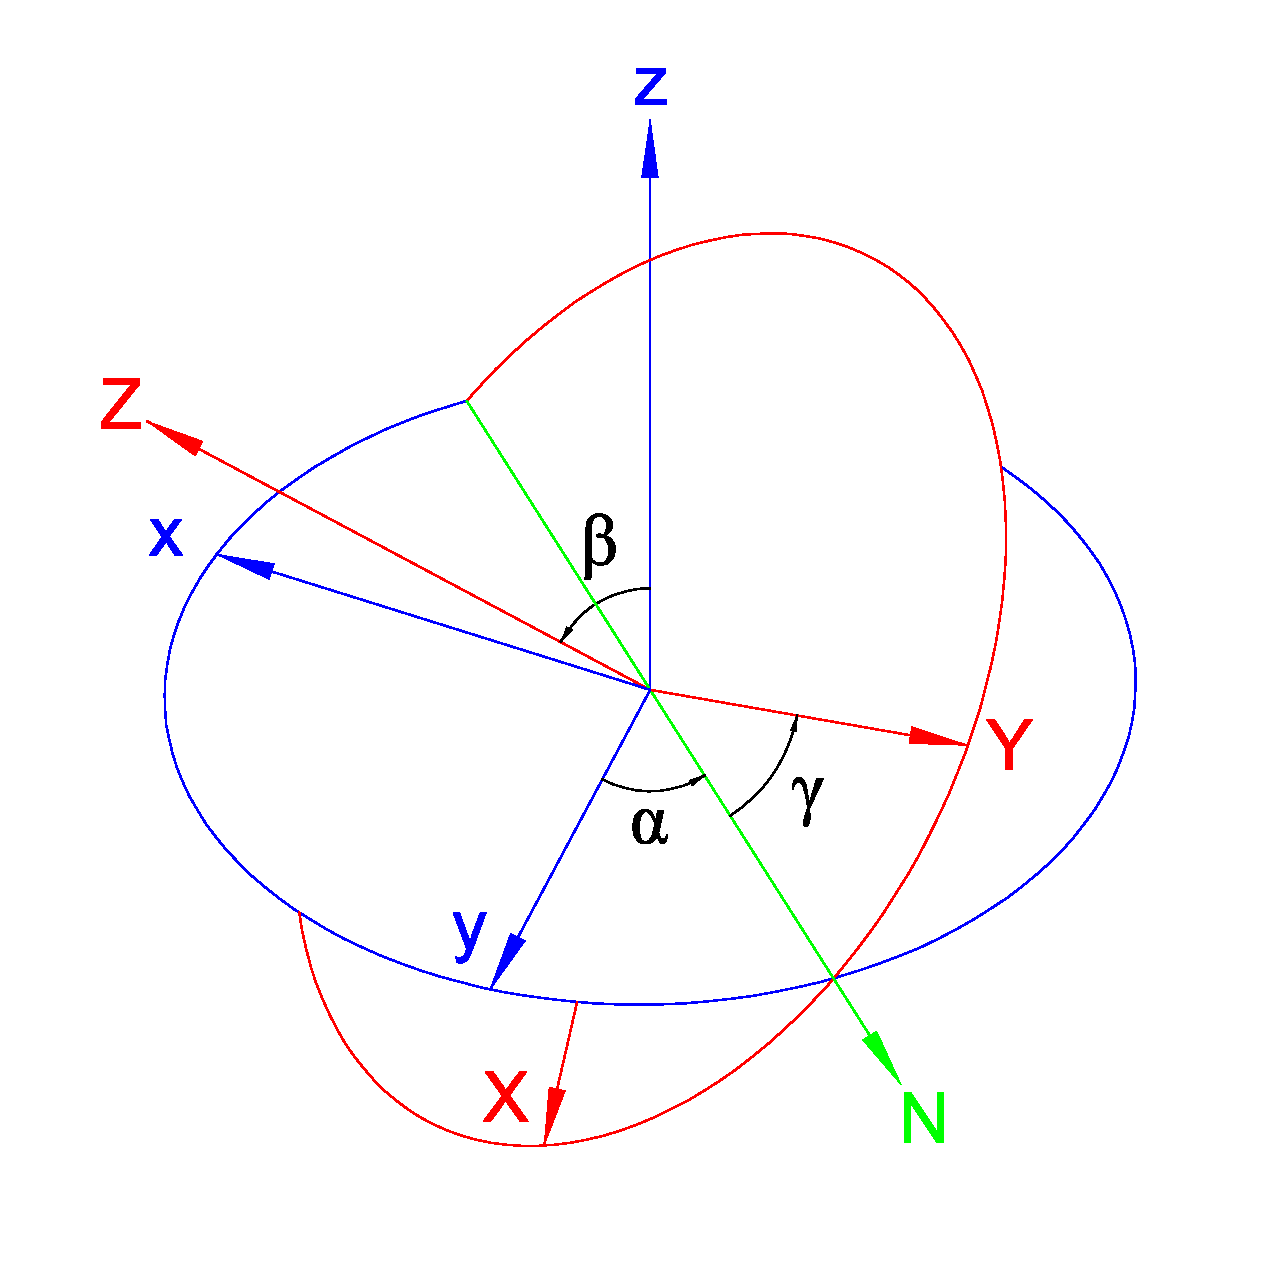
\includegraphics[width=7cm]{fig/ch13-eulerangleY.eps}
        \caption{欧拉角:临时轴$N$是$y$轴} \label{chlg:fig_euler}
    \end{minipage}
    \begin{minipage}[t]{0.49\textwidth}
        \centering
        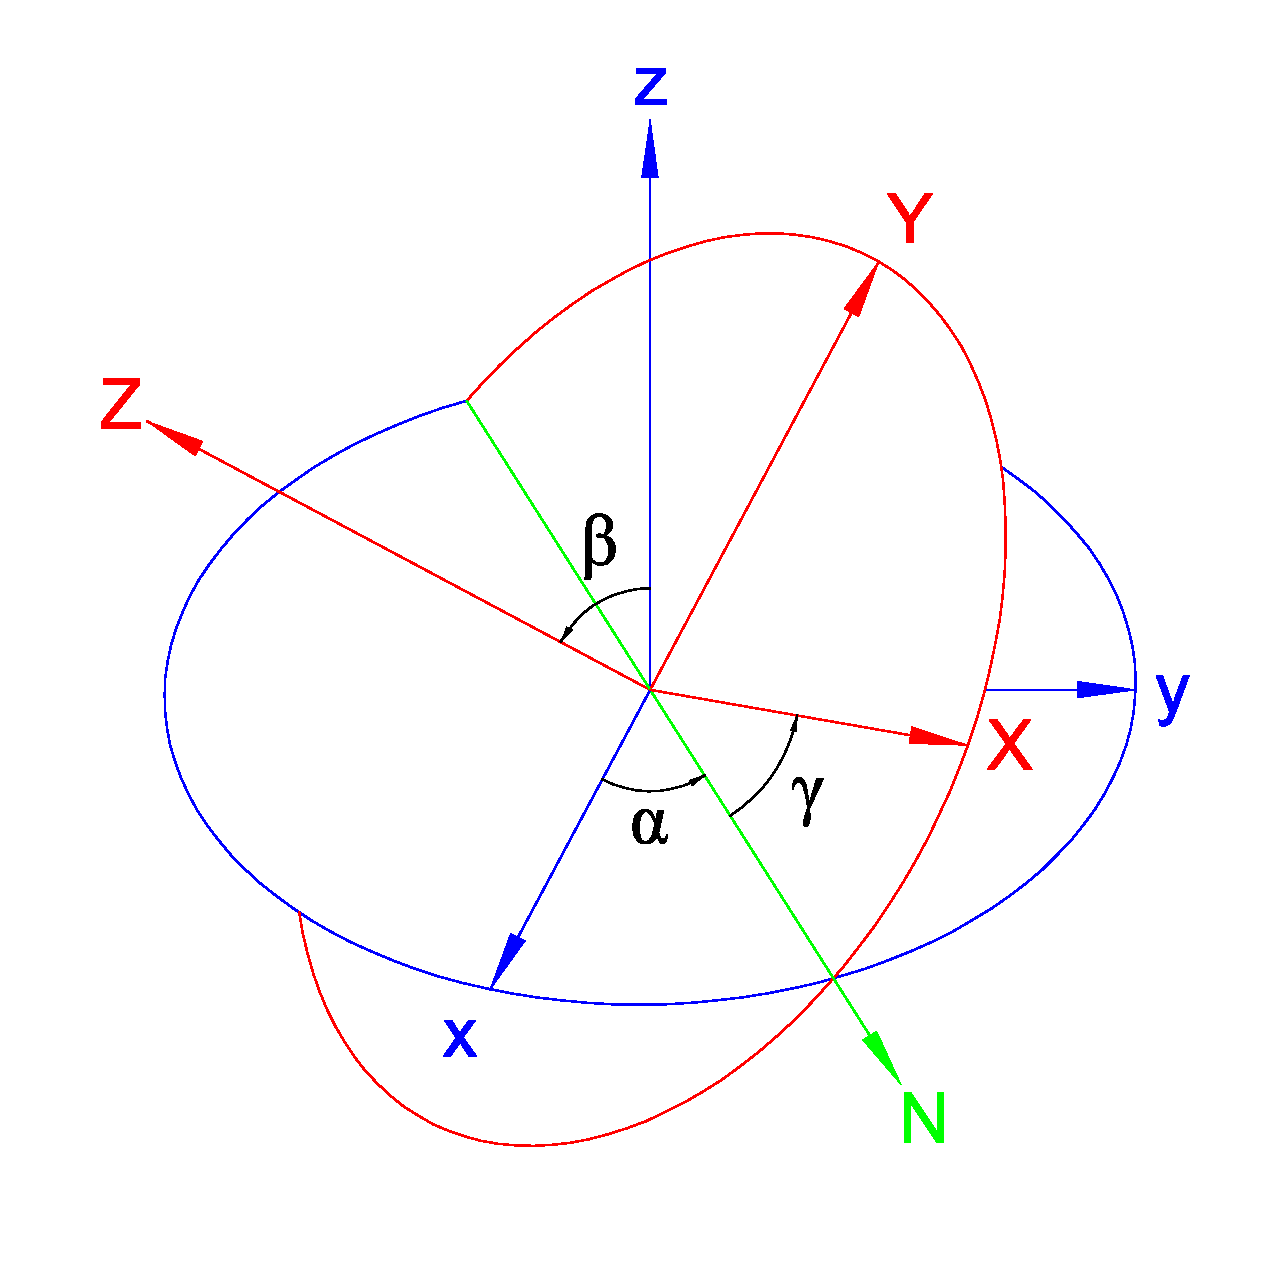
\includegraphics[width=7cm]{fig/ch13-eulerangleX.eps}
        \caption{欧拉角:临时轴$N$是$x$轴} \label{chlg:fig_euler2}
    \end{minipage}
\end{figure}


我们可以借用$\mathbb{R}^3$中常用的欧拉角$\alpha,\beta,\gamma$描述转动$R$.
图\ref{chlg:fig_euler}蓝色标小写字母$xyz$的坐标轴为
未转动的,红色标大写字母$XYZ$的坐标轴为
转动后最终位置,绿色标字母$N$的轴为中间步骤.
我们用$C_k(\psi)$表示绕$k$轴旋转$\psi$角.
第一步是进动,绕$z$轴转动$\alpha$角,即$C_z(\alpha)$,
转动后,$y$轴就转到了$N$轴位置,$z$轴不动.
第二步是章动{\footnote{章动英文是nutation,本意点头.地球除了进动(岁差),
        还有章动,周期大约18.6年.中国《周髀算经》中记载十九为一“章”,
        这就是此词翻译的由来($18.6\approx 19$).地球章动和天文观测光行差
        皆由英国人James Bradley(1693-1762)发现.}},
    绕$N$轴转动$\beta$角,即$C_N(\beta)$,
蓝色小写$z$轴转到了红色大写$Z$轴位置;蓝色的小写$xy$平面也
旋转到了红色大写$XY$平面.
第三步是自转,绕红色大写$Z$轴转动$\gamma$角,即$C_Z(\gamma)$,
此时就得到了坐标轴最终位置.我们将这三次转动记为
\begin{equation}\label{chlg:eqn_rotation}
    R(\alpha\beta\gamma)=C_Z(\gamma)C_N(\beta)C_z(\alpha) .
\end{equation}
注意转动的乘积顺序不能随意改变.%但这个表示不是很方便,需要进行化简.
我们注意到
\begin{align}
    C_N(\beta) &=C_z(\alpha)C_y(\beta)C_z(-\alpha) , \label{chlg:eqn_N_rotation} \\
    C_Z(\gamma)&=C_z(\alpha)C_y(\beta)C_z(\gamma)C_y(-\beta)C_z(-\alpha) . \label{chlg:eqn_Z_rotation}
\end{align}
代入上面的转动矩阵后,就得到了式\eqref{chlg:eqn_rotation}的欧拉角表示
\begin{small}
\setlength{\mathindent}{0em}
\begin{equation}\label{chlg:eqn_rotation_euler_y}
    \begin{aligned}
        &R(\alpha\beta\gamma)=C_z(\alpha)C_{\color{red}{y}}(\beta)C_z(\gamma) =   \\
        &\begin{pmatrix}
            \cos\alpha\cos\beta\cos\gamma -\sin\alpha \sin\gamma  &  -\cos\alpha \cos\beta \sin\gamma -\sin\alpha \cos\gamma & \cos\alpha \sin\beta  \\
            \sin\alpha\cos\beta\cos\gamma +\cos\alpha \sin\gamma  &  -\sin\alpha \cos\beta \sin\gamma +\cos\alpha \cos\gamma & \sin\alpha \sin\beta  \\
            -\sin\beta \cos\gamma & \sin\beta \sin\gamma & \cos\beta
        \end{pmatrix} .
    \end{aligned}
\end{equation}\setlength{\mathindent}{2em}
\end{small}
上面已经用到了绕坐标轴的旋转
\begin{equation}\label{chlg:eqn_rotation-zy}
    {C_z}( \alpha  ) =  \begin{pmatrix}
        {\cos \alpha }&{ - \sin \alpha }&0 \\
        {\sin \alpha }&{\cos \alpha }&0 \\
        0&0&1
    \end{pmatrix} ,\
    {C_y}( \beta ) = \begin{pmatrix}
        {\cos \beta }&0&{  \sin \beta }  \\
        0&1&0\\
        { - \sin \beta } &0&{\cos \beta }
    \end{pmatrix}  .
\end{equation}
图\ref{chlg:fig_euler}中临时轴$N$是$y$轴.
可将$N$选为$x$轴(图\ref{chlg:fig_euler2}),
此时式\eqref{chlg:eqn_rotation}为
\begin{small}
\setlength{\mathindent}{0em}
\begin{equation}\label{chlg:eqn_rotation_euler_x}
    \begin{aligned}
        &R(\alpha\beta\gamma)=C_z(\alpha)C_{\color{red}{x}}(\beta)C_z(\gamma) =   \\
        &\begin{pmatrix}
            \cos\alpha \cos\gamma-\sin\alpha \cos\beta \sin\gamma  & -\sin\alpha \cos\beta \cos\gamma -\cos\alpha \sin\gamma &  \sin\alpha \sin\beta \\
            \sin\alpha \cos\gamma+\cos\alpha \cos\beta \sin\gamma  &  \cos\alpha \cos\beta \cos\gamma -\sin\alpha \sin\gamma & -\cos\alpha \sin\beta \\
            \sin\beta  \sin\gamma & \sin\beta \cos\gamma  & \cos\beta
        \end{pmatrix} .
    \end{aligned}
\end{equation}\setlength{\mathindent}{2em}
\end{small}
其中
\begin{equation}\label{chlg:eqn_rotation-x}
    {C_x}( \beta  ) = \begin{pmatrix}
        1&0&0 \\
        0&{\cos \beta }&{ - \sin \beta } \\
        0&{\sin \beta }&{\cos \beta } \\
    \end{pmatrix} .
\end{equation}
两者没有本质差别.两种变换方法中,
欧拉角的取值范围是:$0 \leqslant \alpha, \gamma < 2\pi,\ 0\leqslant \beta \leqslant \pi$.
用欧拉角表示转动时,当$\beta=0$时,只要$\alpha+\gamma$的值相等就代表同一转动,有无穷多种表示;
同理,当$\beta=\pi$时,只要$\alpha-\gamma$的值相等就代表同一转动,有无穷多种表示;
这是需要注意的.这正反映了二维闭球面不能用一个坐标域覆盖的事实,即至少
需要两个坐标域才能覆盖二维球面流形.


式\eqref{chlg:eqn_rotation_euler_y}或式\eqref{chlg:eqn_rotation_euler_x}需
右作用在基矢量$\{\boldsymbol{e}_1,\boldsymbol{e}_2,\boldsymbol{e}_3\}$(行)上;
或者左作用在某矢量的具体分量$(x,y,z)^T$(列)上;不能反过来.

我们把$\mathfrak{so}(3)$李代数放到\S\ref{chlar:sec_LA-su2so3},与$\mathfrak{su}(2)$一起讨论.

\index[physwords]{广义正交群}  \index[physwords]{SO(p,q)}

\subsubsection{广义正交群}\label{chlg:sec_Opq}
在实数域$\mathbb{R}$中,取式\eqref{chlg:eqn_gsinit}中的$S$为
(按照物理习惯,作替换$S\to \eta$)
\begin{equation}\label{chlg:eqn_generalized-Lorentz-metric}
    \eta = \begin{pmatrix}
        -I_p & 0 \\  0 & I_q
    \end{pmatrix},
    \quad I_p,I_q \  \text{是单位矩阵};\
    p+q=m,\ 0\leqslant p,q\leqslant m .
\end{equation}
那么
\begin{equation}\label{chlg:eqn_gLorentz}
    O(p,q)=G(\eta)= \left\{ A \in GL(m,\mathbb{R})\ |\ A \eta {A}^T =\eta \right\},
\end{equation}
称为$(p,q)$型{\heiti 广义正交群}(Generalized orthogonal group);
当$p=1,q=3$时,就是通常的Lorentz群(见\S\ref{chlg:sec_Lorentz-group}).
不难发现$O(p,q)\cong O(q,p)$,两者只差一个相似变换.
有关系$O(m)\equiv O(0,m)$.
由式\eqref{chlg:eqn_gs}得它的李代数是
\begin{equation}\label{chlg:eqn_LA-opq}
    \mathfrak{o}(p,q)= \left\{ X \in 
    \mathfrak{gl}(m,\mathbb{R})\ |\  X\eta + \eta {X}^T =0 \right\}.
\end{equation}
通过上式可知它的维数是
\begin{equation}
    {\rm dim} \mathfrak{o}(p,q) = {\rm dim} O(p,q) = 
    \frac{1}{2}m(m-1)=\frac{1}{2}(p+q)(p+q-1).
\end{equation}

由式\eqref{chlg:eqn_gLorentz}可得广义正交矩阵行列式:
$ \det A \cdot\det\eta\cdot \det A^T = \det \eta \ \Rightarrow \ \det A = \pm 1$;
这也就注定了$O(p,q)$不是连通的.行列式为1的分支是
\begin{equation}\label{chlg:eqn_LG-sopq}
    SO(p,q)= \left\{ A \in GL(m,\mathbb{R})\ |\ A \eta {A}^T =\eta 
    \ \text{且}\ \det A = 1 \right\} .
\end{equation}
正交群$O(m)$有两个连通分支,而$O(p,q)$群有四个连通分支.将其记为
\begin{equation}
    g=\begin{pmatrix}
        a_T & b \\ c & a_S
    \end{pmatrix},
    \qquad \forall g\in O(p,q) ,\quad 0 < p < m.
\end{equation}
其中类时部分的$a_T$是$p\times p$的矩阵,类空部分的$a_S$是$q\times q$的矩阵.


可以用反证法证明它们的行列式都是非奇异的,即$|a_T| \neq 0$、$|a_S| \neq 0$.
假设行列式$|a_T| = 0$,则存在非零的$p$维列矢量$s$使得$a_T s =0$.
设$r=\binom{s}{0}$,则$gr=\binom{0}{cs}$.
首先,有$(gr)^T \eta gr = r^T (g^T \eta g) r = r^T \eta r = - s^T s <0 $;
其次,有$(gr)^T \eta gr = (0 \  cs) \eta \binom{0}{cs} = (cs)^T (cs)\geqslant 0$.
产生矛盾,故必有$|a_T| \neq 0$.类似可证$|a_S| \neq 0$.

对于$0 < p < m$的广义正交群可以分成四片,见表\ref{chlg:tab-GO}.

\begin{table}[htb]
    \centering
    \caption{$O(p,q)$群的分类记号} \label{chlg:tab-GO}
    \begin{tabular}{|*{4}{c|}}
        \hline 
        $| a_T| >0,\ | a_S |>0$ & $ |a_T| >0,\ | a_S |<0$ & $| a_T| <0,\ | a_S| >0$  & $| a_T| <0,\ | a_S| <0$ \\
        \hline
        $O^{++}(p,q)$ & $O^{+-}(p,q)$ & $O^{-+}(p,q)$ & $O^{--}(p,q)$   \\ 
        \hline
    \end{tabular}
\end{table}

不难发现:$SO(p,q)= O^{++}(p,q)\cup O^{--}(p,q)$.记$O^{++}(p,q)$为$SO^{+}(p,q)$.

当$0<p<m$时,$O(p,q)$及$SO^{+}(p,q)$是\uwave{非紧致的};这与正交群不同.

\index[physwords]{酉群}  \index[physwords]{SO$^{+}$(p,q)}  \index[physwords]{O$^{++}$(p,q)}

\subsubsection{酉群}\label{chlg:sec_unitary}

本节在在复数域$\mathbb{C}$中讨论问题.
此时,需要把式\eqref{chlg:eqn_gsinit}、\eqref{chlg:eqn_gs}中的一个矩阵换成
复共轭,即
\begin{align}
    G(S)=& \left\{ A \in GL(m,\mathbb{C})\ |\  A S \bar{A}^T =S \right\};\label{chlg:eqn_gsinit-cx} \\
    \mathfrak{g}(s) =& \left\{ X \in \mathfrak{gl}(m,\mathbb{C}) \ |\ 
    X S + S \bar{X}^T = 0 \right\} . \label{chlg:eqn_gs-cx}
\end{align}
请读者仿照本节开头论述一下上述构造仍是李群及其李代数.

取式\eqref{chlg:eqn_gsinit-cx}中的$S$为单位矩阵,那么
\begin{equation}\label{chlg:eqn_unitary}
    U(m)=G(S)= \left\{ A \in GL(m,\mathbb{C})\ |\ A \bar{A}^T =I \right\},
\end{equation}
称为{\heiti 酉群},也称为{\heiti 幺正群}
\footnote{Unitary group可以音译成 {\kaishu 酉群},常见于数学领域;
    也可以被意译成{\kaishu 幺正群},常见于物理领域.};
满足上式的复矩阵称为{\heiti 酉矩阵}或{\heiti 幺正矩阵}.
由式\eqref{chlg:eqn_gs-cx}得它的李代数是
\begin{equation}
    \mathfrak{u}(m)= \left\{ X \in 
    \mathfrak{gl}(m,\mathbb{C})\ |\ X  + \bar{X}^T =0 \right\}.
\end{equation}
通过上式可知$\mathfrak{u}(m)$的\uwave{实维数}是:$m^2$.
故酉群的李代数是由反厄米复矩阵组成.

可以证明$U(m)$群是紧致、连通的,故有$\exp \mathfrak{u}(m)= U(m)$.

设有幺正矩阵$U$,那么必然有$\bar{U}^T U = I$,两边取行列式,得
\begin{equation}
    1 = \det\bar{U}\cdot \det U =\overline{\det U} \cdot \det U
    \quad \Rightarrow \quad  \det U = e^{\mathbbm{i} \phi}, \ \phi\in \mathbb{R} .
\end{equation}
上式说明酉矩阵的行列式是模为一的复数,复角$\phi$无法确定,它处于复平面的单位圆周上.
如果进一步要求酉群元素的行列式为$+1$(复角$\phi=0$),那么可得{\heiti 特殊酉群},
\begin{equation}
    SU(m)= %U(m)\cap SL(m,\mathbb{C}) =
    \left\{ A \in GL(m,\mathbb{C})\ |\ A \bar{A}^T =I \ \text{且} \  \det A=1 \right\}.
\end{equation}
特殊酉群的李代数是零迹反厄米复矩阵
\begin{equation}\label{chlg:eqn_LA-su}
    \mathfrak{su}(m) %= \mathfrak{u}(m)\cap \mathfrak{sl}(m,\mathbb{C}) 
    =\left\{X\in\mathfrak{gl}(m,\mathbb{C})\ |\ X+\bar{X}^T=0
    \ \text{且} \  {\rm Tr} X =0 \right\} .
\end{equation}
$\mathfrak{su}(m)$的\uwave{实维数}是:$m^2-1$.


可以证明$SU(m)$是紧致、单连通的李群,
故有$\exp \mathfrak{su}(m) = SU(m)$.

\index[physwords]{U(1)群}

\paragraph{$U(1)$群}
此时式\eqref{chlg:eqn_unitary}中的矩阵$A$是一维的,
可设$[A]=a+\mathbbm{i} b$(其中$a,b\in \mathbb{R}$),
那么有$a^2+b^2=1$;由此可见$U(1)$与$SO(2)$群同构.
很明显,$U(1)$还能表示成指数形式:
$U(1)=\exp (\mathbbm{i}\theta),\ \theta\in \mathbb{R}$.
$U(1)$是连通的,但不是单连通的.

$SU(1)$不是连续群,是单点集($(1,0)$),平庸无奇.

%在\S\ref{chlar:sec_SU2SO3}将具体讲解$SU(2)$群.

%$U(1)$是一维李群,容易求得一维反厄米矩阵是由虚数单位“$\mathbbm{i}$”构成的线性空间;

\index[physwords]{辛群}

\subsubsection{辛群}
在数域$\mathbb{F}$中,取式\eqref{chlg:eqn_gsinit}中的$S$为反对称矩阵
\begin{equation}
    J = \begin{pmatrix}
            0 & I_m \\ -I_m & 0
        \end{pmatrix},
\end{equation}
那么
\begin{equation}
    Sp(m,\mathbb{F})=G(J)= \left\{ A \in GL(2m,\mathbb{F})\ |\ A J {A}^T =J \right\},
\end{equation}
称为{\heiti 辛群}(Sympletic group),
$Sp(m,\mathbb{F})$中的元素称为{\heiti 辛矩阵}.
它的李代数是
\begin{equation}
    \mathfrak{sp}(m,\mathbb{F})= \left\{ X \in 
    \mathfrak{gl}(2m,\mathbb{F})\ |\ X J + J {X}^T =0 \right\}.
\end{equation}
由上式可得复辛群的\uwave{实维数}是 $2(2m^2+m)$,实辛群维数是 $2m^2+m$.

%$Sp(m,\mathbb{F})$是连通的(点集拓扑);非紧致的.代数拓扑连通属性是:复辛群是单连通,实辛群是$\infty$度连通.



\begin{table}[htb]
    \centering
    \caption{常用矩阵李群} \label{chlg:tab_groups}
    \begin{tabular}{|*6{c|}}
        \hline
        李群 &矩阵 & 实维数 &连通性  & 紧致性 & 李群李代数   \\        \hline
        $GL(m,\mathbb{R})$ & $m$维可逆实矩阵 & $m^2$  & \makecell{非连通\\非单连通 }
        & 非紧 & \makecell{$m$维任意\\ 实矩阵}   \\ \hline
        $GL(m,\mathbb{C})$& $m$维可逆复矩阵 & $2 m^2$ & \makecell{连通 \\非单连通 }
        & 非紧 & \makecell{$m$维任意\\ 复矩阵}  \\ \hline
        $SL(m,\mathbb{R})$ & \makecell{行列式为$1$的\\$m$维可逆实矩阵} & $m^2-1$  &  \makecell{连通 \\ 非单连通 } 
        & 非紧 & \makecell{$m$维无迹\\ 实矩阵}  \\ \hline
        $SL(m,\mathbb{C})$ & \makecell{行列式为$1$的\\$m$维可逆复矩阵} & $2m^2-2$ & \makecell{连通\\单连通 }
        & 非紧 & \makecell{$m$维无迹\\ 复矩阵}  \\ \hline
        $O(m)$  & $m$维正交实矩阵 & $\dfrac{m(m-1)}{2}$  & \makecell{非连通\\非单连通 } 
        & 紧致 & \makecell{$m$维反对\\ 称实矩阵} \\ \hline
        $SO(m)$ & \makecell{行列式为$1$的\\$m$维正交实矩阵} &$\dfrac{m(m-1)}{2}$ & \makecell{连通\\2度连通 }
        & 紧致 & \makecell{$m$维反对\\ 称实矩阵}  \\ \hline
        $SO^{+}(1,3)$ & \makecell{$4$维实矩阵$\Lambda$\\且$\eta=\Lambda^T \eta \Lambda$} & $6$ & \makecell{连通\\2度连通 }
        & 非紧 & \makecell{$4$维实矩阵$A$\\$A^T=- \eta A \eta $} \\ \hline
        $U(m)$ & $m$维幺正矩阵 & $m^2$ & \makecell{连通 \\$\infty$度连通 }
        & 紧致 &  \makecell{$m$维反厄\\ 米复矩阵} \\ \hline
        $SU(m)$ & \makecell{行列式为$1$的\\$m$维幺正矩阵} & $m^2-1$ & \makecell{连通\\单连通 }
        & 紧致 & \makecell{$m$维反厄米\\无迹复矩阵} \\ \hline
    \end{tabular}
\end{table}

{\kaishu 表\ref{chlg:tab_groups}中“连通性”一栏,上面是点集拓扑的连通属性;
下面是代数拓扑的属性(单连通或复连通).表中“维数”是指实数域上李群的维数.}



\subsection{古典李群、李代数}\label{chlg:sec_clg}
\index[physwords]{古典李群}  \index[physwords]{古典李代数}

记$A_m$为$SL(m+1,\mathbb{C})$.记$C_m$为$Sp(m,\mathbb{C})$.

在复数域$\mathbb{C}$中,取式\eqref{chlg:eqn_gsinit}中的$S$为单位矩阵$I$,则
\begin{equation*}
    O(m,\mathbb{C}) = \left\{ A \in GL(m,\mathbb{C})\ |\ A A^T =I \right\};
    \quad SO(m,\mathbb{C}) = O(m,\mathbb{C}) \cap SL(m,\mathbb{C}).
\end{equation*}
记$B_m$为$SO(2m+1,\mathbb{C})$.记$D_m$为$SO(2m,\mathbb{C})$.

$A_m$、$B_m$、$C_m$、$D_m$称为{\heiti 古典李群},其李代数称为{\heiti 古典李代数}.

复数域上的正交群$O(m,\mathbb{C})$在物理学上几乎无用,同时我们不省略复数域$\mathbb{C}$的标记.
本书中,所有的$O(m)$均指$O(m,\mathbb{R})$,即省略实数域$\mathbb{R}$的标记.

%\begin{proposition}
%    {\bfseries (1)}:$\bigl( \mathfrak{so}(m,\mathbb{R})\bigr)^{\mathbb{C}}=\mathfrak{so}(m,\mathbb{C})$.    
%    {\bfseries (2)}:$\bigl( \mathfrak{sl}(m,\mathbb{R})\bigr)^{\mathbb{C}}=\mathfrak{sl}(m,\mathbb{C})$.    
%    {\bfseries (3)}:$\bigl( \mathfrak{sp}(m,\mathbb{R})\bigr)^{\mathbb{C}}=\mathfrak{sp}(m,\mathbb{C})$.    
%    {\bfseries (4)}:$\mathfrak{su}(m,\mathbb{C})$是$\mathfrak{sl}(m,\mathbb{C})$的实形式.
%\end{proposition}
%\begin{proof}
%    前三条几乎一望而知.下面证明第(4)条,需要提醒一下,$\mathfrak{su}(m)$本来就定义在
%    复数域上,没有$\mathfrak{su}(m,\mathbb{R})$.
%\end{proof}

\begin{theorem}\label{chlg:thm_CLA-simple}
    古典李代数$A_m(m\geqslant 1)$、$B_m(m\geqslant 1)$、$C_m(m\geqslant 1)$、$D_m(m\geqslant 3)$是
    单纯李代数.(证明见\parencite[p.148]{huangxg-2024}定理6,或\parencite[\S 1.3]{wanzx-2013}定理1.2)
\end{theorem}







\section{物理中常用等距李群}\label{chlg:sec_matrixG-II}
继\S\ref{chlg:sec_isometry},本节再描述一些保度规群\cite{tung-1985},有些群会涉及流形局部坐标.


\subsection{等距映射补遗}\label{chlg:sec_iso-add}
在\S \ref{chrg:sec_isometry}我们已初步讨论了等距映射(Isometry),
等距定义自然仍为\ref{chrg:def_isometry-immersion};我们从群论角度再次讨论这个问题.

\index[physwords]{等距群}
\index[physwords]{I(M)|see{等距群}}

对于光滑广义黎曼流形$M$,所有从$M$到$M$的等距映射集合$I(M)$,在把
复合映射当成群乘法的情形下构成一个群,称为$M$的{\heiti 等距群}.
验证$I(M)$是群的工作留给读者(极易).粗略地说,$I(M)$越大,$M$越简单.
有的$M$除了恒等映射之外可能没有等距映射,称为平凡情形;
但是许多流形有足够大的等距群,因此可以应用李群知识.
在非平凡情况下,$I(M)$是$M$的几何不变量,它的重要性几乎可以和曲率、测地线比拟.

由于$M$的每个切空间与$\mathbb{R}^n_\nu$是(局部)等距同胚的,
因此等距群$I(\mathbb{R}^n_\nu)$在广义黎曼几何中具有基本意义.
%特别是,对于具有不定度规的流形,它导致了类似于普通可定向性的时间和空间可定向性的孪生概念.

\begin{theorem}\label{chlg:thm_isoexp}
    设在广义黎曼流形$(M,g)$、$(N,h)$间存在局部等距同构映射$\phi:M\to N$.
    则$\forall p\in M$,交换图\ref{chlg:pic_exp-exchange}成立;
    其中$U_p\subset T_pM$,$V_{\phi(p)}\subset T_{\phi(p)}N$分别
    是$\exp_p$和$\exp_{\phi(p)}$的法邻域(指数映射的像集,见\S\ref{chgd:sec_exp}).
\end{theorem}

\begin{figure}[htb]
    \centering
    \begin{tikzpicture}[scale=5]
        \draw[thick] [-latex] (0,0)node[left]{$U_p$}--(0.5,0)node[below]{$\phi_*$}   --(1,0) node[right] {$V_{\phi(p)} $};
        \draw[thick] [-latex] (-0.05,-0.05) -- (-0.05,-0.2)node[left] {$\exp_p$}   --(-0.05,-0.4)node[below ] {$M$};
        \draw[thick] [-latex] (1.05,-0.05) -- (1.05,-0.2)node[right]{$\exp_{\phi(p)}$}   --(1.05,-0.4)node[below ] {$N$};
        \draw[thick] [-latex] (0,-0.55)--(0.5,-0.55)node[above]{$\phi$} --(1,-0.55) ;
    \end{tikzpicture}
    \caption{等距——指数映射交换图}\label{chlg:pic_exp-exchange}
\end{figure}

\begin{proof}
    设$\gamma(t)$是$M$中测地线,且$p=\gamma(0)$;由定理\ref{chrg:thm_geodesic-MN}可知
    映射$\phi\circ\gamma(t)$是$N$中测地线.
    $\forall v\in U_p$,与之对应$\phi_* v \in V_{\phi(p)}$;两条测地线诱导的指数映射分别是:
    $\exp_p(t v)=\gamma(t;p,v)$和
    $\exp_{\phi(p)}(t\, \phi_*v)=\phi\circ\gamma\bigl(t;\phi(p),\phi_* v\bigr)$.
    由定理\ref{chrg:thm_geodesic-MN}有
    \begin{equation}\label{chlg:eqn_isoexp}
        \phi \bigl(\exp_p(t v)\bigr) = \exp_{\phi(p)}(t\, \phi_* v ) .
    \end{equation}
    这正是本定理需要证明的,即交换图\ref{chlg:pic_exp-exchange}.
\end{proof}

%\parencite{oneill1983}定理3.62
\begin{proposition}\label{chlg:thm_isopall}
    设有两个连通广义黎曼流形$M$、$N$,存在局部等距同构映射$\phi,\psi:M\to N$.
    若存在一个点$p\in M$使得$\phi(p)=\psi(p)$和$\phi_{p*} = \psi_{p*}$成立,
    则有$\phi=\psi$.
\end{proposition}
\begin{proof}
    令$A=\{ q\in M \ | \  \phi_{q*} = \psi_{q*}\}$.因$p\in A$,故$A$不是空集;
    又因映射的连续性可知$A$不只包含$p$点.    $\forall q\in A$,
    自然存在$q$的法邻域$U\subset M$;
    那么$\forall r\in U$一定存在$v\in T_q M$使得$r=\gamma_v(1)=\exp_q(v)$成立;
    则(要用式\eqref{chlg:eqn_isoexp})
    \begin{equation}
        \phi(r) = \phi \bigl(\gamma_v(1)\bigr)= \gamma_{\phi_*(v)} (1)
        = \gamma_{\psi_*(v)} (1) =\psi \bigl(\gamma_v(1)\bigr) =\psi(r).
    \end{equation}
    故在开集$U$上$\phi=\psi$;
    因此$\forall r\in U$,都有$\phi_{r*} = \psi_{r*}$;从而$U\subset A$;
    这说明$A$是$M$中的开集.如果$A$不能覆盖整个$M$,那么
    另取$w\in A$且$w\neq p$,以$w$为原点再次运用指数映射方式将$A$延拓,
    直至能够覆盖流形$M$.
\end{proof}

\begin{example}\label{chlg:exam_DQpsi}
    标量函数场变换规则.
\end{example}      
我们以量子物理中的波函数为例来说明标量函数场在对称操作下的变换规则.
考虑量子物理中一个态矢量$|\psi\rangle$,在位型空间表象中态函数
是$\psi(\boldsymbol{r}) = \langle \boldsymbol{r}|\psi\rangle$.
用$Q$表示某种对称作用,它会把态函数作整体变换;
变换后在新的位置$\boldsymbol{r}'=Q \boldsymbol{r}$的态函数与老位置的态函数是
相等的,这是对称变换的要求;用公式表示为
\begin{equation}
    \psi(\boldsymbol{r}) = \psi'(\boldsymbol{r}')
\end{equation}
我们将新旧位置关系($\boldsymbol{r}'=Q \boldsymbol{r}$)带入上式,有
\begin{equation}
    \psi(\boldsymbol{r}) = \psi'(Q \boldsymbol{r}) \quad \Leftrightarrow \quad
    \psi(Q^{-1}\boldsymbol{r}) = \psi'(\boldsymbol{r}) .
\end{equation}
在对称变换$Q$的作用下,新的态矢量$\psi'$可用一个函数变换算符来表示,即
\begin{equation}\label{chlg:eqn_psip2psi}
    \psi'(\boldsymbol{r}) \overset{def}{=}\hat{D}(Q)\psi(\boldsymbol{r}).
    \qquad \text{等号两边的宗量$\boldsymbol{r}$是相同的}
\end{equation}
那么便有
\begin{equation}\label{chlg:eqn_DQpsi}
    \psi(Q^{-1}\boldsymbol{r})  = \psi'(\boldsymbol{r}) \equiv \hat{D}(Q)\psi(\boldsymbol{r}) .
\end{equation}
上式便是态矢量在对称变换下的变化关系式.    \qed


\index[physwords]{平移群}

\subsection{平移群}\label{chlg:sec_translation-group}
在$\mathbb{R}^m$中,{\heiti 平移}(translation)是一种几何变换,
它将图形、形状或空间的每个点在给定方向上移动相同的距离.
平移也可以解释为向每个点添加一个常量矢量,或移动坐标系的原点.
用坐标语言来说,便是:
\begin{equation}\label{chlg:eqn_translation}
    x\to x' : x'^{i} = x^i + a^i 
    \quad \Leftrightarrow \quad
    \boldsymbol{x}' =\hat{Q}(\boldsymbol{x})= \boldsymbol{x} + \boldsymbol{a} ;
    \qquad 1 \leqslant i \leqslant m .
\end{equation}
其中$x^i$是旧坐标,$x'^i$是新坐标,$a^i$是常数.
需要强调一点:算符$\hat{Q}$不是线性算符,
例如$\hat{Q} (2 \boldsymbol{x}) =2 \boldsymbol{x} + \boldsymbol{a} \neq 
2\bigl(\hat{Q}(\boldsymbol{x})\bigr)=2 \boldsymbol{x} + 2\boldsymbol{a}$.

仅有平移的坐标表示是不够的,假设存在用坐标$\{x^i\}$描述的
标量函数$f(\boldsymbol{x})$,我们要求$f(\boldsymbol{x})$在平移操作下不变;
参考式\eqref{chlg:eqn_DQpsi},用$\hat{T}(m)$表示作用在$f$上的算符,有
\begin{equation}\label{chlg:eqn_translationONf}
    f'(\boldsymbol{x})=\hat{T}(m) f(\boldsymbol{x})= f(\hat{Q}^{-1}\boldsymbol{x}) = f(\boldsymbol{x} - \boldsymbol{a}) .
\end{equation}


自然把群乘法取成连续进行两次“坐标加法”,
即$\boldsymbol{x}$加上$\boldsymbol{b}$,再加上$\boldsymbol{a}$;
对于$\hat{T}(m)$来说便是复合映射,即群乘法是
\begin{equation*}
    \hat{T}(m)_{\boldsymbol{a}}\circ \hat{T}(m)_{\boldsymbol{b}}\ f(\boldsymbol{x}) 
    = \hat{T}(m)_{\boldsymbol{a}}\ f(\boldsymbol{x} - \boldsymbol{b}) 
    = f(\boldsymbol{x} - \boldsymbol{b} - \boldsymbol{a}) 
    = \hat{T}(m)_{\boldsymbol{b}+ \boldsymbol{a}}\ f(\boldsymbol{x}) .
\end{equation*}
容易验证上式操作构成群:
首先,此操作具有封闭性;其次,加法具有结合性;
第三,当$\boldsymbol{a}=0$时,操作\eqref{chlg:eqn_translationONf}是恒等映射,可看作单位元;
最后,参量是$-\boldsymbol{a}$和$+\boldsymbol{a}$的操作互逆.
由于加法具有交换性(即群乘法具有交换性),故此群是可对易群(阿贝尔群);
我们称之为{\heiti 平移群}.
由于$\mathbb{R}^m$本身就是光滑流形,再加上“群乘法”和“求逆”运算是$C^\infty$的
(加法和取负号操作当然是$C^\infty$的),故\uwave{平移群是李群}.

平移群适用于各种度规场,但我们只考虑正定度规以及闵氏度规.

由于李群是可微的,我们将式\eqref{chlg:eqn_translationONf}展开,有
\begin{equation*}
    \hat{T}(m) f(\boldsymbol{x}) = f(\boldsymbol{x} - \boldsymbol{a}) 
    = f(\boldsymbol{x}) + (-a^i) \frac{\partial f(\boldsymbol{x})}{\partial x^i}
    +\frac{1}{2!} (-a^i)(-a^j) \frac{\partial^2 f(\boldsymbol{x})}{\partial x^i \partial x^j}
    +\cdots 
\end{equation*}
上式说明,平移算符可以表示成
\begin{equation}\label{chlg:eqn_Texp}
    \hat{T}(m) \equiv \exp\left( -a^j \frac{\partial }{\partial x^j} \right) 
    \equiv\exp\left(-\mathbbm{i} a^j \hat{P}_j  \right) , \qquad
    \hat{P}_j\overset{def}{=} -\mathbbm{i}\frac{\partial }{\partial x^j} .
\end{equation}
上式中顺便给出了平移$\hat{P}_j$的定义;
并且把平移算符形式地表示成指数形式.
由于两个不同坐标的偏导数是可交换的,所以不难看出式\eqref{chlg:eqn_Texp}中的
平移算符仍是阿贝尔群.
上面给出的平移算符是微分形式的,在式\eqref{chlg:eqn_Trans-Momen}中给出了平移李代数
的矩阵形式.

虽然算符$\hat{Q}$不是线性算符,但平移算符$\hat{T}(m)$是线性的,例如
\begin{equation*}
    \hat{T}(m) \bigl(2f(\boldsymbol{x})\bigr) 
    =2\left( f(\boldsymbol{x}) - a^i \frac{\partial f(\boldsymbol{x})}{\partial x^i}
    +\frac{1}{2!} a^i a^j \frac{\partial^2 f(\boldsymbol{x})}{\partial x^i \partial x^j}
    +\cdots \right) = 2 f(\boldsymbol{x}) .
\end{equation*}

平移群是连通、单连通、非紧致李群.

\begin{example}\label{chlg:exam_pm2}
    号差为$-2$的Lorentz度规下的平移算符.
\end{example}
号差为$+2$的Lorentz度规下动量算符定义成$\hat{P}_\mu =- \mathbbm{i}\frac{\partial }{\partial x^\mu}$
(见式\eqref{chlg:eqn_Texp}),有一个负号;同时非时间部分$\hat{P}_j =\hat{P}^j$(即$j=1,2,3$),
时间部分$\hat{P}_0 =-\hat{P}^0$.

不论何种号差,逆变矢量的形式是一样的;故不论号差,动量算符的逆变形式为:
$\hat{P}^\mu=\mathbbm{i}\{\frac{\partial}{\partial t}, -\frac{\partial}{\partial x},
-\frac{\partial}{\partial y},-\frac{\partial}{\partial z}\}$.
由此可知号差为$-2$的Lorentz度规下动量算符是:
$\hat{P}^\mu = \mathbbm{i}\frac{\partial }{\partial x_\mu}$以及
$\hat{P}_\mu = \mathbbm{i}\frac{\partial }{\partial x^\mu}$.

除此以外,在不同号差下,两个矢量的缩并也相差一个负号;故号差为$-2$的Lorentz度规下平移
算符是$\hat{T}(m) = \exp\left(\mathbbm{i} a^\mu \hat{P}_\mu  \right) $,
与式\eqref{chlg:eqn_Texp}差一负号.\qed


\index[physwords]{欧几里得群}

\subsection{欧几里得群}\label{chlg:sec_Euclidean-group}
在低速、低能情形下(比如牛顿力学范畴内),几乎所有证据表明,
三维物理空间是均匀和各向同性的,因此在孤立系统上进行的科学实验的结果
不应取决于所使用的实验装置(或参考系)的特定位置或方向.
这一基本事实是通过假设基础空间是一个欧几里得空间而纳入数学框架的.
$m$维欧几里得空间(正定度规)的对称群是欧几里得群(记为$E(m)$或$ISO(m)$):
\begin{definition}
    欧几里得群由$(\mathbb{R}^m,\delta)$上的所有连续、等距、“线性”变换组成.
\end{definition}
上述定义中线性两个字加上引号是因为平移不是线性算符(见\S\ref{chlg:sec_translation-group}),
纯旋转是线性算符;无穷小平移是线性的.对应的坐标变换是
\begin{equation}\label{chlg:eqn_trans-rot}
    x\to x' : x'^{i} = R^i_{\cdot j}x^j + a^i ,\qquad  1 \leqslant i \leqslant m .
\end{equation}
用矩阵形式表示为(后面会证明式中$R\in O(m)$)
\begin{equation}\label{chlg:eqn_Em-max}
    \begin{bmatrix}  \boldsymbol{x}' \\ 1 \end{bmatrix} =
    \begin{bmatrix}  R & \boldsymbol{a} \\ \boldsymbol{0}^T & 1  \end{bmatrix}
    \begin{bmatrix}  \boldsymbol{x} \\ 1 \end{bmatrix} 
    \  \overset{def}{=} \boldsymbol{T} \begin{bmatrix}  \boldsymbol{x} \\ 1 \end{bmatrix} .
    \qquad \boldsymbol{T}^{-1} = 
    \begin{bmatrix}    R^{-1} & -R^{-1} \boldsymbol{a} \\ \boldsymbol{0}^T & 1    \end{bmatrix} .
\end{equation}
我们把一个$m$维列矢量末尾增加一行,数值为$1$;从而变成了$m+1$维列矢量,
称之为{\heiti 齐次坐标};这样做的目的只是为了表示方便,没有其它意义了.
上式最后定义了矩阵$\boldsymbol{T}$,并给出了它的逆.

在空间均匀前提下,平移(见\S\ref{chlg:sec_translation-group})是等距变换,
这种性质与度规是否正定无关.在正定度规下,要求此变换是等距的,即
\begin{align*}
    (x'-y')^T (x'-y') = ( \boldsymbol{x} - \boldsymbol{y} )^T R^T  R ( \boldsymbol{x} - \boldsymbol{y} )
    = (x-y)^T (x-y) \ \Rightarrow\ R^T R = I .
\end{align*}
可见只要变换$R$是实正交矩阵(见\S\ref{chlg:sec_Orthogonal})就可等距,
也就是$R$是$O(m)$群中的元素,包含纯转动和反射.
这便说明了欧几里得群由两种类型的变换组成:平移和转动.
为了使问题简化,可以将$R$限定在$SO(m)$中;
此时,通常把$E(m)$记为$SE(m)$或$E^+ (m)$.

这就是说$I(\mathbb{R}^m)=E(m)$,它的维数是:
\begin{equation*}
    {\rm dim}\bigl(I(\mathbb{R}^m)\bigr)= {\rm dim}  \hat{T}(m) + {\rm dim} O(m)
    = m + m(m-1)/2 = m(m+1)/2 .
\end{equation*}



%由于$\hat{T}(m)$和$R(\theta)$通常情形下是不对易的,因此$E(m)$以非平凡的方式将它们组合起来.
我们把$E(m)$的群乘法定义为复合映射,连续两次欧氏变换为
\begin{small}
\setlength{\mathindent}{0em}
\begin{equation}\label{chlg:eqn_Emtimes}
    \begin{bmatrix}  R_1 & \boldsymbol{a_1} \\ \boldsymbol{0}^T & 1  \end{bmatrix}
    \begin{bmatrix}  R_2 & \boldsymbol{a_2} \\ \boldsymbol{0}^T & 1  \end{bmatrix}
    \begin{bmatrix}  \boldsymbol{x} \\ 1 \end{bmatrix} 
    =\begin{bmatrix}  R_1 & \boldsymbol{a_1} \\ \boldsymbol{0}^T & 1  \end{bmatrix}
    \begin{bmatrix}  R_2\boldsymbol{x} + \boldsymbol{a_2} \\  1  \end{bmatrix}
    =\begin{bmatrix}  R_1 R_2\boldsymbol{x} + R_1 \boldsymbol{a_2} +\boldsymbol{a_1} \\  1  \end{bmatrix}.
\end{equation}\setlength{\mathindent}{2em}
\end{small}
很明显,两次欧氏变换是不可对易的.
不难验证平移群$\hat{T}(m)$是$E(m)$的\uwave{不变子群},
即$\forall u \in E(m)$,$\forall t \in \hat{T}(m)$有
\begin{equation}
    u^{-1} t u x= 
    \begin{bmatrix}  R^{-1} & -R^{-1} \boldsymbol{a} \\ \boldsymbol{0}^T & 1    \end{bmatrix}
    \begin{bmatrix}  R\boldsymbol{x} + \boldsymbol{a} +  \boldsymbol{t}\\  1  \end{bmatrix}
    =\begin{bmatrix} \boldsymbol{x} + R^{-1} \boldsymbol{t}\\  1  \end{bmatrix}.
\end{equation}
因为$E(m)$有一个不变子群$\hat{T}(m)$,所以它不是一个单纯群;因为$\hat{T}(m)$
是阿贝尔的,故它也不是半单纯的.
$E(m)$是不连通的,它有两个分支;其中$SE(m)$是包含单位元的连通分支.
因平移群是非紧致的,故$E(m)$也是非紧致李群.

依照\S\ref{chlg:sec_semi-dir-prod}可知:$E(m)= \hat{T}(m) \rtimes O(m)$.
依照半直积定义可以把$E(m)$中元素记为$(t,o)$,其中$t\in \hat{T}(m)$,
$o\in O(m)$,且不能把$(t,o)$改变顺序为$(o,t)$.
为了更清晰地描述这个半直积,我们从定义的角度再次描述一下.
可以定义平移群$\hat{T}(m)$的自同构映射为:
$\Psi_{R_1}( \boldsymbol{a}_2)=R_1 \boldsymbol{a}_2 = \hat{T}(m)_{R_1 \boldsymbol{a}_2}$,
其中$R_1 \in O(m)$,$\boldsymbol{a}_2\in \hat{T}(m)$.
那么连续两次欧氏变换可以表示为:
$(\boldsymbol{a}_1, R_1)(\boldsymbol{a}_2, R_2)=(\boldsymbol{a}_1 \Psi_{R_1}( \boldsymbol{a}_2), R_1 R_2)
=(\boldsymbol{a}_1 + R_1 \boldsymbol{a}_2 , R_1 R_2)$.
这与上面用矩阵表示的连续两次欧氏变换完全相同.



%下面稍微介绍一下最简单的欧氏群:$ISO(2)$(Inhomogeneous SO).

\index[physwords]{ISO(2)群}

\subsubsection{$ISO(2)$}\label{chlg:sec_e2}
二维欧几里得群$ISO(2)$(或$E(2)$)的乘法关系\eqref{chlg:eqn_Em-max}中的$\boldsymbol{T}$可表示为
\begin{equation}
    \boldsymbol{T}( \boldsymbol{a}, \theta ) =  \begin{pmatrix}
        {\cos \theta }&{ - \sin \theta }& a^1 \\
        {\sin \theta }&{\cos \theta }& a^2 \\
        0&0&1
    \end{pmatrix} .
\end{equation}
很明显,$\boldsymbol{T}( 0, \theta )$是$SO(2)$,它表示$x-y$平面内的旋转(即绕$z$轴旋转),
它可以表示成(参见式\eqref{chlar:eqn_expSO3})
\begin{equation}\label{chlg:eqn_tmpR}
    \boldsymbol{T}( 0, \theta )= R(\theta ) =\exp(-\mathbbm{i} \theta J); \
    J = \left(\begin{smallmatrix}
        0 & -\mathbbm{i} & 0 \\
        \mathbbm{i} & 0 & 0 \\
        0 & 0 & 0
    \end{smallmatrix} \right)\cong
    \hat{J} = -\mathbbm{i} (x \partial_y - y \partial_x ).
\end{equation}
$\boldsymbol{T}( \boldsymbol{a}, 0 )$是平移群$\hat{T}(2)$.
在李代数同构前提下,李代数基矢是矩阵还是偏导数算符是没有差别的.
平移群算符\eqref{chlg:eqn_Texp}中使用的是偏导数算符,
现把它换成矩阵形式(参考\eqref{chlg:eqn_Em-max}):
\begin{small}
\begin{equation}\label{chlg:eqn_Trans-Momen}
    \hat{P}_1 = -\mathbbm{i}\frac{\partial }{\partial x^1}  \ \cong \  
    \begin{pmatrix}
        0 & 0 & \mathbbm{i} \\
        0 & 0 & 0 \\
        0 & 0 & 0
    \end{pmatrix}\equiv P_1,\quad
    \hat{P}_2 = -\mathbbm{i}\frac{\partial }{\partial x^2}  \ \cong \  
    \begin{pmatrix}
        0 & 0 & 0 \\
        0 & 0 & \mathbbm{i} \\
        0 & 0 & 0
    \end{pmatrix} \equiv P_2.
\end{equation}
\end{small}
通过直接计算可以验证式\eqref{chlg:eqn_Trans-Momen}中的矩阵是可对易的,即$[P_1,P_2]=0$.
因平移群是阿贝尔的,它的单参数子群形式为(即式\eqref{chlg:eqn_Texp},但基矢换成了矩阵)
\begin{equation}
    \hat{T}(2) = \exp\left( -\mathbbm{i} a^j P_j \right) 
    = \exp\left(-\mathbbm{i} a^1 P_1  \right)  \exp\left(-\mathbbm{i} a^2 P_2 \right)  .
\end{equation}
可将\eqref{chlg:eqn_Trans-Momen}式中矩阵带入上式验证:
$\exp(-\mathbbm{i} a^j P_j)$就是式\eqref{chlg:eqn_Em-max}中的平移.

不难发现式\eqref{chlg:eqn_tmpR}中的$J$和式\eqref{chlg:eqn_Trans-Momen}的$P_1,P_2$是
指数映射的生成元;也就是说$J,P_1,P_2$是$ISO(2)$群李代数$\mathfrak{iso}(2)$的基矢,
通过矩阵的直接计算可得到对易关系如下:
\begin{equation}\label{chlg:eqn_E2-LA}
    [P_1,P_2]=0, \quad [J,P_1]=\mathbbm{i} P_2,\quad
    [J,P_2]=-\mathbbm{i} P_1.
\end{equation}
上式是矩阵形式基矢量的对易关系.
直接计算偏导数形式的基矢量对易关系,所得结果与上式相同;
故两者是同构的,可以不必仔细区分.

\begin{proposition}\label{chlg:thm_E2-decomposition}
    $ISO(2)$中的元素可分解为$\boldsymbol{T}( \boldsymbol{a}, \theta ) = \hat{T}(2) R(\theta) $.
\end{proposition}
\begin{proof}
    应用式\eqref{chlg:eqn_Emtimes},有
    \begin{equation*}
        \boldsymbol{T}( \boldsymbol{a}, \theta ) \bigl(R(\theta) \bigr)^{-1} 
        =\boldsymbol{T}( \boldsymbol{a}, \theta ) \boldsymbol{T}( 0, -\theta )
        =\boldsymbol{T}( \boldsymbol{a}, \theta-\theta ) 
        =\boldsymbol{T}( \boldsymbol{a}, 0 )= T(2) .
    \end{equation*}
    将$R(\theta)$乘在上式两端便可证明命题.
\end{proof}


\subsubsection{李代数收缩一:几何形式的$\mathfrak{so}(3)\to \mathfrak{iso}(2)$} \label{chlg:sec_inonu-wigner}
这里叙述较易理解的几何形式In\"on\"u--Wigner收缩.
作为李变换群,$SO(3)$是二维球面的对称群,$ISO(2)$是二维平面的对称群;
可以通过球面上的点在平面上的立体投影来建立这些群的元素之间的对应关系.
当球的半径变大时,这种对应关系就变得简单了.
我们将看到:当球半径趋于无限大时,群$SO(3)$“收缩”到$ISO(2)$.


我们以地球为例.以地心$O$为原点建立坐标系$XYZ$,$Z$是由地心指向北极点$N$方向,
$X$轴由地心指向经纬度$(0,0)$点方向,按右手叉乘法则确定$Y$轴方向.
以北极点$N$为原点再建立一个坐标系$xyz$,$z$和$Z$重合,$x$平行于$X$,$y$平行于$Y$.
很明显,$x-y$平面切于地球表面,切点是北极点$N$.
有一个人(比如你)站在北极点$N$处做三个动作,第一个朝$-y$方向迈一步,距离是$d_2$;
第二个朝$x$方向迈一步,距离是$d_1$;第三个是站在$N$点自转$\theta$角.
很明显这两个距离都远远小于地球半径$R$,即$d_1 \lll R$,$d_2\lll R$.
对于$OXYZ$系来说,第一个动作相当于绕$X$旋转了$\alpha=-d_2/R$角度,
第二个动作相当于绕$Y$旋转了$\beta=d_1/R$角度,
第三个动作相当于绕$Z$轴旋转了$\theta$角.
借用式\eqref{chlar:eqn_so3-L},可以将上述三个动作表示成
(三个坐标约是:$X\approx 0,\ Y\approx 0,\  Z\approx R$)
\begin{equation}\label{chlg:eqn_tmp3r}
    \alpha \hat{L}_X + \beta \hat{L}_Y + \theta \hat{L}_Z
    =-d_2\frac{\hat{L}_X}{R}  + d_1\frac{\hat{L}_Y}{R}  + \theta \hat{L}_Z.
\end{equation}
由于$d_1 \lll R$,$d_2\lll R$,故可以认为$R\to \infty$,则有
    \begin{align*}
        \frac{1}{R}\hat{L}_X =& -\mathbbm{i} \frac{1}{R} (Y \partial_Z - Z \partial_Y )
        =-\mathbbm{i} \frac{1}{R} (Y \partial_Z - R \partial_Y )
        \ \to\ \mathbbm{i} \partial_Y = -\hat{P}_Y, \\
        \frac{1}{R}\hat{L}_Y =& -\mathbbm{i} \frac{1}{R} (Z \partial_X - X \partial_Z ) 
        =-\mathbbm{i} \frac{1}{R} (R \partial_X - X \partial_Z )
        \ \to\ -\mathbbm{i} \partial_X = \hat{P}_X .
    \end{align*}
也就是说当半径趋于无穷大时,旋转算符$\frac{1}{R}\hat{L}_X$趋于平移算符$-\hat{P}_Y$,
旋转算符$\frac{1}{R}\hat{L}_Y$趋于平移算符$\hat{P}_X$.
这样,原来绕三个轴的旋转\eqref{chlg:eqn_tmp3r}变成了如下三个操作:
第一个动作变成沿$-y$方向平移$d_2$;
第二个动作变成沿$x$方向平移$d_1$;
第三个动作不变,即绕$Z$轴旋转不变;
用公式表示便是
\begin{equation}\label{chlg:eqn_tmp-rpp}
    \alpha \hat{L}_X + \beta \hat{L}_Y + \theta \hat{L}_Z
    =-d_2\frac{\hat{L}_X}{R}  + d_1\frac{\hat{L}_Y}{R}  + \theta \hat{L}_Z
    \ \to \    d_2\hat{P}_Y  + d_1 \hat{P}_X  + \theta \hat{L}_Z .
\end{equation}
这就是说:当$R\to \infty$时,
旋转算符$\hat{L}_X,\hat{L}_Y,\hat{L}_Z$($SO(3)$生成元)
收缩成算符$\hat{P}_x,\hat{P}_y,\hat{L}_z$($ISO(2)$生成元).
对易关系也有相应的收缩变化,即式\eqref{chlar:eqn_so3-comm-L}变为:
\setlength{\mathindent}{0em}
\begin{align*}
    &\left[\frac{1}{R}\hat{L}_X,\ \frac{1}{R}\hat{L}_Y\right] = \mathbbm{i} \frac{1}{R^2}\hat{L}_Z
    =  \mathbbm{i} \frac{1}{R^2} \bigl(-\mathbbm{i} (X \partial_Y - Y \partial_X ) \bigr) 
    \ \to \ \left[\hat{P}_Y,\ \hat{P}_X\right]=0 . \\
    &\left[\frac{1}{R}\hat{L}_Y,\ \hat{L}_Z \right] = \mathbbm{i} \frac{1}{R}\hat{L}_X 
    = \mathbbm{i} \frac{1}{R} \bigl( -\mathbbm{i} (Y \partial_Z - Z \partial_Y ) \bigr)
    \ \to \ \left[\hat{P}_X,\ \hat{L}_Z\right]= - \partial_Y= -\mathbbm{i}\hat{P}_Y . \\
    &\left[\hat{L}_Z,\ \frac{1}{R}\hat{L}_X \right] = \mathbbm{i} \frac{1}{R}\hat{L}_Y
    = \mathbbm{i} \frac{1}{R} \bigl( -\mathbbm{i} (Z \partial_X - X \partial_Z )\bigr)
    \ \to \ \left[\hat{L}_Z,\ \hat{P}_Y\right]= -\partial_X=-\mathbbm{i}\hat{P}_X .
\end{align*}\setlength{\mathindent}{2em}
上式说明了:当$R\to \infty$时,$\mathfrak{so}(3)$李代数收缩到$\mathfrak{iso}(2)$李代数.













\index[physwords]{Lorentz群} \index[physwords]{Lorentz群}

\subsection{Lorentz群}\label{chlg:sec_Lorentz-group}

%在\S\ref{chlg:sec_Opq}中,我们已经初步介绍了广义正交群的一些知识,在此做些补充.
%,也可参考第\ref{chsr}章 \S\ref{chsr:sec_lorentz-transofrm}给出的

我们假设读者学过狭义相对论.在Lorentz变换中,两个坐标系的速度差与$x$轴平行;
这一节我们给出速度差与$x$轴不平行的Lorentz变换,数学上复杂了许多,但实质物理内容没有任何改变.

由一般Lorentz变换(即$\Lambda ^T \eta \Lambda = \eta$,见式\eqref{chlg:eqn_gLorentz})可知
\begin{equation}\label{chlg:eqn_Linv-ud}
    \Lambda^\mu_{\hphantom{\mu}\rho} \eta_{\mu\nu} \Lambda^\nu_{\hphantom{\mu}\sigma} = \eta_{\rho\sigma}
    \quad \Leftrightarrow \quad
    (\Lambda^{-1})^\rho_{\hphantom{\rho}\mu}=
    \eta_{\mu\nu} \Lambda^\nu_{\hphantom{\mu}\sigma}  \eta^{\rho\sigma}
    \equiv \Lambda_\mu^{\hphantom{\mu}\rho}.
\end{equation}
若只考虑单位元附近的无穷小Lorentz变换,
即令$\Lambda^\mu_{\hphantom{\mu}\rho}=\delta^\mu_\rho+\omega^\mu_{\hphantom{\mu}\rho}$,有
\begin{equation}\label{chlg:eqn_L-infty}
    (\delta^\mu_\rho+\omega^\mu_{\hphantom{\mu}\rho}) \eta_{\mu\nu} 
    (\delta^\nu_\sigma+\omega^\nu_{\hphantom{\nu}\sigma}) =  \eta_{\rho\sigma}
    \ \xRightarrow[\text{一阶项}]{\text{只保留}} \ 
    \omega_{\rho\sigma}= - \omega_{\sigma\rho}.
\end{equation}
上式中$\omega_{\rho\sigma}\equiv \omega^\mu_{\hphantom{\mu}\sigma} \eta_{\mu\rho}$.
也就是说无穷小Lorentz变换是反对称的六个元素.

把一般Lorentz变换写成分量
\begin{align}
    & (\Lambda^{0}_{\cdot 0})^2 -\sum_{j=1}^{3} (\Lambda^{j}_{\cdot 0})^2 &= & 1
    &{\color{red} =}& (\Lambda^{0}_{\cdot 0})^2 -\sum_{j=1}^{3} ({\Lambda^0_{\cdot j}})^2 , \label{chlg:eqn_ltm00} \\
    & \Lambda^{0}_{\cdot 0} \Lambda^{0}_{\cdot i} - \sum_{j=1}^{3} \Lambda^{j}_{\cdot 0}
    \Lambda^{j}_{\cdot i} &= &0 &{\color{red} =}& \Lambda^{i}_{\cdot 0} \Lambda^{0}_{\cdot 0}
    - \sum_{j=1}^{3} \Lambda^{i}_{\cdot j}   \Lambda^{0}_{\cdot j},
    \quad i,k=1,2,3, \label{chlg:eqn_ltm0i}  \\
    & -\Lambda^{0}_{\cdot i} \Lambda^{0}_{\cdot k} + \sum_{j=1}^{3} \Lambda^{j}_{\cdot i}
    \Lambda^{j}_{\cdot k} &= &\delta_{ik} &{\color{red} =}& -\Lambda^{i}_{\cdot 0} \Lambda^{k}_{\cdot 0}
    + \sum_{j=1}^{3} \Lambda^{i}_{\cdot j}  \Lambda^{k}_{\cdot j},
    \label{chlg:eqn_ltmik} .
\end{align}
从Lorentz变换的另一形式($\Lambda \eta^{-1}\Lambda ^T  =\eta^{-1}$)
出发可证明上面三式红色等号后面的半段;
其中\eqref{chlg:eqn_ltmik}的后半段也是对角单位矩阵,只不过指标在上面.
由式\eqref{chlg:eqn_ltm00} 可以看到:要么$\Lambda^{0}_{\cdot 0} \geqslant +1$,
要么$\Lambda^{0}_{\cdot 0} \leqslant -1$.
依照$\Lambda^{0}_{\cdot 0}$的符号和$\det(\Lambda)$的符号,我们把
Lorentz变换分为四类(如表\ref{chlg:tab_lorentz},类似于表\ref{chlg:tab-GO}).
这四片Lorentz变换是互相不连通的,其中固有正时部分包含单位变换,是我们要主要研究的
部分.其它三个部分可以通过离散变换(空间反射$(\mathcal{P})$与时间反演
$(\mathcal{T})$)与固有正时部分相联系.
%在前面推导时空Lorentz变换\eqref{chsr:eqn_lorentz-transofrm-x}时
%曾假定Lorentz变换不改变时间方向,也不改变空间坐标轴方向.
%时间反演、空间反射是将两者都换了方向;是对那里内容的补充.
下面分别介绍几种常用的Lorentz变换.


\begin{table}[!htb]
    \centering
    \caption{Lorentz变换分类} \label{chlg:tab_lorentz}
    \begin{tabular}{|c|c|c|c|}
        \hline
        $\det(\Lambda)$ & $\Lambda^{0}_{\cdot 0}$ & 记号 & 名称 \\ \hline
        $+1$ & $\geqslant +1$ &    $L^{\uparrow}_{+}$   & 固有正时(proper orthochronous) \\ \hline
        $+1$ & $\leqslant -1$ &    $L^{\downarrow}_{+}$ & 固有非正时(proper non-orthochronous) \\ \hline
        $-1$ & $\geqslant +1$ &    $L^{\uparrow}_{-}$   & 非固有正时(improper orthochronous) \\ \hline
        $-1$ & $\leqslant -1$ &    $L^{\downarrow}_{-}$ & 非固有非正时(improper non-orthochronous) \\ \hline
    \end{tabular}
\end{table}




\subsubsection{空间反射、时间反演} %\label{chlg:sec_space-inversion}
空间反射变换只将空间坐标反号,矩阵是
$\mathcal{P} = diag (+1,-1,-1,-1)$.
作变换$x^{\prime \mu}=\mathcal{P}^\mu _\nu x^{\nu}$后,
有$x^{\prime 0}=+x^0, x^{\prime i}= -x^i$.
显然这种变换属于$L^{\uparrow}_{-}$ .

%\subsubsection{}\label{chlg:sec_time-reversal}
时间反演变换只将时间坐标反号,矩阵是
$\mathcal{T} = diag (-1,+1,+1,+1)$.
作变换$x^{\prime \mu}=\mathcal{T}^\mu _\nu x^{\nu}$后,
有$x^{\prime 0}=-x^0, x^{\prime i}= +x^i$.
显然这种变换属于$L^{\downarrow}_{-}$ .

%\subsubsection{全反演}
全反演就是时间反演和空间反射的联合变换,矩阵是
$\mathcal{PT}$.
作变换$x^{\prime \mu}=(\mathcal{PT})^\mu _\nu x^{\nu}$后,
有$x^{\prime 0}=-x^0, x^{\prime i}= -x^i$.
显然这种变换属于$L^{\downarrow}_{+}$ .



以上三种变换是离散变换.

假设我们选定$\Lambda  \in  L^{\uparrow}_{+}$,则
$\mathcal{P}\Lambda  \in  L^{\uparrow}_{-},
\mathcal{T}\Lambda  \in  L^{\downarrow}_{-},
\mathcal{PT}\Lambda \in  L^{\downarrow}_{+}$.
Lorentz变换$L^{\uparrow}_{+}$本身以及通过三个
分立变换$\mathcal{P},\mathcal{T},\mathcal{PT}$作用后可以
遍历整个Lorentz变换,所以我们只需要研究$L^{\uparrow}_{+}$就足够了.
而$L^{\uparrow}_{+}$只包含纯空间固有转动和伪转动,
这两种变换是连续的.

不难看出 $L^{\uparrow}_{+}\cup L^{\uparrow}_{-}$保时间方向不变,
也就是$\Lambda^0_0 >0$的部分.
$L^{\uparrow}_{+}\cup L^{\downarrow}_{+}$保纯空间定向不变,
也就是$\det (\Lambda) >0$的部分.
纯空间定向概念见\S\ref{chdf:sec_oriented-manifold}(由一个$3\times 3$矩阵描述);
其实时间方向的概念也是如此定义的,只不过时间维度是一个数,不需要用矩阵行列式来描述,
或者说是一个$1\times 1$的矩阵.

\subsubsection{纯空间固有转动} %\label{chlg:sec_rotation}
纯空间固有转动$R$是Lorentz变换的一个子类,它不涉及时间轴,所以它属于
同一惯性参考系中两个不同坐标系的变换;我们先看这种简单的情形.
最一般的情形就是把三个空间轴绕原点转动任意角,其矩阵形式为
\begin{equation} \label{chlg:eqn_rotation-4d}
    R = \begin{pmatrix}
        1    & 0  \\
        0 & R^i_{\cdot j}  
    \end{pmatrix} .
\end{equation}
其中$3\times 3$矩阵$R^i_{\cdot j}$是三维空间的固有转动(见\S\ref{chlg:sec_rotation}),
此转动是包含单位变换在内
连续变换,所以不含空间反射. 这个部分变换
$\Lambda^{0}_{\cdot 0}\geqslant +1, \det(\Lambda)=+1$,
它属于$L^{\uparrow}_{+}$.

%在此,我们用三维矩阵来表示纯空间转动,就是式\eqref{chlg:eqn_rotation}
%中右下角那个矩阵$R^i_{\cdot j}$,这里的三维转动矩阵与式\eqref{chlg:eqn_rotation}
%有一一对应关系,联系上下文不会引起误解.



\subsubsection{伪转动}
选两个惯性系,系$O'$相对于$O$以速度$\boldsymbol{v}$运动,这两个
惯性系间的变换是伪转动{\footnote{boost这个词儿翻译众多,
        比如伪转动、推进、推动、平动等.在此我们选用伪转动.}}.
前面介绍的沿$x$轴Lorentz变换就是最简单的伪转动.
首先,我们选择两个坐标系的相应坐标轴互相平行且正方向相同,
即$x$平行于$x'$,等等.选择$x$轴平行于$\boldsymbol{v}$.
伪转动为
\begin{equation}\label{chlg:eqn_lorentz-matrix-b}
    x^{\prime \mu} = B_x({v}) ^\mu _{\cdot \nu} x^\nu .
\end{equation}
其中$B_x({v})$是沿$x$轴的Lorentz变换,将上式写开即为:
\begin{equation}\label{chlg:eqn_lorentz-transofrm-x-MatrixForm}
	\begin{pmatrix}
		ct'\\x'\\y'\\z'
	\end{pmatrix} =
	\begin{pmatrix}
		\gamma & -\gamma \dfrac{v_x}{c}  & 0 & 0 \\
		-\gamma \dfrac{v_x}{c} & \gamma  & 0 & 0 \\
		0 & 0 & 1 & 0 \\
		0 & 0 & 0 & 1
	\end{pmatrix}
	\begin{pmatrix}
		ct\\x\\y\\z
	\end{pmatrix} \equiv B_x({v})
	\begin{pmatrix}
		ct\\x\\y\\z
	\end{pmatrix}.
\end{equation}



%式\eqref{chsr:eqn_lorentz-transofrm-x-MatrixForm}


如果两惯性系$\tilde{O}$和$\tilde{O}'$的速度差$\boldsymbol{v}=(v_x,v_y,v_z)$不与坐标轴平行,
但$\tilde{O}$和$\tilde{O}'$系中的坐标系相应轴仍旧相互平行、同向,我们来看此时
Lorentz变换的伪转动$B(\boldsymbol{v})$是什么样子.
$\boldsymbol{v}$如图\ref{chlg:fig_cart_sph}所示.

在$t=0=t'$时刻,两参考系的相应坐标轴是重合的.
我们可以把$\tilde{O}$和$\tilde{O}'$系同时进行旋转,把坐标轴$\tilde{x}(\tilde{x}')$
旋转到的速度$\boldsymbol{v}$方向上;即,$X=R^{-1}\tilde{X}$和$X'=R^{-1}\tilde{X}'$,
我们把$x^\mu$简记为$X=(x^0,x^1,x^2,x^3)^T$,略去了上下标.
旋转后为$O(O')$系,其坐标为$X(X')$,且坐标轴$x(x')$平行于速度$\boldsymbol{v}$;为了
区别起见,我们记$O$和$O'$系的速度差为$u$,方向沿$x$轴,大小当然为$|u|=|\boldsymbol{v}|$;
联系$O$和$O'$系的伪转动是$X' = {B_x}(u)X$,即式\eqref{chlg:eqn_lorentz-matrix-b}.
最后,再旋转回$\tilde{O}$和$\tilde{O}'$系.
\begin{equation} \label{chlg:eqn_rboostr}
    X' = {B_x}(u)X {\quad \color{red}\Rightarrow\quad } RX' = R{B_x}(u)X
    {\quad \color{red}\Rightarrow\quad }  \tilde{X}' = R{B_x}(u)R^{-1}\tilde{X} .
\end{equation}


\begin{figure}[htb]
    \centering
    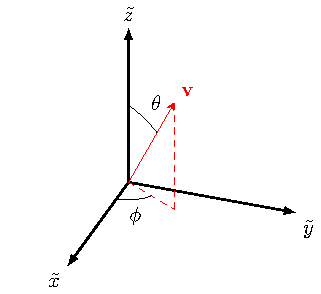
\includegraphics[width=6cm]{fig/ch13-boost.pdf}
    \caption{两参考系速度差$\boldsymbol{v}$与坐标系的关系} \label{chlg:fig_cart_sph}
\end{figure}

%我们知道,整体矢量表示$x^\mu \boldsymbol{e}_{\mu}$是Lorentz变换下的不变形式,
%即$x'^\mu \boldsymbol{e}^{\prime}_{\mu}=x^\nu \boldsymbol{e}_{\nu}$,也就是
%$\boldsymbol{e}^{\prime} X' =\boldsymbol{e} X {\color{red}\Rightarrow}
%(\boldsymbol{e}^{\prime} R^{-1})( R X') =(\boldsymbol{e} R^{-1}) (RX){\color{red}\Rightarrow}
%\tilde{\boldsymbol{e}}^{\prime} \tilde{X}' =\tilde{\boldsymbol{e}} \tilde{X}$.

关键是求解旋转矩阵$R^{-1}({\theta \phi })$的表达式.
根据我们的约定(见例题\ref{chlg:exm_GLonV}、\ref{chlg:exm_GLonB}),
旋转矩阵$R^{-1}({\theta \phi })$左作用在分量$X$上,
右作用在基矢$\boldsymbol{e}=(\boldsymbol{e}_1,\boldsymbol{e}_2,\boldsymbol{e}_3)$上.
现在考虑如图\ref{chlg:fig_cart_sph}所示的$\boldsymbol{v}$,
纯空间固有旋转$R^{-1}({\theta \phi })$相当于将$\boldsymbol{v}$(对应基矢$\boldsymbol{e}$)
旋转到$\tilde{x}$(对应基矢$\tilde{\boldsymbol{e}}$)的方向.不难求得
\begin{equation}\label{chlg:eqn_R-of-bx2b}
    R^{-1}( {\theta \phi } )  = C_{\tilde y}\left({\frac{\pi }{2} -\theta} \right) C_{\tilde z}( -\phi )
    \ \Rightarrow\  R( {\theta \phi } )  =
    {C_{\tilde  z}}(  {\phi } ) {C_{\tilde  y}} \left(  { \theta -\frac{\pi }{2}} \right) .
\end{equation}
上式计算中用到了$C_k^{-1}(\psi)=C_k(-\psi)$.则有
\begin{equation*}
    B\left( \boldsymbol{v} \right) = R{B_x}(u)R^{-1}={C_{\tilde z}}\left(  {\phi } \right)
    {C_{\tilde y}} \left(  { \theta -\frac{\pi }{2}} \right) {B_x} \left( u \right)
    {C_{\tilde y}}\left( {\frac{\pi }{2}-\theta} \right){C_{\tilde z}}\left( -\phi \right) .
\end{equation*}
经过矩阵乘法计算可以得到
\begin{small}
\begin{equation}\label{chlg:eqn_lorentz-matrix-any-v}
    B(\boldsymbol{v}) = \begin{pmatrix}
        \gamma    & -\gamma \dfrac{v_x}{c} & -\gamma \dfrac{v_y}{c} & -\gamma \dfrac{v_z}{c} \\
        -\gamma \dfrac{v_x}{c} & 1+ \dfrac{(\gamma-1)v_x^2}{v^2} &
        \dfrac{(\gamma-1)v_x v_y}{v^2} & \dfrac{(\gamma-1)v_x v_z}{v^2} \\
        -\gamma \dfrac{v_y}{c} & \dfrac{(\gamma-1)v_x v_y}{v^2} &
        1+ \dfrac{(\gamma-1)v_y^2}{v^2} & \dfrac{(\gamma-1)v_y v_z}{v^2} \\
        -\gamma \dfrac{v_z}{c} & \dfrac{(\gamma-1)v_x v_z}{v^2} &
        \dfrac{(\gamma-1)v_y v_z}{v^2} & 1+ \dfrac{(\gamma-1)v_z^2}{v^2}
    \end{pmatrix}.
\end{equation}
\end{small}
其中$\gamma^{-1}=\sqrt{1-v^2/c^2}$.
速度$\boldsymbol{v}$的分量可以由图\ref{chlg:fig_cart_sph}计算求得
\begin{equation}
    {v_x} = v\sin \theta \cos \phi, \quad
    {v_y} = v\sin \theta \sin \phi, \quad
    {v_z} = v\cos \theta  .
\end{equation}
计算中需注意$|\boldsymbol{u}|=|\boldsymbol{v}|$,即原来沿$x$轴的速度$u$的大小与任意方向速度$\boldsymbol{v}$的大小相等.
从上面伪转动矩阵可见它必然是对称的.
它穷尽了两惯性系$O$和$O'$间满足如下条件的线性变换:
\textcircled{\tiny{甲}}两坐标系相应轴是相互平行且同向;
\textcircled{\tiny{乙}}两坐标系的空间坐标原点在$t=0=t'$时重合;
\textcircled{\tiny{丙}}两坐标系速度差$\boldsymbol{v}$是常数,且方向任意.
符合这三条的Lorentz变换叫作{\heiti 伪转动}.

从物理思辨显然可得$B^{-1}(\boldsymbol{v})=B(\boldsymbol{-v})$.由于只是速度前添加负号,
所以式\eqref{chlg:eqn_lorentz-matrix-any-v}只有第一行、第一列前添加负号即可,且$00$分量
符号不变;右下角的$3\times 3$矩阵因负负得正,符号不变.

式\eqref{chlg:eqn_lorentz-matrix-any-v}作用到时空坐标,也常写成另外一种形式
\begin{equation}\label{chlg:eqn_boost-xt}
    ct'= \gamma\left( ct-\frac{\boldsymbol{v}\cdot\boldsymbol{r}}{c}\right) , \quad
    \boldsymbol{r}' = \boldsymbol{r}+(\gamma-1)\frac{\boldsymbol{v}
        \cdot\boldsymbol{r}}{v^2}\boldsymbol{v}-\gamma \frac{\boldsymbol{v}}{c} ct.
\end{equation}
其中$\boldsymbol{r}=(x,y,z)$、$\boldsymbol{v}=(v_x, v_y, v_z )$、$\boldsymbol{v}\cdot \boldsymbol{r}=v_x x+v_y y+v_z z$.

\paragraph{快度}\label{chlg:sec_rapid}
我们用{\kaishu 快度}(rapidity)来改写式\eqref{chlg:eqn_lorentz-matrix-any-v}.
我们先考虑$v_y=0=v_z$的最简单情形.
令$\tanh \theta_x=v_x/c$,就有$\gamma = \cosh \theta_x$;
则$-1<v_x/c<1$相当于$-\infty < \theta_x <+\infty$,
$\theta_x$称为{\heiti 快度};此时Lorentz矩阵可以表示为另一种形式
\begin{equation}\label{chlg:eqn_lorentz-rapid-x}
    (\Lambda_x)^{\mu}_{\cdot \nu} = 
    \begin{pmatrix}
        \cosh\theta_x  & -\sinh\theta_x & 0 & 0 \\
        -\sinh\theta_x & \cosh\theta_x  & 0 & 0 \\
        0 & 0 & 1 & 0 \\
        0 & 0 & 0 & 1 
    \end{pmatrix}.
\end{equation}

我们来看一下沿$x$轴连续进行两次Lorentz变换会是什么结果.
先进行一次Lorentz变换$\theta_2$,然后再进行第二次Lorentz变换$\theta_1$,有
\begin{equation}\label{chlg:eqn_b1b2}
    \Lambda_x(\theta_1) \Lambda_x(\theta_2) = \Lambda_x(\theta_1+\theta_2).
\end{equation}
上式以快度表示;(省略无关紧要的$y$和$z$轴)计算过程是
\begin{small}
\[\begin{pmatrix}
    \cosh\theta_1  & -\sinh\theta_1 \\
    -\sinh\theta_1 & \cosh\theta_1  
\end{pmatrix} \times
\begin{pmatrix}
    \cosh\theta_2  & -\sinh\theta_2  \\
    -\sinh\theta_2 & \cosh\theta_2   
\end{pmatrix} = 
\begin{pmatrix}
    \cosh(\theta_1+\theta_2)  & -\sinh(\theta_1+\theta_2)  \\
    -\sinh(\theta_1+\theta_2) & \cosh(\theta_1+\theta_2) 
\end{pmatrix} \]
\end{small}
上面计算利用了双曲函数和差公式
$\sinh(x \pm y) = \sinh x \cosh y \pm  \cosh x \sinh y, \ 
\cosh(x \pm y) = \cosh x \cosh y \pm  \sinh x \sinh y$.

由式\eqref{chlg:eqn_b1b2}可见用快度表示Lorentz变换时,
它是单参数子群.同理可以得到沿$y,z$方向的快度表达式:
\begin{equation*}  %\label{chlg:eqn_lorentz-rapid-yz}
    (\Lambda_y)^{\mu}_{\cdot \nu} = 
    \begin{pmatrix}
        \cosh\theta_y  & 0 & -\sinh\theta_y & 0 \\
        0 & 1  & 0 & 0 \\
        -\sinh\theta_y & 0 & \cosh\theta_y & 0 \\
        0 & 0 & 0 & 1 
    \end{pmatrix},\
    (\Lambda_z)^{\mu}_{\cdot \nu} = 
    \begin{pmatrix}
        \cosh\theta_z  & 0 & 0 & -\sinh\theta_z \\
        0 & 1  & 0 & 0 \\
        0 & 0 & 1 & 0 \\
        -\sinh\theta_z & 0 & 0 & \cosh\theta_z
    \end{pmatrix} .
\end{equation*}
当考虑$y$方向快度时,有$v_x=0=v_z$;
令$\tanh \theta_y=v_y/c$,就有$\gamma = \cosh \theta_y$;
则$-1<v_y/c<1$相当于$-\infty < \theta_y <+\infty$.
当考虑$z$方向快度时,有$v_x=0=v_y$;
令$\tanh \theta_z=v_z/c$,就有$\gamma = \cosh \theta_z$;
则$-1<v_z/c<1$相当于$-\infty < \theta_z <+\infty$.





\subsubsection{Lorentz矩阵分解}
在狭义相对论发展的初期,学者们就基本解决了Lorentz变换矩阵的分解问题;
此处的叙述参考了较新的文献\parencite{liang_zhou2009_2}附录G.9,而没有去寻找最原始的证明.

%全部三维坐标空间的固有转动群是SO(3),也就是所有\eqref{chlg:eqn_rotation}组成的集合.



\begin{proposition}\label{chlg:thm_xx-txtx}
    如果两个惯性坐标系$X$和$X'$由伪转动$B(\boldsymbol{v})$联系,并且$R\in SO(3)$,则
    $\tilde{X}\equiv RX$和$\tilde{X}'\equiv RX'$也由伪转动联系.
\end{proposition}
\begin{proof}
    设$X'=B(\boldsymbol{v})X$,并且$B(\boldsymbol{v})$是伪转动,则上节证明过程可以
    看出存在$R_0\in SO(3)$使得$B(\boldsymbol{v})=R_0B_x(u)R_0^{-1}$,因此
    $X'=R_0B_x(u)R_0^{-1}X$,从而$R_0^{-1}X'=B_x(u)R_0^{-1}X$,与$\tilde{X}\equiv RX$
    和$\tilde{X}'\equiv RX'$结合就给出$R_0^{-1}R^{-1}\tilde{X}'=B_x(u)R_0^{-1}R^{-1}\tilde{X}$.
    令$R_1 = RR_0$,则$\tilde{X}'=R_{1}B_x(u)R_1^{-1}\tilde{X}$.
    因此$\tilde{X}$和$\tilde{X}'$也由伪转动联系.
\end{proof}

\begin{proposition}\label{chlg:thm_b-rbr}
    对于任意伪转动$B(\boldsymbol{v})$,以及任意$R\in SO(3)$,都有
        $B(R\boldsymbol{v}) = R B(\boldsymbol{v}) R^{-1}$.
    此式左边$R\boldsymbol{v}$的分量是$(R\boldsymbol{v})^i = R^i_{\cdot j}v^j$,是三维空间矢量.
    右边的$R$是四维时空的转动,两者有一一对应关系\eqref{chlg:eqn_rotation-4d}.
\end{proposition}
\begin{proof}
    设有两个惯性参考系$O$和$O'$,在它们中分别建立直角坐标系$O-xyz$和$O'-x'y'z'$;
    这两个坐标系符合上一节末尾给出的伪转动定义中的三个条件;$O'$系相对于$O$系以
    常速度$\boldsymbol{v}$运动,$\boldsymbol{v}$在$O$系的分量是$\boldsymbol{v}=v^i \boldsymbol{e}_i$.
    由于$O$和$O'$都是惯性系,那就存在联系两个坐标系的伪转动$B(\boldsymbol{v})$,其表达式
    是\eqref{chlg:eqn_lorentz-matrix-any-v},即$X' = {B}( \boldsymbol{v} )X$.
    
    设$R$是纯空间固有转动,再令
    $\tilde{X}=RX$,$\tilde{X}'=RX'$;显然$\tilde{X}$和$\tilde{X}'$都是惯性坐标系,
    那么由命题\ref{chlg:thm_xx-txtx}可知$\tilde{X}$和$\tilde{X}'$也由某个伪转动联系着.
    两个惯性系参考系$\tilde{X}$和$\tilde{X}'$的速度差仍旧是$\boldsymbol{v}$,只不过$\boldsymbol{v}$在
    $\tilde{X}$坐标系中的分量变成了$\boldsymbol{v}=\tilde{v}^i { \tilde{\boldsymbol{e}}}_i=
    {v}^i { {\boldsymbol{e}}}_i$,其中
    $\tilde{\boldsymbol{e}}_i = \boldsymbol{e}_j R^j_{\cdot i}$,$\tilde{v}^i =  R^i_{\cdot k}v^k$.
    纯空间转动不改变$\boldsymbol{v}$的大小,只改变它的分量值.
    联系两个坐标系$\tilde{X}$和$\tilde{X}'$的伪转动是$B(\tilde{\boldsymbol{v}})$,其表达式
    仍旧是\eqref{chlg:eqn_lorentz-matrix-any-v},只不过,速度的分量变成了$\tilde{\boldsymbol{v}}$
    的分量.读者需注意式\eqref{chlg:eqn_lorentz-matrix-any-v}的具体表达式是和速度的分量相关的.
    因此有$\tilde{X}'=B(\tilde{\boldsymbol{v}})\tilde{X}=B( R^i_{\cdot j}v^j)\tilde{X}$.
    再与式$ \tilde X' = RX' = R{B}\left( \boldsymbol{v} \right)X
    =  \left[ {R{B}\left( \boldsymbol{v} \right){R^{ - 1}}} \right]\tilde X $相比较,
    可知定理得证.
\end{proof}



\begin{theorem} \label{chlg:thm_lorentz-decompose-r}
    对于任意的$ \Lambda \in L^{\uparrow}_{+}$,
    存在唯一的伪转动$B(\boldsymbol{v})$以及唯一的纯空间固有转动$R$,
    使得$\Lambda = B(\boldsymbol{v}) R = R'B(\boldsymbol{v})$,具体表达式见证明过程.
\end{theorem}
\begin{proof}
    \fbox{甲}若$\Lambda$是伪转动,则只需取$B(\boldsymbol{v})=\Lambda,R=I$即可.
    唯一性见\fbox{丙}.
    
    \fbox{乙}下面证明$\Lambda$不是伪转动情形.
    已知伪转动$B(\boldsymbol{v})$是对称的,纯空间转动$R$形式是\eqref{chlg:eqn_rotation-4d}.
    把$B(\boldsymbol{v})$和$R$分别记成
    \begin{equation}
        B(\boldsymbol{v}) = \begin{pmatrix}
            B^0_{\cdot 0}  & B^0_{\cdot 1} & B^0_{\cdot 2} & B^0_{\cdot 3} \\
            B^1_{\cdot 0}  & B^1_{\cdot 1} & B^1_{\cdot 2} & B^1_{\cdot 3} \\
            B^2_{\cdot 0}  & B^2_{\cdot 1} & B^2_{\cdot 2} & B^2_{\cdot 3} \\
            B^3_{\cdot 0}  & B^3_{\cdot 1} & B^3_{\cdot 2} & B^3_{\cdot 3}
        \end{pmatrix}, \qquad
        R = \begin{pmatrix}
            1    & 0 & 0 & 0 \\
            0 & R^1_{\cdot 1} & R^1_{\cdot 2} & R^1_{\cdot 3} \\
            0 & R^2_{\cdot 1} & R^2_{\cdot 2} & R^2_{\cdot 3} \\
            0 & R^3_{\cdot 1} & R^3_{\cdot 2} & R^3_{\cdot 3}
        \end{pmatrix}.
    \end{equation}
    那么$B(\boldsymbol{v})$和$R$相乘的第一列是
    \begin{equation}\label{chlg:eqn_ld-tmp1}
        B(\boldsymbol{v})R=\begin{pmatrix}
            B^0_{\cdot 0} & \cdots & \cdots& \cdots\\
            B^1_{\cdot 0} & \cdots & \cdots& \cdots\\
            B^2_{\cdot 0} & \cdots & \cdots& \cdots\\
            B^3_{\cdot 0} & \cdots & \cdots& \cdots
        \end{pmatrix},\ \text{而}\
        \Lambda=\begin{pmatrix}
            \Lambda^0_{\cdot 0} & \Lambda^0_{\cdot 1} & \Lambda^0_{\cdot 2}& \Lambda^0_{\cdot 3}\\
            \Lambda^1_{\cdot 0} & \cdots & \cdots& \cdots\\
            \Lambda^2_{\cdot 0} & \cdots & \cdots& \cdots\\
            \Lambda^3_{\cdot 0} & \cdots & \cdots& \cdots
        \end{pmatrix} .
    \end{equation}
    本定理中要证明$\Lambda=B(\boldsymbol{v})R$,根据式\eqref{chlg:eqn_lorentz-matrix-any-v}以
    及上式可以令
    \begin{equation}
        B^{0}_{\cdot 0}(\boldsymbol{v})=\gamma = \Lambda^0_{\cdot 0}, \quad
        B^{i}_{\cdot 0}(\boldsymbol{v})=-\gamma\frac{v^i}{c}= {\Lambda^i_{\cdot 0}}, \ \text{即}\
        {v^i}= - {c}\frac{\Lambda^i_{\cdot 0}}{\Lambda^0_{\cdot 0}}.
    \end{equation}
    号差$+2$的Lorentz度规并不改变$v$纯空间分量正负号,故$v_i=v^i$($i=1,2,3$).
    利用\eqref{chlg:eqn_ltm00}可以证明$|v|<c$:
    \begin{equation*}
        \sum_{i=1}^{3}\left( \frac{v^i}{c}\right)^2
        =\sum_{i=1}^{3}\left( \frac{\Lambda^i_{\cdot 0}}{\Lambda^0_{\cdot 0}}\right)^2
        =\frac{1}{(\Lambda^0_{\cdot 0})^2} \sum_{i=1}^{3}\left( {\Lambda^i_{\cdot 0}}\right)^2
        =\frac{1}{1+\sum_{j}\left( {\Lambda^j_{\cdot 0}}\right)^2}
        \sum_{i=1}^{3}\left( {\Lambda^i_{\cdot 0}}\right)^2    <1  .
    \end{equation*}
    即上面定义的速度是亚光速的.
    先求出速度$\boldsymbol{v}$的大小(要参考\eqref{chlg:eqn_ltm00}).
    \setlength{\mathindent}{0em}
    \begin{equation}\label{chlg:eqn_ltdbr-v}
        v^2 = \sum_{i=1}^{3}v_i^2 =  \dfrac{c^2}{(\Lambda^0_{\cdot 0})^2} \sum_{i=1}^{3}
        ({\Lambda^i_{\cdot 0}})^2
        = \dfrac{c^2}{(\Lambda^0_{\cdot 0})^2}\left(  (\Lambda^0_{\cdot 0})^2 -1\right)
        = \dfrac{c^2}{\gamma^2}\left(  \gamma^2 -1\right).
    \end{equation}\setlength{\mathindent}{2em}
    有了速度分量,
    根据式\eqref{chlg:eqn_lorentz-matrix-any-v}就可以构造出一伪转动$B(\boldsymbol{v})$:
    \begin{equation}\label{chlg:eqn_ltdbr-b}
        \begin{aligned}
            B^{0}_{\cdot 0}(\boldsymbol{v}) &= B^{0}_{\cdot 0}(-\boldsymbol{v}) =  \Lambda ^{0}_{\cdot 0}, \qquad
            B^{i}_{\cdot 0}(\pm\boldsymbol{v}) = \pm \Lambda ^{i}_{\cdot 0}, \\
            B^{i}_{\cdot j}(\boldsymbol{v}) &= B^{i}_{\cdot j}(-\boldsymbol{v}) =
            \delta^i_j + (\gamma-1)\dfrac{v_i v_j}{v^2} =
            \delta^i_j + \dfrac{\Lambda ^{i}_{\cdot 0}\Lambda ^{{\color{red}j}}_{\cdot 0}}
            {1 + \Lambda ^{0}_{\cdot 0} } .
        \end{aligned}
    \end{equation}
    需要注意$B^{i}_{\cdot j}$值右端$\Lambda ^{j}_{\cdot 0}$中的$j$是上标.
    我们已经构造出一个伪转动\eqref{chlg:eqn_ltdbr-b},
    由于我们要证明$\Lambda=B(\boldsymbol{v})R$,只需令$R =B^{-1}(\boldsymbol{v})\Lambda=B(-\boldsymbol{v})\Lambda $,
    把式\eqref{chlg:eqn_ltdbr-b}带入此式就可以得到
    \begin{equation}\label{chlg:eqn_ltdbr-r}
        R^{0}_{\cdot 0} = 1, \quad    R^{i}_{\cdot 0} = R^{0}_{\cdot i} = 0, \quad
        R^{i}_{\cdot j} = \Lambda^i_{\cdot j} - \dfrac{\Lambda ^{i}_{\cdot 0}
            \Lambda ^{0}_{\cdot j}}{1 + \Lambda ^{0}_{\cdot 0} }.
    \end{equation}
    可以验证这个矩阵是正交矩阵,可见$R\in SO(3)$.
    \uwave{\kaishu 这步验证十分重要,必不可少}.
    验证过程中的矩阵乘法会用到式
    \eqref{chlg:eqn_ltm00},\eqref{chlg:eqn_ltm0i}和\eqref{chlg:eqn_ltmik}.
    
    现在回顾一下证明的大体过程,按照一定规则先构造出伪转动\eqref{chlg:eqn_ltdbr-b},然后求出了一个
    矩阵\eqref{chlg:eqn_ltdbr-r},在验证了\eqref{chlg:eqn_ltdbr-r}是正交矩阵后,
    就证明了任意Lorentz矩阵$\Lambda$都可进行分解$\Lambda=B(\boldsymbol{v})R$,分解后的$B(\boldsymbol{v})$与$R$表达式见上.
    
    \fbox{丙}下面证明分解的唯一性.设$\Lambda$另有分解$\Lambda={B}(\boldsymbol{u})\tilde{R}$,则有
    ${B}(\boldsymbol{u})\tilde{R}=B(\boldsymbol{v})R$,由此容易得到
    ${B}(\boldsymbol{u})=B(\boldsymbol{v})R\tilde{R}^{-1}$,而$R\tilde{R}^{-1}$依旧是纯空间转动.
    由式\eqref{chlg:eqn_ld-tmp1}易得
    ${B}^{0}_{\cdot 0}(\boldsymbol{u})= \Lambda^0_{\cdot 0}=B^{0}_{\cdot 0}(\boldsymbol{v})$,
    ${B}^{i}_{\cdot 0}(\boldsymbol{u})= {\Lambda^i_{\cdot 0}} =B^{i}_{\cdot 0}(\boldsymbol{v})$.
    这说明$\gamma_u =\gamma_v$,$\gamma_u u^i=\gamma_v v^i{\  \Rightarrow \  } u^i=v^i$,
    也就是${B}(\boldsymbol{u}) \equiv B(\boldsymbol{v})$,    从而$\tilde{R}\equiv R$.
    
    
    $\Lambda = R'B(\boldsymbol{v})$的分解证明留给读者当练习.
\end{proof}

%\subsubsection{一般Lorentz变换}
%本小节主要讨论时空$1+3$分解后的一般Lorentz变换.
%式\eqref{chlg:eqn_boost-xt}给出了初始时刻相应坐标轴相互平行、同向的情形;
%下面讨论坐标轴不相互平行的情形.根据定理\ref{chlg:thm_lorentz-decompose-r}可知:
%这种Lorentz变换还相差一个纯空间转动.
%我们用$D$表示这个转动,则有
%\begin{equation}\label{chlg:eqn_lorentz-xt}
%    t'= \gamma_v \left( t-\frac{\boldsymbol{v}\cdot\boldsymbol{r}}{c^2}\right) , \qquad
%    \boldsymbol{r}' = D\boldsymbol{r}+D\boldsymbol{v} 
%    \left((\gamma_v-1)\frac{\boldsymbol{v}\cdot\boldsymbol{r}}{v^2}-\gamma_v t \right).
%\end{equation}
%这就是说$\boldsymbol{r}_{\parallel}\equiv D \boldsymbol{r}$所处坐标系与$\boldsymbol{r}'$所处坐标系的坐标轴相互平行、同向.
%式\eqref{chlg:eqn_lorentz-xt}中第二式中圆括号内是标量,
%即$(\gamma_v-1)\frac{\boldsymbol{v}\cdot\boldsymbol{r}}{v^2}-\gamma_v t $是标量;
%它的数值不随纯空间转动$D$而改变.$D$只改变$\boldsymbol{r}$、$\boldsymbol{v}$的方向,不改变其大小;
%对$\boldsymbol{v}$的转动($D$)操作正好是$O'$系测量$O$系的速度$\boldsymbol{v}'$的负值,即
%\begin{equation}\label{chlg:eqn_vDvp}
%    D \boldsymbol{v} = - \boldsymbol{v}' .
%\end{equation}
%
%对式\eqref{chlg:eqn_lorentz-xt}取微分,注意$D$、$\boldsymbol{v}$、$\gamma_v$都是常数,
%微分只对$t$、$t'$、$\boldsymbol{r}$、$\boldsymbol{r}'$起作用.
%取完微分后,求商即可得到速度($\boldsymbol{u}={\rm d}\boldsymbol{r}/{\rm d}t,\, 
%\boldsymbol{u}'={\rm d}\boldsymbol{r}'/{\rm d}t' $)变换公式
%\begin{equation}\label{chlg:eqn_u2up}
%    \boldsymbol{u}' = \frac{1}{1-\boldsymbol{v}\cdot \boldsymbol{u}/c^2}\left(
%    \gamma_v^{-1} D \boldsymbol{u} + \frac{\gamma_v-1}{\gamma_v}
%    \frac{\boldsymbol{u}\cdot \boldsymbol{v}}{v^2} D\boldsymbol{v}-D\boldsymbol{v} \right) .
%\end{equation}
%
%%\begin{equation}
%%    (\gamma_v^2 v^2/c^2)= \frac{1}{1-\frac{v^2}{c^2}} v^2/c^2
%%    =\gamma_v^2-1=(\gamma_v+1)(\gamma_v-1) .
%%\end{equation}
%
%
%下面列出一个常用公式:
%\begin{equation}\label{chlg:eqn_ggg}
%    \gamma_{u'}= \gamma_v \gamma_u\left(1-\frac{\boldsymbol{v}\cdot \boldsymbol{u}}{c^2}\right) 
%    \quad \text{和} \quad
%    \gamma_{u}= \gamma_v \gamma_{u'}\left(1+\frac{\boldsymbol{v}\cdot \boldsymbol{u}'}{c^2}\right) .
%\end{equation}
%只需将各种速度带入相应Lorentz因子,然后直接计算即可证明.
%
%%证明过程如下:
%%上式等价于证明
%%\begin{equation}\label{chlg:eqn_tmpggg}
%%    \left(1- \frac{v^2}{c^2} \right)\left(1- \frac{u^2}{c^2} \right)
%%    =\left(1-\frac{\boldsymbol{v}\cdot \boldsymbol{u}}{c^2}\right)^2
%%    \left(1- \frac{u^{\prime 2}}{c^2} \right) .
%%\end{equation}
%%下式推导中注意利用$D$是正交矩阵.
%%\begin{align*}
%%    &\gamma_v^{2}(1-\boldsymbol{v}\cdot \boldsymbol{u}/c^2)^2 \boldsymbol{u}'\cdot \boldsymbol{u}' =\left[
%%    D \boldsymbol{u} + \left((\gamma_v-1)
%%    \frac{\boldsymbol{u}\cdot \boldsymbol{v}}{v^2}-\gamma_v\right) D\boldsymbol{v} \right]^2 \\
%%    =& D \boldsymbol{u}\cdot D \boldsymbol{u}  + 2 D \boldsymbol{u} \cdot
%%    \left((\gamma_v-1)\frac{\boldsymbol{u}\cdot \boldsymbol{v}}{v^2}-\gamma_v\right) D\boldsymbol{v} 
%%    + \left((\gamma_v-1)\frac{\boldsymbol{u}\cdot \boldsymbol{v}}{v^2}-\gamma_v\right)^2 D\boldsymbol{v} \cdot D\boldsymbol{v}  \\
%%    =& u^2  + 2 
%%    \left((\gamma_v-1)\frac{\boldsymbol{u}\cdot \boldsymbol{v}}{v^2}-\gamma_v\right) \boldsymbol{u} \cdot\boldsymbol{v} 
%%    + \left((\gamma_v-1)\frac{\boldsymbol{u}\cdot \boldsymbol{v}}{v^2}-\gamma_v\right)^2 v^2  
%%\end{align*}
%%我们可以来证明式\eqref{chlg:eqn_tmpggg}了.
%%\begin{align*}
%%    &\left(1-\frac{\boldsymbol{v}\cdot \boldsymbol{u}}{c^2}\right)^2
%%    \left(1- \frac{u^{\prime 2}}{c^2} \right)
%%    =\left(1-\frac{\boldsymbol{v}\cdot \boldsymbol{u}}{c^2}\right)^2
%%    -\left(1-\frac{\boldsymbol{v}\cdot \boldsymbol{u}}{c^2}\right)^2 \frac{u^{\prime 2}}{c^2} \\
%%    =&\left(1-\frac{\boldsymbol{v}\cdot \boldsymbol{u}}{c^2}\right)^2-
%%    \gamma_v^{-2} c^{-2} \left[u^2  + 2 
%%    \left((\gamma_v-1)\frac{\boldsymbol{u}\cdot \boldsymbol{v}}{v^2}-\gamma_v\right) \boldsymbol{u} \cdot\boldsymbol{v} 
%%    + \left((\gamma_v-1)\frac{\boldsymbol{u}\cdot \boldsymbol{v}}{v^2}-\gamma_v\right)^2 v^2  \right] \\
%%    =&1 + \frac{(\boldsymbol{v}\cdot \boldsymbol{u})^2}{c^4} - 2\frac{\boldsymbol{v}\cdot \boldsymbol{u}}{c^2}
%%    -\gamma_v^{-2} c^{-2} u^2  \\
%%    &- 2 \gamma_v^{-2} c^{-2}
%%    \left((\gamma_v-1)\frac{\boldsymbol{u}\cdot \boldsymbol{v}}{v^2}-\gamma_v\right) \boldsymbol{u} \cdot\boldsymbol{v} \\
%%    &- \gamma_v^{-2} c^{-2}\left((\gamma_v-1)\frac{\boldsymbol{u}\cdot \boldsymbol{v}}{v^2}-\gamma_v\right)^2 v^2   \\
%%    =&1 + \frac{(\boldsymbol{v}\cdot \boldsymbol{u})^2}{c^4} - 2\frac{\boldsymbol{v}\cdot \boldsymbol{u}}{c^2}
%%    -\gamma_v^{-2} \frac{u^2}{c^2}   \\
%%    &- 2 \gamma_v^{-2} (\gamma_v-1)\frac{\boldsymbol{u}\cdot \boldsymbol{v}}{v^2} \frac{\boldsymbol{u}\cdot \boldsymbol{v}}{c^2} 
%%    + 2 \gamma_v^{-1}  \frac{\boldsymbol{u}\cdot \boldsymbol{v}}{c^2}\\
%%    &- \left[\left(\frac{\gamma_v-1}{\gamma_v}\frac{\boldsymbol{u}\cdot \boldsymbol{v}}{v^2} \right)^2 
%%    -2\frac{\gamma_v-1}{\gamma_v}\frac{\boldsymbol{u}\cdot \boldsymbol{v}}{v^2}    +1\right]\frac{v^2}{c^2}   \\
%%    =&1   -\gamma_v^{-2} \frac{u^2}{c^2}    -\frac{v^2}{c^2}   \\
%%    &+ \frac{(\boldsymbol{v}\cdot \boldsymbol{u})^2}{c^4 }
%%    - 2 \gamma_v^{-2} (\gamma_v-1)\frac{\boldsymbol{u}\cdot \boldsymbol{v}}{v^2} \frac{\boldsymbol{u}\cdot \boldsymbol{v}}{c^2}
%%    - \left(\frac{\gamma_v-1}{\gamma_v}\frac{\boldsymbol{u}\cdot \boldsymbol{v}}{v^2} \right)^2 \frac{v^2}{c^2}  \\
%%    &+ 2 \gamma_v^{-1}  \frac{\boldsymbol{u}\cdot \boldsymbol{v}}{c^2}
%%    +2\frac{\gamma_v-1}{\gamma_v}\frac{\boldsymbol{u}\cdot \boldsymbol{v}}{v^2} \frac{v^2}{c^2} 
%%    - 2\frac{\boldsymbol{v}\cdot \boldsymbol{u}}{c^2} .
%%\end{align*}
%%上式最后一步中$\boldsymbol{v}\cdot \boldsymbol{u}$前的系数之和正好为零,故有
%%\begin{align}
%%    \left(1-\frac{\boldsymbol{v}\cdot \boldsymbol{u}}{c^2}\right)^2
%%    \left(1- \frac{u^{\prime 2}}{c^2} \right)
%%    =1   -\gamma_v^{-2} \frac{u^2}{c^2}    -\frac{v^2}{c^2}
%%    =\left(1- \frac{v^2}{c^2} \right)\left(1- \frac{u^2}{c^2} \right).
%%\end{align}
%
%
%%逆变换的证明过程如下:
%%上式等价于证明
%%\begin{equation}\label{chlg:eqn_tmpggg}
%%    \left(1- \frac{v^2}{c^2} \right)\left(1- \frac{u'^2}{c^2} \right)
%%    =\left(1+\frac{\boldsymbol{v}\cdot \boldsymbol{u}'}{c^2}\right)^2
%%    \left(1- \frac{w^2}{c^2} \right) .
%%\end{equation}
%%下式推导中注意利用$D$是正交矩阵以及速度逆变换公式\eqref{chsr:eqn_boost-u-inv}.
%%\begin{align*}
%%    &\gamma_v^{2}(1+\boldsymbol{v}\cdot \boldsymbol{u}'/c^2)^2 \boldsymbol{w}\cdot \boldsymbol{w} =\left[
%%    D \boldsymbol{u}' + \left((\gamma_v-1)
%%    \frac{\boldsymbol{u}'\cdot \boldsymbol{v}}{v^2}+\gamma_v\right) D\boldsymbol{v} \right]^2 \\
%%    =& D \boldsymbol{u}'\cdot D \boldsymbol{u}'  + 2 D \boldsymbol{u}' \cdot
%%    \left((\gamma_v-1)\frac{\boldsymbol{u}'\cdot \boldsymbol{v}}{v^2}+\gamma_v\right) D\boldsymbol{v} 
%%    + \left((\gamma_v-1)\frac{\boldsymbol{u}'\cdot \boldsymbol{v}}{v^2}+\gamma_v\right)^2 D\boldsymbol{v} \cdot D\boldsymbol{v}  \\
%%    =& u'^2  + 2 
%%    \left((\gamma_v-1)\frac{\boldsymbol{u}'\cdot \boldsymbol{v}}{v^2}+\gamma_v\right) \boldsymbol{u}' \cdot\boldsymbol{v} 
%%    + \left((\gamma_v-1)\frac{\boldsymbol{u}'\cdot \boldsymbol{v}}{v^2}+\gamma_v\right)^2 v^2  
%%\end{align*}
%%我们可以来证明式\eqref{chlg:eqn_tmpggg}了.
%%\begin{align*}
%%    &\left(1+\frac{\boldsymbol{v}\cdot \boldsymbol{u}'}{c^2}\right)^2
%%    \left(1- \frac{w^2}{c^2} \right)
%%    =\left(1+\frac{\boldsymbol{v}\cdot \boldsymbol{u}'}{c^2}\right)^2
%%    -\left(1+\frac{\boldsymbol{v}\cdot \boldsymbol{u}'}{c^2}\right)^2 \frac{w^2}{c^2} \\
%%    =&\left(1+\frac{\boldsymbol{v}\cdot \boldsymbol{u}'}{c^2}\right)^2
%%    -\gamma_v^{-2} c^{-2} \left[u'^2  + 2 
%%    \left((\gamma_v-1)\frac{\boldsymbol{u}'\cdot \boldsymbol{v}}{v^2}+\gamma_v\right) \boldsymbol{u}' \cdot\boldsymbol{v} 
%%    + \left((\gamma_v-1)\frac{\boldsymbol{u}'\cdot \boldsymbol{v}}{v^2}+\gamma_v\right)^2 v^2 \right] \\
%%    =& 1 + 2 \frac{\boldsymbol{v}\cdot \boldsymbol{u}'}{c^2} + \frac{(\boldsymbol{v}\cdot \boldsymbol{u}')^2}{c^4} -\gamma_v^{-2} c^{-2} u'^2 
%%    -\gamma_v^{-2} c^{-2} 2\left((\gamma_v-1)\frac{\boldsymbol{u}'\cdot \boldsymbol{v}}{v^2}+\gamma_v\right) \boldsymbol{u}' \cdot\boldsymbol{v} 
%%    -\gamma_v^{-2} c^{-2} \left((\gamma_v-1)\frac{\boldsymbol{u}'\cdot \boldsymbol{v}}{v^2}+\gamma_v\right)^2 v^2 \\
%%    =&1 + 2 \frac{\boldsymbol{v}\cdot \boldsymbol{u}'}{c^2} + \frac{(\boldsymbol{v}\cdot \boldsymbol{u}')^2}{c^4} -\gamma_v^{-2} c^{-2} u'^2 
%%    -2 \frac{\gamma_v-1}{\gamma_v^{2}}\frac{(\boldsymbol{u}'\cdot \boldsymbol{v})^2}{c^2 v^2}
%%    -\frac{2}{\gamma_v}\frac{\boldsymbol{u}' \cdot\boldsymbol{v}}{c^2}  \\
%%    &- \left[\left(\frac{\gamma_v-1}{\gamma_v}\right)^2\frac{(\boldsymbol{u}'\cdot \boldsymbol{v})^2}{v^4}
%%    +2\frac{\gamma_v-1}{\gamma_v}\frac{\boldsymbol{u}'\cdot \boldsymbol{v}}{v^2}    +1\right] \frac{v^2}{c^2} \\
%%    =&1 -\gamma_v^{-2} c^{-2} u'^2 - \frac{v^2}{c^2} \\
%%    & + 2 \frac{\boldsymbol{v}\cdot \boldsymbol{u}'}{c^2} -\frac{2}{\gamma_v}\frac{\boldsymbol{u}' \cdot\boldsymbol{v}}{c^2}
%%    - 2\frac{\gamma_v-1}{\gamma_v}\frac{\boldsymbol{u}'\cdot \boldsymbol{v}}{v^2} \frac{v^2}{c^2} \\
%%    & + \frac{(\boldsymbol{v}\cdot \boldsymbol{u}')^2}{c^4} -2 \frac{\gamma_v-1}{\gamma_v^{2}}\frac{(\boldsymbol{u}'\cdot \boldsymbol{v})^2}{c^2 v^2}
%%    -\left(\frac{\gamma_v-1}{\gamma_v}\right)^2\frac{(\boldsymbol{u}'\cdot \boldsymbol{v})^2}{v^4}\frac{v^2}{c^2}
%%\end{align*}
%%上式最后一步中$\boldsymbol{v}\cdot \boldsymbol{u}$前的系数之和正好为零,故有
%%\begin{align}
%%    \left(1+\frac{\boldsymbol{v}\cdot \boldsymbol{u}'}{c^2}\right)^2
%%    \left(1- \frac{w^2}{c^2} \right)
%%    =1   -\gamma_v^{-2} \frac{u'^2}{c^2}    -\frac{v^2}{c^2}
%%    =\left(1- \frac{v^2}{c^2} \right)\left(1- \frac{u'^2}{c^2} \right).
%%\end{align}











\index[physwords]{Lorentz代数}  \index[physwords]{Lorentz代数}

\subsubsection{Lorentz代数}
正时固有Lorentz群$SO^{+}(1,3)$有六个实参数来描述,其中固有转动占三个,伪转动占三个.
我们通过单参数子群来求取其李代数.
在\S\ref{chlar:sec_LA-su2so3}中,我们
找到了$SO(3)$群的三个单参数子群;只需将其拓展到四维空间即可.
它们是
\begin{small}
\begin{equation}\label{chlg:eqn_LA-so13-r}
    r_1=\begin{pmatrix}
        0&0&0&0\\
        0&0 & 0 & 0 \\
        0&0& 0 & -1 \\
        0&0 & 1 & 0
    \end{pmatrix},\ 
    r_2=\begin{pmatrix}
        0&0&0&0\\
        0&0 & 0 & 1 \\
        0&0 & 0 & 0 \\
        0&-1 & 0 & 0
    \end{pmatrix},\ 
    r_3=\begin{pmatrix}
        0&0&0&0\\
        0&0 & - 1 & 0 \\
        0&1& 0 & 0 \\
        0&0 & 0 & 0
    \end{pmatrix} .
\end{equation}
\end{small}

第\pageref{chlg:sec_rapid}页中,由快度描述的伪转动也是单参数子群.
只需对式\eqref{chlg:eqn_lorentz-rapid-x}中所有矩阵元求$\theta_x$的导数,并在$\theta_x=0$取值,即
\begin{equation}
    b_1=\left.\frac{{\rm d}\Lambda_x(\theta_x)}{{\rm d}\theta_x}\right|_{\theta_x=0} \quad
    b_2=\left.\frac{{\rm d}\Lambda_y(\theta_y)}{{\rm d}\theta_y}\right|_{\theta_y=0} \quad
    b_3=\left.\frac{{\rm d}\Lambda_z(\theta_z)}{{\rm d}\theta_z}\right|_{\theta_z=0} .
\end{equation}
由上式计算出结果,得
\begin{small}
\setlength{\mathindent}{0em}
\begin{equation}\label{chlg:eqn_LA-so13-b}
    b_1=  \begin{pmatrix}
        0  & -1 & 0 & 0 \\
        -1 & 0  & 0 & 0 \\
        0 & 0 & 0 & 0 \\
        0 & 0 & 0 & 0 
    \end{pmatrix},\ 
    b_2 =  \begin{pmatrix}
        0  & 0 & -1 & 0 \\
        0 & 0  & 0 & 0 \\
        -1 & 0 & 0 & 0 \\
        0 & 0 & 0 & 0 
    \end{pmatrix},\ 
    b_3 =  \begin{pmatrix}
        0  & 0 & 0 & -1 \\
        0 & 0  & 0 & 0 \\
        0 & 0 & 0 & 0 \\
        -1 & 0 & 0 & 0 
    \end{pmatrix} .
\end{equation} \setlength{\mathindent}{2em}
\end{small}

通过直接计算,可以得到这些矩阵的对易关系(李积)如下
\begin{equation}\label{chlg:eqn_LA-so13-comm}
    [r_i, r_j] = \sum_k \epsilon_{ijk} r_k,\quad
    [b_i, r_j] = \sum_k \epsilon_{ijk} b_k,\quad
    [b_i, b_j] = -\sum_k \epsilon_{ijk} r_k.
\end{equation}
其中$i,j,k=1,2,3$;$\epsilon_{ijk}=\delta^{123}_{ijk}$,定义见式\eqref{chmla:eqn_gkd}.
式\eqref{chlg:eqn_LA-so13-r}、\eqref{chlg:eqn_LA-so13-b}连同
对易关系\eqref{chlg:eqn_LA-so13-comm}构成了$\mathfrak{so}^{+}(1,3)$李代数.


%\begin{example}
%    结构常数、Killing型、Casimir算子.
%\end{example}


物理学上较喜欢用厄米或反厄米矩阵来表示生成元,即作如下变换
\begin{equation}\label{chlg:eqn_LA-so13-JK}
    J_i = \mathbbm{i} r_i,\qquad  K_i = \mathbbm{i} b_i .
\end{equation}
那么对易关系\eqref{chlg:eqn_LA-so13-comm}变成(省略了求和符号):
\begin{equation}\label{chlg:eqn_LA-so13-comm-JK}
    [J_i, J_j] = \mathbbm{i} \epsilon_{ijk} J_k,\quad
    [J_i, K_j] = \mathbbm{i} \epsilon_{ijk} K_k,\quad
    [K_i, K_j] = -\mathbbm{i}\epsilon_{ijk} J_k.
\end{equation}
厄米矩阵$J$、反厄米矩阵$K$(即式\eqref{chlg:eqn_LA-so13-JK})及其
对易关系\eqref{chlg:eqn_LA-so13-comm-JK}是$\mathfrak{so}^{+}(1,3)$李代数
的另外一种常用表示.


%反之,我们也可以从无穷小形式$\omega_{\rho\sigma}$出发,通过指数映射得到
%一般形式的Lorentz变换$\Lambda^\mu_{\hphantom{\mu}\rho}$.由下式出发
%\begin{align*}
%    \omega^\mu_{\hphantom{\mu}\nu} =& \eta^{\mu\rho} \omega_{\rho\nu}
%    =\frac{1}{2}( \eta^{\mu\rho} \omega_{\rho\nu} - \eta^{\mu\rho} \omega_{\nu\rho})
%    =\frac{1}{2}( \eta^{\mu\rho} \delta^\sigma_\nu - \eta^{\mu\sigma} \delta^\rho_\nu ) \omega_{\rho\sigma}.
%\end{align*}
若我们定义($\eta={\rm diag}(-1,1,1,1)$)
\begin{equation}\label{chlg:eqn_LJw}
    (\mathcal{J}^{\rho\sigma})^\mu_{\hphantom{\mu}\nu} \equiv 
    \mathbbm{i} ( \eta^{\mu\sigma} \delta^\rho_\nu -\eta^{\mu\rho} \delta^\sigma_\nu).
\end{equation}
上式为Lorentz代数的整体形式.则有
\begin{align}
    \{\mathcal{J}^{10},\mathcal{J}^{20},\mathcal{J}^{30} \} =\{K_1,K_2,K_3\}, \
    \{\mathcal{J}^{23},\mathcal{J}^{31},\mathcal{J}^{12} \} =\{J_1,J_2,J_3\}.
\end{align}
那么一般Lorentz变换可表示为
\begin{equation}
    \Lambda^\mu_{\hphantom{\mu}\nu} = \exp\left( -\frac{\mathbbm{i}}{2}\omega_{\rho\sigma}
    (\mathcal{J}^{\rho\sigma})^\mu_{\hphantom{\mu}\nu} \right) .
\end{equation}
通过矩阵的指数运算可以得到$\exp(-\mathbbm{i} \alpha J_1)= C_x(\alpha)$
(见式\eqref{chlg:eqn_rotation-x});与之类似,$J_2,J_3$的矩阵指数
为式\eqref{chlg:eqn_rotation-zy}.
同样,$\exp(-\mathbbm{i} \theta K_1)= \Lambda_x(\theta)$,
即式\eqref{chlg:eqn_lorentz-rapid-x};另外两个的矩阵指数
($\exp(-\mathbbm{i} \theta K_2)$、$\exp(-\mathbbm{i} \theta K_3)$)
自然是$y$、$z$方向的伪转动.
这些计算略显繁琐,但没有难度;也可借助计算机符号软件完成.


在\S\ref{chlar:sec_LA-su2so3}中,我们建立了$\mathfrak{so}(3)$李代数矩阵基矢量和微分基矢量间的同构关系;
仿照那里的做法,可以建立Lorentz李代数$\mathfrak{so}^{+}(1,3)$矩阵基矢量和微分基矢量间的同构关系$\Psi$.
\begin{small}
\setlength{\mathindent}{0em}
\begin{equation}\label{chlg:eqn_LA-so13-JK-diff}
    \hat{J}_i=\Psi(J_i)= -\frac{\mathbbm{i}}{2}\epsilon_{ijk} \left(x^j\frac{\partial }{\partial x^k}
    - x^k\frac{\partial }{\partial x^j}\right), \ 
    \hat{K}_i=\Psi(K_i)= \mathbbm{i} \left(t\frac{\partial }{\partial x^i}+  x^i\frac{\partial }{\partial t}\right) .
\end{equation} \setlength{\mathindent}{2em}
\end{small}
因$x^0 = t=-x_0$,故$\Psi(K_i)$中圆括号内两部分符号相同.
通过直接计算可以验证微分形式的基矢量对易关系与\eqref{chlg:eqn_LA-so13-comm-JK}式完全相同,
故它们是同构关系,没有必要严格区分它们.




\index[physwords]{庞加莱群} \index[physwords]{Poincar\'{e}群}

\subsection{Poincar\'{e}群}\label{chlg:sec_Poincare-group}
Poincar\'{e}(Jules Henri Poincar\'e,1854--1912,法国数学家 )
群与欧几里得群大致相同,唯一不同的就是度规;
欧氏群是正定度规,庞氏群是闵氏度规($\eta={\rm diag}(-1,1,1,1)$).
整个理论物理(除引力外)都受狭义相对论约束,
故庞氏群对整个理论物理都是至关重要的.
\begin{definition}
    Poincar\'{e}群由$(\mathbb{R}^4_1,\eta)$上的所有连续、等距、“线性”变换组成.
\end{definition}
我们将庞氏群记为$\mathcal{P}(1,3)$,可简记成$\mathcal{P}$.
庞氏对应的坐标变换是
\begin{equation}\label{chlg:eqn_xpoincare}
    x\to x' : x'^{\mu} = \Lambda^\mu_{\cdot \nu }x^\nu + b^\mu ,\qquad  0 \leqslant \mu \leqslant 3 .
\end{equation}
用矩阵形式表示为(后面会证明$\Lambda$是一般Lorentz矩阵,$\Lambda^{-1}=\eta \Lambda^T \eta$)
\begin{equation}\label{chlg:eqn_xP5m}
    \begin{bmatrix}  x' \\ 1 \end{bmatrix} =
    \begin{bmatrix}  \Lambda & b \\ \boldsymbol{0}^T & 1  \end{bmatrix}
    \begin{bmatrix}  x \\ 1 \end{bmatrix} 
    \  \overset{def}{=} \boldsymbol{P} \begin{bmatrix}  x \\ 1 \end{bmatrix} .
    \qquad \boldsymbol{P}^{-1} = 
    \begin{bmatrix}    \Lambda^{-1} & -\Lambda^{-1} b \\ \boldsymbol{0}^T & 1    \end{bmatrix} .
\end{equation}
我们把一个$4$维列矢量末尾增加一行,数值为$1$;从而变成了$5$维列矢量.
上式最后定义了矩阵$\boldsymbol{P}$,并给出了它的逆.
在时空均匀前提下,我们已知平移是等距变换.
在闵氏度规下,要求此变换是等距的,即
    \begin{align*}
        &\bigl(\eta(x'-y')\bigr)^T (x'-y') = ( x - y )^T \Lambda^T \eta \Lambda ( x - y )= (x-y)^T \eta (x-y)\\
        \Rightarrow\ &\Lambda^T \eta \Lambda = \eta .     \qquad \text{因}x,y \text{的任意性}
    \end{align*}
可见只要变换$\Lambda$是Lorentz矩阵(见\eqref{chlg:eqn_gLorentz})就可等距,
也就是$\Lambda$是$O(1,3)$群中的元素.
这便说明了庞氏群由两种类型的变换组成:平移和Lorentz变换.

这就是说等距群$I(\mathbb{R}^4_1,\eta)$是$\mathcal{P}$.它的维数是:
\begin{equation}
    {\rm dim}\bigl(I(\mathbb{R}^4_1)\bigr)= {\rm dim}  \hat{T}(4) + {\rm dim} O(1,3) = 10 .
\end{equation}


我们把$\mathcal{P}$的群乘法定义为复合映射,连续两次庞氏变换为
\begin{equation}\label{chlg:eqn_tmpptp}
    \begin{bmatrix}  \Lambda_1 & b_1 \\ \boldsymbol{0}^T & 1  \end{bmatrix}
    \begin{bmatrix}  \Lambda_2 & b_2 \\ \boldsymbol{0}^T & 1  \end{bmatrix}
    \begin{bmatrix}  x \\ 1 \end{bmatrix} 
%    =\begin{bmatrix} \Lambda_1 & b_1 \\ \boldsymbol{0}^T & 1  \end{bmatrix}
%    \begin{bmatrix}  \Lambda_2  x + b_2 \\  1  \end{bmatrix}
    =\begin{bmatrix} \Lambda_1 \Lambda_2 x + \Lambda_1 b_2 + b_1 \\  1  \end{bmatrix}.
\end{equation}
很明显,两次庞氏变换是不对易的.
与欧几里得群几乎完全相同,可以验证平移群$\hat{T}(4)$
是$\mathcal{P}$的\uwave{不变子群},
即$\forall u \in \mathcal{P}$,$\forall t \in \hat{T}(4)$有
\begin{equation}
    u^{-1} t u x= 
    \begin{bmatrix}  \Lambda^{-1} & -\Lambda^{-1} b \\ \boldsymbol{0}^T & 1    \end{bmatrix}
    \begin{bmatrix}  \Lambda x + b + t\\  1  \end{bmatrix}
    =\begin{bmatrix} x + \Lambda^{-1} t\\  1  \end{bmatrix}.
\end{equation}
因为$\mathcal{P}$有可对易不变子群$\hat{T}(4)$,所以它不是半单纯的.
因平移群和Lorentz群是非紧致的,故$\mathcal{P}$也是非紧致李群.

与欧几里得群相似,可知:$\mathcal{P}= \hat{T}(4) \rtimes O(1,3)$.
依照半直积定义可以把$\mathcal{P}$中元素记为$(b,\Lambda)$,其中$b\in \hat{T}(4)$,$\Lambda\in O(1,3)$.
我们从定义角度再次叙述一遍这个半直积.
可定义平移群$\hat{T}(4)$的自同构映射为:
$\Psi_{\Lambda_1}( b_2)=\Lambda_1 b_2 = \hat{T}(4)_{\Lambda_1 b_2}$,
其中$\Lambda_1 \in O(1,3)$,$b_2\in \hat{T}(4)$.
那么连续两次庞氏变换可以表示为:
\begin{equation}\label{chlg:eqn_ptp}
    (b_1, \Lambda_1)(b_2, \Lambda_2)
    =\bigl(b_1 \Psi_{\Lambda_1}( b_2),\ \Lambda_1 \Lambda_2 \bigr)
    =(b_1 + \Lambda_1 b_2 ,\ \Lambda_1 \Lambda_2) .
\end{equation}
这与上面用矩阵表示的连续两次庞氏变换\eqref{chlg:eqn_tmpptp}完全相同.

仿照命题\ref{chlg:thm_E2-decomposition}可以证明:Poincar\'{e}群可以分解成
\begin{equation}\label{chlg:eqn_PL-decomposition}
    \mathcal{P}(a,\Lambda)= \hat{T}(4)_{a} \Lambda .
\end{equation}
其中$\hat{T}(4)_{a}$是四维平移,$\Lambda$是一般Lorentz变换.



\begin{example}\label{chlg:exm_Rmnu}
    仿照欧氏群和庞氏群的分析过程,可以看出平直流形$\mathbb{R}^m_\nu$的
    等距群$I(\mathbb{R}^m_\nu)$是$\hat{T}(m)\rtimes O(\nu,m-\nu)$.
    故${\rm dim}\bigl(I(\mathbb{R}^m_\nu)\bigr)= m(m+1)/2 $.    \qed
\end{example}

\index[physwords]{Poincar\'{e}代数}

\subsubsection{Poincar\'{e}代数I}\label{chlg:sec_PA-1}
Poincar\'{e}代数包括四个平移(\eqref{chlg:eqn_Texp})和
六个Lorentz变换(\eqref{chlg:eqn_LA-so13-JK-diff}).
\begin{subequations}\label{chlg:eqn_PA-gen}
    \begin{align}
        \hat{H} \equiv& +\hat{P}^0= -\hat{P}_0 = \mathbbm{i}\frac{\partial }{\partial x^0}
        = \mathbbm{i}\frac{\partial }{\partial t }, \quad
        \hat{P}_i = -\mathbbm{i}\frac{\partial }{\partial x^i} ,\\
        \hat{J}_i=& -\frac{\mathbbm{i}}{2}\epsilon_{ijk} \left(x^j\frac{\partial }{\partial x^k}
        - x^k\frac{\partial }{\partial x^j}\right), \quad
        \hat{K}_i= \mathbbm{i} \left(t\frac{\partial }{\partial x^i}+  x^i\frac{\partial }{\partial t}\right) .
    \end{align}
\end{subequations}
通过偏导数直接计算可以得到它们的对易关系($i,j,k=1,2,3$,$\epsilon_{123}=1$):
\begin{subequations}\label{chlg:eqn_PA-iso13-comm-PJK}
    \begin{align}
        \left[\hat{J}_i, \hat{J}_j \right] =& \mathbbm{i} \sum\nolimits_{k=1}^{3} \epsilon_{ijk} \hat{J}_k . \\
        \left[\hat{J}_i, \hat{K}_j\right] =& \mathbbm{i} \sum\nolimits_{k=1}^{3} \epsilon_{ijk} \hat{K}_k . \\
        \left[\hat{K}_i, \hat{K}_j\right] =& -\mathbbm{i}\sum\nolimits_{k=1}^{3} \epsilon_{ijk} \hat{J}_k . \\
        \left[\hat{H}, \hat{P}_i \right] =& \left[\hat{H}, \hat{J}_i \right]
        =\left[\hat{H}, \hat{H} \right] =\left[\hat{P}_i, \hat{P}_j \right] =0 . \\
        \left[\hat{H}, \hat{K}_i \right] = & -\mathbbm{i} \hat{P}_i .\\
        \left[\hat{P}_i, \hat{K}_j \right] =& -\mathbbm{i} \delta_{ij} \hat{H} . \\
        \left[\hat{P}_i, \hat{J}_j \right] =& \mathbbm{i} \sum\nolimits_{k=1}^{3} \epsilon_{ijk} \hat{P}_k .
    \end{align}
\end{subequations}
很明显,Lorentz代数部分没有任何变化.
Poincar\'{e}代数基矢量除了微分形式外,还有取其同构的矩阵形式,
从Lorentz代数及式\eqref{chlg:eqn_xP5m}可知:
\setlength{\mathindent}{0em}
\begin{align} 
    J_1=&\left(\begin{smallmatrix}
        0&0&0&0&0\\
        0&0 & 0 & 0&0 \\
        0&0& 0 & -\mathbbm{i} &0\\
        0&0 & \mathbbm{i} & 0&0 \\
        0&0&0&0&0
    \end{smallmatrix}\right),\quad 
    J_2=\left(\begin{smallmatrix}
        0&0&0&0&0\\
        0&0 & 0 & \mathbbm{i}&0 \\
        0&0 & 0 & 0 &0\\
        0&-\mathbbm{i} & 0 & 0&0\\
        0&0&0&0&0
    \end{smallmatrix}\right),\quad 
    J_3=\left(\begin{smallmatrix}
        0&0&0&0&0\\
        0&0 & - \mathbbm{i} & 0 &0\\
        0&\mathbbm{i}& 0 & 0 &0\\
        0&0 & 0 & 0&0\\
        0&0&0&0&0
    \end{smallmatrix}\right) . \label{chlg:eqn_PA-iso13-JK} \\
    K_1=&  \left(\begin{smallmatrix}
        0  &- \mathbbm{i}&0 & 0 & 0 \\
        -\mathbbm{i} & 0  & 0 & 0&0 \\
        0 & 0 & 0 & 0 &0\\
        0 & 0 & 0 & 0 &0\\
        0&0&0&0&0
    \end{smallmatrix}\right),\quad 
    K_2 =  \left(\begin{smallmatrix}
        0  & 0 & -\mathbbm{i} & 0 &0\\
        0 & 0  & 0 & 0 &0\\
        -\mathbbm{i} & 0 & 0 & 0 &0\\
        0 & 0 & 0 & 0 &0\\
        0&0&0&0&0
    \end{smallmatrix}\right),\quad 
    K_3 =  \left(\begin{smallmatrix}
        0  & 0 & 0 & -\mathbbm{i} &0\\
        0 & 0  & 0 & 0 &0\\
        0 & 0 & 0 & 0 &0\\
        -\mathbbm{i} & 0 & 0 & 0 &0\\
        0&0&0&0&0
    \end{smallmatrix}\right). \notag \\
    H=& P^0=\left( \begin{smallmatrix}
        0 & 0 & 0 & 0 & +\mathbbm{i} \\
        0 & 0 & 0 & 0 &0 \\
        0 & 0 & 0 & 0 &0\\
        0 & 0 & 0 & 0 &0\\
        0 & 0 & 0 & 0 &0
    \end{smallmatrix}\right),\ 
    P_1=  \left(\begin{smallmatrix}
        0 & 0 & 0 & 0 &0 \\
        0 & 0 & 0 & 0 &-\mathbbm{i} \\
        0 & 0 & 0 & 0 &0\\
        0 & 0 & 0 & 0 &0\\
        0 & 0 & 0 & 0 &0
    \end{smallmatrix}\right),\ 
    P_2=  \left(\begin{smallmatrix}
        0 & 0 & 0 & 0 &0 \\
        0 & 0 & 0 & 0 &0 \\
        0 & 0 & 0 & 0 &-\mathbbm{i}\\
        0 & 0 & 0 & 0 &0\\
        0 & 0 & 0 & 0 &0
    \end{smallmatrix}\right),\ 
    P_3=  \left(\begin{smallmatrix}
        0 & 0 & 0 & 0 &0 \\
        0 & 0 & 0 & 0 &0 \\
        0 & 0 & 0 & 0 &0\\
        0 & 0 & 0 & 0 &-\mathbbm{i}\\
        0 & 0 & 0 & 0 &0
    \end{smallmatrix}\right) . \notag
\end{align}
\setlength{\mathindent}{2em}
通过矩阵乘法可验证上述矩阵的对易关系与式\eqref{chlg:eqn_PA-iso13-comm-PJK}完全相同.

需注意:我们将$H$取为$P^0$,而$P^0=-P_0$;但$P^i=P_i$($i=1,2,3$).

读者可以试着计算矩阵指数:$\exp(\mathbbm{i} t H )$、$\exp(-\mathbbm{i} x P_1 )$、
$\exp(-\mathbbm{i} \alpha J_1 )$、$\exp(-\mathbbm{i} \theta K_1 )$等等,
它们是式\eqref{chlg:eqn_xP5m}、绕$x$轴转动和沿$x$轴的伪转动,等等.





\subsection{伽利略群}\label{chlg:sec_Galileo-group}
考虑$GL(5, \mathbb{R})$的一个闭子群$G$,它作用在$\mathbb{R}^5$上齐次坐标的具体表达为
\begin{equation}\label{chlg:eqn_Galileo-max}
    \begin{bmatrix}  \boldsymbol{x}' \\ t'\\ 1 \end{bmatrix} =
    \begin{bmatrix}  R & \boldsymbol{v} & \boldsymbol{b} \\0 & 1 & \tau \\ 0 &0 & 1  \end{bmatrix}
    \begin{bmatrix}  \boldsymbol{x} \\t\\ 1 \end{bmatrix} 
    \  \overset{def}{=} \boldsymbol{G} \begin{bmatrix}  \boldsymbol{x} \\ t\\ 1 \end{bmatrix} .
\end{equation}
其中$R \in S O(3)$;$\boldsymbol{v}, \boldsymbol{b} \in \mathbb{R}^3$,
$\boldsymbol{v}$表示速度,$\boldsymbol{b}$表示纯空间平移;
$\tau \in \mathbb{R}$,表示绝对牛顿时间平移.这个群称为 {\heiti 伽利略群}.
上式也可以写成
\begin{equation}
    (\boldsymbol{x}', t') = (R \boldsymbol{x}+t \boldsymbol{v}+ \boldsymbol{b},\ t+\tau) .
\end{equation}
验证伽利略变换构成群的工作留给读者.
我们将通过In\"on\"u--Wigner{\kaishu 收缩}的方式给出伽利略代数.
狭义相对论的低速极限便是牛顿力学,
那么Poincar\'{e}代数的低速极限(相当于光速$c\to \infty$)就应该是伽利略代数.
为此,我们需要恢复Poincar\'{e}代数中的光速$c$,即
\begin{equation}
    \hat{H}^G =c\hat{H}^P = c\mathbbm{i}\frac{\partial }{ \partial ct }
    = \mathbbm{i}\frac{\partial }{ \partial t }, \quad
    \hat{K}_i^G = \frac{\hat{K}_i^P}{c}= \mathbbm{i} \left(t\frac{\partial }{\partial x^i}+  
    \frac{x^i}{c^2}\frac{\partial }{\partial t}\right) .
\end{equation}
其它算符并不改变.
Poincar\'{e}代数\eqref{chlg:eqn_PA-iso13-comm-PJK}变为
\begin{subequations}
    \begin{align}
        \left[\hat{J}_i, \hat{J}_j \right] =& \mathbbm{i} \epsilon_{ijk} \hat{J}_k . \\
        \left[\hat{J}_i, \hat{K}_j^G\right] =& \mathbbm{i} \epsilon_{ijk} \hat{K}_k ^G. \\
        \left[\hat{K}_i^G, \hat{K}_j^G\right] =& -\frac{1}{c^2}\mathbbm{i}\epsilon_{ijk} \hat{J}_k 
        \xlongrightarrow{c\to \infty} 0. \\
        \left[\hat{H}^G, \hat{P}_i \right] =& \left[\hat{H}^G, \hat{J}_i \right]
        =\left[\hat{H}^G, \hat{H}^G \right] =\left[\hat{P}_i, \hat{P}_j \right] =0 . \\
        \left[\hat{H}^G, \hat{K}^G_i \right] = & -\mathbbm{i} \hat{P}_i .\\
        \left[\hat{P}_i, \hat{K}^G_j \right] =& -\frac{1}{c^2}\mathbbm{i} \delta_{ij} \hat{H}^G 
        \xlongrightarrow{c\to \infty} 0.\\
        \left[\hat{P}_i, \hat{J}_j \right] =& \mathbbm{i} \epsilon_{ijk} \hat{P}_k .
    \end{align}
\end{subequations}
当光速$c\to \infty$时,上式便是伽利略代数.
上式中,所有算符都应标记上标“$G$”;但对易关系发生变化的只有两个.

在李群、李代数理论中,群收缩(李代数收缩)是一个较为小众的课题,
文献\parencite{Gilmore-1974}第十章对此作了非常全面的总结.
我们可以使用群论描述各种运动\cite{McRae-2007}(笔者觉得过于数学化了).
若读者有兴趣可仔细研读.


\index[physwords]{李群!不变积分}

\section{紧致李群的不变积分}\label{chlg:sec_Integral}

设李群$G$维数是$m$;$\omega_1,\cdots,\omega_m$是它的MC场的基矢,
显然$\forall x\in G$有
\begin{equation}
    L_x^* (\omega_1 \wedge\cdots\wedge\omega_m)|_{x} = \left.\omega_1 \wedge\cdots\wedge\omega_m\right|_{e}
    \neq 0.
\end{equation}
上式中的$\omega_1 \wedge\cdots\wedge\omega_m$称为李群$G$的左不变体积元;
进而如果在任意右移动$R_x$作用下$\omega_1 \wedge\cdots\wedge\omega_m$也是不变的,
那么称之为李群$G$的{\heiti 双不变体积元}.
可以证明紧致连通李群上必存在双不变体积元(见\parencite[p. 288]{xuyc-2001}定理4.1.4).


有了双不变体积元概念,可仿照\S\ref{chdf:sec_integral-on-manifold}中
式\eqref{chdf:eqn_def-integral-omega-partition}引入
紧致李群$G$上{\heiti 不变积分}的概念;$\forall f\in C^0(G)$以及$G$上任意
单位分解$\{h_\alpha\}$定义其积分为
\begin{equation}
    \int_{G} f \cdot \omega_1 \wedge\cdots\wedge\omega_m \overset{def}{=} 
    \int_{G} \sum_{\alpha}  h_\alpha f \cdot  \omega_1 \wedge\cdots\wedge\omega_m 
    =\int_{G} f(g) {\rm d}g .
\end{equation}
李群既是流形又是群,有时也将李群$G$上不变积分改用群元形式表示,即上式中最后一个等号的形式,
其中${\rm d}g$表示体积元.



若双不变体积元$\Omega=\lambda \cdot \omega_1 \wedge\cdots\wedge\omega_m,\ 
(0\neq\lambda\in \mathbb{R})$积分满足$\int_{G}\Omega {=} 1$,
%(只需取$\lambda^{-1}= \int_{G} \omega_1 \wedge\cdots\wedge\omega_m$即可),
则称此双不变体积元$\Omega$是连通紧致李群$G$的{\heiti \bfseries Harr测度}.
以后谈及紧致李群上的积分时都是在Harr测度上讨论,并将其简记为$\Omega$.
如果李群是非紧致的,那么情况要糟糕一些;非紧群的左不变体积元可能不等于
右不变体积元(见\parencite[\S 6.1]{Miller-1973}),此时不好定义Harr测度.
可以证明(见\parencite[p.289]{xuyc-2001}定理4.1.6)
$m$维连通紧致李群$G$上积分具有如下性质:
\setlength{\mathindent}{0em}
\begin{align}
    \int_{G} (f+\lambda h) \Omega =& \int_{G} f \Omega +\lambda \int_{G}  h \Omega,
    \qquad \forall \lambda\in \mathbb{R},\  \forall f,h\in C^0(G). \\
    \int_{G} f(g' g) \Omega(g)=& \int_{G} f(g g') \Omega(g)
    = \int_{G} f(g^{-1}) \Omega(g) = \int_{G} f(g) \Omega(g) .
    \label{chlg:eqn_Int-fLRI}
\end{align}\setlength{\mathindent}{2em}
第一式表明积分是线性的,证明很容易.
式\eqref{chlg:eqn_Int-fLRI}中$g'\in G$是任意但固定的,证明有些麻烦;
由此式可以看到不变积分中的“不变”的含义. 


下面给出几个具体的例子.
\begin{example}
    设$G$是有限群.虽然$G$不是连续拓扑群,但因它只包含有限个元素,
    故必然紧致;可以定义其“积分”如下
    \begin{equation}
        I(f)= \frac{1}{|G|} \sum_{g\in G} f(g),\qquad
        \forall f\in C^0(G),\ |G|\text{是指}G\text{的元素个数}.
    \end{equation}
\end{example}

\begin{example}
    幺模复数群$G=S^1=\{\exp\mathbbm{i}\theta;\ 0\leqslant \theta \leqslant 2\pi\}$上的不变积分
    \begin{equation}
        \int_{G} f \Omega = \frac{1}{2\pi} \int_{0}^{2\pi} f(e^{\mathbbm{i}\theta}) {\rm d}\theta .
    \end{equation}
    容易验证:双不变性;若$f\equiv 1$则积分为$1$;线性性.\qed
\end{example}


\index[physwords]{Weyl定理}

\begin{theorem}\label{chlg:thm_Weyl}
    (Weyl定理)设有一般线性群$GL(m,V)$,$G$是$GL(m,V)$中连通、紧致李子群.
    那么在线性空间$V$上存在$G$-{\heiti 不变标量积}$(x,y)$,即
    \begin{equation}\label{chlg:eqn_invariant-sp}
        \bigl(h(x), h(y)\bigr) = (x,y);\qquad
        \forall h\in G,\quad \forall x,y \in V.
    \end{equation}
\end{theorem}
\begin{proof}
    记$\Omega$是紧致李群$G$的Harr测度.在$V$上取标量积$\left<x,y\right>$,
    用抽象指标表示就是$\left<x,y\right>=g_{ab}x^a y^b$;也就是我们
    需要预先给$V$指定一个度规;通常情况下,在实数域上我们取正定度规,  %或者广义闵氏度规
    在复数域上取正定的酉度规(见定义\ref{chcx:def_unitary-space}).令
    \begin{equation}\label{chlg:eqn_Weyl-sp}
        (x,y)\overset{def}{=} \int_{G} \left<g(x), g(y)\right>  \Omega(g),
        \qquad \forall x,y \in V.
    \end{equation}
    因$g\in G \subset GL(V)$,故$g$本身是$V$上的线性变换;$g(x)$自然还是$V$中的矢量.
    这样定义的$(x,y)$显然是个标量积.$\forall h\in G$,有
    \begin{align*}
        \bigl(h(x), h(y)\bigr)=&\int_{G} \left<g\bigl(h(x)\bigr), 
        g\bigl(h(y)\bigr)\right>  \Omega(g)
        =\int_{G} \left<g'(x), g'(y)\right>  \Omega(g'h^{-1}) \\
        \xlongequal[\text{不变体积元}]{\Omega(g)\text{是双}} &
        \int_{G} \left<g'(x), g'(y)\right>  \Omega(g')
        =(x,y).
    \end{align*}
    因此,由式\eqref{chlg:eqn_Weyl-sp}定义标量积是$G$-不变标量积.    
\end{proof}



\begin{theorem}\label{chlg:thm_U}
    设有$m$维复线性空间$V$,且度规选为酉内积\ref{chcx:def_unitary-space};
    以及其上的复一般线性群$GL(V)$,$G$是$GL(V)$中连通、紧致李子群.
    那么在$V$上存在一组基使得$G$的表示矩阵都是幺正矩阵,即
    为幺正群$U(m)$的紧致连通子群.
\end{theorem}
\begin{proof}
    幺正群概念见\S\ref{chlg:sec_unitary}.
    在$V$上取正交归一基矢量$\{e_i\}$,度规正定:$\left<e_i,e_j\right>=\delta_{ij}$.
    故$\forall x = \sum_i x_i e_i,\ y=\sum_j y_j e_j$有
    $\left<x,y\right>= \sum_{k=1}^{m} \bar{x}_k y_k $.
    $\forall g\in G$有$g(e_i)=\sum_k  C_{ik}e_k, \ 1\leqslant i \leqslant m$.
    由Weyl定理(见\eqref{chlg:eqn_invariant-sp}和\eqref{chlg:eqn_Weyl-sp})
    可知$\bigl(g(x),g(y)\bigr) = (x,y)$;由此容易得到$\bar{C} C^T = I$,
    其中$C$是$g$的表示方阵.这便证明了在正交归一基矢量下紧致连通
    李子群$G$的表示方阵构成幺正群$U(m)$的紧致连通李子群.
    
    若把定理中的“复”改成“实”,则酉积退化到欧氏内积,
    最终$G$的表示矩阵$C$满足$CC^T=I$,即$C$实正交矩阵.   
\end{proof}

定理\ref{chlg:thm_U}说明:存在基矢变换,令紧致、线性李群的任意表示等价于幺正表示.
故对紧致李群,我们可以只讨论幺正表示,而不会失去一般性.







\index[physwords]{黎曼群}

\section{黎曼群}\label{chlg:sec_bi-invariant-metric}
本节内容参考了\parencite{oneill1983}第11章双不变度规小节,以及\parencite{Alexandrino-2015}第二章.   

李群$G$既是群又是微分流形,作为微分流形,我们可以给其指定广义黎曼度规场$g$,
即$g$的特征值可正可负.对于$G$上的任意两个切矢量场$X,Y$,
(为了避免与群元$g$混淆)将它们的标量积记为$\left<X,Y\right>$;
若用抽象指标表示就是$\left<X,Y\right>\equiv g_{ab}X^a Y^b$.

%下面我们开始定义双不变黎曼度规场.

\begin{definition}
    设$m$维李群$G$上有(广义)黎曼度规场$\left<\cdot,\cdot \right>$.
    \begin{align*}
        &\left<X,Y\right>_{g} = \left<(L_{a*})_g X,\,\ (L_{a*})_g Y \right>_{ag};
        \quad L_{a} \  \text{是左移动},\quad \forall a,g\in G, \quad \forall X,Y \in T_g G. \\
        &\left<X,Y\right>_{g} = \left<(R_{b*})_g X,\,\ (R_{b*})_g Y \right>_{gb};
        \quad R_{b} \  \text{是右移动} ,\quad \forall b,g\in G, \quad \forall X,Y \in T_g G. 
    \end{align*}
    若它只满足上式中的第一条,则称$\left<\cdot,\cdot \right>$是$G$上的{\heiti 左不变(广义)黎曼度规};
    若它只满足上式中的第二条,则称$\left<\cdot,\cdot \right>$是$G$上的{\heiti 右不变(广义)黎曼度规}.
    若同时满足两条,则称$\left<\cdot,\cdot \right>$是$G$上的{\heiti 双不变(广义)黎曼度规},
    同时称$G$为{\heiti (广义)黎曼群}.
\end{definition}
容易看出,双不变黎曼度规本意是指:左右移动是\uwave{\kaishu 等距同胚}.

\index[physwords]{李群!双不变黎曼度规}

可以证明\uwave{紧致李群}上一定存在双不变黎曼度规场( 见\parencite[\S 2.2]{Alexandrino-2015}命题2.24).

其实,李群$G$上的双不变度规场等同于$G$的李代数$\mathfrak{g}$上的标量积,
或者切空间$T_e G$上的标量积;读者应能记起李代数$\mathfrak{g}$中
的元素同构于单位元$e$处切空间$T_e G$中的元素.
若$\left<\cdot,\cdot \right>_e$是$T_e G$上的标量积,那么
\begin{equation}
    \left<X,Y\right>_a \overset{def}{=} 
    \left<L_{a^{-1}*} X,\, L_{a^{-1}*} Y \right>_e, 
    \quad \forall X,Y \in T_a G.
\end{equation}
便是一个\uwave{左不变度规场}.




\begin{theorem}\label{chlg:thm_biinmg}
    连通李群$G$上有左不变度规场$\left<\cdot,\cdot\right>$,
    则下面各条陈述相互等价.
    
    {\bfseries (1)} $\left<\cdot,\cdot\right>$同时还是右不变的,因此它是双不变的;
    
    {\bfseries (2)} $\left<\cdot,\cdot\right>$是${\rm Ad}(G)$不变的;
    
    {\bfseries (3)} 逆映射$I^h(x)\equiv h  x^{-1} h $是$G$上等距变换,固定的$h\in G$,$\forall x\in G$;
    
    {\bfseries (4)} $\left<X,[Y,Z]\right>=\left<[X,Y],Z\right>$对任意的$X,Y,Z\in \mathfrak{g}$成立;
    
    {\bfseries (5)} $\nabla_X Y = \frac{1}{2} [X,Y]$对任意的$X,Y\in \mathfrak{g}$成立;
    
    {\bfseries (6)} $\nabla_X X = 0$对任意的$X\in \mathfrak{g}$成立;
    
    {\bfseries (7)} 初始点是单位元$e\in G$的测地线$\alpha(t)$是$G$的单参数子群.
\end{theorem}
\begin{proof}
    整个证明过程中需注意:
    因李群$G$的李代数$\mathfrak{g}$是左不变矢量场,故左移动在$\mathfrak{g}$上
    的切映射为$L_{a*} X = X,\  \forall X\in \mathfrak{g},\ \forall a\in G$;
    同时左移动切映射也是等距映射.
    第(1)条是在说$\left<\cdot,\cdot\right>$是双不变的.
    
    \noindent {\color{red} $(1)\Leftrightarrow (2)$.}
    先证“(1)$\Rightarrow$(2)”.    $\forall X,Y \in T_e G$有
    \begin{align*}
        \left<{\rm Ad}_{g} X, {\rm Ad}_{g} Y\right>_{g} =& 
        \left<(L_{g*})_{g^{-1}} \circ \bigl((R_{g^{-1}*})_{e} X\bigr) ,\quad 
        (L_{g*})_{g^{-1}} \circ \bigl((R_{g^{-1}*})_{e} Y\bigr)\right> \\
        =& \left<(R_{g^{-1}*})_{e} X,\ (R_{g^{-1}*})_{e} Y \right>
        =\left<X,Y\right>_e .
    \end{align*}
    这便证明了$\left<X,Y\right>$是${\rm Ad}(G)$不变的.
    
    反之.因左移动切映射是不变的,故我们只需证明右移动的不变性即可.
    \begin{align*}
        \left<X,Y\right>_e =& \left<{\rm Ad}_{g} X, {\rm Ad}_{g} Y\right>_{g} 
        =   \left<(L_{g*})_{g^{-1}} \circ \bigl((R_{g^{-1}*})_{e} X\bigr) ,\ 
        (L_{g*})_{g^{-1}} \circ \bigl((R_{g^{-1}*})_{e} Y\bigr)\right> \\
        =&\left<(R_{g^{-1}*})_{e} X,\ (R_{g^{-1}*})_{e} Y \right> .
    \end{align*}
    因$g\in G$的任意性,
    由上式可说明度规场$\left<\cdot,\cdot\right>$也是右不变的;故是双不变的.
    
    
    
    \noindent {\color{red} $(1)\Leftrightarrow (3)$.}先证“(1)$\Rightarrow$(3)”.
    因$I^e(g)=g^{-1}$;    对于任意单参数子群$\alpha(t)$,
    $I^e\bigl(\alpha(t)\bigr) = \bigl(\alpha(t)\bigr)^{-1}=\alpha(-t)$;
    由此可知它的切映射是:$(I^e)_{*e}=-{\rm id}$;因此可知$I^e$是
    切空间$T_e G$上的(局部)等距映射.
    由$I^h(x)$的定义可知$(I^e)_{*g}= (R_{g^{-1}*})_e \circ (I^e)_{*e}\circ (L_{g^{-1}*})_g$;
    因左右移动是等距的(度规场是双不变的),容易看出映射$(I^e)_{*g}: T_g G \to T_{g^{-1}}G$同样是等距的.
    因此可以得到$I^e$是等距映射.很明显,$I^e$会令通过单位元$e\in G$的单参数子群反向(即参数$t\to -t$);
    而$I^g=L_g I^e R_g$,故$I^g$同样会令通过$g$的单参数子群反向,并且$I^g$是等距的;
    用公式来表示便是:单参数子群积分曲线$\gamma(t)$满足$\gamma(0)=g$,$I^g\bigl(\gamma(t)\bigr) = \gamma(-t)$.
    
    再证“(3)$\Rightarrow$(1)”.我们已知度规场是左移动不变的.
    容易看出$R_g = I^g\circ L_{g^{-1}}\circ I^g$,因左移动和$I^g$都是等距,
    故右移动也是等距的;因此可知度规场是双不变的.
    
    
    \noindent {\color{red} $(2)\Leftrightarrow (4)$.}
    先证“(2)$\Rightarrow$(4)”.$\forall X,Y,Z\in \mathfrak{g}$有
    $\left<{\rm Ad}_{\exp(tX)}Y,{\rm Ad}_{\exp(tX)}Z\right>=\left<Y,Z\right>$;
    对此式两边求单参数$t$的导数,并令$t\to 0$,再参考式\eqref{chlg:eqn_Adg-3}可
    得(注意$\left<Y,Z\right>$是常数):
    $ 0= \left<{\rm ad}_{X}Y,Z\right>+\left<Y,{\rm ad}_X Z\right>
    =\left<[X,Y],Z\right> + \left<Y,[X,Z]\right> $ .
    将上式中$X\leftrightarrow Y$对换可得(4).
    
    再证“(4)$\Rightarrow$(2)”.    略麻烦,可参见\parencite{oneill1983}第11章引理3.
    
    \noindent {\color{red} $(4)\Leftrightarrow (5)$.}
    李代数$\mathfrak{g}$中的任意两个矢量的标量积都是常数,
    故由例\ref{chrg:exam_Koszul}中的Koszul公式可得
    $ 2 \left< \nabla_X Y, Z\right> =  \left<Y, [Z,X]\right> + \left<Z, [X,Y]\right> - \left<X, [Y,Z]\right> $.
    若(4)成立,将其中的$Y$、$Z$互换得$\left<X,[Z,Y]\right>=\left<[X,Z],Y\right>$;
    则上式中的第一项、第三项相消,便可得到(5).
    
    反之,若(5)成立,经过轮换可得(注意$\left< X,Z\right>$等都是常数)
    \begin{align*}
        \left< X,[Y,Z]\right> = 2 \left<X, \nabla_Y Z \right> 
        =- 2 \left<\nabla_Y X, Z \right> 
        =- \left< [Y,X], Z \right> = \left< [X,Y], Z \right> .
    \end{align*}
    
    
    \noindent {\color{red} $(5)\Leftrightarrow (6)$.}
    $(5)\Rightarrow (6)$是显然的,现证明$(6)\Rightarrow (5)$.
    $\forall Z\in \mathfrak{g}$可以将其表示成$Z=X+Y$,其中$X\in \mathfrak{g}$也是任意的;
    并且有$\nabla_X X =\nabla_Y Y =\nabla_Z Z =0$.则有
    \begin{align*}
        0=\nabla_Z Z =\nabla_{X+Y}(X+Y)= \nabla_X X+\nabla_X Y+\nabla_Y X+\nabla_Y Y
        =\nabla_X Y+\nabla_Y X .
    \end{align*}
    由上式和式\eqref{chccr:eqn_XYcommutator}($\left[ {X,Y} \right] = \nabla_X Y - \nabla_Y X$)可
    知(5)是正确的.
    
    \noindent {\color{red} $(6)\Leftrightarrow (7)$.}
    先证$(6)\Rightarrow (7)$.
    设$\alpha(t)$是由$X$诱导的单参数子群,即$\alpha'(t)=X,\ \forall t$.
    因此(6)($\nabla_{\alpha'} \alpha'=0$)
    意味着$\alpha(t)$是测地线;这便证明了(7)成立.
    
    反之.若$\alpha$是过单位元的测地线,则必有$(\nabla_X X)|_{\alpha}=0$,注意此式仅在
    曲线$\alpha(t)$上成立,需要证明它还在整个流形上成立.
    因左移动是等距映射,在左移动作用下$\nabla$保持不变(见定理\ref{chrg:thm_isometry-connection-vector}),
    故$\nabla_X X=0$在流形$G$上成立.    
\end{proof}

由定理\ref{chlg:thm_biinmg}中的(6)和(7)立刻可得:
\begin{corollary}\label{chlg:thm_expiso}
    当李群上存在双不变度规场时,李群的指数映射与黎曼几何中借用测地线定义
    的指数映射(见\S\ref{chgd:sec_exp})完全相同.
\end{corollary}

\begin{theorem}\label{chlg:thm_riemann-section-curvature}
    设有广义黎曼群$G$,其李代数是$\mathfrak{g}$;其黎曼曲率及截面曲率是:
    
    {\bfseries (1)} $R(X,Y)Z=-\frac{1}{4}\bigl[[X,Y],Z\bigr]$;$ \forall X,Y,Z\in \mathfrak{g}$.
    
    {\bfseries (2)} 如果$\mathfrak{g}$中矢量$X$、$Y$张成非退化的二维平面,则
    \begin{equation}
        K(X,Y)=-\frac{1}{4} \frac{\left<[X,Y],\  [X,Y]\right>}
        {\left<X,X\right>\left<Y,Y\right>-\left<X,Y\right>^2} .
    \end{equation}
\end{theorem}
\begin{proof}
    (1) 由定理\ref{chlg:thm_biinmg}中的(5)可知
    \begin{align*}
        R(X,Y)Z =& \nabla_X \nabla_Y Z - \nabla_Y \nabla_X Z - \nabla_{[X,Y]} Z \\
        =&  \frac{1}{4} \bigl[X, [Y,Z]\bigr] - \frac{1}{4} \bigl[Y, [X,Z]\bigr]
        -\frac{1}{2} \bigl[[X,Y],Z\bigr] \\
        \xlongequal{\ref{chdm:thm_poisson-Lie-bracket}(3)}&
        -\frac{1}{4} \bigl[Z, [X,Y]\bigr] -\frac{1}{2} \bigl[[X,Y],Z\bigr] 
        =  -\frac{1}{4} \bigl[[X,Y],Z\bigr] .
    \end{align*}
    
    (2) 由截面曲率公式\eqref{chrg:eqn_sectional-curvature}、定理\ref{chlg:thm_biinmg}中的(4)和本定理的(1)可知
    \begin{align*}
        K(X,Y) %= \frac{R_{abcd} X^a Y^b X^c Y^d} {{X}_a{X}^a \cdot {Y}_b{Y}^b - ({X}_a{Y}^a)^2} 
        = \frac{\left<R(X,Y)Y,X\right> } {\left<X,X\right>\left<Y,Y\right>-\left<X,Y\right>^2} 
        = -\frac{1}{4} \frac{\left<[X,Y],\  [X,Y]\right>}
        {\left<X,X\right>\left<Y,Y\right>-\left<X,Y\right>^2} .
    \end{align*}
    这里$K (X, Y)$是一个纯数.
\end{proof}

\index[physwords]{李变换群}

\section{李变换群}\label{chlg:sec_Lie-transformation-group}

S. Lie最早研究的连续群就是今天称为李变换群(Lie transformation group)的内容.在物理和几何中,
空间或对象的对称性表明它们容许有一定的群的作用.
%本节介绍李变换群的概念.
本节主要参考了\parencite[\S 6.5]{chenwh2001}和\parencite[\S 9.3]{marsden-1999-IMS}.

%\parencite[\S 2.3]{helgason-2001}

%\subsection{基本定义}

\begin{definition}\label{chlg:def_Lie-Trans-R}
    设有$m$维光滑流形$M$,$r$维$G$李群.若$\theta:M\times G \to M$是光滑映射,记为
    \begin{equation*}
        \theta(x,g)=x\cdot g,\quad \forall(x,g)\in M\times G,
        \ \text{式中“} \cdot \text{”是指群}G\text{中元素右作用在}M \text{上}
    \end{equation*}
    使得
    {\bfseries (1)} $\forall x\in M$有$x\cdot e=x$,$e\in G$是幺元;
    {\bfseries (2)} $\forall x \in M$,$\forall g, h \in G$有$(x \cdot g) \cdot h=x \cdot(g h)$;
    则称 $G$ 是{\heiti 右作用在 $M$ 上的李变换群}.
\end{definition}

很明显,它还有对偶定义.
\begin{definition}\label{chlg:def_Lie-Trans-L}
    设有$m$维光滑流形$M$,$r$维$G$李群.若$\sigma:G\times M \to M$是光滑映射,记为
    \begin{equation*}
        \sigma(g,x)=g\cdot x,\quad \forall(g,x)\in G\times M,
        \ \text{式中“} \cdot \text{”是指群}G\text{中元素左作用在}M \text{上}
    \end{equation*}
    使得
    {\bfseries (1)} $\forall x \in M$有$e\cdot x=x$,$e\in G$是幺元;
    {\bfseries (2)} $\forall x \in M$,$\forall g, h \in G$有$g\cdot (h \cdot x) =(gh)\cdot x$;
    则称 $G$ 是{\heiti 左作用在 $M$ 上的李变换群}.
\end{definition}

请读者注意:本节所有定义、定理都有左、右对偶的叙述,绝大多数情况下只描述
一种,请读者仿照已给出的内容补全对偶情形.

对任意固定 $g \in G$,记
\begin{equation}
    L_g(x)=g \cdot x=\sigma( g,x),
\end{equation}
则 $L_g: M \rightarrow M$ 是光滑映射.需要注意的是这里的$L_g$的作用对象是流形$M$;
而李群左移动作用对象是李群自身.
由定义\ref{chlg:def_Lie-Trans-L}中的条件 (1)、(2) 可得
\begin{equation}\label{chlg:eqn_tmplrg}
    L_e  =\mathrm{id}, \qquad
    L_{g \cdot h}  =L_g \circ L_h .
\end{equation}
令 $h=g^{-1}$,则有$L_{g^{-1}} \circ L_{g}=L_{e}=\mathrm{id} $,因此
$(L_{g})^{-1}=L_{g^{-1}}: M \to M $.
这意味着光滑映射 $L_{g}: M \to M$ 有光滑逆映射 $L_{g^{-1}}: M \to M$; 
故 $L_{g}$ 是光 滑流形 $M$ 到自身的光滑{\heiti 同胚}.

对任意固定的 $g \in G$,令$R_g(x)=\theta(x,g)$,则与左作用一样,
$R_g: M \to M$ 也是光滑\uwave{同胚}.论证过程留给读者当练习.

如果把光滑流形 $M$ 到它自身的所有光滑同胚的集合记为 $\mathrm{Diff}(M)$,
则 $\mathrm{Diff}(M)$ 关于映射的合成显然构成一个群,称为 $M$ 的光滑{\heiti 同胚群}(或可微同胚群).
这样,对于左作用在 $M$ 上的李变换群 $\sigma: G \times M \to M$ 而言,
$\{L_g=\sigma(g,\cdot),\ \forall g \in G\}$是 $\mathrm{Diff}(M)$的一个子群.
式\eqref{chlg:eqn_tmplrg}表明:对应 $g \to L_{g}$给出了从群$G$到$\mathrm{Diff}(M)$的一个同态.
同理,$R_g \in \mathrm{Diff}(M)$,并且 $g \to R_{\mathrm{g}}$也是从群$G$到$\mathrm{Diff}(M)$ 的同态.




李群 $G$ 在 $M$ 上的左作用和右作用是可以互相转换的.实际上,若有李群 $G$ 在 $M$ 
上的右作用 $\theta: M \times G \to M$,定义映射 $\sigma: G \times M \to M$ 如下:
\begin{equation}
    \sigma(g, x)\overset{def}{=} \theta(x, g^{-1}), \quad \forall(g, x) \in G \times M,
\end{equation}
则 $\sigma$ 是光滑的,并且对任意的 $g, h \in G, x \in M$ 有
\begin{align*}
    \sigma(g, \sigma(h, x))=&\theta\left(\sigma(h, x), g^{-1}\right) 
    =  \theta\left(\theta\left(x, h^{-1}\right), g^{-1}\right) \\
    =& \theta\left(x, h^{-1} \cdot g^{-1}\right) 
    = \theta\left(x,(g \cdot h)^{-1}\right)=\sigma(g \cdot h, x) ;
\end{align*}
且$\sigma(e, x)=\theta(x, e)=x$.
故 $\sigma: G \times M \rightarrow M$ 是李群 $G$ 在流形 $M$ 上的左作用.


\begin{example}
    单参数可微变换群.对照\S\ref{chdm:sec_One-Parameter-Transformations-Groups}中的定义\ref{chdm:def_1PTG-local},
    左作用在光滑流形$M$上的单参数可微变换群是一维李群$\mathbb{R}$在$M$上的左作用,
    同时它又可看作$\mathbb{R}$在$M$上的右作用.可见:
    李变换群是单参数可微变换群向高维的推广. \qed
\end{example}

\begin{example}
    李群 $G$ 作为 $G$ 上的李变换群.
\end{example}
设$\varphi: G \times G \rightarrow G$ 是李群的乘法运算,
则它既可看作李群$G$在它自身的右作用,也可看作李群$G$在它自身的左作用,即
\begin{equation}
    R_g=\varphi(\cdot, g), \quad L_g=\varphi(g, \cdot), \quad \forall g \in G .
\end{equation}
无论按哪一种看法, $G$都是作用在$G$上的李变换群.
\qed


\begin{example}\label{chlg:exm_GLonV}
    $ GL(m)$ 是左作用在$m$维矢量空间$V$上的李变换群.
\end{example}

在$V$中取定一个基底 $\left\{\boldsymbol{e}_i\right\}$,则$V$中任意一个元素可以表示成$x= x^i \boldsymbol{e}_i$.
将$x$等同于一个“列矢量”,即$x=\left(x^1, \cdots, x^m\right)^T$.
令$G=GL(m)$,定义映射$\sigma: G \times V \rightarrow V$ 如下:
\begin{equation*}
    \sigma(A, x)=A \cdot x=\left(\begin{array}{ccc}
        a_1^1 & \cdots & a_m^1 \\
        \vdots & & \vdots \\
        a_1^m & \cdots & a_m^m
    \end{array}\right) \cdot\left(\begin{array}{c}
        x^1 \\
        \vdots \\
        x^m
    \end{array}\right) ,\qquad A\in G.
\end{equation*}
这是一个光滑映射,并且$\forall \ A, B \in G$有
\begin{align*}
    \sigma(I, x)=x; \qquad
    \sigma(A, \sigma(B, x))=(A \cdot B) \cdot x=\sigma(A \cdot B, x).
\end{align*}
所以 $G=GL(m)$是左作用在$V$上的李变换群.
\qed

\begin{example}\label{chlg:exm_GLonB}
    设 $\mathscr{B}$是$m$维矢量空间$V$的所有基底构成的集合,
    $GL(m)$是右作用在 $\mathscr{B}$上的李变换群.
    注:本书中分量和基矢的左右作用如上例和本例所示.
\end{example}

在$V$中取定一个基底,记为$\{\boldsymbol{e}_i\}$,将其表示成“行”,如
$\boldsymbol{e}=\left(\boldsymbol{e}_1, \cdots, \boldsymbol{e}_m\right) \in \mathscr{B}$.

定义映射$\theta: \mathscr{B} \times G \rightarrow \mathscr{B}$,其中$G=GL(m)$,使得
\begin{equation*}
    \theta(\boldsymbol{e}, A)=\left(\boldsymbol{e}_1, \cdots, 
    \boldsymbol{e}_m\right) \cdot A \in \mathscr{B},\qquad A\in G .
\end{equation*}
这样,对于任意的$\boldsymbol{e} \in \mathscr{B},\ A, B \in G$ 有
\begin{align*}
    \theta(\boldsymbol{e}, I) =\boldsymbol{e}, \qquad
    \theta\bigl(\theta(\boldsymbol{e}, B), A\bigr)  
    =\theta(\boldsymbol{e}, B \cdot A).
\end{align*}
所以$GL(m)$是右作用在$\mathscr{B}$上的李变换群.
\qed

\index[physwords]{有效的}

\begin{definition}
    设$G$是左作用在光滑流形$M$上的李变换群.若对$G$中任意一个非单位元素$g$,都有$M$中一点$x$,
    使得$g \cdot x \neq x$,则称 $G$ 在 $M$ 上的作用是{\heiti  有效的}(effective).
\end{definition}

即,若$G$在$M$上的作用是有效的,则$\forall g \neq e, L_{g}: M \rightarrow M$不是恒同映射.

\index[physwords]{自由的}

\begin{definition}
    设$G$是左作用在光滑流形$M$上的李变换群.若对$G$中任意一个非单位元素$g$,
    光滑同胚$L_g: M \rightarrow M$都没有不动点,即$\forall x \in M$都有$L_g(x)=g \cdot x \neq x$;
    则称$G$在$M$上的作用是{\heiti 自由的}(free).
\end{definition}


很明显,李群$G$在光滑流形$M$上的自由作用必定是有效的. 

\index[physwords]{可迁的}

\begin{definition}
    设$G$是左作用在流形$M$上的李变换群,若$\forall x, y \in M$,
    必存在一个元素$g \in G$使得$y=g \cdot x$;则称$G$在$M$上的作用是{\heiti 可迁的}(transitive).    
\end{definition}


\index[physwords]{轨道}

\begin{definition}
    设$G$是左作用在光滑流形$M$上的李变换群,则$x \in M$点的{\heiti 轨道}(orbit)定义
    为:$\mathcal{O}(x) \overset{def}{=} \{ g\cdot x \ | \  g\in G \}$.
\end{definition}

\index[physwords]{迷向子群}

\begin{definition}\label{chlg:def_isotropy}
    设$G$是左作用在光滑流形$M$上的李变换群,则$x \in M$点的{\heiti 迷向子群}
    (isotropy,也译成{\kaishu 各向同性})定义
    为:$G_x \overset{def}{=} \{ g\in G \ | \  g\cdot x = x \}$.
\end{definition}

\begin{example}
    设李群$G$是实直线上的加法群$(\mathbb{R},+)$,它按平移左作用在$M=\mathbb{R}$上,
    即$\sigma: G\times M \to M,\quad \sigma(s,x)=x+s$.
    那么$\forall x\in M\equiv \mathbb{R}$有$\mathcal{O}(x)=\mathbb{R}$.
    不难判断出左作用$\sigma$是可迁的、自由的. \qed
\end{example}

\begin{example}
    设$G=SO(3)$,$M=\mathbb{R}^3$.$\forall x\in M$,$\forall A\in G$,
    考虑左作用$\sigma(A,x)=A\cdot x$,即矩阵$A$乘以列矢量$x$.
    很容易得到$\mathcal{O}(x)=\{y\in \mathbb{R}^3 \ |\   \left\|y\right\|=\left\|x\right\| \}$,
    即轨道$\mathcal{O}(x)$是半径为$\left\|x\right\|$的二维球面.
    由于这个左作用有一个不动点$0\in \mathbb{R}^3$,故它不是自由的. \qed
\end{example}



设$G$是左作用在光滑流形$M$上的李变换群.
取$X \in T_e G$,用$\exp(tX)$记由$X$在$G$中产生的单参数子群,
于是$L_{\exp(tX)}: M \rightarrow M$给出左作用在$M$上的单参数可微变换群,
用$\widetilde{X}$表示它所诱导的切矢量场,$\widetilde{X} \in \mathfrak{X}(M)$.
根据式\eqref{chdm:eqn_tmp-vecp},$\forall f \in C^{\infty}(M)$有
\begin{equation}\label{chlg:eqn_basicVTeG}
    \bigl(\widetilde{X}(f)\bigr)(p) = \left.\frac{\mathrm{d} f\left(L_{\exp(tX)}(p)\right)}{\mathrm{d} t}\right|_{t=0} 
    =\lim _{t \rightarrow 0} \frac{f\bigl(\exp(tX)\cdot p\bigr)-f(p)}{t} .
\end{equation}

%    (参见定理\ref{chlg:thm_oglsv}中关于“左右”的对偶叙述)

\begin{definition}\label{chlg:def_left-basicV}
    设$G$是左作用在流形$M$上的李变换群.
    $\forall X \in T_e G$,由左作用在$M$上的单参数可微变换群$L_{\exp (t  X)}$诱导的切矢量场
    $\widetilde{X} \in \mathfrak{X}(M)$(见式\eqref{chlg:eqn_basicVTeG})
    称为切矢量$X \in T_e G$在流形$M$上决定的{\heiti 左基本矢量场}
    (或{\heiti 无穷小左变换}).
\end{definition} 


\begin{example}\label{chlg:exm_ltmpa}
    若把李群$G$看作左作用在它自身的李变换群,
    则由$X \in T_e G$在$G$上决定的基本矢量场恰好就是$X$在
    李群$G$上生成的右不变矢量场.实际上,有
    \begin{equation}
        L_{\exp (t X)} \circ R_g = R_g \circ L_{\exp (t X)},\qquad \forall g \in G.
    \end{equation}
    故由命题\ref{chdm:thm_ivf}可知,单参数可微变换群$L_{\exp(t X)}$所诱导的切矢量场
    $\widetilde{X}$是$R_{g}$不变的,即 $\widetilde{X}$是$G$的右不变矢量场. \qed
\end{example}

%\subsection{数个定理}

\begin{theorem}\label{chlg:thm_liegaeb}
    设$G$是左作用在光滑流形$M$上的李变换群,则$M$上全体左基本矢量场构成一个李代数;
    它是李群$G$的李代数$\mathscr{G}\equiv T_e G$的{\kaishu 反}同态像.
    若李群$G$在$M$上的作用是有效的,则$M$上左基本矢量场的李代数{\kaishu 反}同构于
    李群$G$的左不变切矢量场构成的李代数.
\end{theorem}
%\begin{proof}
%    请参阅\parencite[\S 6.2]{cc2001-zh}定理2.5.
%\end{proof}

%上述定理有对偶表述(可参见\parencite[\S 6.2]{cc2001-zh}定理2.5):
%如果$G$是左作用在光滑流形$M$上的李变换群,则同样可定义$M$上的左基本矢量场,
%此时$M$上的左基本矢量场的集合也成为一个李代数,它是$G$上的右不变切矢量场构成的李代数的同态像.

\begin{proof}
    已知:流形$M$上光滑切矢量场的集合$\mathfrak{X}(M)$关于Poisson括号
    构成一个无穷维李代数(参见例题\ref{chlg:exm_LAXM}).
    现要证明:由式\eqref{chlg:eqn_basicVTeG}给出的映射
    \begin{equation}
        \alpha: T_e G \rightarrow \mathfrak{X}(M),\qquad
        \alpha(X)=\widetilde{X}, \quad \forall X \in T_e G,
    \end{equation}
    是$G$上的左不变切矢量场构成的李代数的反同态像.
    
    从式\eqref{chlg:eqn_basicVTeG}来看,映射$\alpha$的线性性质不是一目了然的.
    为此,先给出映射$\alpha$的另一种表示.
    任意选定$M$上一点$p$,定义映射$\gamma_p: G \rightarrow M$为:
    $\gamma_p(g)=L_g(p)=g\cdot p, \ \forall g \in G $.
    我们断言:在任意一点$p \in M$(但固定不变)有
    \begin{equation}\label{chlg:eqn_tmp-xgp}
        (\gamma_p)_{*e} X =\widetilde{X}(p)=\bigl(\alpha(X)\bigr)(p), \quad \forall X \in T_e G .
    \end{equation}
    通过直接计算可证明上述断言.
    任取 $f \in C_p^{\infty}$,则从式\eqref{chlg:eqn_basicVTeG}得到
    \begin{align*}
        \bigl((\gamma_p)_{*e} X\bigr)(f)=& X(f \circ \gamma_p) 
        = \left.\frac{\mathrm{d}}{\mathrm{d} t}\right|_{t=0} \Bigl(f \circ \gamma_p\bigl(\exp (t X)\bigr)\Bigr) \\
        = & \left.\frac{\mathrm{d}}{\mathrm{d} t}\right|_{t=0}\left(f \circ L_{\exp (t  X)}(p)\right) 
        =  \bigl(\widetilde{X}(p)\bigr) f.
    \end{align*}
    因$f$是任意的,故$(\gamma_p)_{*e} X=\widetilde{X}(p)$成立,也就是式\eqref{chlg:eqn_tmp-xgp}正确.
    
    我们利用$(\gamma_p)_{*e}$的线性性来证明$\alpha$的线性性.
    任选$M$中的点$p$,然后令$p$固定不变;
    $\forall X, Y \in T_e G$,$\forall \lambda \in \mathbb{R}$,有
    \begin{align*}
        \bigl(\alpha(\lambda \cdot X+Y)\bigr)(p)=& (\gamma_p)_{*e}(\lambda \cdot X+Y) 
        =  \lambda \cdot (\gamma_p)_{*e}(X)+(\gamma_p)_{*e}(Y) \\
        = & \lambda \cdot \bigl(\alpha(X)\bigr)(p)+\bigl(\alpha(Y)\bigr)(p) 
        =  \bigl(\lambda \cdot \alpha(X)+\alpha(Y)\bigr)(p). 
    \end{align*}
    因此 $\alpha: T_e G \rightarrow \mathfrak{X}(M)$ 是线性的.
    请读者注意:线性性的证明是必不可少的!
    
    
    为了证明映射 $\alpha: T_e G \rightarrow \mathfrak{X}(M)$保持Poisson括号积,
    把$G$的李代数$\mathscr{G}_r\cong T_e G$重新看成李群$G$上右不变矢量场所组成的空间.
    设$X$是李群$G$上的右不变矢量场,
    则$X(g)= (R_g)_{*e}\bigl(X(e)\bigr), \ \forall g \in G $.
    于是$\forall g \in G$有
    \begin{equation*}
        (\gamma_p)_{* g}\bigl(X(g)\bigr) = (\gamma_p)_{* g} \circ (R_g)_{* e}\bigl(X(e)\bigr) 
        =(\gamma_{g\cdot p})_{* e}\bigl(X(e)\bigr)  =\widetilde{X}(g \cdot p) .
    \end{equation*}
    这意味着,李群$G$上的右不变矢量场$X$与光滑流形$M$上由$X(e)$决定的左基本矢量场$\widetilde{X}$
    是$\gamma_{p}$-相关的.若$Y$是$G$上另一个右不变矢量场,
    则由定理\ref{chdm:thm_push-Poisson-related}可知$[X, Y]$ 和 $[\widetilde{X}, \widetilde{Y}]$
    也是 $\gamma_{p}$-相关的,即$\forall p \in M$有
    \begin{equation}\label{chlg:eqn_tmp-right}
        \bigl(\alpha\left([X(e),\ Y(e)]_r\right)\bigr)(p)
        =(\gamma_p)_{*e}\bigl([X, Y](e)\bigr)
        =[\widetilde{X},\ \widetilde{Y}](p),
    \end{equation}
    式\eqref{chlg:eqn_tmp-right}中的下角标“${}_r$”表示$T_e G$中李代数对易关系是{\heiti 右}不变切矢量场诱导出来的;
    式\eqref{chlg:eqn_tmp-right}表明$M$上左基本矢量场与李群$G$的右不变矢量场是{\heiti 正同态}关系.
    然而,我们通常用的李群$G$李代数是左不变矢量场构成的;
    根据式\eqref{chlg:eqn_LR-XY}可知左右互换多一个负号;
    所以对于左不变矢量场构成的李代数$\mathscr{G}_l$而言,式\eqref{chlg:eqn_tmp-right}变为如下关系:
    \begin{equation}\label{chlg:eqn_gmr}
        \alpha\bigl([X(e),\ Y(e)]_l\bigr)=-\bigl[\alpha\bigl(X(e)\bigr),\ \alpha\bigl(Y(e)\bigr)\bigr]
        =-[\widetilde{X},\ \widetilde{Y}],
    \end{equation}
    即 $\alpha: T_e G \rightarrow \mathfrak{X}(M)$是李代数的{\heiti 反同态}(“反”是指负号).
    式\eqref{chlg:eqn_gmr}中的下角标“${}_l$”表示$T_e G$中李代数对易关系是{\heiti 左}不变切矢量场诱导出来的.
    由定义,$M$上的基本矢量场的集合是 $T_e G$ 在这个反同态下的像,因而它是一个李代数.
    
    现设$X \in T_e G$,且它在$M$上决定的左基本矢量场为$\widetilde{X}$.
    假定$\widetilde{X}=0$,即在$M$上对应的单参数可微变换群$L_{\exp (t X)}$是平凡的,
    即对于任意的 $p \in M$ 有$ \exp (t  X)\cdot p=p$.
    由于$G$在$M$上的作用是有效的,所以
    $ \exp (t \cdot X)=e, \ X=0 $.
    由此得到映射 $\alpha: T_{e} G \rightarrow \mathfrak{X}(M)$是单一的,
    即$M$上基本矢量场的李代数与李群$G$的李代数反同构.
\end{proof}

%\begin{remark}\label{chlg:rek_pmtt}
%    定义\ref{chlg:def_left-basicV}是从\uwave{右作用}李变换群出发,
%    我们的李群李代数对易关系是用\uwave{左不变}矢量场来定义的,见定理\ref{chlg:thm_lfvls};
%    这使得定理\ref{chlg:thm_liegaeb}中的对易关系是\uwave{同态}的.
%    有的文献,在与定理\ref{chlg:thm_liegaeb}类似的定理中得到的是\uwave{反同态}的,即差一负号;
%    比如文献\parencite{marsden-1999-IMS}中定理9.3.6就是.
%    原因是他们\cite{marsden-1999-IMS}的定义9.3.3是
%    从\uwave{左作用}李变换群出发的,且该书的李群李代数对易关系是
%    用\uwave{左不变}矢量场来定义的;这便出现反同态.
%    请读者对比文献\textcite{marsden-1999-IMS}和\textcite[\S 6.2]{cc2001-zh},
%    陈省身书也是从\uwave{左作用}李变换群出发的;但陈书的李群李代数对易关系是
%    用\uwave{右不变}矢量场来定义的(见该书\S 6.1),故陈省身书
%    定理6.2.5得到的是\uwave{同态},不是反同态.
%
%     下面略微解释一下这个负号的来源.我们已知定理\ref{chlg:thm_liegaeb}中的对易关系是\uwave{同态}的.
%     如果定义\ref{chlg:def_left-basicV}是从{\heiti 左作用}李变换群出发的,
%     那么必然会诱导出李群的右不变切矢量场;
%     而李群李代数对易关系仍是由左不变切矢量场来定义(如见\parencite{marsden-1999-IMS}的
%     定义9.1.2、定义9.3.3和定理9.3.6),
%     则同态关系$\alpha: T_{e} G \rightarrow \mathfrak{X}(M)$在$T_e G$中诱导出
%     的对易关系自然是$[\cdot,\cdot]_{r}$;根据式 \eqref{chlg:eqn_LR-XY}可知此处有一个负号;
%     故\textcite{marsden-1999-IMS}定理9.3.6中的对易关系将出现一个负号. \qed
%\end{remark}



\begin{theorem}\label{chlg:thm_Liefga}
    设$G$是左作用在光滑流形$M$上的李变换群.如果李群$G$在$M$上的作用是自由的,
    则任意一个非零切矢量 $X \in T_e G$在$M$上所诱导的左基本矢量场$\widetilde{X}$处处不为零,
    因而在$M$上存在$r(={\rm dim} G)$个处处线性无关的左基本向量场,
    而其它的左基本矢量场只是它们的常系数线性组合.
\end{theorem} 
\begin{proof}  
    设$0 \neq X \in T_e G$,$\widetilde{X}$是由$X$诱导的左基本矢量场,
    即$\forall p \in M$有
    \begin{equation}
        \widetilde{X}(p)=\left.\frac{\mathrm{d}}{\mathrm{d} t}\right|_{t=0}\bigl(\exp (t X)\cdot p\bigr) .
    \end{equation}
    若$M$上有点$q$使得$\widetilde{X}(q)=0$,
    即$\left.\frac{\mathrm{d}}{\mathrm{d} s}\right|_{s=0}\bigl(l(s) \bigr)=0$,
    其中$l(s)=\exp (s X)\cdot q$.则
    \begin{equation*}
        l(t+s)=\exp \bigl((t+s) X\bigr)\cdot q
        =\exp (t X) \cdot \exp (s X) \cdot q =L_{\exp (t X)}\bigl(l(s)\bigr) .
    \end{equation*}
    因此$\forall t \in \mathbb{R}$有
    \begin{equation*}
        l^{\prime}(t) =\left.\frac{\mathrm{d}}{\mathrm{d} s}\right|_{s=0} l(t+s)
        =\left.\frac{\mathrm{d}}{\mathrm{d} s}\right|_{s=0}\Bigl(L_{\exp (t X)}\bigl(l(s)\bigr)\Bigr) 
        =(L_{\exp (t X)})_{* l(0)}\bigl(l^{\prime}(0)\bigr)=0 .
    \end{equation*}
    上面的最后一个等号是因为
    $l^{\prime}(0)=\left.\frac{\mathrm{d}}{\mathrm{d} s}\right|_{s=0}\bigl(\exp (t X)\cdot q\bigr)=0$.
    由此可见,$l(t)$是常值映射,即
    $l(t)=\exp (t X)\cdot q=l(0)=q $;
    因为$G$在$M$上的作用没有不动点,故$\exp (t X)=e$,即 $X=0$,这与假设$X \neq 0$相矛盾.
    所以定理前半部分得证.
    
    在$T_e G$中取定一个基底 $\left\{\boldsymbol{e}_i\right\}$,
    用$\widetilde{X}_i$表示由$\boldsymbol{e}_i$在$M$上诱导的左基本矢量场,
    则$\widetilde{X}_i (1 \leqslant i \leqslant r)$必定是处处线性无关的.
\end{proof}





\begin{theorem}\label{chlg:thm_subclosed}
    设$G$是左作用在光滑流形$M$上的李变换群,令
    \begin{equation}\label{chlg:eqn_clinvsub}
        K=\bigcap_{x\in M} K_x=\{k \in G \ |\ k \cdot x=x,\ \forall x \in M\}.
    \end{equation}
    则$K$是$G$的闭正规子群,称为左作用$G$的{\heiti 核}(kernel).
\end{theorem}
\begin{proof}
    显然$K$是$G$的子群.任取$g \in G,\ h \in K$,则对任意的$x \in M$有
    \begin{equation}
        \left(g \cdot h \cdot g^{-1}\right) x  =(g) \cdot h \cdot\left(g^{-1} x\right) 
        =g \cdot\left(g^{-1} x\right) =x,
    \end{equation}
    所以 $g \cdot h \cdot g^{-1} \in K$, 即 $K$ 是 $G$ 的正规子群.
    
    下面证明$K$是$G$的闭子集. 若$g \in G / K$,则存在点$x \in M$使得$g\cdot x \neq x$.
    由于$M$是Hausdorff空间,且$G$在$M$上的作用是光滑的;故有$g$在$G$中的开邻域$U$以及$x$在$M$中的开邻域$V$,
    使得$(U \cdot V) \cap V=\varnothing$,
    其中$U \cdot V=\{h \cdot y \ |\ h \in U, y \in V\}$.
    这意味着,$\forall h \in U$及$\forall y \in V\subset M$,
    有$h \cdot y \neq y$,故$h \in G / K$.
    因此$U \subset G / K$,故$G / K$是开子集,$K$是$G$的闭子集.
\end{proof}

%进一步还可以证明$K$是$G$的闭李子群,并且$G / K$是一个李群,称为李群$G$关于闭正规子群$K$的商群.

%用商群$G / K$代替李群$G$,总是可以把非有效作用的李变换群化为有效作用的李变换群.
%我们有下面的定理:

%\begin{theorem}\label{chlg:thm_Liefes}
%    设$G$是左作用在光滑流形$M$上的李变换群.若$G$在$M$上的作用不是有效的,
%    即式\eqref{chlg:eqn_clinvsub}所定义的$K \neq\{e\}$;
%    则有商李群$G / K$在光滑流形$M$上的左作用,使得该作用是有效的.
%\end{theorem}
%\begin{proof}
%   前面已知$G / K$是李群.\uwave{对于$g \in G$用$[g]$记左陪集$g \cdot K$.}
%   于是有映射$\tilde{\sigma}: G / K \times M \rightarrow M$,使得
%    \begin{equation}
    %        \tilde{\sigma}([g], x)=\sigma(g, x)=g \cdot x .
    %    \end{equation}
%    很明显,此定义是有意义的,即右端与$[g]$的代表$g$的取法无关.
%    可以证明这是$C^{\infty}$映射(较难,略).
%%实际上, 由 $\S 3$ 定理 3.12 的 (2), 对每一点 $[g] \in G / K$, 存在 $[g]$ 的 开邻域 $W \subset G / K$ 及光滑映射 $\tau: W \rightarrow G$, 使得 $\pi \circ \tau=\mathrm{id}: W \rightarrow W$. 这样, $\left.\tilde{\sigma}\right|_{W \times M}$ 能够表示为
%%$$
%%\begin{aligned}
%%    \tilde{\sigma}(\widetilde{h}, x) & =\sigma(\tau(\widetilde{h}), x) \\
%%    & =\tau(\widetilde{h}) \cdot x, \quad \forall(\widetilde{h}, x) \in W \times M,
%%\end{aligned}
%%$$
%%所以 $\tilde{\sigma}$ 是光滑的.
%
%    显然,$\tilde{\sigma}([e], x)=x, \forall x \in M$.
%    对于任意的$g, h \in G, x \in M$有
%\begin{align*}
%    \tilde{\sigma}([g], \tilde{\sigma}([h], x))=\tilde{\sigma}([g], h \cdot x) 
%    =  g \cdot(h \cdot x)=(g \cdot h) \cdot x 
%    =  \tilde{\sigma}([g \cdot h], x)=\tilde{\sigma}([g] \cdot[h], x) .
%\end{align*}
%所以$\tilde{\sigma}: G / K \times M \rightarrow M$是左作用在$M$上的李变换群.
%$G / K$ 在 $M$上的作用显然是有效的.实际上,若设$[g] \in G / K$,
%使得对任意的$x \in M$有$\tilde{\sigma}([g], x)=x$,
%即$g \cdot x=x$;故 $g \in K$,即 $[g]=[e]$.
%\end{proof}



\index[physwords]{等变的}

%本节最后叙述一下等变的概念.

\begin{definition}\label{chlg:def_equivariant}
    设$M$和$N$是光滑流形,$G$是李变换群.
    $\forall g\in G$,有$\sigma_g\equiv \sigma(g,\cdot): M\to M$左作用在$M$上,
    同时有$\pi_g\equiv \pi(g,\cdot):N\to N$左作用在$N$上.
    称光滑映射$f:M\to N$关于这些作用是{\heiti 等变的}是指:
    $\forall g\in G$,$\forall x\in M$有
    \begin{equation}\label{chlg:eqn_equivariant}
        f\circ \sigma(g,\cdot) = \pi(g,\cdot)\circ f
        \quad \Leftrightarrow \quad
        f\bigl( \sigma(g,x) \bigr) = \pi\bigl(g, f(x)\bigr) .
    \end{equation}
    即有交换图\ref{chlg:pic_eqv-exchange}成立.
\end{definition}

\begin{figure}[htb]
    \centering
    \begin{tikzpicture}[scale=5]
        \draw[thick] [-latex] (0,0)node[left]{$M$}--(0.5,0)node[below]{$f$}   --(1,0) node[right] {$N$};
        \draw[thick] [-latex] (-0.05,-0.05) -- (-0.05,-0.2)node[left] {$\sigma_g$}   --(-0.05,-0.4)node[below ] {$M$};
        \draw[thick] [-latex] (1.05,-0.05) -- (1.05,-0.2)node[right]{$\pi_g$}   --(1.05,-0.4)node[below ] {$N$};
        \draw[thick] [-latex] (0,-0.55)--(0.5,-0.55)node[above]{$f$} --(1,-0.55) ;
    \end{tikzpicture}
    \caption{等变性交换图}\label{chlg:pic_eqv-exchange}
\end{figure}

记$g=\exp(t X)$,并对式\eqref{chlg:eqn_equivariant}在$t=0$处取$t$的导数,
得到$f_* X_M = X_N \circ f$;这说明$X_M$和$X_N$是$f$-相关的.
%特别地,若$f$是一个等变微分同胚,则$f_* X_M = X_N$.



\index[physwords]{Myers--Steenrod定理}

\section{李群$I(M)$}\label{chlg:sec_IM}

已知$S^n_\nu$、$H^n_\nu$和$\mathbb{R}^n_\nu$的等距群都是{\kaishu 李群}
(见命题\ref{chhss:thm_ssh}和例题\ref{chlg:exm_Rmnu}).
其实任意广义黎曼流形$(M,g)$的等距群$I(M)$也是{\kaishu 李群},
这就是Myers--Steenrod定理,定理证明是艰深的,
可参考\parencite{oneill1983}定理9.32以及那里列出的更原始文献.

%\parencite{palais-1957}第四章

\begin{theorem}\label{chlg:thm_ISOM}
    (Myers--Steenrod定理)若$(M,g)$是一个广义黎曼流形,
    则有唯一的途径使得$I(M)$成为微分流形,并且使它满足:
    {\bfseries (1)} $I(M)$是李群;
    {\bfseries (2)} 左作用$I(M)\times M\to M$是$C^\infty$的;
    {\bfseries (3)} 若映射$\mathbb{R}\times M\to M$(具体来说$(t,p)\to \beta(t)\cdot p$)
    是$C^\infty$的,那么同态映射$\beta : \mathbb{R}\to I(M)$也是$C^\infty$的.
%    {\bfseries (4)} 若$M$是紧致的,则$I(M)$也是紧致的.
\end{theorem}

%我们参考\parencite{oneill1983}定理9.32、\parencite{Alexandrino-2015}定理2.12给出一个叙述;

\subsection{李变换群与Killing矢量场}\label{chlg:sec_killing}

\begin{theorem}\label{chlg:thm_comp-kill}
    完备、广义黎曼流形的任一个Killing矢量场也是完备的.
\end{theorem}
\begin{proof}
    请参阅\parencite{oneill1983}命题9.30.
    非完备流形上的Killing矢量场可能是完备的,也可能是不完备的.
\end{proof}


我们把等距群$I(M)$群定义成广义黎曼流形$(M,g)$的\uwave{左作用}李变换群,
它的李代数是$\mathfrak{I}(M)\cong T_e\bigl(I(M)\bigr)$($\mathfrak{I}(M)$由左不变矢量场构成).
请先参见式\eqref{chlg:eqn_basicVTeG}及定义\ref{chlg:def_left-basicV};
$\forall X\in T_e\bigl(I(M)\bigr)$,$\exp(t X),\ t\in \mathbb{R}$是$I(M)$的单参数子群;
式\eqref{chlg:eqn_basicVTeG}中定义的$\widetilde{X}$为$M$上的左基本矢量场.
群$\exp(t X)$可以看成$I(M)$的单参数可微变换群,它自然是{\kaishu 等距}子群;
依照Killing场定义\ref{chrg:def_killing}可知由$I(M)$的
单参数可微变换子群$\exp(t X)$诱导得到的左基本矢量场$\widetilde{X}$是$M$上的Killing矢量场.



我们将广义黎曼流形$M$上所有Killing场的集合记为$\mathfrak{K}(M)$.
设$I(M)$是$M$的有效左作用,
依定理\ref{chlg:thm_liegaeb}可知$\mathfrak{K}(M)$构成李代数,
并且与$\mathfrak{I}(M)$存在某种同态关系,具体表现在如下定理中.
把广义黎曼流形$M$上所有{\kaishu 完备}Killing矢量场记为$\mathfrak{CK}(M)$,则有如下定理:
\begin{theorem}\label{chlg:thm_la-killing}
    {\bfseries (1)} $\mathfrak{CK}(M)$是$\mathfrak{K}(M)$的李子代数.
    
    {\bfseries (2)} 存在\uwave{反同构映射}$\psi:\mathfrak{I}(M) \to \mathfrak{CK}(M)$,
    具体表达为$\psi(X)=\widetilde{X}$;则有
    \begin{equation*}
        [\widetilde{X},\widetilde{Y}]=\bigl[\psi(X),\psi(Y)\bigr]=-\psi\bigl([X,Y]\bigr);
        \quad X,Y\in\mathfrak{I}(M), \quad  
        \widetilde{X},\widetilde{Y} \in \mathfrak{CK}(M).
    \end{equation*}
    
    {\bfseries (3)} 若$M$是完备的,则$\mathfrak{CK}(M)$就是$\mathfrak{K}(M)$,
    $\mathfrak{I}(M)$与$\mathfrak{K}(M)$反同构.
\end{theorem}
\begin{proof}
    第(1)条证明请参考\parencite{oneill1983}定理9.33.
    第(2)条中的\uwave{反同构}可以由定理\ref{chlg:thm_liegaeb}中式\eqref{chlg:eqn_gmr}直接得到.
    第(3)条是定理\ref{chlg:thm_comp-kill}和(2)的推论.
\end{proof}


%\begin{proposition}
%    设$\xi$是广义黎曼流形$M$上的Killing矢量场,$\gamma(t)$是$M$上一条测地线.
%    矢量场$\xi$在$\gamma$上的限制$\xi_\gamma$是Jacobi场.
%\end{proposition}
%\begin{proof}
%    Killing场$\xi$的积分曲线$\psi_s$是局部单参数可微等距群,因此
%    函数$(t,s)\to \psi_s\bigl(\gamma(t)\bigr)$是曲线$\gamma$的测地变分.
%    对于固定的$t$,曲线$s\to \psi_s\bigl(\alpha(t)\bigr)$是$\xi$的一条积分曲线,
%    因此当$s=0$时,$\xi_\gamma$是$\gamma(t)$的切矢量.故可认为$\xi_\gamma$是
%    测地变分;由定理\ref{chgd:thm_vvJ}可知$\xi_\gamma$是Jacobi场.
%\end{proof}





%\begin{theorem}\label{chlg:thm_killing-MAX}
%    $m$维广义黎曼流形$M$上最多有$m(m+1)/2$个线性独立Killing矢量场.
%\end{theorem}
%\begin{proof}
%    我们已知所有Killing场构成李代数$\mathfrak{K}(M)$.
%    对$M$上任意一个固定点$p$,有切空间$T_p M$;
%    Killing场是无限小等距变换,也就是切空间$T_p M$上的等距变换.    
%    切空间$T_p M$在线性结构上同构于完备空间$\mathbb{R}^m_\nu$;
%    而描述$\mathbb{R}^m_\nu$等距群的维数是$m(m+1)/2$(见例\ref{chlg:exm_Rmnu});
%    故$\mathfrak{K}(M)$的维数不会超过$m(m+1)/2$.
%    流形$M$的任何属性都会反应到$T_p M$中,比如$M$不完备,Killing场也可能不完备,
%    从而独立的Killing场个数会减少.
%\end{proof}


\subsection{例}\label{chlg:sec_killing-example}

\paragraph{闵氏时空}
\S\ref{chrg:sec_killing-Minkowski}中讨论了广义闵氏空间的Killing矢量场,
为了明确物理意义,我们只讨论$\mathbb{R}^4_1$空间的问题.
我们已经知道$\mathbb{R}^4_1$的等距群$I({R}^4_1)$是Poincar\'{e}群(见\ref{chlg:sec_Poincare-group}),
$I({R}^4_1)$的李代数是Poincar\'{e}代数(生成元是\eqref{chlg:eqn_PA-gen});
对比$\mathbb{R}^4_1$的Killing场和Poincar\'{e}代数生成元,我们发现它们同构.
既然同构,那么Killing场的物理意义就清晰了,分别是:平移、转动、伪转动.
Killing场对易关系的系数自然与Poincar\'{e}代数的结构常数本质相同.



\paragraph{欧氏空间}
正定度规的欧几里得空间$\mathbb{R}^m$的等距群是$ISO(m)$,
$(\mathbb{R}^m,\delta)$上全体Killing场同构于李代数$\mathfrak{iso}(m)$.
\S\ref{chlg:sec_e2}中给出$ISO(2)$的相关内容;
$ISO(3)$群可参见\parencite[\S 9.6]{tung-1985}.


\begin{example}\label{chlg:exm_incomplete-iso2}
    已知二维平面$\mathbb{R}^2$是完备空间,其上有三个Killing矢量场,就是$\mathfrak{iso}(2)$的三个生成元.
    若把下半平面挖掉,那么剩余的二维空间不再是完备的,完备Killing矢量场只剩下沿$x$轴的平移;
    沿$y$轴的平移和绕$z$轴的转动都不再是完备Killing矢量场.
\end{example}

\paragraph{二维球面}\label{chlg:sec_S2}
正定度规的欧几里得空间$\mathbb{R}^3$中的二维球面$S^2$的等距群是$O(3)$群,
$S^2$是紧致、完备的,它上的Killing场同构于李代数$\mathfrak{o}(3)$.
$\mathfrak{o}(3)$是(式\eqref{chlar:eqn_so3-L})
\begin{equation*}
        \hat{L}_1 = -\mathbbm{i} (y \partial_z - z \partial_y ), \quad
        \hat{L}_2 = -\mathbbm{i} (z \partial_x - x \partial_z ), \quad
        \hat{L}_3 = -\mathbbm{i} (x \partial_y - y \partial_x ).
\end{equation*}
为简单起见,去掉虚数单位;把它们变成球坐标的形式(参考式\eqref{chrg:eqn_rtpxyz}),
\begin{small}
\begin{equation}\label{chlg:eqn_S2-killing}
    \xi_1= \sin\phi \frac{\partial }{\partial \theta} + \cot\theta \cos\phi \frac{\partial }{\partial \phi},\
    \xi_2=-\cos\phi\frac{\partial }{\partial \theta}+\cot\theta\sin\phi \frac{\partial }{\partial \phi},\
    \xi_3=-\frac{\partial }{\partial \phi} .
\end{equation}
\end{small}
把上式带入Killing方程可验证它们是Killing场.
它们的对易关系是
\begin{equation}
    [\xi_1, \xi_2] = \xi_3, \quad
    [\xi_2, \xi_3] = \xi_1, \quad
    [\xi_3, \xi_1] = \xi_2 .
\end{equation}




\index[physwords]{李代数!复化}\index[physwords]{李代数!实形}

\section{复化与实形}
我们已经定义过复李代数、实李代数,本节叙述它们两者的关系.

在\S\ref{chcx:sec_cr}中,我们通过定义\ref{chcx:def_cxn}将实线性空间复化,
只需再略加修改便可得到实李代数的复化.
设有$m$维实李代数$\mathfrak{g}$,其基矢为$\{\boldsymbol{e}_1,\cdots,\boldsymbol{e}_m\}$;
在\S\ref{chcx:sec_cr}中,我们已论证过复化过程与基矢选取无关.
作为线性空间,$\mathfrak{g}$复化后的空间记为$\mathfrak{g}^{\mathbb{C}}$;
在$\mathfrak{g}^{\mathbb{C}}$中,定义李积关系为
(下式中$1\leqslant i,j\leqslant m$,$a$、$b$、$c$、$d$为实数):
\begin{equation}
    \bigl[(a+\mathbbm{i}b) \boldsymbol{e}_i,\ (c+\mathbbm{i}d) \boldsymbol{e}_j \bigr] \overset{def}{=}
    (ac-bd)[\boldsymbol{e}_i,\, \boldsymbol{e}_j] + \mathbbm{i}(ad+bc)[\boldsymbol{e}_i,\, \boldsymbol{e}_j].
\end{equation}
满足上述李积关系的$\mathfrak{g}^{\mathbb{C}}$($m$维)称为实李代数$\mathfrak{g}$($m$维)的{\heiti 复化}.


反之,设$\mathfrak{h}$是一个复李代数,$\mathfrak{h}_{0}$为实李代数;
如果$\mathfrak{h}_{0}$的复化$(\mathfrak{h}_{0})^{\mathbb{C}}=\mathfrak{h}$,
则称$\mathfrak{h}_{0}$是$\mathfrak{h}$的{\heiti 实形式}.
我们知道任何复线性空间都有对应的实形式,但复李代数可能没有对应的实形式
(参见\parencite[p.88]{Hilgert-2012}例5.1.24).
复李代数$\mathfrak{h}$有实形式的充要条件是它存在一组
基矢$\{\boldsymbol{e}_i\}$使得这组基的结构常数恰好都是实数.

如果$2m$维实李代数$\mathfrak{h}_{\mathbb{R}}$存在复结构$\mathbb{J}$(参见\S\ref{chcx:sec_cpstru}),
那么存在$m$维复李代数$\mathfrak{h}$与其对应(见定理\ref{chcx:thm_CRJ}).
则$\forall x \in \mathfrak{h}_{\mathbb{R}}$有$\mathbb{J} x = \mathbbm{i}x$,利用此式可得
\begin{equation}
    \mathbb{J}[x,y]= \mathbbm{i} [x,y]=[\mathbbm{i} x,y]=[\mathbb{J}x,y]=[x,\mathbb{J}y]=[x,\mathbbm{i}y].
\end{equation}



设$\mathfrak{h}_{0}$为实李代数,其复化是复李代数$\mathfrak{h}$;
设$\mathfrak{h}_{0}$、$\mathfrak{h}$的基矢为$\{\boldsymbol{e}_1,\cdots,\boldsymbol{e}_m\}$.
由命题\ref{chcx:thm_rc}可知复线性空间$\mathfrak{h}$对应一个实线性空间$\mathfrak{h}_{\mathbb{R}}$,
实线性空间$\mathfrak{h}_{\mathbb{R}}$的基矢为$\{\boldsymbol{e}_1,\cdots,\boldsymbol{e}_m;
\mathbb{J}\boldsymbol{e}_1,\cdots,\mathbb{J}\boldsymbol{e}_m\}$.
由复李代数$\mathfrak{h}$的李积可以得到$\mathfrak{h}_{\mathbb{R}}$基矢间的李积,
只不过$\mathfrak{h}_{\mathbb{R}}$的结构常数未必是实数.

\begin{proposition}
	设在上述基矢下,我们将$\mathfrak{h}_{0}$、$\mathfrak{h}$、$\mathfrak{h}_{\mathbb{R}}$的Killing型
	分别记为$(\cdot,\cdot)_0$、$(\cdot,\cdot)$、$(\cdot,\cdot)_{\mathbb{R}}$;
	则它们的Killing型有如下关系:
	\begin{align}
		(x,y)_0 =& (x,y),\qquad \forall x,y \in \mathfrak{h}_{0}. \label{chlg:eqn_K0K} \\
		(x,y)_{\mathbb{R}} =& 2{\rm Re}\bigl((x,y)\bigr),\qquad 
		\forall x,y \in \mathfrak{h}_{\mathbb{R}}. \label{chlg:eqn_KRK}
	\end{align}    
\end{proposition}
\begin{proof}
若 $x, y \in \mathfrak{h}_0$,则${\rm ad}_x \mathrm{ad}_y (\boldsymbol{e}_k) \in \mathfrak{h}_0$;
故${\rm ad}_x \mathrm{ad}_y$ 作为 $\mathfrak{h}_0$的线性变换与作为$\mathfrak{h}$的线性变换,
对基$\{\boldsymbol{e}_1,\cdots,\boldsymbol{e}_m\}$有相同的矩阵.故式\eqref{chlg:eqn_K0K}成立.

又$\forall x, y \in \mathfrak{h}_{\mathbb{R}}$,有
$(\mathbb{J}\circ {\rm ad}_x) y=\mathbb{J}[x, y]=[x, \mathbb{J} y]=({\rm ad}_x \circ \mathbb{J}) y $.
由命题\ref{chcx:thm_pJJp}知$\mathrm{ad}_x$亦是复线性空间$\mathfrak{h}$的线性变换.
设 $\mathrm{ad}_x \mathrm{ad}_y$ 作为$\mathfrak{h}$的线性变换
对基$\{\boldsymbol{e}_1,\cdots,\boldsymbol{e}_m\}$的矩阵为$B+\mathbbm{i}C$,其中$B$、$C$是$m$阶实方阵.
则${\rm ad}_x \mathrm{ad}_y$ 作为$\mathfrak{h}_{\mathbb{R}}$的线性变换
对基$\{\boldsymbol{e}_1,\cdots,\boldsymbol{e}_m;\mathbb{J}\boldsymbol{e}_1,\cdots,\mathbb{J}\boldsymbol{e}_m\}$的矩阵为
$    \left(\begin{smallmatrix}
    B& -C \\ C & B
\end{smallmatrix}\right)$(参见命题\ref{chcx:thm_ABC}).
而Killing型是矩阵求迹运算,故可得式\eqref{chlg:eqn_KRK}.
\end{proof}

\begin{proposition}\label{chlg:thm_h0hhR}
    $\mathfrak{h}_0$、$ \mathfrak{h}$、$ \mathfrak{h}_{\mathbb{R}}$的Killing型同时退化或同时非退化.
\end{proposition}

\begin{proof}
我们分三步完成证明.

{\bfseries (1)}: 若 $(x, y)_0$(其中$x,y\in\mathfrak{h}_0$)非退化,
而$x+\mathbbm{i} y \in \mathfrak{h}$使得$(x+\mathbbm{i} y, \mathfrak{h})=0$;
则有$(x, \mathfrak{h}_0)+\mathbbm{i} (y, \mathfrak{h}_0)=0$.
又$x, y \in \mathfrak{h}_0$,$(x, \mathfrak{h}_0)= (x, \mathfrak{h}_0)_0 \in \mathbb{R}$,
$(y, \mathfrak{h}_0)=(y, \mathfrak{h}_0)_0 \in \mathbb{R}$. 
故$(x, \mathfrak{h}_0)_0=(y, \mathfrak{h}_0)_0=0$,
于是 $x+\mathbbm{i} y=0$,即 $(x, y)$ 非退化.

{\bfseries (2)}:若$(x, y)$ 非退化,不难证明:
${\rm ad}_{ \mathbb{J} x} {\rm ad}_y=\mathbb{J} {\rm ad}_x {\rm ad}_y$.
由式\eqref{chcx:eqn_J-matrix}可知$\mathbb{J}$对基矢$\{\boldsymbol{e}_1,\cdots,\boldsymbol{e}_m;
\mathbb{J}\boldsymbol{e}_1,\cdots,\mathbb{J}\boldsymbol{e}_m\}$的矩阵是
$    \left(\begin{smallmatrix}
    0& -I_m \\ I_m & 0
\end{smallmatrix}\right)$.
故对 $x, y \in \mathfrak{h}_{\mathbb{R}}$,
由命题\ref{chcx:thm_ABC}可得${\rm ad}_{ \mathbb{J} x} {\rm ad}_y$对此基的矩阵是
\begin{equation}
\left(\begin{array}{cc}
    0 & -I_m \\
    I_m & 0
\end{array}\right)\left(\begin{array}{cc}
    B & -C \\
    C & B
\end{array}\right)=\left(\begin{array}{cc}
    -C & -B \\
    B & -C
\end{array}\right) .
\end{equation}
因而$(\mathbb{J} x, y)_{\mathbb{R}}=2 {\rm Re}(\mathbbm{i} x, y)=-2 {\rm Im}(x, y)$.
若$(y, x)_{\mathbb{R}}=0$,$\forall x \in \mathfrak{h}_{\mathbb{R}}$,
则 $(y, x)_{\mathbb{R}}=2 {\rm Re}(x, y)=0$,故 ${\rm Re}(x, y)=0$.
又${\rm Im}(x, y)=-\frac{1}{2}(y, \mathbb{J} x)_{\mathbb{R}}=0$,
故 $(x, y)={\rm Re}(x, y)+ \mathbbm{i} {\rm Im}(x, y)=0$,
$\forall x \in \mathfrak{h}_{\mathbb{R}}$,
从而 $(y , \mathfrak{h}_{\mathbb{R}})=0$, 
即 $(y, \mathfrak{h})=0$,故 $y=0$.因而 $(y, x)_{\mathbb{R}}$ 非退化.

{\bfseries (3)}: 设 $(x, y)_{\mathbb{R}}$ 非退化.若 $(x, \mathfrak{h}_0)_0=0$,则有
$(x, \mathfrak{h}_0)=(x, \mathfrak{h}_0)_0=0 $.
因而$(x, \mathfrak{h})=0$, 即 $(x, y)=0$,$\forall y \in \mathfrak{h}$.
故 $(x, y)_{\mathbb{R}}=2 {\rm Re}(x, y)=0$,
$ \forall y \in \mathfrak{h}_{\mathbb{R}}$. 
故 $x=0$. 所以 $(x, y)_0$ 非退化.

因而 $(x, y)_0$、$(x, y)$、$(x, y)_{\mathbb{R}}$ 之一非退化,则它们同时非退化.
\end{proof}

\begin{example}\label{chlg:exam_real-complex}
    实形、复化典型例子.
    \begin{align*}
        &\bigl(\mathfrak{gl}(m,\mathbb{R}) \bigr)^{\mathbb{C}} \cong \mathfrak{gl}(m,\mathbb{C}), \quad
        \bigl(\mathfrak{sl}(m,\mathbb{R}) \bigr)^{\mathbb{C}} \cong \mathfrak{sl}(m,\mathbb{C}), \quad
        \bigl(\mathfrak{so}(m,\mathbb{R}) \bigr)^{\mathbb{C}} \cong \mathfrak{so}(m,\mathbb{C}), \\
        &\bigl(\mathfrak{sp}(m,\mathbb{R}) \bigr)^{\mathbb{C}} \cong \mathfrak{sp}(m,\mathbb{C}), \quad
        \bigl(\mathfrak{u}(m,\mathbb{C}) \bigr)^{\mathbb{C}} \cong \mathfrak{gl}(m,\mathbb{C}), \quad
        \bigl(\mathfrak{su}(m,\mathbb{C}) \bigr)^{\mathbb{C}} \cong \mathfrak{sl}(m,\mathbb{C}).
    \end{align*}
    我们需要把$\mathfrak{su}(m,\mathbb{C})$当成实李代数来看,
    它是$\mathfrak{sl}(m,\mathbb{C})$的紧致实形式;
    $\mathfrak{sl}(m,\mathbb{R})$是$\mathfrak{sl}(m,\mathbb{C})$的实形式,但不是紧致实形式.
    这个证明可参见\parencite[p.266]{wanzx-2013}. \qed
\end{example}



\index[physwords]{半单纯李代数}

\section{半单李代数}





\begin{theorem}\label{chlg:thm_LA-semi}
    数域$\mathbb{F}$上李代数$\mathfrak{g}$是半单的充要条件是其Killing型非退化,
    即$\det(g_{\mu\nu}) =\det\bigl( C^\tau_{\mu\rho} C^\rho_{\nu\tau}\bigr) \neq 0$.
    (证明可参考\parencite[\S 6.2]{serre-1992}第44页定理2.1)
\end{theorem}

%证明可参考\parencite[p.27]{xuyc-2001}定理1.2.14

上述定理称为{\heiti \bfseries Cartan 判据}.大多数书籍证明上述定理时会用到
可解李代数以及李定理\ref{chlg:thm_Lie},这必须要求基域是复数域(可以弱化到特征为零的代数闭域);
实数域上李定理一般不成立,故不能使用.
上面定理中所列文献的证明过程没有用到李定理(故不要求代数闭域),
因此定理\ref{chlg:thm_LA-semi}同时适用于实数域和复数域.

由命题\ref{chlg:thm_h0hhR}还可以得到实半单李代数的一个判据:
实李代数是半单的充要条件是其复化李代数的Killing型非退化,
即其复化李代数是半单的.


\index[physwords]{Cartan 判据}

\begin{theorem}\label{chlg:thm_semi-cx-rc}
    复半单李代数必有紧致实形式.
    (证明可参考\parencite[p.109]{xuyc-2001}定理2.1.10)
\end{theorem}


\begin{theorem}\label{chlg:thm_LA-semi-real-compact}
    实数域$\mathbb{R}$上李代数为{\kaishu 紧致半单纯}的充分必要条件是其Killing型负定.
    (证明可参考\parencite[p.113]{xuyc-2001}定理2.1.12)
\end{theorem}



%由定理\ref{chlg:thm_Levi-Malcev}可知半单李代数很重要,它可以分解为单李代数直和.

\begin{theorem}\label{chlg:thm_LA-Decom-semi}
    半单李代数$\mathfrak{g}$(其Killing型自然非退化)可分解为单纯理想的直和,
    除这些单纯理想的次序外,这种分解是唯一的.
\end{theorem}
\begin{proof}
    若 $\mathfrak{g}$ 是单李代数,结论自然成立.
    
    下面考虑$\mathfrak{g}$是半单李代数.
    设 $\mathfrak{h}$ 是 $\mathfrak{g}$ 的非平凡理想.令
    \begin{equation}\label{chlg:eqn_h-perp}
        \mathfrak{h}^{\perp}=\left\{x \in \mathfrak{g} \mid (x, y)=0,\ \forall y \in \mathfrak{h}\right\} .
    \end{equation}
    $\forall x \in \mathfrak{h}^{\perp}$,$\forall y \in \mathfrak{h}$,$\forall z \in \mathfrak{g}$;
    因$\mathfrak{h}$是理想,故有$[z, y]\in \mathfrak{h}$.
    利用定理\ref{chlg:thm_Killing-sym}中的属性,有$\bigl([x, z], y\bigr)=\bigl(x,[z, y]\bigr)=0$;
    于是得到$[x, z]\in \mathfrak{h}^\perp$,这说明$\mathfrak{h}^\perp$也是$\mathfrak{g}$的理想.
    那么它们两者的交集$\mathfrak{a}=\mathfrak{h} \cap \mathfrak{h}^{\perp}$同是 $\mathfrak{g}$ 的理想.
    $\forall u, v \in \mathfrak{a}$,$\forall z \in \mathfrak{g}$,
    有$\bigl([u, v], z\bigr)=-\bigl(v,[u, z]\bigr)=0$(注意$u$、$v$既属于$\mathfrak{h}$又
    属于$\mathfrak{h}^{\perp}$).
    注意 Killing 型的非退化性,于是可得$\mathfrak{a}$是可交换的;
    又由$\mathfrak{g}$ 的半单性可知$\mathfrak{a}=\mathfrak{h} \cap \mathfrak{h}^{\perp}=\{0\}$.
    
    
    设$x_1, x_2, \cdots, x_m$ 为 $\mathfrak{h}$ 的基;
    再设$y \in \mathfrak{g}$并且$ y \notin \mathfrak{h}$.
    于是 $m+1$ 个未知数 $\lambda_1, \lambda_2, \cdots, \lambda_m$, $\lambda_{m+1}$ 的齐次线性方程组
    \begin{equation}
        \sum_{j=1}^m \bigl(x_j, x_i\bigr) \lambda_j+ \bigl(y, x_i\bigr) \lambda_{m+1}=0, \quad i=1,2, \cdots, m
    \end{equation}
    有{\kaishu 非零解}(未知量个数比方程个数多一个);
    将解仍记为 $\lambda_1, \cdots,  \lambda_{m+1}$.
    于是有$z=\sum_{j=1}^m \lambda_j x_j+\lambda_{m+1} y \in \mathfrak{h}^{\perp} $.
    我们用反证法证明上式中的$\lambda_{m+1} \neq 0$.
    假设$\lambda_{m+1}=0$,则 $z \in \mathfrak{a}=\{0\}$,
    故有$\lambda_i=0 (1 \leqslant i \leqslant m+1)$(全为零), 产生矛盾.
    由此可知 $\lambda_{m+1} \neq 0$. 于是
    \begin{equation}
        y=\frac{1}{\lambda_{m+1}} z-\frac{1}{\lambda_{m+1}} \sum_{j=1}^m \lambda_j x_j \in \mathfrak{h}+\mathfrak{h}^{\perp} .
    \end{equation}
    由于$y$是任取的,故$\mathfrak{g}=\mathfrak{h} \oplus \mathfrak{h}^{\perp}$(直和),
    并且$[\mathfrak{h} , \mathfrak{h}^{\perp}]=0$、$\mathfrak{h} \cap \mathfrak{h}^{\perp}=\{0\}$.
    注意$\mathfrak{g}$ 的 Killing 型在理想 $\mathfrak{h}$、$ \mathfrak{h}^{\perp}$ 的限制就是它们的诱导Killing 型,
    并且诱导Killing型也是非退化的(见命题\ref{chlg:thm_Killing-gh}). %%\parencite[p.17]{xuyc-2001}引理1.2.6
    如果$\mathfrak{h}$或者$ \mathfrak{h}^{\perp}$仍是半单纯的,那么继续分解;
    经过有限步后可知半单纯李代数$\mathfrak{g}$可以分解为有限个的单纯理想的直和:
    $\mathfrak{g}=\mathfrak{h}_1 \oplus \mathfrak{h}_2 \oplus \cdots \oplus \mathfrak{h}_r$.
    
    设 $\mathfrak{b}$ 是非零的极小理想,若 $\mathfrak{b} \neq \mathfrak{h}_i, i=1,2, \cdots, r$,
    则 $\left[\mathfrak{b}, \mathfrak{h}_i\right] \subseteq \mathfrak{b} \cap \mathfrak{h}_i=\{0\}$,$i=1,2, \cdots, r$.
    因此 $[\mathfrak{b}, \mathfrak{g}]=\{0\}$.这是不可能的.
    因此有$i$ 使得 $\mathfrak{b}=\mathfrak{h}_i$.由此知分解的唯一性.
\end{proof}



设有数域$\mathbb{F}$上的半单李代数$\mathfrak{g}$,其Killing型\eqref{chlg:eqn_Killing-Form}自然非退化,
那么可以看作线性空间$\mathfrak{g}$(李代数本身是线性空间)上的度规.我们将其逆记为$g^{\mu\nu}$,
并且有$g_{\mu\nu}g^{\nu\rho}=\delta^\rho_\mu$.
设半单李代数$\mathfrak{g}$的结构常数为$C_{ij}^l$,定义
\begin{equation}
    C_{ijk} \overset{def}{=} g_{kl} C_{ij}^l .
    \qquad \text{人为约定上指标降在最后位置}
\end{equation}
这个新定义的结构常数关于下标全反对称,即
\begin{equation}\label{chlg:eqn_Cijk-anti-sym}
    C_{ijk} = -C_{ikj} = -C_{jik} = -C_{kji} .
\end{equation}
证明如下:
$    C_{ijk} =  g_{kl} C_{ij}^l = C^p_{kq} C^q_{lp} C_{ij}^l
\xlongequal{\ref{chlg:eqn_LC-Jacobi}}
C^p_{qk} C^q_{li} C_{jp}^l -C^p_{kq} C^q_{lj} C_{pi}^l $.
由此式,利用指标代换以及式\eqref{chlg:eqn_LC-Jacobi}中的反对称性
可以得到反对称式\eqref{chlg:eqn_Cijk-anti-sym}.




\index[physwords]{Casimir算子}

设半单李代数$\mathfrak{g}$的基矢为$\{X_l\}$,其中$1\leqslant l \leqslant m$.
因$\mathfrak{g}$的Killing型非退化,借助于它可定义$n$阶{\bfseries \heiti Casimir算子}:
\begin{equation}\label{chlg:eqn_Casimir}
    C_n \overset{def}{=} \sum_{\{i\}\{j\}\{k\}}
    C_{i_1 j_1} ^{j_2} C_{i_2 j_2} ^{j_3}\cdots C_{i_n j_n} ^{j_1} 
    \times g^{i_1 k_1} \cdots g^{i_n k_n} X_{k_1} \cdots X_{k_n} .
\end{equation}
最常用的是二阶Casimir算子(其中$X^i=g^{il}X_l$):
\begin{equation}\label{chlg:eqn_Casimir2}
    C_2 \equiv C_{i_1 j_1} ^{j_2} C_{i_2 j_2} ^{j_1}
    g^{i_1 k_1} g^{i_2 k_2} X_{k_1} X_{k_2} 
    = g_{ij} X^i X^j.
\end{equation}

\begin{theorem}\label{chlg:thm_CX=0}
    $C_n$与$\mathfrak{g}$的任意基矢$X_\rho$都对易,即$[C_n, X_\rho]=0$.
\end{theorem}     

\begin{proof}
    先计算如下式子.
    \begin{align*}
        [X_{k_1} \cdots X_{k_n}, X_\rho]=& \sum_{l=1}^{n}
        X_{k_1} \cdots X_{k_{l-1}} [X_{k_l}, X_\rho ] X_{k_{l+1}} \cdots X_{k_n} \\
        =& \sum_{l=1}^{n} \sum_{p} C_{k_l \rho}^p X_{k_1} \cdots X_{k_{l-1}} X_{p} X_{k_{l+1}} \cdots X_{k_n} .
    \end{align*}
    交换上式中求和指标$k_l$和$p$;然后把与$i_l$和$p$相关项提出来
    \begin{align*}
        &\sum_{p,i_l} C_{i_l j_l}^{j_{l+1}} C_{p \rho}^{k_l} g^{i_l p}
        = \sum_{p,i_l,\pi} C_{i_l j_l}^{j_{l+1}} C_{p \rho \pi} g^{\pi k_l} g^{i_l p}
        \xlongequal{\ref{chlg:eqn_Cijk-anti-sym}}
        \sum_{i_l,\pi} C_{i_l j_l}^{j_{l+1}} C_{\rho \pi}^{i_l} g^{\pi k_l} \\
        \xlongequal{\ref{chlg:eqn_LC-Jacobi}}&
        \sum_{i_l,\pi} \left(C_{i_l \rho }^{j_{l+1}} C_{j_l\pi}^{i_l} 
        -C_{i_l \pi }^{j_{l+1}} C_{j_l \rho}^{i_l} \right) g^{\pi k_l} 
        \xlongequal[i_l,\, \pi]{\text{交换}}
        \sum_{i_l,\pi} \left(C_{\pi \rho }^{j_{l+1}} C_{j_l i_l}^{\pi} 
        -C_{\pi i_l}^{j_{l+1}} C_{j_l \rho}^{\pi} \right) g^{i_l k_l} .
    \end{align*}
    有了这些准备,便可继续计算我们需要的式子了:
    \begin{align*}
        [C_n, X_\rho]=& \sum_{l=1}^{n} \sum_{\{i\}\{j\}\{k\}}
        C_{i_1 j_1} ^{j_2}\cdots  C_{i_{l-1} j_{l-1}} ^{j_l}
        \left(C_{\pi \rho }^{j_{l+1}} C_{j_l i_l}^{\pi} 
        -C_{\pi i_l}^{j_{l+1}} C_{j_l \rho}^{\pi} \right)\times\\
        & \times C_{i_{l+1} j_{l+1}} ^{j_{l+2}} \cdots C_{i_n j_n} ^{j_1} 
        g^{i_1 k_1} \cdots g^{i_n k_n} X_{k_1} \cdots X_{k_n} .
    \end{align*}
    将上式展开,并对$l$求和,所有项相互抵消.最终,有$[C_n, X_\rho]=0$.
\end{proof}





\section*{小结}
本章主要参考了\parencite{hall-2015,huangxg-2024,oneill1983,xuyc-2001}相应章节. 
%helgason-2001,    
    
\S\ref{chlg:sec_Lorentz-group}、\S\ref{chlg:sec_Poincare-group}适用于Lorentz度规.
\S\ref{chlg:sec_Orthogonal}、\S\ref{chlg:sec_Euclidean-group}、\S\ref{chlg:sec_Integral}
适用于正定度规.其它内容对度规没有特别要求.

%%%%%%%%%%%%%%%%%%%%%%%%%%%%%%%%%%%%%%%%%%%%%%%%%%%%%%%%%%%%%%%%%%%%%%%%%%%%%%%%%%%%%%%%%%%%%%%

\printbibliography[heading=subbibliography,title=第\ref{chlg}章参考文献]

\endinput





